% Latex header for doxygen 1.8.13
\documentclass[twoside]{article}

% Packages required by doxygen
\usepackage{fixltx2e}
\usepackage{calc}
\usepackage{doxygen}
\usepackage[export]{adjustbox} % also loads graphicx
\usepackage{graphicx}
\usepackage[utf8]{inputenc}
\usepackage{makeidx}
\usepackage{multicol}
\usepackage{multirow}
\PassOptionsToPackage{warn}{textcomp}
\usepackage{textcomp}
\usepackage[nointegrals]{wasysym}
\usepackage[table]{xcolor}

% NLS support packages
\usepackage[french]{babel}

% Font selection
\usepackage[T1]{fontenc}
\usepackage[scaled=.90]{helvet}
\usepackage{courier}
\usepackage{amssymb}
\usepackage{sectsty}
\renewcommand{\familydefault}{\sfdefault}
\allsectionsfont{%
  \fontseries{bc}\selectfont%
  \color{darkgray}%
}
\renewcommand{\DoxyLabelFont}{%
  \fontseries{bc}\selectfont%
  \color{darkgray}%
}
\newcommand{\+}{\discretionary{\mbox{\scriptsize$\hookleftarrow$}}{}{}}

% Page & text layout
\usepackage{geometry}
\geometry{%
  a4paper,%
  top=2cm,%
  bottom=2cm,%
  left=1.2cm,%
  right=1.2cm%
}
\tolerance=750
\hfuzz=15pt
\hbadness=750
\setlength{\emergencystretch}{15pt}
\setlength{\parindent}{0cm}
\setlength{\parskip}{3ex plus 2ex minus 2ex}
\makeatletter
\renewcommand{\paragraph}{%
  \@startsection{paragraph}{4}{0ex}{-1.0ex}{1.0ex}{%
    \normalfont\normalsize\bfseries\SS@parafont%
  }%
}
\renewcommand{\subparagraph}{%
  \@startsection{subparagraph}{5}{0ex}{-1.0ex}{1.0ex}{%
    \normalfont\normalsize\bfseries\SS@subparafont%
  }%
}
\makeatother

% Headers & footers
\usepackage{fancyhdr}
\pagestyle{fancyplain}
\fancyhead[LE]{\fancyplain{}{\bfseries\thepage}}
\fancyhead[CE]{\fancyplain{}{}}
\fancyhead[RE]{\fancyplain{}{\bfseries\leftmark}}
\fancyhead[LO]{\fancyplain{}{\bfseries\rightmark}}
\fancyhead[CO]{\fancyplain{}{}}
\fancyhead[RO]{\fancyplain{}{\bfseries\thepage}}
\fancyfoot[LE]{\fancyplain{}{\bfseries\scriptsize Projet Darts 0.\+2}}
\fancyfoot[CE]{\fancyplain{}{}}
\fancyfoot[RE]{\fancyplain{}{\bfseries\scriptsize B\+T\+S S\+N\+I\+R La\+Salle Avignon 2020 }}
\fancyfoot[LO]{\fancyplain{}{\bfseries\scriptsize B\+T\+S S\+N\+I\+R La\+Salle Avignon 2020 }}
\fancyfoot[CO]{\fancyplain{}{}}
\fancyfoot[RO]{\fancyplain{}{\bfseries\scriptsize Projet Darts 0.\+2}}
\renewcommand{\footrulewidth}{0.4pt}
\renewcommand{\sectionmark}[1]{%
  \markright{\thesection\ #1}%
}

% Indices & bibliography
\usepackage{natbib}
\usepackage[titles]{tocloft}
\setcounter{tocdepth}{3}
\setcounter{secnumdepth}{5}
\makeindex

% Hyperlinks (required, but should be loaded last)
\usepackage{ifpdf}
\ifpdf
  \usepackage[pdftex,pagebackref=true]{hyperref}
\else
  \usepackage[ps2pdf,pagebackref=true]{hyperref}
\fi
\hypersetup{%
  colorlinks=true,%
  linkcolor=blue,%
  citecolor=blue,%
  unicode%
}

% Custom commands
\newcommand{\clearemptydoublepage}{%
  \newpage{\pagestyle{empty}\cleardoublepage}%
}

\usepackage{caption}
\captionsetup{labelsep=space,justification=centering,font={bf},singlelinecheck=off,skip=4pt,position=top}

%===== C O N T E N T S =====

\begin{document}

% Titlepage & ToC
\hypersetup{pageanchor=false,
             bookmarksnumbered=true,
             pdfencoding=unicode
            }
\pagenumbering{alph}
\begin{titlepage}
\vspace*{7cm}

\begin{center}%
{\LARGE Projet Darts}\\
\vspace*{1cm}
{\large version 0.\+2}\\
\vspace*{1cm}
{\large B\+T\+S S\+N\+I\+R La\+Salle Avignon 2020}\\
\end{center}
\end{titlepage}
\pagenumbering{roman}
\tableofcontents
\pagenumbering{arabic}
\hypersetup{pageanchor=true}

%--- Begin generated contents ---
\section{Le projet}
\label{index}\hypertarget{index}{}Le système {\bfseries D\+A\+R\+TS} est un système numérique permettant de jouer au jeu de fléchettes électroniques.\hypertarget{index_section_tdm}{}\subsection{Table des matières}\label{index_section_tdm}

\begin{DoxyItemize}
\item \hyperlink{page__r_e_a_d_m_e}{R\+E\+A\+D\+ME}
\item \hyperlink{page_changelog}{Changelog}
\item \hyperlink{page_about}{A propos}
\item \hyperlink{page_licence}{Licence G\+PL}
\end{DoxyItemize}\hypertarget{index_section_infos}{}\subsection{Informations}\label{index_section_infos}
\begin{DoxyAuthor}{Auteur}
Fabien Bounoir \href{mailto:bounoirfabien@gmail.com}{\tt bounoirfabien@gmail.\+com} 
\end{DoxyAuthor}
\begin{DoxyDate}{Date}
2020 
\end{DoxyDate}
\begin{DoxyVersion}{Version}
0.\+2 
\end{DoxyVersion}
\begin{DoxySeeAlso}{Voir également}
\href{https://svn.riouxsvn.com/darts-2020/}{\tt https\+://svn.\+riouxsvn.\+com/darts-\/2020/} 
\end{DoxySeeAlso}

\section{Changelog}
\label{page_changelog}
\Hypertarget{page_changelog}
r1 $\vert$ www-\/data $\vert$ 2020-\/02-\/01 15\+:03\+:29 +0100 (sam. 01 févr. 2020) $\vert$ 1 ligne

Creating initial repository structure 
\section{R\+E\+A\+D\+ME}
\label{page__r_e_a_d_m_e}
\Hypertarget{page__r_e_a_d_m_e}
\hypertarget{page__r_e_a_d_m_e_projet}{}\subsection{Projet}\label{page__r_e_a_d_m_e_projet}
\hypertarget{page__r_e_a_d_m_e_presentation}{}\subsubsection{Présentation}\label{page__r_e_a_d_m_e_presentation}
Le système {\bfseries D\+A\+R\+TS} est un système numérique permettant de jouer au jeu de fléchettes électroniques.

Le système D\+A\+R\+TS est décomposé en trois modules, dont deux modules sont réalisés par des étudiants IR \+:


\begin{DoxyItemize}
\item Module de gestion de partie​ ({\bfseries Mobile-\/\+D\+A\+R\+TS})​ \+: les joueurs paramètrent et lancent la partie à partir d\textquotesingle{}une application sur un terminal mobile (sous Android) ;
\item Module de détection des impacts​ (Cible-\/\+D\+A\+R\+TS)​ \+: la cible est équipée de capteurs permettant d\textquotesingle{}identifier la zone impactée par les fléchettes envoyées par les joueurs ;
\item Module de visualisation de partie​ ({\bfseries Écran-\/\+D\+A\+R\+TS}) ​ \+: les joueurs, les arbitres et le public peuvent visualiser en “temps réel” le déroulement de la partie (nombre de manche, point restant dans la manche, moyenne des volées, ...) sur un écran de télévision.
\end{DoxyItemize}\hypertarget{page__r_e_a_d_m_e_ecran}{}\subsubsection{Module de visualisation de partie (Écran-\/\+D\+A\+R\+T\+S)}\label{page__r_e_a_d_m_e_ecran}
Ce module correspond à la partie \char`\"{}affichage\char`\"{} du système. Il a pour objectifs de réaliser la récupération d\textquotesingle{}informations​ envoyées par le terminal mobile, ​le calcul et l\textquotesingle{}affichage les statistiques pour la partie actuelle. Il communique en Bluetooth uniquement avec le terminal mobile Android.

Sur l\textquotesingle{}écran, les joueurs pourront visualiser en continu \+:


\begin{DoxyItemize}
\item le nom des joueurs (si existant), la durée écoulée de la partie ;
\item le type de jeu en cours, le score et le nombre de manches gagnées par chaque joueur
\item la plus haute et la moyenne des volées de chaque joueur
\end{DoxyItemize}

Les données visualisées sont donc \+:


\begin{DoxyItemize}
\item Le type de jeu
\item Le numéro de la manche
\item Le score de la partie en cours
\item La moyenne des volées
\end{DoxyItemize}\hypertarget{page__r_e_a_d_m_e_informations}{}\subsubsection{Informations}\label{page__r_e_a_d_m_e_informations}
\begin{DoxyAuthor}{Auteur}
Fabien Bounoir \href{mailto:bounoirfabien@gmail.com}{\tt bounoirfabien@gmail.\+com} 
\end{DoxyAuthor}
\begin{DoxyDate}{Date}
2020 
\end{DoxyDate}
\begin{DoxyVersion}{Version}
0.\+2 
\end{DoxyVersion}
\begin{DoxySeeAlso}{Voir également}
\href{https://svn.riouxsvn.com/darts-2020/}{\tt https\+://svn.\+riouxsvn.\+com/darts-\/2020/} 
\end{DoxySeeAlso}

\section{A propos}
\label{page_about}
\Hypertarget{page_about}
\begin{DoxyAuthor}{Auteur}
Fabien Bounoir \href{mailto:bounoirfabien@gmail.com}{\tt bounoirfabien@gmail.\+com} 
\end{DoxyAuthor}
\begin{DoxyDate}{Date}
2020 
\end{DoxyDate}
\begin{DoxyVersion}{Version}
0.\+2 
\end{DoxyVersion}
\begin{DoxySeeAlso}{Voir également}
\href{https://svn.riouxsvn.com/darts-2020/}{\tt https\+://svn.\+riouxsvn.\+com/darts-\/2020/} 
\end{DoxySeeAlso}

\section{Licence G\+PL}
\label{page_licence}
\Hypertarget{page_licence}
This program is free software; you can redistribute it and/or modify it under the terms of the G\+NU General Public License as published by the Free Software Foundation; either version 2 of the License, or (at your option) any later version.

This program is distributed in the hope that it will be useful, but W\+I\+T\+H\+O\+UT A\+NY W\+A\+R\+R\+A\+N\+TY; without even the implied warranty of M\+E\+R\+C\+H\+A\+N\+T\+A\+B\+I\+L\+I\+TY or F\+I\+T\+N\+E\+SS F\+OR A P\+A\+R\+T\+I\+C\+U\+L\+AR P\+U\+R\+P\+O\+SE. See the G\+NU General Public License for more details.

You should have received a copy of the G\+NU General Public License along with this program; if not, write to the Free Software Foundation, Inc., 59 Temple Place, Suite 330, Boston, MA 02111-\/1307 U\+SA 
\section{Liste des choses à faire}
\label{todo}
\Hypertarget{todo}

\begin{DoxyRefList}
\item[\label{todo__todo000001}%
\Hypertarget{todo__todo000001}%
Membre \hyperlink{class_ihm_abafc4398a910be8ab95a75fbdf176426}{Ihm\+:\+:mettre\+A\+Jour\+Moyenne\+Volee} ()]chercher solution pour l\textquotesingle{}affichage de la moyenne lorsque superieur à 7 
\end{DoxyRefList}
\section{Documentation des espaces de nommage}
\hypertarget{namespace_ui}{}\subsection{Référence de l\textquotesingle{}espace de nommage Ui}
\label{namespace_ui}\index{Ui@{Ui}}

\section{Documentation des classes}
\hypertarget{class_communication}{}\subsection{Référence de la classe Communication}
\label{class_communication}\index{Communication@{Communication}}


Déclaration de la classe \hyperlink{class_communication}{Communication} via la liaison Bluetooth (Module Ecran-\/\+D\+A\+R\+TS)  




{\ttfamily \#include \char`\"{}communication.\+h\char`\"{}}



Graphe de collaboration de Communication\+:
\nopagebreak
\begin{figure}[H]
\begin{center}
\leavevmode
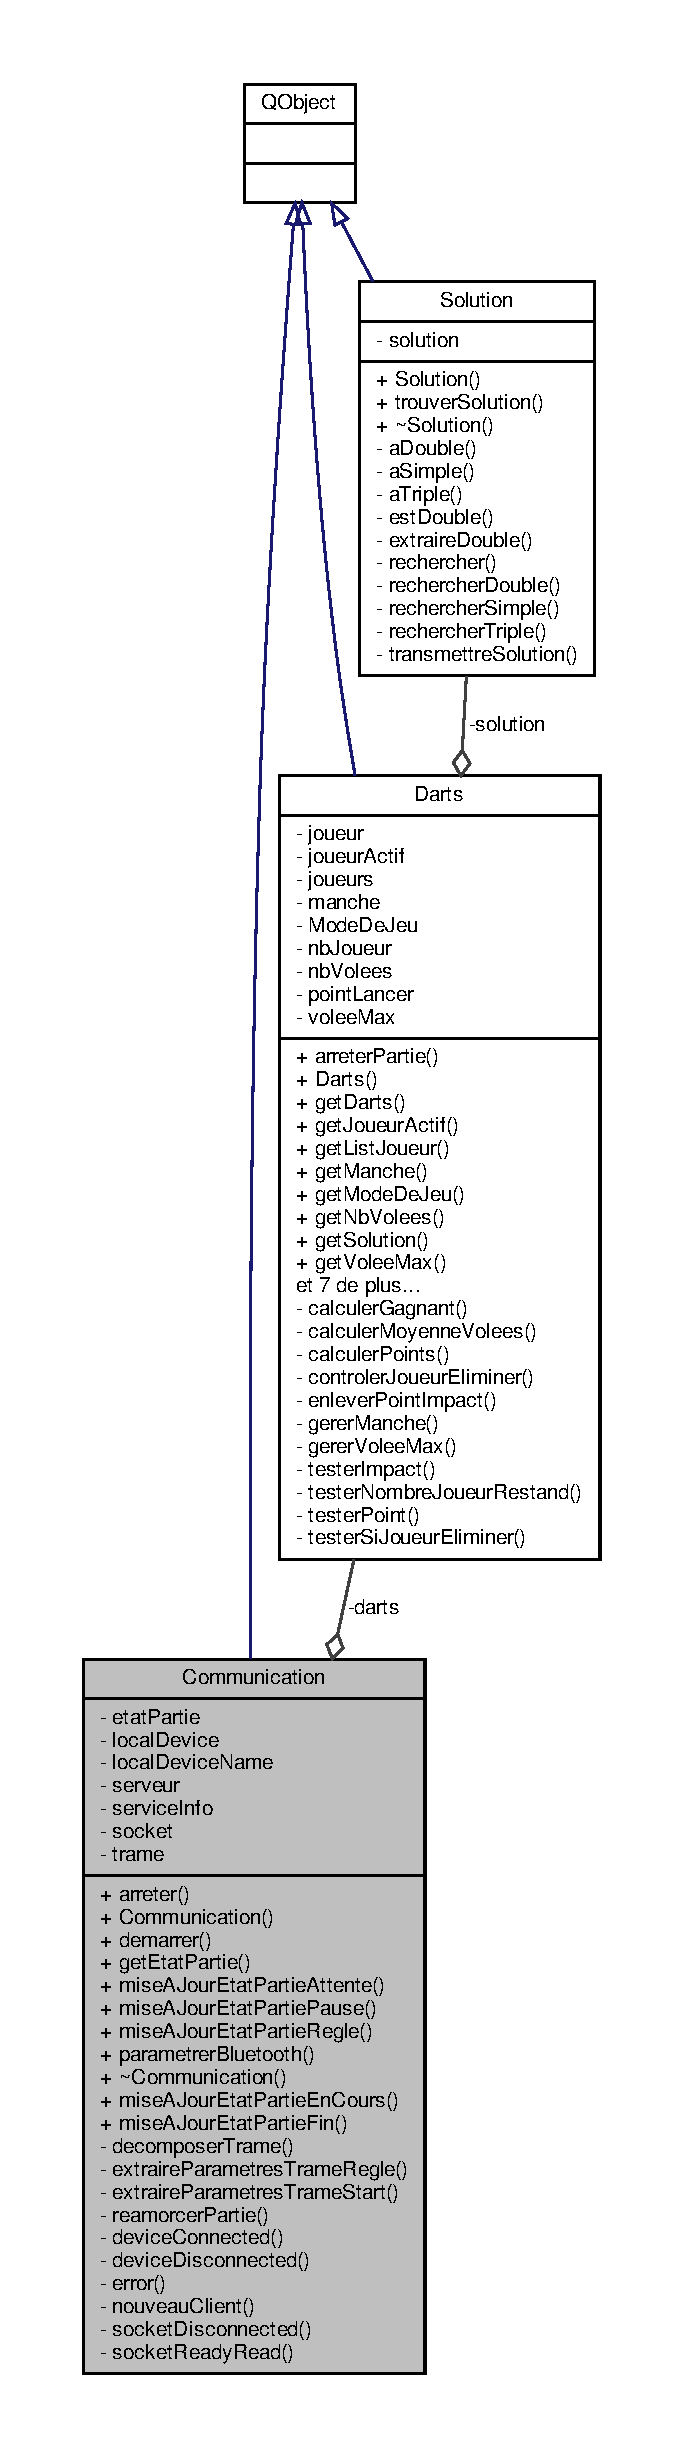
\includegraphics[height=550pt]{class_communication__coll__graph}
\end{center}
\end{figure}
\subsubsection*{Types publics}
\begin{DoxyCompactItemize}
\item 
enum \hyperlink{class_communication_aaa8ce2e87a389c88f4f9a2f07b66ebdd}{Etat\+Partie} \{ \newline
\hyperlink{class_communication_aaa8ce2e87a389c88f4f9a2f07b66ebdda1c2ad067e6861802f9f48fe30001f4dc}{Attente} = 0, 
\hyperlink{class_communication_aaa8ce2e87a389c88f4f9a2f07b66ebdda46965d82c1659dbd82d6b69aad687e54}{En\+Cours} = 1, 
\hyperlink{class_communication_aaa8ce2e87a389c88f4f9a2f07b66ebddafa4e2a4dbf887d1384efe5432e17d57f}{Fin} = 2, 
\hyperlink{class_communication_aaa8ce2e87a389c88f4f9a2f07b66ebddae5ff9fbf58fec2640ed18150aa660bd1}{Pause} = 3, 
\newline
\hyperlink{class_communication_aaa8ce2e87a389c88f4f9a2f07b66ebdda340ac4e51b04541499e50164be9d4d9f}{Regle}
 \}\begin{DoxyCompactList}\small\item\em contient les different etat de la partie \end{DoxyCompactList}
\end{DoxyCompactItemize}
\subsubsection*{Connecteurs publics}
\begin{DoxyCompactItemize}
\item 
void \hyperlink{class_communication_a1f90de1ff5f98de887b9c77664e105c7}{mise\+A\+Jour\+Etat\+Partie\+En\+Cours} ()
\begin{DoxyCompactList}\small\item\em Slot appelé pour mettre à jour l\textquotesingle{}état de la partie à En\+Cours. \end{DoxyCompactList}\item 
void \hyperlink{class_communication_af6b9f4bf3b1df197ce20dccd9b78663f}{mise\+A\+Jour\+Etat\+Partie\+Fin} ()
\begin{DoxyCompactList}\small\item\em Slot appelé pour mettre à jour l\textquotesingle{}état de la partie à Fin. \end{DoxyCompactList}\end{DoxyCompactItemize}
\subsubsection*{Signaux}
\begin{DoxyCompactItemize}
\item 
void \hyperlink{class_communication_aff862483641966b73aa713b419b819a9}{afficher\+Attente\+Connexion} ()
\begin{DoxyCompactList}\small\item\em signal émis quand un appareil se déconnecte \end{DoxyCompactList}\item 
void \hyperlink{class_communication_a4ee52f9b4a1a97967ab2c48a33e0e392}{afficher\+Regle} (Q\+String regle)
\item 
void \hyperlink{class_communication_ae05ddbb1481cfb64f493940b6db8ed29}{appareil\+Connecter} ()
\begin{DoxyCompactList}\small\item\em signal émis quand un nouvel appareil est connecté \end{DoxyCompactList}\item 
void \hyperlink{class_communication_a9cb85e46b57b6dfa9e71408010bfc0a9}{erreur\+Bluetooth} (Q\+String erreur)
\begin{DoxyCompactList}\small\item\em signal emit quand un probleme de configuration bluetooth est detecté \end{DoxyCompactList}\item 
void \hyperlink{class_communication_a369c7aeadc5c5926eb701bdebe53972c}{pause} ()
\begin{DoxyCompactList}\small\item\em signal qui mettra en pause la partie \end{DoxyCompactList}\item 
void \hyperlink{class_communication_a2645730b88adec069200debe05d212c3}{play} ()
\begin{DoxyCompactList}\small\item\em signal qui relancera le chronometrage de la partie la partie \end{DoxyCompactList}\item 
void \hyperlink{class_communication_af79d126304cca4281db4624b1b457ade}{reset\+Partie} ()
\begin{DoxyCompactList}\small\item\em signal qui reinitialisera la partie en cours \end{DoxyCompactList}\end{DoxyCompactItemize}
\subsubsection*{Fonctions membres publiques}
\begin{DoxyCompactItemize}
\item 
void \hyperlink{class_communication_a1f4b02441803f9c8e231cb9f304d776b}{arreter} ()
\begin{DoxyCompactList}\small\item\em Méthode qui arrête le serveur. \end{DoxyCompactList}\item 
\hyperlink{class_communication_a6dd505094f1af1ccd25c6b75c18636d6}{Communication} (\hyperlink{class_darts}{Darts} $\ast$\hyperlink{class_communication_a494d609c206472041468e362d7cfc0e5}{darts}, \hyperlink{class_q_object}{Q\+Object} $\ast$parent=nullptr)
\begin{DoxyCompactList}\small\item\em constructeur de la classe \hyperlink{class_communication}{Communication} \end{DoxyCompactList}\item 
void \hyperlink{class_communication_af29ea9a1c2ce29436f2331c322f6ebbf}{demarrer} ()
\begin{DoxyCompactList}\small\item\em Méthode qui démarre le serveur. \end{DoxyCompactList}\item 
int \hyperlink{class_communication_a977495ad03ddf275aae49184c9a0dd1a}{get\+Etat\+Partie} ()
\begin{DoxyCompactList}\small\item\em Méthode qui retourne l\textquotesingle{}état de la partie. \end{DoxyCompactList}\item 
void \hyperlink{class_communication_a72557be8ab858096e03f08e78e036aeb}{mise\+A\+Jour\+Etat\+Partie\+Attente} ()
\begin{DoxyCompactList}\small\item\em Méthode appelé pour mettre à jour l\textquotesingle{}état de la partie à Attente. \end{DoxyCompactList}\item 
void \hyperlink{class_communication_aaf8fbed545d460414fda14f23d5dca5d}{mise\+A\+Jour\+Etat\+Partie\+Pause} ()
\begin{DoxyCompactList}\small\item\em Méthode appelé pour mettre à jour l\textquotesingle{}état de la partie à Pause. \end{DoxyCompactList}\item 
void \hyperlink{class_communication_a01a86890468a8ecfb900bf15dcab92f2}{mise\+A\+Jour\+Etat\+Partie\+Regle} ()
\begin{DoxyCompactList}\small\item\em Méthode qui met à jour l\textquotesingle{}état de la partie en regle. \end{DoxyCompactList}\item 
void \hyperlink{class_communication_abe2349c8e1d9536a73c8741425ba867f}{parametrer\+Bluetooth} ()
\begin{DoxyCompactList}\small\item\em Méthode qui configure la connexion Bluetooth en mode serveur. \end{DoxyCompactList}\item 
\hyperlink{class_communication_a75ba08ce908d45251e28e4c1db94e6f4}{$\sim$\+Communication} ()
\begin{DoxyCompactList}\small\item\em destructeur de la classe \hyperlink{class_communication}{Communication} \end{DoxyCompactList}\end{DoxyCompactItemize}
\subsubsection*{Connecteurs privés}
\begin{DoxyCompactItemize}
\item 
void \hyperlink{class_communication_a33db5c9db5da71c20c8c544d1de4eb9a}{device\+Connected} (const Q\+Bluetooth\+Address \&adresse)
\begin{DoxyCompactList}\small\item\em Slot appelé quand un nouvel appareil est connecté \end{DoxyCompactList}\item 
void \hyperlink{class_communication_a0ee021f517bb0e3f7149ed13f8faf0b1}{device\+Disconnected} (const Q\+Bluetooth\+Address \&adresse)
\begin{DoxyCompactList}\small\item\em Slot appelé quand un appareil est déconnecté \end{DoxyCompactList}\item 
void \hyperlink{class_communication_af95addb3c2bc178cfd7c92c6f94680a4}{error} (Q\+Bluetooth\+Local\+Device\+::\+Error erreur)
\begin{DoxyCompactList}\small\item\em Slot appelé quand il y a une erreur avec l\textquotesingle{}appareil bluetooth. \end{DoxyCompactList}\item 
void \hyperlink{class_communication_ac1bc22603b6e05389f94890b745aac4f}{nouveau\+Client} ()
\begin{DoxyCompactList}\small\item\em Slot appelé quand un nouveau client veut se connecter. \end{DoxyCompactList}\item 
void \hyperlink{class_communication_a44f863f2c70f4be652224240447c9fe0}{socket\+Disconnected} ()
\begin{DoxyCompactList}\small\item\em Slot appelé quand la communication est deconnectée. \end{DoxyCompactList}\item 
void \hyperlink{class_communication_a0576a95d1f3c4ec49172a1040cfbeedf}{socket\+Ready\+Read} ()
\begin{DoxyCompactList}\small\item\em Slot appelé quand une nouvelle trame est disponible. \end{DoxyCompactList}\end{DoxyCompactItemize}
\subsubsection*{Fonctions membres privées}
\begin{DoxyCompactItemize}
\item 
void \hyperlink{class_communication_aaf5333662717e69837d2d39164e5a303}{decomposer\+Trame} ()
\begin{DoxyCompactList}\small\item\em Méthode qui decompose la trame reçue. \end{DoxyCompactList}\item 
void \hyperlink{class_communication_aa7fd74ea88ca7b28cb00e6b74b902394}{extraire\+Parametres\+Trame\+Regle} ()
\begin{DoxyCompactList}\small\item\em Méthode qui decompose la trame regle. \end{DoxyCompactList}\item 
void \hyperlink{class_communication_a31f998e3410e7a1d9e65a05a5d51a9b9}{extraire\+Parametres\+Trame\+Start} (Q\+String\+List \&joueurs, Q\+String \&mode\+Jeu)
\begin{DoxyCompactList}\small\item\em Méthode qui extrait les paramètres de la trame S\+T\+A\+RT. \end{DoxyCompactList}\item 
void \hyperlink{class_communication_a56ed5d11756b1f9efcca609b9f8a59c9}{reamorcer\+Partie} ()
\begin{DoxyCompactList}\small\item\em Méthode qui reinitialise la partie. \end{DoxyCompactList}\end{DoxyCompactItemize}
\subsubsection*{Attributs privés}
\begin{DoxyCompactItemize}
\item 
\hyperlink{class_darts}{Darts} $\ast$ \hyperlink{class_communication_a494d609c206472041468e362d7cfc0e5}{darts}
\begin{DoxyCompactList}\small\item\em Association avec l\textquotesingle{}objet darts. \end{DoxyCompactList}\item 
\hyperlink{class_communication_aaa8ce2e87a389c88f4f9a2f07b66ebdd}{Etat\+Partie} \hyperlink{class_communication_a2539ded2780db2c732690c585c768c96}{etat\+Partie}
\begin{DoxyCompactList}\small\item\em L\textquotesingle{}état de la partie. \end{DoxyCompactList}\item 
Q\+Bluetooth\+Local\+Device \hyperlink{class_communication_a6281796eab7523bef6be1a766e0e906f}{local\+Device}
\begin{DoxyCompactList}\small\item\em L\textquotesingle{}interface Bluetooth de la Raspberry Pi. \end{DoxyCompactList}\item 
Q\+String \hyperlink{class_communication_aa70c6b4acb921b03ffa8b8b044e87a94}{local\+Device\+Name}
\begin{DoxyCompactList}\small\item\em Nom du peripherique local. \end{DoxyCompactList}\item 
Q\+Bluetooth\+Server $\ast$ \hyperlink{class_communication_a6384747297d6efa9e8fd2fc79ed0c269}{serveur}
\begin{DoxyCompactList}\small\item\em Le serveur Bluetooth. \end{DoxyCompactList}\item 
Q\+Bluetooth\+Service\+Info \hyperlink{class_communication_aa7f9ee5e5d90336a56857ebc229e4274}{service\+Info}
\begin{DoxyCompactList}\small\item\em Informations sur le service bluetooth. \end{DoxyCompactList}\item 
Q\+Bluetooth\+Socket $\ast$ \hyperlink{class_communication_aa4ddc3151b305db0135d5826384645cc}{socket}
\begin{DoxyCompactList}\small\item\em La socket de communication Bluetooth. \end{DoxyCompactList}\item 
Q\+String \hyperlink{class_communication_ac8f5004bfaaf7f538ba5ae93255f772b}{trame}
\begin{DoxyCompactList}\small\item\em La trame recue. \end{DoxyCompactList}\end{DoxyCompactItemize}


\subsubsection{Description détaillée}
Déclaration de la classe \hyperlink{class_communication}{Communication} via la liaison Bluetooth (Module Ecran-\/\+D\+A\+R\+TS) 

Cette classe s\textquotesingle{}occupe de la partie communication Bluetooth en mode serveur (configuration, réception et traitement des trames du protocole D\+A\+RT) 

Définition à la ligne \hyperlink{communication_8h_source_l00041}{41} du fichier \hyperlink{communication_8h_source}{communication.\+h}.



\subsubsection{Documentation des énumérations membres}
\mbox{\Hypertarget{class_communication_aaa8ce2e87a389c88f4f9a2f07b66ebdd}\label{class_communication_aaa8ce2e87a389c88f4f9a2f07b66ebdd}} 
\index{Communication@{Communication}!Etat\+Partie@{Etat\+Partie}}
\index{Etat\+Partie@{Etat\+Partie}!Communication@{Communication}}
\paragraph{\texorpdfstring{Etat\+Partie}{EtatPartie}}
{\footnotesize\ttfamily enum \hyperlink{class_communication_aaa8ce2e87a389c88f4f9a2f07b66ebdd}{Communication\+::\+Etat\+Partie}}



contient les different etat de la partie 

\begin{DoxyEnumFields}{Valeurs énumérées}
\raisebox{\heightof{T}}[0pt][0pt]{\index{Attente@{Attente}!Communication@{Communication}}\index{Communication@{Communication}!Attente@{Attente}}}\mbox{\Hypertarget{class_communication_aaa8ce2e87a389c88f4f9a2f07b66ebdda1c2ad067e6861802f9f48fe30001f4dc}\label{class_communication_aaa8ce2e87a389c88f4f9a2f07b66ebdda1c2ad067e6861802f9f48fe30001f4dc}} 
Attente&\\
\hline

\raisebox{\heightof{T}}[0pt][0pt]{\index{En\+Cours@{En\+Cours}!Communication@{Communication}}\index{Communication@{Communication}!En\+Cours@{En\+Cours}}}\mbox{\Hypertarget{class_communication_aaa8ce2e87a389c88f4f9a2f07b66ebdda46965d82c1659dbd82d6b69aad687e54}\label{class_communication_aaa8ce2e87a389c88f4f9a2f07b66ebdda46965d82c1659dbd82d6b69aad687e54}} 
En\+Cours&\\
\hline

\raisebox{\heightof{T}}[0pt][0pt]{\index{Fin@{Fin}!Communication@{Communication}}\index{Communication@{Communication}!Fin@{Fin}}}\mbox{\Hypertarget{class_communication_aaa8ce2e87a389c88f4f9a2f07b66ebddafa4e2a4dbf887d1384efe5432e17d57f}\label{class_communication_aaa8ce2e87a389c88f4f9a2f07b66ebddafa4e2a4dbf887d1384efe5432e17d57f}} 
Fin&\\
\hline

\raisebox{\heightof{T}}[0pt][0pt]{\index{Pause@{Pause}!Communication@{Communication}}\index{Communication@{Communication}!Pause@{Pause}}}\mbox{\Hypertarget{class_communication_aaa8ce2e87a389c88f4f9a2f07b66ebddae5ff9fbf58fec2640ed18150aa660bd1}\label{class_communication_aaa8ce2e87a389c88f4f9a2f07b66ebddae5ff9fbf58fec2640ed18150aa660bd1}} 
Pause&\\
\hline

\raisebox{\heightof{T}}[0pt][0pt]{\index{Regle@{Regle}!Communication@{Communication}}\index{Communication@{Communication}!Regle@{Regle}}}\mbox{\Hypertarget{class_communication_aaa8ce2e87a389c88f4f9a2f07b66ebdda340ac4e51b04541499e50164be9d4d9f}\label{class_communication_aaa8ce2e87a389c88f4f9a2f07b66ebdda340ac4e51b04541499e50164be9d4d9f}} 
Regle&\\
\hline

\end{DoxyEnumFields}


Définition à la ligne \hyperlink{communication_8h_source_l00061}{61} du fichier \hyperlink{communication_8h_source}{communication.\+h}.


\begin{DoxyCode}
00062     \{
00063         \hyperlink{class_communication_aaa8ce2e87a389c88f4f9a2f07b66ebdda1c2ad067e6861802f9f48fe30001f4dc}{Attente} = 0,
00064         \hyperlink{class_communication_aaa8ce2e87a389c88f4f9a2f07b66ebdda46965d82c1659dbd82d6b69aad687e54}{EnCours} = 1,
00065         \hyperlink{class_communication_aaa8ce2e87a389c88f4f9a2f07b66ebddafa4e2a4dbf887d1384efe5432e17d57f}{Fin} = 2,
00066         \hyperlink{class_communication_aaa8ce2e87a389c88f4f9a2f07b66ebddae5ff9fbf58fec2640ed18150aa660bd1}{Pause} = 3,
00067         \hyperlink{class_communication_aaa8ce2e87a389c88f4f9a2f07b66ebdda340ac4e51b04541499e50164be9d4d9f}{Regle}       \textcolor{comment}{//État attente pendant la lecture des règles, seule une trame reset peut être reçu
       pour arrêter la lecture.}
00068     \};
\end{DoxyCode}


\subsubsection{Documentation des constructeurs et destructeur}
\mbox{\Hypertarget{class_communication_a6dd505094f1af1ccd25c6b75c18636d6}\label{class_communication_a6dd505094f1af1ccd25c6b75c18636d6}} 
\index{Communication@{Communication}!Communication@{Communication}}
\index{Communication@{Communication}!Communication@{Communication}}
\paragraph{\texorpdfstring{Communication()}{Communication()}}
{\footnotesize\ttfamily Communication\+::\+Communication (\begin{DoxyParamCaption}\item[{\hyperlink{class_darts}{Darts} $\ast$}]{darts,  }\item[{\hyperlink{class_q_object}{Q\+Object} $\ast$}]{parent = {\ttfamily nullptr} }\end{DoxyParamCaption})\hspace{0.3cm}{\ttfamily [explicit]}}



constructeur de la classe \hyperlink{class_communication}{Communication} 


\begin{DoxyParams}{Paramètres}
{\em darts} & \\
\hline
{\em parent} & \\
\hline
\end{DoxyParams}


Définition à la ligne \hyperlink{communication_8cpp_source_l00022}{22} du fichier \hyperlink{communication_8cpp_source}{communication.\+cpp}.



Références \hyperlink{communication_8cpp_source_l00382}{mise\+A\+Jour\+Etat\+Partie\+Attente()}, et \hyperlink{communication_8cpp_source_l00059}{parametrer\+Bluetooth()}.


\begin{DoxyCode}
00022                                                           : \hyperlink{class_q_object}{QObject}(parent), 
      \hyperlink{class_communication_a494d609c206472041468e362d7cfc0e5}{darts}(darts), \hyperlink{class_communication_a6384747297d6efa9e8fd2fc79ed0c269}{serveur}(\textcolor{keyword}{nullptr}), \hyperlink{class_communication_aa4ddc3151b305db0135d5826384645cc}{socket}(\textcolor{keyword}{nullptr}), 
      \hyperlink{class_communication_aa70c6b4acb921b03ffa8b8b044e87a94}{localDeviceName}(\textcolor{stringliteral}{"Ecran-Darts"}), \hyperlink{class_communication_ac8f5004bfaaf7f538ba5ae93255f772b}{trame}(\textcolor{stringliteral}{""})
00023 \{
00024     qDebug() << Q\_FUNC\_INFO;
00025 
00026     \hyperlink{class_communication_abe2349c8e1d9536a73c8741425ba867f}{parametrerBluetooth}();
00027 
00028     \hyperlink{class_communication_a72557be8ab858096e03f08e78e036aeb}{miseAJourEtatPartieAttente}();
00029 \}
\end{DoxyCode}
\mbox{\Hypertarget{class_communication_a75ba08ce908d45251e28e4c1db94e6f4}\label{class_communication_a75ba08ce908d45251e28e4c1db94e6f4}} 
\index{Communication@{Communication}!````~Communication@{$\sim$\+Communication}}
\index{````~Communication@{$\sim$\+Communication}!Communication@{Communication}}
\paragraph{\texorpdfstring{$\sim$\+Communication()}{~Communication()}}
{\footnotesize\ttfamily Communication\+::$\sim$\+Communication (\begin{DoxyParamCaption}{ }\end{DoxyParamCaption})}



destructeur de la classe \hyperlink{class_communication}{Communication} 



Définition à la ligne \hyperlink{communication_8cpp_source_l00036}{36} du fichier \hyperlink{communication_8cpp_source}{communication.\+cpp}.



Références \hyperlink{communication_8cpp_source_l00121}{arreter()}, et \hyperlink{communication_8h_source_l00096}{local\+Device}.


\begin{DoxyCode}
00037 \{
00038     \hyperlink{class_communication_a1f4b02441803f9c8e231cb9f304d776b}{arreter}();
00039     \hyperlink{class_communication_a6281796eab7523bef6be1a766e0e906f}{localDevice}.setHostMode(QBluetoothLocalDevice::HostPoweredOff);
00040     qDebug() << Q\_FUNC\_INFO;
00041 \}
\end{DoxyCode}


\subsubsection{Documentation des fonctions membres}
\mbox{\Hypertarget{class_communication_aff862483641966b73aa713b419b819a9}\label{class_communication_aff862483641966b73aa713b419b819a9}} 
\index{Communication@{Communication}!afficher\+Attente\+Connexion@{afficher\+Attente\+Connexion}}
\index{afficher\+Attente\+Connexion@{afficher\+Attente\+Connexion}!Communication@{Communication}}
\paragraph{\texorpdfstring{afficher\+Attente\+Connexion}{afficherAttenteConnexion}}
{\footnotesize\ttfamily void Communication\+::afficher\+Attente\+Connexion (\begin{DoxyParamCaption}{ }\end{DoxyParamCaption})\hspace{0.3cm}{\ttfamily [signal]}}



signal émis quand un appareil se déconnecte 



Référencé par \hyperlink{communication_8cpp_source_l00353}{device\+Disconnected()}.

\mbox{\Hypertarget{class_communication_a4ee52f9b4a1a97967ab2c48a33e0e392}\label{class_communication_a4ee52f9b4a1a97967ab2c48a33e0e392}} 
\index{Communication@{Communication}!afficher\+Regle@{afficher\+Regle}}
\index{afficher\+Regle@{afficher\+Regle}!Communication@{Communication}}
\paragraph{\texorpdfstring{afficher\+Regle}{afficherRegle}}
{\footnotesize\ttfamily void Communication\+::afficher\+Regle (\begin{DoxyParamCaption}\item[{Q\+String}]{regle }\end{DoxyParamCaption})\hspace{0.3cm}{\ttfamily [signal]}}



Référencé par \hyperlink{communication_8cpp_source_l00279}{extraire\+Parametres\+Trame\+Regle()}, et \hyperlink{communication_8cpp_source_l00243}{extraire\+Parametres\+Trame\+Start()}.

\mbox{\Hypertarget{class_communication_ae05ddbb1481cfb64f493940b6db8ed29}\label{class_communication_ae05ddbb1481cfb64f493940b6db8ed29}} 
\index{Communication@{Communication}!appareil\+Connecter@{appareil\+Connecter}}
\index{appareil\+Connecter@{appareil\+Connecter}!Communication@{Communication}}
\paragraph{\texorpdfstring{appareil\+Connecter}{appareilConnecter}}
{\footnotesize\ttfamily void Communication\+::appareil\+Connecter (\begin{DoxyParamCaption}{ }\end{DoxyParamCaption})\hspace{0.3cm}{\ttfamily [signal]}}



signal émis quand un nouvel appareil est connecté 



Référencé par \hyperlink{communication_8cpp_source_l00329}{device\+Connected()}.

\mbox{\Hypertarget{class_communication_a1f4b02441803f9c8e231cb9f304d776b}\label{class_communication_a1f4b02441803f9c8e231cb9f304d776b}} 
\index{Communication@{Communication}!arreter@{arreter}}
\index{arreter@{arreter}!Communication@{Communication}}
\paragraph{\texorpdfstring{arreter()}{arreter()}}
{\footnotesize\ttfamily void Communication\+::arreter (\begin{DoxyParamCaption}{ }\end{DoxyParamCaption})}



Méthode qui arrête le serveur. 

arrete le serveur 

Définition à la ligne \hyperlink{communication_8cpp_source_l00121}{121} du fichier \hyperlink{communication_8cpp_source}{communication.\+cpp}.



Références \hyperlink{communication_8h_source_l00096}{local\+Device}, \hyperlink{communication_8h_source_l00094}{serveur}, \hyperlink{communication_8h_source_l00097}{service\+Info}, et \hyperlink{communication_8h_source_l00095}{socket}.



Référencé par \hyperlink{communication_8cpp_source_l00036}{$\sim$\+Communication()}.


\begin{DoxyCode}
00122 \{
00123     \textcolor{keywordflow}{if} (!\hyperlink{class_communication_a6281796eab7523bef6be1a766e0e906f}{localDevice}.isValid())
00124         \textcolor{keywordflow}{return};
00125 
00126     \textcolor{keywordflow}{if} (!\hyperlink{class_communication_a6384747297d6efa9e8fd2fc79ed0c269}{serveur})
00127         \textcolor{keywordflow}{return};
00128 
00129     \hyperlink{class_communication_aa7f9ee5e5d90336a56857ebc229e4274}{serviceInfo}.unregisterService();
00130 
00131     \textcolor{keywordflow}{if} (\hyperlink{class_communication_aa4ddc3151b305db0135d5826384645cc}{socket})
00132     \{
00133         \textcolor{keywordflow}{if} (\hyperlink{class_communication_aa4ddc3151b305db0135d5826384645cc}{socket}->isOpen())
00134         \{
00135            \hyperlink{class_communication_aa4ddc3151b305db0135d5826384645cc}{socket}->close();
00136         \}
00137         \textcolor{keyword}{delete} \hyperlink{class_communication_aa4ddc3151b305db0135d5826384645cc}{socket};
00138         \hyperlink{class_communication_aa4ddc3151b305db0135d5826384645cc}{socket} = \textcolor{keyword}{nullptr};
00139     \}
00140 
00141     \textcolor{keyword}{delete} \hyperlink{class_communication_a6384747297d6efa9e8fd2fc79ed0c269}{serveur};
00142     \hyperlink{class_communication_a6384747297d6efa9e8fd2fc79ed0c269}{serveur} = \textcolor{keyword}{nullptr};
00143 \}
\end{DoxyCode}
\mbox{\Hypertarget{class_communication_aaf5333662717e69837d2d39164e5a303}\label{class_communication_aaf5333662717e69837d2d39164e5a303}} 
\index{Communication@{Communication}!decomposer\+Trame@{decomposer\+Trame}}
\index{decomposer\+Trame@{decomposer\+Trame}!Communication@{Communication}}
\paragraph{\texorpdfstring{decomposer\+Trame()}{decomposerTrame()}}
{\footnotesize\ttfamily void Communication\+::decomposer\+Trame (\begin{DoxyParamCaption}{ }\end{DoxyParamCaption})\hspace{0.3cm}{\ttfamily [private]}}



Méthode qui decompose la trame reçue. 

Méthode qui decompose la trame reçue et signale l\textquotesingle{}état en fonction du type de trame. \$\+D\+A\+RT;S\+T\+A\+RT;501;1;2;fabien;erwan

\$\+D\+A\+RT;G\+A\+ME;3;7

\$\+D\+A\+RT;R\+E\+G\+LE

\$\+D\+A\+RT;P\+A\+U\+SE

\$\+D\+A\+RT;P\+L\+AY

\$\+D\+A\+RT;S\+T\+OP 

Définition à la ligne \hyperlink{communication_8cpp_source_l00188}{188} du fichier \hyperlink{communication_8cpp_source}{communication.\+cpp}.



Références \hyperlink{darts_8cpp_source_l00422}{Darts\+::arreter\+Partie()}, \hyperlink{communication_8h_source_l00093}{darts}, \hyperlink{communication_8h_source_l00030}{D\+E\+L\+I\+M\+I\+T\+E\+U\+R\+\_\+\+F\+IN}, \hyperlink{communication_8h_source_l00100}{etat\+Partie}, \hyperlink{communication_8cpp_source_l00279}{extraire\+Parametres\+Trame\+Regle()}, \hyperlink{communication_8cpp_source_l00243}{extraire\+Parametres\+Trame\+Start()}, \hyperlink{communication_8cpp_source_l00415}{mise\+A\+Jour\+Etat\+Partie\+En\+Cours()}, \hyperlink{communication_8cpp_source_l00393}{mise\+A\+Jour\+Etat\+Partie\+Pause()}, \hyperlink{class_communication_a369c7aeadc5c5926eb701bdebe53972c}{pause()}, \hyperlink{class_communication_a2645730b88adec069200debe05d212c3}{play()}, \hyperlink{communication_8cpp_source_l00305}{reamorcer\+Partie()}, \hyperlink{darts_8cpp_source_l00223}{Darts\+::receptionner\+Impact()}, \hyperlink{darts_8cpp_source_l00184}{Darts\+::reinitialiser\+Partie()}, \hyperlink{class_communication_af79d126304cca4281db4624b1b457ade}{reset\+Partie()}, \hyperlink{communication_8h_source_l00099}{trame}, et \hyperlink{communication_8h_source_l00024}{T\+Y\+P\+E\+\_\+\+T\+R\+A\+ME}.



Référencé par \hyperlink{communication_8cpp_source_l00166}{socket\+Ready\+Read()}.


\begin{DoxyCode}
00189 \{
00190     \textcolor{keywordflow}{if}(\hyperlink{class_communication_ac8f5004bfaaf7f538ba5ae93255f772b}{trame}.startsWith(\hyperlink{communication_8h_a8da23fa25560c54c52884746a5d1cc69}{TYPE\_TRAME}) && \hyperlink{class_communication_ac8f5004bfaaf7f538ba5ae93255f772b}{trame}.endsWith(
      \hyperlink{communication_8h_aafcc0c7b4996f7783c9f4e766a233487}{DELIMITEUR\_FIN})) \textcolor{comment}{//test si la trame est valide}
00191     \{
00192         \hyperlink{class_communication_ac8f5004bfaaf7f538ba5ae93255f772b}{trame}.remove(\hyperlink{communication_8h_aafcc0c7b4996f7783c9f4e766a233487}{DELIMITEUR\_FIN});
00193         \textcolor{keywordflow}{if}(\hyperlink{class_communication_ac8f5004bfaaf7f538ba5ae93255f772b}{trame}.contains(\textcolor{stringliteral}{"START"}) && (\hyperlink{class_communication_a2539ded2780db2c732690c585c768c96}{etatPartie} == EtatPartie::Attente || 
      \hyperlink{class_communication_a2539ded2780db2c732690c585c768c96}{etatPartie} == EtatPartie::Fin))      
00194         \{
00195             emit \hyperlink{class_communication_af79d126304cca4281db4624b1b457ade}{resetPartie}();
00196             \hyperlink{class_communication_a494d609c206472041468e362d7cfc0e5}{darts}->\hyperlink{class_darts_a70c68ed8bd56b63df203c25e6ed14f3b}{reinitialiserPartie}();
00197 
00198             QString modeJeu;
00199             QStringList joueurs;
00200 
00201             \hyperlink{class_communication_a31f998e3410e7a1d9e65a05a5d51a9b9}{extraireParametresTrameStart}(joueurs, modeJeu);
00202         \}
00203         \textcolor{keywordflow}{else} \textcolor{keywordflow}{if}(\hyperlink{class_communication_ac8f5004bfaaf7f538ba5ae93255f772b}{trame}.contains(\textcolor{stringliteral}{"GAME"}) && \hyperlink{class_communication_a2539ded2780db2c732690c585c768c96}{etatPartie} == EtatPartie::EnCours)      
00204         \{
00205             \hyperlink{class_communication_a494d609c206472041468e362d7cfc0e5}{darts}->\hyperlink{class_darts_a196bc4307c631310f641606012ab9e05}{receptionnerImpact}(\hyperlink{class_communication_ac8f5004bfaaf7f538ba5ae93255f772b}{trame}.section(\textcolor{stringliteral}{";"},2,2).toInt(), 
      \hyperlink{class_communication_ac8f5004bfaaf7f538ba5ae93255f772b}{trame}.section(\textcolor{stringliteral}{";"},3,3).toInt());
00206         \}
00207         \textcolor{keywordflow}{else} \textcolor{keywordflow}{if}(\hyperlink{class_communication_ac8f5004bfaaf7f538ba5ae93255f772b}{trame}.contains(\textcolor{stringliteral}{"REGLE"})&& \hyperlink{class_communication_a2539ded2780db2c732690c585c768c96}{etatPartie} != EtatPartie::Regle)   
00208         \{
00209             \hyperlink{class_communication_aa7fd74ea88ca7b28cb00e6b74b902394}{extraireParametresTrameRegle}();
00210         \}
00211         \textcolor{keywordflow}{else} \textcolor{keywordflow}{if}(\hyperlink{class_communication_ac8f5004bfaaf7f538ba5ae93255f772b}{trame}.contains(\textcolor{stringliteral}{"PAUSE"}) && \hyperlink{class_communication_a2539ded2780db2c732690c585c768c96}{etatPartie} == EtatPartie::EnCours)     
00212         \{
00213             emit \hyperlink{class_communication_a369c7aeadc5c5926eb701bdebe53972c}{pause}();
00214             \hyperlink{class_communication_aaf8fbed545d460414fda14f23d5dca5d}{miseAJourEtatPartiePause}();
00215         \}
00216         \textcolor{keywordflow}{else} \textcolor{keywordflow}{if}(\hyperlink{class_communication_ac8f5004bfaaf7f538ba5ae93255f772b}{trame}.contains(\textcolor{stringliteral}{"PLAY"}) && \hyperlink{class_communication_a2539ded2780db2c732690c585c768c96}{etatPartie} == EtatPartie::Pause)       
00217         \{
00218             emit \hyperlink{class_communication_a2645730b88adec069200debe05d212c3}{play}();
00219             \hyperlink{class_communication_a1f90de1ff5f98de887b9c77664e105c7}{miseAJourEtatPartieEnCours}();
00220         \}
00221         \textcolor{keywordflow}{else} \textcolor{keywordflow}{if}(\hyperlink{class_communication_ac8f5004bfaaf7f538ba5ae93255f772b}{trame}.contains(\textcolor{stringliteral}{"RESET"})) \textcolor{comment}{// quelque soit l'état de la partie    /** $DART;RESET */}
00222         \{
00223             \hyperlink{class_communication_a56ed5d11756b1f9efcca609b9f8a59c9}{reamorcerPartie}();
00224         \}
00225         \textcolor{keywordflow}{else} \textcolor{keywordflow}{if}(\hyperlink{class_communication_ac8f5004bfaaf7f538ba5ae93255f772b}{trame}.contains(\textcolor{stringliteral}{"STOP"}) && (\hyperlink{class_communication_a2539ded2780db2c732690c585c768c96}{etatPartie} == EtatPartie::EnCours || 
      \hyperlink{class_communication_a2539ded2780db2c732690c585c768c96}{etatPartie} == EtatPartie::Pause))  
00226         \{
00227             \hyperlink{class_communication_a494d609c206472041468e362d7cfc0e5}{darts}->\hyperlink{class_darts_aa9685f754172d995cdd04d39d9651227}{arreterPartie}();
00228         \}
00229         \textcolor{keywordflow}{else}
00230         \{
00231             qDebug() << Q\_FUNC\_INFO << \textcolor{stringliteral}{"Trame erreur: "} << \hyperlink{class_communication_ac8f5004bfaaf7f538ba5ae93255f772b}{trame};
00232         \}
00233     \}
00234 \}
\end{DoxyCode}
\mbox{\Hypertarget{class_communication_af29ea9a1c2ce29436f2331c322f6ebbf}\label{class_communication_af29ea9a1c2ce29436f2331c322f6ebbf}} 
\index{Communication@{Communication}!demarrer@{demarrer}}
\index{demarrer@{demarrer}!Communication@{Communication}}
\paragraph{\texorpdfstring{demarrer()}{demarrer()}}
{\footnotesize\ttfamily void Communication\+::demarrer (\begin{DoxyParamCaption}{ }\end{DoxyParamCaption})}



Méthode qui démarre le serveur. 

Démarre le serveur. 

Définition à la ligne \hyperlink{communication_8cpp_source_l00101}{101} du fichier \hyperlink{communication_8cpp_source}{communication.\+cpp}.



Références \hyperlink{communication_8h_source_l00096}{local\+Device}, \hyperlink{communication_8cpp_source_l00150}{nouveau\+Client()}, \hyperlink{communication_8h_source_l00094}{serveur}, \hyperlink{communication_8h_source_l00097}{service\+Info}, \hyperlink{communication_8h_a28fc73dd6a464ea3a1cdb210ee7a1925}{service\+Nom()}, et \hyperlink{communication_8h_a50c84e57d8bf82d8048cc731a5679b64}{service\+Uuid()}.



Référencé par \hyperlink{ihm_8cpp_source_l00026}{Ihm\+::\+Ihm()}.


\begin{DoxyCode}
00102 \{
00103     \textcolor{keywordflow}{if} (!\hyperlink{class_communication_a6281796eab7523bef6be1a766e0e906f}{localDevice}.isValid())
00104         \textcolor{keywordflow}{return};
00105 
00106     \textcolor{keywordflow}{if} (!\hyperlink{class_communication_a6384747297d6efa9e8fd2fc79ed0c269}{serveur})   \textcolor{comment}{//Démarre le serveur s'il n'est pas déjà démarré}
00107     \{
00108         \hyperlink{class_communication_a6384747297d6efa9e8fd2fc79ed0c269}{serveur} = \textcolor{keyword}{new} QBluetoothServer(QBluetoothServiceInfo::RfcommProtocol, \textcolor{keyword}{this});
00109         connect(\hyperlink{class_communication_a6384747297d6efa9e8fd2fc79ed0c269}{serveur}, SIGNAL(newConnection()), \textcolor{keyword}{this}, SLOT(
      \hyperlink{class_communication_ac1bc22603b6e05389f94890b745aac4f}{nouveauClient}()));
00110 
00111         QBluetoothUuid uuid = QBluetoothUuid(\hyperlink{communication_8h_a50c84e57d8bf82d8048cc731a5679b64}{serviceUuid});
00112         \hyperlink{class_communication_aa7f9ee5e5d90336a56857ebc229e4274}{serviceInfo} = \hyperlink{class_communication_a6384747297d6efa9e8fd2fc79ed0c269}{serveur}->listen(uuid, \hyperlink{communication_8h_a28fc73dd6a464ea3a1cdb210ee7a1925}{serviceNom});
00113     \}
00114 \}
\end{DoxyCode}
\mbox{\Hypertarget{class_communication_a33db5c9db5da71c20c8c544d1de4eb9a}\label{class_communication_a33db5c9db5da71c20c8c544d1de4eb9a}} 
\index{Communication@{Communication}!device\+Connected@{device\+Connected}}
\index{device\+Connected@{device\+Connected}!Communication@{Communication}}
\paragraph{\texorpdfstring{device\+Connected}{deviceConnected}}
{\footnotesize\ttfamily void Communication\+::device\+Connected (\begin{DoxyParamCaption}\item[{const Q\+Bluetooth\+Address \&}]{adresse }\end{DoxyParamCaption})\hspace{0.3cm}{\ttfamily [private]}, {\ttfamily [slot]}}



Slot appelé quand un nouvel appareil est connecté 

Méthode appelée quand l\textquotesingle{}appareil est connecté


\begin{DoxyParams}{Paramètres}
{\em adresse} & \\
\hline
\end{DoxyParams}


Définition à la ligne \hyperlink{communication_8cpp_source_l00329}{329} du fichier \hyperlink{communication_8cpp_source}{communication.\+cpp}.



Références \hyperlink{class_communication_ae05ddbb1481cfb64f493940b6db8ed29}{appareil\+Connecter()}, \hyperlink{communication_8h_source_l00100}{etat\+Partie}, \hyperlink{communication_8h_source_l00096}{local\+Device}, \hyperlink{communication_8cpp_source_l00415}{mise\+A\+Jour\+Etat\+Partie\+En\+Cours()}, et \hyperlink{class_communication_a2645730b88adec069200debe05d212c3}{play()}.



Référencé par \hyperlink{communication_8cpp_source_l00059}{parametrer\+Bluetooth()}.


\begin{DoxyCode}
00330 \{
00331     qDebug() << Q\_FUNC\_INFO << adresse << \hyperlink{class_communication_a6281796eab7523bef6be1a766e0e906f}{localDevice}.pairingStatus(adresse);
00332     QString message = QString::fromUtf8(\textcolor{stringliteral}{"Demande connexion du client "}) + adresse.toString();
00333     emit \hyperlink{class_communication_ae05ddbb1481cfb64f493940b6db8ed29}{appareilConnecter}();
00334     \textcolor{keywordflow}{if} (\hyperlink{class_communication_a6281796eab7523bef6be1a766e0e906f}{localDevice}.pairingStatus(adresse) == QBluetoothLocalDevice::Paired || 
      \hyperlink{class_communication_a6281796eab7523bef6be1a766e0e906f}{localDevice}.pairingStatus(adresse) == QBluetoothLocalDevice::AuthorizedPaired)
00335         message += \textcolor{stringliteral}{" ["} + QString::fromUtf8(\textcolor{stringliteral}{"appairé"}) + \textcolor{stringliteral}{"]"};
00336     \textcolor{keywordflow}{else}
00337         message += \textcolor{stringliteral}{" ["} + QString::fromUtf8(\textcolor{stringliteral}{"non appairé"}) + \textcolor{stringliteral}{"]"} ;
00338     qDebug() << message << endl;
00339 
00340     \textcolor{keywordflow}{if}(\hyperlink{class_communication_a2539ded2780db2c732690c585c768c96}{etatPartie} == EtatPartie::Pause) \textcolor{comment}{// si l'appareil est reconnecte, la partie reprend}
00341     \{
00342         emit \hyperlink{class_communication_a2645730b88adec069200debe05d212c3}{play}();
00343         \hyperlink{class_communication_a1f90de1ff5f98de887b9c77664e105c7}{miseAJourEtatPartieEnCours}();
00344     \}
00345 \}
\end{DoxyCode}
\mbox{\Hypertarget{class_communication_a0ee021f517bb0e3f7149ed13f8faf0b1}\label{class_communication_a0ee021f517bb0e3f7149ed13f8faf0b1}} 
\index{Communication@{Communication}!device\+Disconnected@{device\+Disconnected}}
\index{device\+Disconnected@{device\+Disconnected}!Communication@{Communication}}
\paragraph{\texorpdfstring{device\+Disconnected}{deviceDisconnected}}
{\footnotesize\ttfamily void Communication\+::device\+Disconnected (\begin{DoxyParamCaption}\item[{const Q\+Bluetooth\+Address \&}]{adresse }\end{DoxyParamCaption})\hspace{0.3cm}{\ttfamily [private]}, {\ttfamily [slot]}}



Slot appelé quand un appareil est déconnecté 

Méthode appelée quand l\textquotesingle{}appareil est deconnecté


\begin{DoxyParams}{Paramètres}
{\em adresse} & \\
\hline
\end{DoxyParams}


Définition à la ligne \hyperlink{communication_8cpp_source_l00353}{353} du fichier \hyperlink{communication_8cpp_source}{communication.\+cpp}.



Références \hyperlink{class_communication_aff862483641966b73aa713b419b819a9}{afficher\+Attente\+Connexion()}, \hyperlink{communication_8h_source_l00100}{etat\+Partie}, \hyperlink{communication_8cpp_source_l00393}{mise\+A\+Jour\+Etat\+Partie\+Pause()}, et \hyperlink{class_communication_a369c7aeadc5c5926eb701bdebe53972c}{pause()}.



Référencé par \hyperlink{communication_8cpp_source_l00059}{parametrer\+Bluetooth()}.


\begin{DoxyCode}
00354 \{
00355     qDebug() << Q\_FUNC\_INFO << adresse;
00356     emit \hyperlink{class_communication_aff862483641966b73aa713b419b819a9}{afficherAttenteConnexion}();
00357 
00358     \textcolor{keywordflow}{if}(\hyperlink{class_communication_a2539ded2780db2c732690c585c768c96}{etatPartie} == EtatPartie::EnCours) \textcolor{comment}{// si l'appareil se deconnecte pendant la partie, il la
       met donc en pause}
00359     \{
00360         emit \hyperlink{class_communication_a369c7aeadc5c5926eb701bdebe53972c}{pause}();
00361 
00362         \hyperlink{class_communication_aaf8fbed545d460414fda14f23d5dca5d}{miseAJourEtatPartiePause}();
00363     \}
00364 \}
\end{DoxyCode}
\mbox{\Hypertarget{class_communication_a9cb85e46b57b6dfa9e71408010bfc0a9}\label{class_communication_a9cb85e46b57b6dfa9e71408010bfc0a9}} 
\index{Communication@{Communication}!erreur\+Bluetooth@{erreur\+Bluetooth}}
\index{erreur\+Bluetooth@{erreur\+Bluetooth}!Communication@{Communication}}
\paragraph{\texorpdfstring{erreur\+Bluetooth}{erreurBluetooth}}
{\footnotesize\ttfamily void Communication\+::erreur\+Bluetooth (\begin{DoxyParamCaption}\item[{Q\+String}]{erreur }\end{DoxyParamCaption})\hspace{0.3cm}{\ttfamily [signal]}}



signal emit quand un probleme de configuration bluetooth est detecté 



Référencé par \hyperlink{communication_8cpp_source_l00059}{parametrer\+Bluetooth()}.

\mbox{\Hypertarget{class_communication_af95addb3c2bc178cfd7c92c6f94680a4}\label{class_communication_af95addb3c2bc178cfd7c92c6f94680a4}} 
\index{Communication@{Communication}!error@{error}}
\index{error@{error}!Communication@{Communication}}
\paragraph{\texorpdfstring{error}{error}}
{\footnotesize\ttfamily void Communication\+::error (\begin{DoxyParamCaption}\item[{Q\+Bluetooth\+Local\+Device\+::\+Error}]{erreur }\end{DoxyParamCaption})\hspace{0.3cm}{\ttfamily [private]}, {\ttfamily [slot]}}



Slot appelé quand il y a une erreur avec l\textquotesingle{}appareil bluetooth. 

Méthode appelée quand il y a une erreur avec l\textquotesingle{}appareil connecté


\begin{DoxyParams}{Paramètres}
{\em erreur} & \\
\hline
\end{DoxyParams}


Définition à la ligne \hyperlink{communication_8cpp_source_l00372}{372} du fichier \hyperlink{communication_8cpp_source}{communication.\+cpp}.



Référencé par \hyperlink{communication_8cpp_source_l00059}{parametrer\+Bluetooth()}.


\begin{DoxyCode}
00373 \{
00374     qDebug() << Q\_FUNC\_INFO << erreur;
00375 \}
\end{DoxyCode}
\mbox{\Hypertarget{class_communication_aa7fd74ea88ca7b28cb00e6b74b902394}\label{class_communication_aa7fd74ea88ca7b28cb00e6b74b902394}} 
\index{Communication@{Communication}!extraire\+Parametres\+Trame\+Regle@{extraire\+Parametres\+Trame\+Regle}}
\index{extraire\+Parametres\+Trame\+Regle@{extraire\+Parametres\+Trame\+Regle}!Communication@{Communication}}
\paragraph{\texorpdfstring{extraire\+Parametres\+Trame\+Regle()}{extraireParametresTrameRegle()}}
{\footnotesize\ttfamily void Communication\+::extraire\+Parametres\+Trame\+Regle (\begin{DoxyParamCaption}{ }\end{DoxyParamCaption})\hspace{0.3cm}{\ttfamily [private]}}



Méthode qui decompose la trame regle. 



Définition à la ligne \hyperlink{communication_8cpp_source_l00279}{279} du fichier \hyperlink{communication_8cpp_source}{communication.\+cpp}.



Références \hyperlink{class_communication_a4ee52f9b4a1a97967ab2c48a33e0e392}{afficher\+Regle()}, \hyperlink{communication_8h_source_l00093}{darts}, \hyperlink{communication_8h_source_l00100}{etat\+Partie}, \hyperlink{class_communication_a369c7aeadc5c5926eb701bdebe53972c}{pause()}, \hyperlink{darts_8cpp_source_l00506}{Darts\+::tester\+Mode\+De\+Jeu()}, et \hyperlink{communication_8h_source_l00099}{trame}.



Référencé par \hyperlink{communication_8cpp_source_l00188}{decomposer\+Trame()}.


\begin{DoxyCode}
00280 \{
00281     QString regle =\textcolor{stringliteral}{""};
00282 
00283     \textcolor{keywordflow}{if}(\hyperlink{class_communication_a2539ded2780db2c732690c585c768c96}{etatPartie} != EtatPartie::Pause)
00284         emit \hyperlink{class_communication_a369c7aeadc5c5926eb701bdebe53972c}{pause}();
00285 
00286     \textcolor{keywordflow}{if}(\hyperlink{class_communication_ac8f5004bfaaf7f538ba5ae93255f772b}{trame}.section(\textcolor{stringliteral}{";"},2,2).contains(\textcolor{stringliteral}{"DOUBLE\_OUT"}))
00287     \{
00288         emit \hyperlink{class_communication_a4ee52f9b4a1a97967ab2c48a33e0e392}{afficherRegle}(\textcolor{stringliteral}{"DOUBLE\_OUT"});
00289     \}
00290     \textcolor{keywordflow}{else} \textcolor{keywordflow}{if}(\hyperlink{class_communication_ac8f5004bfaaf7f538ba5ae93255f772b}{trame}.section(\textcolor{stringliteral}{";"},2,2) == \textcolor{stringliteral}{""} && (\hyperlink{class_communication_a2539ded2780db2c732690c585c768c96}{etatPartie} == EtatPartie::EnCours || 
      \hyperlink{class_communication_a2539ded2780db2c732690c585c768c96}{etatPartie} == EtatPartie::Pause))
00291     \{
00292         emit \hyperlink{class_communication_a4ee52f9b4a1a97967ab2c48a33e0e392}{afficherRegle}(\hyperlink{class_communication_a494d609c206472041468e362d7cfc0e5}{darts}->\hyperlink{class_darts_ad6535ce917119069ec099cea0e744971}{testerModeDeJeu}());
00293     \}
00294     \textcolor{keywordflow}{else}
00295     \{
00296         emit \hyperlink{class_communication_a4ee52f9b4a1a97967ab2c48a33e0e392}{afficherRegle}(\textcolor{stringliteral}{"SANS\_DOUBLE\_OUT"});
00297     \}
00298 \}
\end{DoxyCode}
\mbox{\Hypertarget{class_communication_a31f998e3410e7a1d9e65a05a5d51a9b9}\label{class_communication_a31f998e3410e7a1d9e65a05a5d51a9b9}} 
\index{Communication@{Communication}!extraire\+Parametres\+Trame\+Start@{extraire\+Parametres\+Trame\+Start}}
\index{extraire\+Parametres\+Trame\+Start@{extraire\+Parametres\+Trame\+Start}!Communication@{Communication}}
\paragraph{\texorpdfstring{extraire\+Parametres\+Trame\+Start()}{extraireParametresTrameStart()}}
{\footnotesize\ttfamily void Communication\+::extraire\+Parametres\+Trame\+Start (\begin{DoxyParamCaption}\item[{Q\+String\+List \&}]{joueurs,  }\item[{Q\+String \&}]{mode\+Jeu }\end{DoxyParamCaption})\hspace{0.3cm}{\ttfamily [private]}}



Méthode qui extrait les paramètres de la trame S\+T\+A\+RT. 

Méthode qui decompose la trame Start.


\begin{DoxyParams}{Paramètres}
{\em joueurs} & \\
\hline
{\em mode\+Jeu} & \\
\hline
\end{DoxyParams}


Définition à la ligne \hyperlink{communication_8cpp_source_l00243}{243} du fichier \hyperlink{communication_8cpp_source}{communication.\+cpp}.



Références \hyperlink{class_communication_a4ee52f9b4a1a97967ab2c48a33e0e392}{afficher\+Regle()}, \hyperlink{communication_8h_source_l00093}{darts}, \hyperlink{communication_8h_source_l00100}{etat\+Partie}, \hyperlink{darts_8cpp_source_l00144}{Darts\+::initialiser\+Partie()}, \hyperlink{class_communication_a369c7aeadc5c5926eb701bdebe53972c}{pause()}, \hyperlink{darts_8cpp_source_l00506}{Darts\+::tester\+Mode\+De\+Jeu()}, et \hyperlink{communication_8h_source_l00099}{trame}.



Référencé par \hyperlink{communication_8cpp_source_l00188}{decomposer\+Trame()}.


\begin{DoxyCode}
00244 \{
00245     modeJeu = \hyperlink{class_communication_ac8f5004bfaaf7f538ba5ae93255f772b}{trame}.section(\textcolor{stringliteral}{";"},2,2);
00246 
00247     \textcolor{keywordflow}{if}(\hyperlink{class_communication_ac8f5004bfaaf7f538ba5ae93255f772b}{trame}.section(\textcolor{stringliteral}{";"},4,4).toInt() == 0) \textcolor{comment}{//test effectuer pour verifier que la trame n'est pas une
       trame de la version du protocol DARTS 0.2}
00248         \textcolor{keywordflow}{return};
00249 
00250     \textcolor{keywordflow}{for}(\textcolor{keywordtype}{int} i = 0;i <= \hyperlink{class_communication_ac8f5004bfaaf7f538ba5ae93255f772b}{trame}.section(\textcolor{stringliteral}{";"},4,4).toInt();i++)  \textcolor{comment}{//boucle qui recuperer les noms des
       differents joueurs}
00251     \{
00252         \textcolor{keywordflow}{if}(\hyperlink{class_communication_ac8f5004bfaaf7f538ba5ae93255f772b}{trame}.section(\textcolor{stringliteral}{";"},4+i,4+i) == \textcolor{stringliteral}{""})    \textcolor{comment}{//test si le joueur a un nom}
00253         \{
00254             joueurs.push\_back(\textcolor{stringliteral}{"Joueur["} + QString::number(i) + \textcolor{stringliteral}{"]"});
00255         \}
00256         \textcolor{keywordflow}{else}
00257         \{
00258             joueurs.push\_back(\hyperlink{class_communication_ac8f5004bfaaf7f538ba5ae93255f772b}{trame}.section(\textcolor{stringliteral}{";"},4+i,4+i));
00259         \}
00260     \}
00261 
00262     \hyperlink{class_communication_a494d609c206472041468e362d7cfc0e5}{darts}->\hyperlink{class_darts_ac7000897b8d394c3be39804813a39dc8}{initialiserPartie}(joueurs, modeJeu);
00263 
00264     \textcolor{keywordflow}{if}(\hyperlink{class_communication_ac8f5004bfaaf7f538ba5ae93255f772b}{trame}.section(\textcolor{stringliteral}{";"},3,3) == \textcolor{stringliteral}{"1"})
00265     \{
00266         \textcolor{keywordflow}{if}(\hyperlink{class_communication_a2539ded2780db2c732690c585c768c96}{etatPartie} != EtatPartie::Pause)
00267             emit \hyperlink{class_communication_a369c7aeadc5c5926eb701bdebe53972c}{pause}();
00268 
00269         emit \hyperlink{class_communication_a4ee52f9b4a1a97967ab2c48a33e0e392}{afficherRegle}(\hyperlink{class_communication_a494d609c206472041468e362d7cfc0e5}{darts}->\hyperlink{class_darts_ad6535ce917119069ec099cea0e744971}{testerModeDeJeu}());
00270     \}
00271 
00272 \}
\end{DoxyCode}
\mbox{\Hypertarget{class_communication_a977495ad03ddf275aae49184c9a0dd1a}\label{class_communication_a977495ad03ddf275aae49184c9a0dd1a}} 
\index{Communication@{Communication}!get\+Etat\+Partie@{get\+Etat\+Partie}}
\index{get\+Etat\+Partie@{get\+Etat\+Partie}!Communication@{Communication}}
\paragraph{\texorpdfstring{get\+Etat\+Partie()}{getEtatPartie()}}
{\footnotesize\ttfamily int Communication\+::get\+Etat\+Partie (\begin{DoxyParamCaption}{ }\end{DoxyParamCaption})}



Méthode qui retourne l\textquotesingle{}état de la partie. 

\begin{DoxyReturn}{Renvoie}
int 
\end{DoxyReturn}


Définition à la ligne \hyperlink{communication_8cpp_source_l00049}{49} du fichier \hyperlink{communication_8cpp_source}{communication.\+cpp}.



Références \hyperlink{communication_8h_source_l00100}{etat\+Partie}.



Référencé par \hyperlink{ihm_8cpp_source_l00623}{Ihm\+::lancer\+Regle()}.


\begin{DoxyCode}
00050 \{
00051     \textcolor{keywordflow}{return} \hyperlink{class_communication_a2539ded2780db2c732690c585c768c96}{etatPartie};
00052 \}
\end{DoxyCode}
\mbox{\Hypertarget{class_communication_a72557be8ab858096e03f08e78e036aeb}\label{class_communication_a72557be8ab858096e03f08e78e036aeb}} 
\index{Communication@{Communication}!mise\+A\+Jour\+Etat\+Partie\+Attente@{mise\+A\+Jour\+Etat\+Partie\+Attente}}
\index{mise\+A\+Jour\+Etat\+Partie\+Attente@{mise\+A\+Jour\+Etat\+Partie\+Attente}!Communication@{Communication}}
\paragraph{\texorpdfstring{mise\+A\+Jour\+Etat\+Partie\+Attente()}{miseAJourEtatPartieAttente()}}
{\footnotesize\ttfamily void Communication\+::mise\+A\+Jour\+Etat\+Partie\+Attente (\begin{DoxyParamCaption}{ }\end{DoxyParamCaption})}



Méthode appelé pour mettre à jour l\textquotesingle{}état de la partie à Attente. 

Méthode qui met à jour l\textquotesingle{}état de la partie Attente. 

Définition à la ligne \hyperlink{communication_8cpp_source_l00382}{382} du fichier \hyperlink{communication_8cpp_source}{communication.\+cpp}.



Références \hyperlink{communication_8h_source_l00100}{etat\+Partie}.



Référencé par \hyperlink{communication_8cpp_source_l00022}{Communication()}, \hyperlink{communication_8cpp_source_l00305}{reamorcer\+Partie()}, et \hyperlink{ihm_8cpp_source_l00641}{Ihm\+::tester\+Etat\+Partie()}.


\begin{DoxyCode}
00383 \{
00384     qDebug() << Q\_FUNC\_INFO << \textcolor{stringliteral}{"EtatPartie::Attente"};
00385     \hyperlink{class_communication_a2539ded2780db2c732690c585c768c96}{etatPartie} = EtatPartie::Attente;
00386 \}
\end{DoxyCode}
\mbox{\Hypertarget{class_communication_a1f90de1ff5f98de887b9c77664e105c7}\label{class_communication_a1f90de1ff5f98de887b9c77664e105c7}} 
\index{Communication@{Communication}!mise\+A\+Jour\+Etat\+Partie\+En\+Cours@{mise\+A\+Jour\+Etat\+Partie\+En\+Cours}}
\index{mise\+A\+Jour\+Etat\+Partie\+En\+Cours@{mise\+A\+Jour\+Etat\+Partie\+En\+Cours}!Communication@{Communication}}
\paragraph{\texorpdfstring{mise\+A\+Jour\+Etat\+Partie\+En\+Cours}{miseAJourEtatPartieEnCours}}
{\footnotesize\ttfamily void Communication\+::mise\+A\+Jour\+Etat\+Partie\+En\+Cours (\begin{DoxyParamCaption}{ }\end{DoxyParamCaption})\hspace{0.3cm}{\ttfamily [slot]}}



Slot appelé pour mettre à jour l\textquotesingle{}état de la partie à En\+Cours. 

Méthode qui met à jour l\textquotesingle{}état de la partie En\+Cours. 

Définition à la ligne \hyperlink{communication_8cpp_source_l00415}{415} du fichier \hyperlink{communication_8cpp_source}{communication.\+cpp}.



Références \hyperlink{communication_8h_source_l00100}{etat\+Partie}.



Référencé par \hyperlink{communication_8cpp_source_l00188}{decomposer\+Trame()}, \hyperlink{communication_8cpp_source_l00329}{device\+Connected()}, \hyperlink{communication_8cpp_source_l00059}{parametrer\+Bluetooth()}, et \hyperlink{ihm_8cpp_source_l00641}{Ihm\+::tester\+Etat\+Partie()}.


\begin{DoxyCode}
00416 \{
00417     qDebug() << Q\_FUNC\_INFO << \textcolor{stringliteral}{"EtatPartie::EnCours"};
00418     \hyperlink{class_communication_a2539ded2780db2c732690c585c768c96}{etatPartie} = EtatPartie::EnCours;
00419 \}
\end{DoxyCode}
\mbox{\Hypertarget{class_communication_af6b9f4bf3b1df197ce20dccd9b78663f}\label{class_communication_af6b9f4bf3b1df197ce20dccd9b78663f}} 
\index{Communication@{Communication}!mise\+A\+Jour\+Etat\+Partie\+Fin@{mise\+A\+Jour\+Etat\+Partie\+Fin}}
\index{mise\+A\+Jour\+Etat\+Partie\+Fin@{mise\+A\+Jour\+Etat\+Partie\+Fin}!Communication@{Communication}}
\paragraph{\texorpdfstring{mise\+A\+Jour\+Etat\+Partie\+Fin}{miseAJourEtatPartieFin}}
{\footnotesize\ttfamily void Communication\+::mise\+A\+Jour\+Etat\+Partie\+Fin (\begin{DoxyParamCaption}{ }\end{DoxyParamCaption})\hspace{0.3cm}{\ttfamily [slot]}}



Slot appelé pour mettre à jour l\textquotesingle{}état de la partie à Fin. 

Méthode qui met à jour l\textquotesingle{}état de la partie Fin. 

Définition à la ligne \hyperlink{communication_8cpp_source_l00404}{404} du fichier \hyperlink{communication_8cpp_source}{communication.\+cpp}.



Références \hyperlink{communication_8h_source_l00100}{etat\+Partie}.



Référencé par \hyperlink{ihm_8cpp_source_l00365}{Ihm\+::finir\+Partie()}, \hyperlink{communication_8cpp_source_l00059}{parametrer\+Bluetooth()}, et \hyperlink{ihm_8cpp_source_l00641}{Ihm\+::tester\+Etat\+Partie()}.


\begin{DoxyCode}
00405 \{
00406     qDebug() << Q\_FUNC\_INFO << \textcolor{stringliteral}{"EtatPartie::Fin"};
00407     \hyperlink{class_communication_a2539ded2780db2c732690c585c768c96}{etatPartie} = EtatPartie::Fin;
00408 \}
\end{DoxyCode}
\mbox{\Hypertarget{class_communication_aaf8fbed545d460414fda14f23d5dca5d}\label{class_communication_aaf8fbed545d460414fda14f23d5dca5d}} 
\index{Communication@{Communication}!mise\+A\+Jour\+Etat\+Partie\+Pause@{mise\+A\+Jour\+Etat\+Partie\+Pause}}
\index{mise\+A\+Jour\+Etat\+Partie\+Pause@{mise\+A\+Jour\+Etat\+Partie\+Pause}!Communication@{Communication}}
\paragraph{\texorpdfstring{mise\+A\+Jour\+Etat\+Partie\+Pause()}{miseAJourEtatPartiePause()}}
{\footnotesize\ttfamily void Communication\+::mise\+A\+Jour\+Etat\+Partie\+Pause (\begin{DoxyParamCaption}{ }\end{DoxyParamCaption})}



Méthode appelé pour mettre à jour l\textquotesingle{}état de la partie à Pause. 

Méthode qui met à jour l\textquotesingle{}état de la partie Pause. 

Définition à la ligne \hyperlink{communication_8cpp_source_l00393}{393} du fichier \hyperlink{communication_8cpp_source}{communication.\+cpp}.



Références \hyperlink{communication_8h_source_l00100}{etat\+Partie}.



Référencé par \hyperlink{communication_8cpp_source_l00188}{decomposer\+Trame()}, \hyperlink{communication_8cpp_source_l00353}{device\+Disconnected()}, et \hyperlink{ihm_8cpp_source_l00641}{Ihm\+::tester\+Etat\+Partie()}.


\begin{DoxyCode}
00394 \{
00395     qDebug() << Q\_FUNC\_INFO << \textcolor{stringliteral}{"EtatPartie::Pause"};
00396     \hyperlink{class_communication_a2539ded2780db2c732690c585c768c96}{etatPartie} = EtatPartie::Pause;
00397 \}
\end{DoxyCode}
\mbox{\Hypertarget{class_communication_a01a86890468a8ecfb900bf15dcab92f2}\label{class_communication_a01a86890468a8ecfb900bf15dcab92f2}} 
\index{Communication@{Communication}!mise\+A\+Jour\+Etat\+Partie\+Regle@{mise\+A\+Jour\+Etat\+Partie\+Regle}}
\index{mise\+A\+Jour\+Etat\+Partie\+Regle@{mise\+A\+Jour\+Etat\+Partie\+Regle}!Communication@{Communication}}
\paragraph{\texorpdfstring{mise\+A\+Jour\+Etat\+Partie\+Regle()}{miseAJourEtatPartieRegle()}}
{\footnotesize\ttfamily void Communication\+::mise\+A\+Jour\+Etat\+Partie\+Regle (\begin{DoxyParamCaption}{ }\end{DoxyParamCaption})}



Méthode qui met à jour l\textquotesingle{}état de la partie en regle. 



Définition à la ligne \hyperlink{communication_8cpp_source_l00426}{426} du fichier \hyperlink{communication_8cpp_source}{communication.\+cpp}.



Références \hyperlink{communication_8h_source_l00100}{etat\+Partie}.



Référencé par \hyperlink{ihm_8cpp_source_l00623}{Ihm\+::lancer\+Regle()}.


\begin{DoxyCode}
00427 \{
00428     qDebug() << Q\_FUNC\_INFO << \textcolor{stringliteral}{"EtatPartie::Regle"};
00429     \hyperlink{class_communication_a2539ded2780db2c732690c585c768c96}{etatPartie} = EtatPartie::Regle;
00430 \}
\end{DoxyCode}
\mbox{\Hypertarget{class_communication_ac1bc22603b6e05389f94890b745aac4f}\label{class_communication_ac1bc22603b6e05389f94890b745aac4f}} 
\index{Communication@{Communication}!nouveau\+Client@{nouveau\+Client}}
\index{nouveau\+Client@{nouveau\+Client}!Communication@{Communication}}
\paragraph{\texorpdfstring{nouveau\+Client}{nouveauClient}}
{\footnotesize\ttfamily void Communication\+::nouveau\+Client (\begin{DoxyParamCaption}{ }\end{DoxyParamCaption})\hspace{0.3cm}{\ttfamily [private]}, {\ttfamily [slot]}}



Slot appelé quand un nouveau client veut se connecter. 

Méthode appelée quand un nouveau client se connecte. 

Définition à la ligne \hyperlink{communication_8cpp_source_l00150}{150} du fichier \hyperlink{communication_8cpp_source}{communication.\+cpp}.



Références \hyperlink{communication_8h_source_l00094}{serveur}, \hyperlink{communication_8h_source_l00095}{socket}, \hyperlink{communication_8cpp_source_l00317}{socket\+Disconnected()}, et \hyperlink{communication_8cpp_source_l00166}{socket\+Ready\+Read()}.



Référencé par \hyperlink{communication_8cpp_source_l00101}{demarrer()}.


\begin{DoxyCode}
00151 \{
00152     \textcolor{comment}{// on récupère la socket}
00153     \hyperlink{class_communication_aa4ddc3151b305db0135d5826384645cc}{socket} = \hyperlink{class_communication_a6384747297d6efa9e8fd2fc79ed0c269}{serveur}->nextPendingConnection();
00154     \textcolor{keywordflow}{if} (!\hyperlink{class_communication_aa4ddc3151b305db0135d5826384645cc}{socket})
00155         \textcolor{keywordflow}{return};
00156 
00157     connect(\hyperlink{class_communication_aa4ddc3151b305db0135d5826384645cc}{socket}, SIGNAL(disconnected()), \textcolor{keyword}{this}, SLOT(\hyperlink{class_communication_a44f863f2c70f4be652224240447c9fe0}{socketDisconnected}()));
00158     connect(\hyperlink{class_communication_aa4ddc3151b305db0135d5826384645cc}{socket}, SIGNAL(readyRead()), \textcolor{keyword}{this}, SLOT(\hyperlink{class_communication_a0576a95d1f3c4ec49172a1040cfbeedf}{socketReadyRead}()));
00159 \}
\end{DoxyCode}
\mbox{\Hypertarget{class_communication_abe2349c8e1d9536a73c8741425ba867f}\label{class_communication_abe2349c8e1d9536a73c8741425ba867f}} 
\index{Communication@{Communication}!parametrer\+Bluetooth@{parametrer\+Bluetooth}}
\index{parametrer\+Bluetooth@{parametrer\+Bluetooth}!Communication@{Communication}}
\paragraph{\texorpdfstring{parametrer\+Bluetooth()}{parametrerBluetooth()}}
{\footnotesize\ttfamily void Communication\+::parametrer\+Bluetooth (\begin{DoxyParamCaption}{ }\end{DoxyParamCaption})}



Méthode qui configure la connexion Bluetooth en mode serveur. 

configure la communication Bluetooth 

Définition à la ligne \hyperlink{communication_8cpp_source_l00059}{59} du fichier \hyperlink{communication_8cpp_source}{communication.\+cpp}.



Références \hyperlink{communication_8h_source_l00093}{darts}, \hyperlink{communication_8cpp_source_l00329}{device\+Connected()}, \hyperlink{communication_8cpp_source_l00353}{device\+Disconnected()}, \hyperlink{class_communication_a9cb85e46b57b6dfa9e71408010bfc0a9}{erreur\+Bluetooth()}, \hyperlink{communication_8cpp_source_l00372}{error()}, \hyperlink{communication_8h_source_l00096}{local\+Device}, \hyperlink{communication_8h_source_l00098}{local\+Device\+Name}, \hyperlink{communication_8cpp_source_l00415}{mise\+A\+Jour\+Etat\+Partie\+En\+Cours()}, et \hyperlink{communication_8cpp_source_l00404}{mise\+A\+Jour\+Etat\+Partie\+Fin()}.



Référencé par \hyperlink{communication_8cpp_source_l00022}{Communication()}.


\begin{DoxyCode}
00060 \{
00061     \textcolor{keywordflow}{if} (!\hyperlink{class_communication_a6281796eab7523bef6be1a766e0e906f}{localDevice}.isValid())
00062     \{
00063         qDebug() << Q\_FUNC\_INFO << \textcolor{stringliteral}{"Communication Bluetooth locale valide : "} << 
      \hyperlink{class_communication_a6281796eab7523bef6be1a766e0e906f}{localDevice}.isValid();
00064         emit \hyperlink{class_communication_a9cb85e46b57b6dfa9e71408010bfc0a9}{erreurBluetooth}(\textcolor{stringliteral}{"Communication Bluetooth locale valide : "} + QString::number(
      \hyperlink{class_communication_a6281796eab7523bef6be1a766e0e906f}{localDevice}.isValid()));
00065 
00066         \textcolor{keywordflow}{return};
00067     \}
00068     \textcolor{keywordflow}{else}
00069     \{
00070         \textcolor{comment}{// active le bluetooth}
00071         \hyperlink{class_communication_a6281796eab7523bef6be1a766e0e906f}{localDevice}.powerOn();
00072 
00073         \textcolor{comment}{// lire le nom de l'appareil local}
00074         \hyperlink{class_communication_aa70c6b4acb921b03ffa8b8b044e87a94}{localDeviceName} = \hyperlink{class_communication_a6281796eab7523bef6be1a766e0e906f}{localDevice}.name();
00075 
00076 
00077         \textcolor{comment}{//localDevice.setHostMode(QBluetoothLocalDevice::HostConnectable);}
00078 
00079         \textcolor{comment}{//ou}
00080 
00081         \textcolor{comment}{//les appareil qui ne sont pas jumelé peuvent decouvrir ecran-DARTS}
00082         \hyperlink{class_communication_a6281796eab7523bef6be1a766e0e906f}{localDevice}.setHostMode(QBluetoothLocalDevice::HostDiscoverable);
00083 
00084         QList<QBluetoothAddress> remotes;
00085         remotes = \hyperlink{class_communication_a6281796eab7523bef6be1a766e0e906f}{localDevice}.connectedDevices();
00086 
00087         connect(&\hyperlink{class_communication_a6281796eab7523bef6be1a766e0e906f}{localDevice}, SIGNAL(\hyperlink{class_communication_a33db5c9db5da71c20c8c544d1de4eb9a}{deviceConnected}(QBluetoothAddress)), \textcolor{keyword}{this}, 
      SLOT(\hyperlink{class_communication_a33db5c9db5da71c20c8c544d1de4eb9a}{deviceConnected}(QBluetoothAddress)));
00088         connect(&\hyperlink{class_communication_a6281796eab7523bef6be1a766e0e906f}{localDevice}, SIGNAL(\hyperlink{class_communication_a0ee021f517bb0e3f7149ed13f8faf0b1}{deviceDisconnected}(QBluetoothAddress)), \textcolor{keyword}{
      this}, SLOT(\hyperlink{class_communication_a0ee021f517bb0e3f7149ed13f8faf0b1}{deviceDisconnected}(QBluetoothAddress)));
00089         connect(&\hyperlink{class_communication_a6281796eab7523bef6be1a766e0e906f}{localDevice}, SIGNAL(\hyperlink{class_communication_af95addb3c2bc178cfd7c92c6f94680a4}{error}(QBluetoothLocalDevice::Error)), \textcolor{keyword}{this}, SLOT(
      \hyperlink{class_communication_af95addb3c2bc178cfd7c92c6f94680a4}{error}(QBluetoothLocalDevice::Error)));
00090 
00091         connect(\hyperlink{class_communication_a494d609c206472041468e362d7cfc0e5}{darts}, SIGNAL(etatPartieFini()), \textcolor{keyword}{this} , SLOT(
      \hyperlink{class_communication_af6b9f4bf3b1df197ce20dccd9b78663f}{miseAJourEtatPartieFin}()));
00092         connect(\hyperlink{class_communication_a494d609c206472041468e362d7cfc0e5}{darts}, SIGNAL(changerEtatPartie()), \textcolor{keyword}{this} , SLOT(
      \hyperlink{class_communication_a1f90de1ff5f98de887b9c77664e105c7}{miseAJourEtatPartieEnCours}()));
00093     \}
00094 \}
\end{DoxyCode}
\mbox{\Hypertarget{class_communication_a369c7aeadc5c5926eb701bdebe53972c}\label{class_communication_a369c7aeadc5c5926eb701bdebe53972c}} 
\index{Communication@{Communication}!pause@{pause}}
\index{pause@{pause}!Communication@{Communication}}
\paragraph{\texorpdfstring{pause}{pause}}
{\footnotesize\ttfamily void Communication\+::pause (\begin{DoxyParamCaption}{ }\end{DoxyParamCaption})\hspace{0.3cm}{\ttfamily [signal]}}



signal qui mettra en pause la partie 



Référencé par \hyperlink{communication_8cpp_source_l00188}{decomposer\+Trame()}, \hyperlink{communication_8cpp_source_l00353}{device\+Disconnected()}, \hyperlink{communication_8cpp_source_l00279}{extraire\+Parametres\+Trame\+Regle()}, et \hyperlink{communication_8cpp_source_l00243}{extraire\+Parametres\+Trame\+Start()}.

\mbox{\Hypertarget{class_communication_a2645730b88adec069200debe05d212c3}\label{class_communication_a2645730b88adec069200debe05d212c3}} 
\index{Communication@{Communication}!play@{play}}
\index{play@{play}!Communication@{Communication}}
\paragraph{\texorpdfstring{play}{play}}
{\footnotesize\ttfamily void Communication\+::play (\begin{DoxyParamCaption}{ }\end{DoxyParamCaption})\hspace{0.3cm}{\ttfamily [signal]}}



signal qui relancera le chronometrage de la partie la partie 



Référencé par \hyperlink{communication_8cpp_source_l00188}{decomposer\+Trame()}, et \hyperlink{communication_8cpp_source_l00329}{device\+Connected()}.

\mbox{\Hypertarget{class_communication_a56ed5d11756b1f9efcca609b9f8a59c9}\label{class_communication_a56ed5d11756b1f9efcca609b9f8a59c9}} 
\index{Communication@{Communication}!reamorcer\+Partie@{reamorcer\+Partie}}
\index{reamorcer\+Partie@{reamorcer\+Partie}!Communication@{Communication}}
\paragraph{\texorpdfstring{reamorcer\+Partie()}{reamorcerPartie()}}
{\footnotesize\ttfamily void Communication\+::reamorcer\+Partie (\begin{DoxyParamCaption}{ }\end{DoxyParamCaption})\hspace{0.3cm}{\ttfamily [private]}}



Méthode qui reinitialise la partie. 



Définition à la ligne \hyperlink{communication_8cpp_source_l00305}{305} du fichier \hyperlink{communication_8cpp_source}{communication.\+cpp}.



Références \hyperlink{communication_8h_source_l00093}{darts}, \hyperlink{communication_8cpp_source_l00382}{mise\+A\+Jour\+Etat\+Partie\+Attente()}, \hyperlink{darts_8cpp_source_l00184}{Darts\+::reinitialiser\+Partie()}, et \hyperlink{class_communication_af79d126304cca4281db4624b1b457ade}{reset\+Partie()}.



Référencé par \hyperlink{communication_8cpp_source_l00188}{decomposer\+Trame()}.


\begin{DoxyCode}
00306 \{
00307     emit \hyperlink{class_communication_af79d126304cca4281db4624b1b457ade}{resetPartie}();
00308     \hyperlink{class_communication_a494d609c206472041468e362d7cfc0e5}{darts}->\hyperlink{class_darts_a70c68ed8bd56b63df203c25e6ed14f3b}{reinitialiserPartie}();
00309     \hyperlink{class_communication_a72557be8ab858096e03f08e78e036aeb}{miseAJourEtatPartieAttente}();
00310 \}
\end{DoxyCode}
\mbox{\Hypertarget{class_communication_af79d126304cca4281db4624b1b457ade}\label{class_communication_af79d126304cca4281db4624b1b457ade}} 
\index{Communication@{Communication}!reset\+Partie@{reset\+Partie}}
\index{reset\+Partie@{reset\+Partie}!Communication@{Communication}}
\paragraph{\texorpdfstring{reset\+Partie}{resetPartie}}
{\footnotesize\ttfamily void Communication\+::reset\+Partie (\begin{DoxyParamCaption}{ }\end{DoxyParamCaption})\hspace{0.3cm}{\ttfamily [signal]}}



signal qui reinitialisera la partie en cours 



Référencé par \hyperlink{communication_8cpp_source_l00188}{decomposer\+Trame()}, et \hyperlink{communication_8cpp_source_l00305}{reamorcer\+Partie()}.

\mbox{\Hypertarget{class_communication_a44f863f2c70f4be652224240447c9fe0}\label{class_communication_a44f863f2c70f4be652224240447c9fe0}} 
\index{Communication@{Communication}!socket\+Disconnected@{socket\+Disconnected}}
\index{socket\+Disconnected@{socket\+Disconnected}!Communication@{Communication}}
\paragraph{\texorpdfstring{socket\+Disconnected}{socketDisconnected}}
{\footnotesize\ttfamily void Communication\+::socket\+Disconnected (\begin{DoxyParamCaption}{ }\end{DoxyParamCaption})\hspace{0.3cm}{\ttfamily [private]}, {\ttfamily [slot]}}



Slot appelé quand la communication est deconnectée. 

Méthode appelée quand le socket est déconnecté 

Définition à la ligne \hyperlink{communication_8cpp_source_l00317}{317} du fichier \hyperlink{communication_8cpp_source}{communication.\+cpp}.



Référencé par \hyperlink{communication_8cpp_source_l00150}{nouveau\+Client()}.


\begin{DoxyCode}
00318 \{
00319     QString message = QString::fromUtf8(\textcolor{stringliteral}{"Périphérique déconnecté "});
00320     qDebug() << Q\_FUNC\_INFO << message;
00321 \}
\end{DoxyCode}
\mbox{\Hypertarget{class_communication_a0576a95d1f3c4ec49172a1040cfbeedf}\label{class_communication_a0576a95d1f3c4ec49172a1040cfbeedf}} 
\index{Communication@{Communication}!socket\+Ready\+Read@{socket\+Ready\+Read}}
\index{socket\+Ready\+Read@{socket\+Ready\+Read}!Communication@{Communication}}
\paragraph{\texorpdfstring{socket\+Ready\+Read}{socketReadyRead}}
{\footnotesize\ttfamily void Communication\+::socket\+Ready\+Read (\begin{DoxyParamCaption}{ }\end{DoxyParamCaption})\hspace{0.3cm}{\ttfamily [private]}, {\ttfamily [slot]}}



Slot appelé quand une nouvelle trame est disponible. 

Méthode appelée quand une trame est disponible. 

Définition à la ligne \hyperlink{communication_8cpp_source_l00166}{166} du fichier \hyperlink{communication_8cpp_source}{communication.\+cpp}.



Références \hyperlink{communication_8cpp_source_l00188}{decomposer\+Trame()}, \hyperlink{communication_8h_source_l00095}{socket}, et \hyperlink{communication_8h_source_l00099}{trame}.



Référencé par \hyperlink{communication_8cpp_source_l00150}{nouveau\+Client()}.


\begin{DoxyCode}
00167 \{
00168     QByteArray donnees;
00169 
00170     \textcolor{keywordflow}{while} (\hyperlink{class_communication_aa4ddc3151b305db0135d5826384645cc}{socket}->bytesAvailable())
00171     \{
00172         donnees += \hyperlink{class_communication_aa4ddc3151b305db0135d5826384645cc}{socket}->readAll();
00173         usleep(150000); \textcolor{comment}{// cf. timeout}
00174     \}
00175 
00176     \hyperlink{class_communication_ac8f5004bfaaf7f538ba5ae93255f772b}{trame} = QString(donnees);
00177 
00178     qDebug() << Q\_FUNC\_INFO << QString::fromUtf8(\textcolor{stringliteral}{"Trame reçues : "}) << QString(donnees);
00179 
00180     \hyperlink{class_communication_aaf5333662717e69837d2d39164e5a303}{decomposerTrame}();
00181 \}
\end{DoxyCode}


\subsubsection{Documentation des données membres}
\mbox{\Hypertarget{class_communication_a494d609c206472041468e362d7cfc0e5}\label{class_communication_a494d609c206472041468e362d7cfc0e5}} 
\index{Communication@{Communication}!darts@{darts}}
\index{darts@{darts}!Communication@{Communication}}
\paragraph{\texorpdfstring{darts}{darts}}
{\footnotesize\ttfamily \hyperlink{class_darts}{Darts}$\ast$ Communication\+::darts\hspace{0.3cm}{\ttfamily [private]}}



Association avec l\textquotesingle{}objet darts. 



Définition à la ligne \hyperlink{communication_8h_source_l00093}{93} du fichier \hyperlink{communication_8h_source}{communication.\+h}.



Référencé par \hyperlink{communication_8cpp_source_l00188}{decomposer\+Trame()}, \hyperlink{communication_8cpp_source_l00279}{extraire\+Parametres\+Trame\+Regle()}, \hyperlink{communication_8cpp_source_l00243}{extraire\+Parametres\+Trame\+Start()}, \hyperlink{communication_8cpp_source_l00059}{parametrer\+Bluetooth()}, et \hyperlink{communication_8cpp_source_l00305}{reamorcer\+Partie()}.

\mbox{\Hypertarget{class_communication_a2539ded2780db2c732690c585c768c96}\label{class_communication_a2539ded2780db2c732690c585c768c96}} 
\index{Communication@{Communication}!etat\+Partie@{etat\+Partie}}
\index{etat\+Partie@{etat\+Partie}!Communication@{Communication}}
\paragraph{\texorpdfstring{etat\+Partie}{etatPartie}}
{\footnotesize\ttfamily \hyperlink{class_communication_aaa8ce2e87a389c88f4f9a2f07b66ebdd}{Etat\+Partie} Communication\+::etat\+Partie\hspace{0.3cm}{\ttfamily [private]}}



L\textquotesingle{}état de la partie. 



Définition à la ligne \hyperlink{communication_8h_source_l00100}{100} du fichier \hyperlink{communication_8h_source}{communication.\+h}.



Référencé par \hyperlink{communication_8cpp_source_l00188}{decomposer\+Trame()}, \hyperlink{communication_8cpp_source_l00329}{device\+Connected()}, \hyperlink{communication_8cpp_source_l00353}{device\+Disconnected()}, \hyperlink{communication_8cpp_source_l00279}{extraire\+Parametres\+Trame\+Regle()}, \hyperlink{communication_8cpp_source_l00243}{extraire\+Parametres\+Trame\+Start()}, \hyperlink{communication_8cpp_source_l00049}{get\+Etat\+Partie()}, \hyperlink{communication_8cpp_source_l00382}{mise\+A\+Jour\+Etat\+Partie\+Attente()}, \hyperlink{communication_8cpp_source_l00415}{mise\+A\+Jour\+Etat\+Partie\+En\+Cours()}, \hyperlink{communication_8cpp_source_l00404}{mise\+A\+Jour\+Etat\+Partie\+Fin()}, \hyperlink{communication_8cpp_source_l00393}{mise\+A\+Jour\+Etat\+Partie\+Pause()}, et \hyperlink{communication_8cpp_source_l00426}{mise\+A\+Jour\+Etat\+Partie\+Regle()}.

\mbox{\Hypertarget{class_communication_a6281796eab7523bef6be1a766e0e906f}\label{class_communication_a6281796eab7523bef6be1a766e0e906f}} 
\index{Communication@{Communication}!local\+Device@{local\+Device}}
\index{local\+Device@{local\+Device}!Communication@{Communication}}
\paragraph{\texorpdfstring{local\+Device}{localDevice}}
{\footnotesize\ttfamily Q\+Bluetooth\+Local\+Device Communication\+::local\+Device\hspace{0.3cm}{\ttfamily [private]}}



L\textquotesingle{}interface Bluetooth de la Raspberry Pi. 



Définition à la ligne \hyperlink{communication_8h_source_l00096}{96} du fichier \hyperlink{communication_8h_source}{communication.\+h}.



Référencé par \hyperlink{communication_8cpp_source_l00121}{arreter()}, \hyperlink{communication_8cpp_source_l00101}{demarrer()}, \hyperlink{communication_8cpp_source_l00329}{device\+Connected()}, \hyperlink{communication_8cpp_source_l00059}{parametrer\+Bluetooth()}, et \hyperlink{communication_8cpp_source_l00036}{$\sim$\+Communication()}.

\mbox{\Hypertarget{class_communication_aa70c6b4acb921b03ffa8b8b044e87a94}\label{class_communication_aa70c6b4acb921b03ffa8b8b044e87a94}} 
\index{Communication@{Communication}!local\+Device\+Name@{local\+Device\+Name}}
\index{local\+Device\+Name@{local\+Device\+Name}!Communication@{Communication}}
\paragraph{\texorpdfstring{local\+Device\+Name}{localDeviceName}}
{\footnotesize\ttfamily Q\+String Communication\+::local\+Device\+Name\hspace{0.3cm}{\ttfamily [private]}}



Nom du peripherique local. 



Définition à la ligne \hyperlink{communication_8h_source_l00098}{98} du fichier \hyperlink{communication_8h_source}{communication.\+h}.



Référencé par \hyperlink{communication_8cpp_source_l00059}{parametrer\+Bluetooth()}.

\mbox{\Hypertarget{class_communication_a6384747297d6efa9e8fd2fc79ed0c269}\label{class_communication_a6384747297d6efa9e8fd2fc79ed0c269}} 
\index{Communication@{Communication}!serveur@{serveur}}
\index{serveur@{serveur}!Communication@{Communication}}
\paragraph{\texorpdfstring{serveur}{serveur}}
{\footnotesize\ttfamily Q\+Bluetooth\+Server$\ast$ Communication\+::serveur\hspace{0.3cm}{\ttfamily [private]}}



Le serveur Bluetooth. 



Définition à la ligne \hyperlink{communication_8h_source_l00094}{94} du fichier \hyperlink{communication_8h_source}{communication.\+h}.



Référencé par \hyperlink{communication_8cpp_source_l00121}{arreter()}, \hyperlink{communication_8cpp_source_l00101}{demarrer()}, et \hyperlink{communication_8cpp_source_l00150}{nouveau\+Client()}.

\mbox{\Hypertarget{class_communication_aa7f9ee5e5d90336a56857ebc229e4274}\label{class_communication_aa7f9ee5e5d90336a56857ebc229e4274}} 
\index{Communication@{Communication}!service\+Info@{service\+Info}}
\index{service\+Info@{service\+Info}!Communication@{Communication}}
\paragraph{\texorpdfstring{service\+Info}{serviceInfo}}
{\footnotesize\ttfamily Q\+Bluetooth\+Service\+Info Communication\+::service\+Info\hspace{0.3cm}{\ttfamily [private]}}



Informations sur le service bluetooth. 



Définition à la ligne \hyperlink{communication_8h_source_l00097}{97} du fichier \hyperlink{communication_8h_source}{communication.\+h}.



Référencé par \hyperlink{communication_8cpp_source_l00121}{arreter()}, et \hyperlink{communication_8cpp_source_l00101}{demarrer()}.

\mbox{\Hypertarget{class_communication_aa4ddc3151b305db0135d5826384645cc}\label{class_communication_aa4ddc3151b305db0135d5826384645cc}} 
\index{Communication@{Communication}!socket@{socket}}
\index{socket@{socket}!Communication@{Communication}}
\paragraph{\texorpdfstring{socket}{socket}}
{\footnotesize\ttfamily Q\+Bluetooth\+Socket$\ast$ Communication\+::socket\hspace{0.3cm}{\ttfamily [private]}}



La socket de communication Bluetooth. 



Définition à la ligne \hyperlink{communication_8h_source_l00095}{95} du fichier \hyperlink{communication_8h_source}{communication.\+h}.



Référencé par \hyperlink{communication_8cpp_source_l00121}{arreter()}, \hyperlink{communication_8cpp_source_l00150}{nouveau\+Client()}, et \hyperlink{communication_8cpp_source_l00166}{socket\+Ready\+Read()}.

\mbox{\Hypertarget{class_communication_ac8f5004bfaaf7f538ba5ae93255f772b}\label{class_communication_ac8f5004bfaaf7f538ba5ae93255f772b}} 
\index{Communication@{Communication}!trame@{trame}}
\index{trame@{trame}!Communication@{Communication}}
\paragraph{\texorpdfstring{trame}{trame}}
{\footnotesize\ttfamily Q\+String Communication\+::trame\hspace{0.3cm}{\ttfamily [private]}}



La trame recue. 



Définition à la ligne \hyperlink{communication_8h_source_l00099}{99} du fichier \hyperlink{communication_8h_source}{communication.\+h}.



Référencé par \hyperlink{communication_8cpp_source_l00188}{decomposer\+Trame()}, \hyperlink{communication_8cpp_source_l00279}{extraire\+Parametres\+Trame\+Regle()}, \hyperlink{communication_8cpp_source_l00243}{extraire\+Parametres\+Trame\+Start()}, et \hyperlink{communication_8cpp_source_l00166}{socket\+Ready\+Read()}.



La documentation de cette classe a été générée à partir des fichiers suivants \+:\begin{DoxyCompactItemize}
\item 
\hyperlink{communication_8h}{communication.\+h}\item 
\hyperlink{communication_8cpp}{communication.\+cpp}\end{DoxyCompactItemize}

\hypertarget{class_darts}{}\subsection{Référence de la classe Darts}
\label{class_darts}\index{Darts@{Darts}}


Déclaration de la classe \hyperlink{class_darts}{Darts} (Module Ecran-\/\+D\+A\+R\+TS)  




{\ttfamily \#include $<$darts.\+h$>$}



Graphe de collaboration de Darts\+:
\nopagebreak
\begin{figure}[H]
\begin{center}
\leavevmode
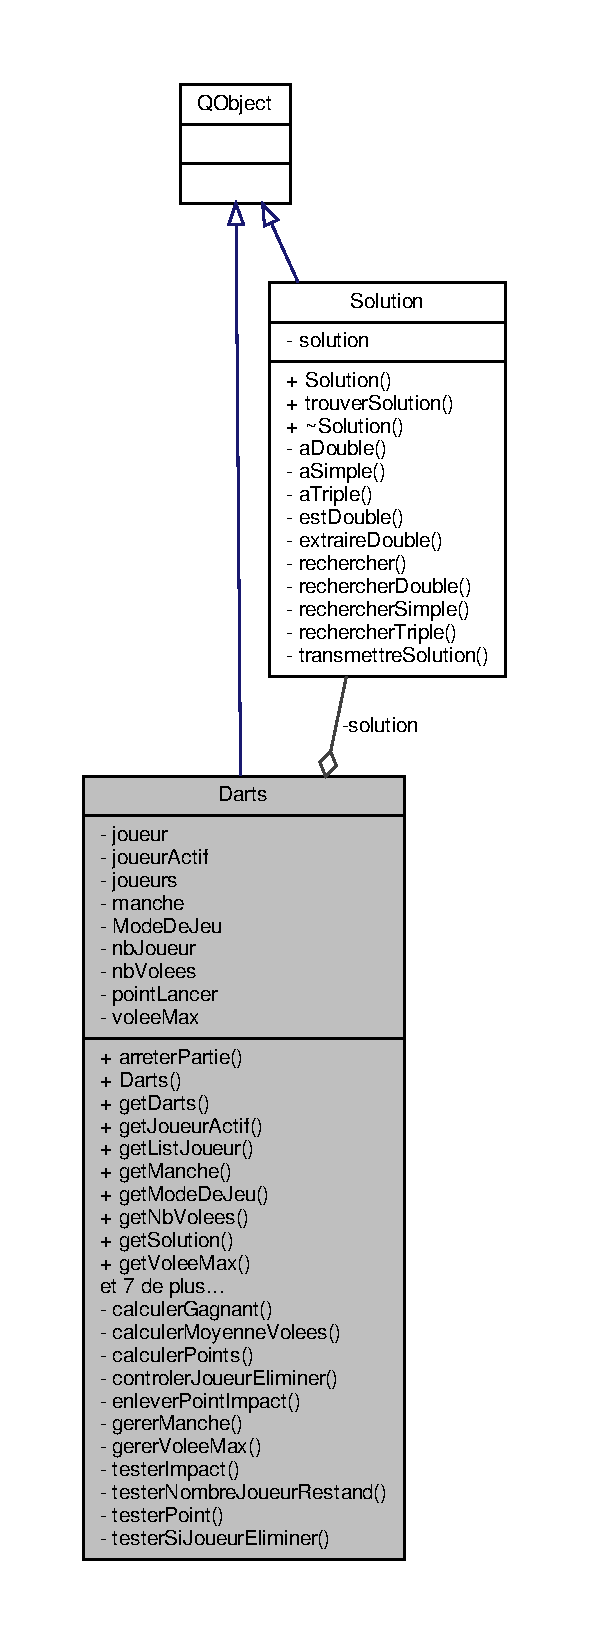
\includegraphics[height=550pt]{class_darts__coll__graph}
\end{center}
\end{figure}
\subsubsection*{Signaux}
\begin{DoxyCompactItemize}
\item 
void \hyperlink{class_darts_afcf6c21d8489e9cf1734458a23b518eb}{actualiser\+Cible} ()
\begin{DoxyCompactList}\small\item\em signal émis pour changer actualiser l\textquotesingle{}affichage de la cible \end{DoxyCompactList}\item 
void \hyperlink{class_darts_a650d6efdef25756bfbbacb0bb3549c43}{afficher\+Nouvelle\+Partie} ()
\begin{DoxyCompactList}\small\item\em signal émis quand il y a une nouvelle partie \end{DoxyCompactList}\item 
void \hyperlink{class_darts_afeba952f29a901b4ebac86cfc7a4733f}{changement\+Joueur\+Actif} ()
\begin{DoxyCompactList}\small\item\em signal émis quand le joueur actif change \end{DoxyCompactList}\item 
void \hyperlink{class_darts_a25cf64530c84d7aa261a4806e88dcd6e}{changer\+Etat\+Partie} ()
\begin{DoxyCompactList}\small\item\em signal émis pour changer l\textquotesingle{}etat de la partie \end{DoxyCompactList}\item 
void \hyperlink{class_darts_a04a60e25e4c6a608a15c6abce35c9dfa}{etat\+Partie\+Fini} ()
\begin{DoxyCompactList}\small\item\em signal émis pour mettre l\textquotesingle{}etat de la partie en fin \end{DoxyCompactList}\item 
void \hyperlink{class_darts_a751870924fe01a94fbf49ce45451a218}{fin\+Partie} (Q\+String, int)
\begin{DoxyCompactList}\small\item\em signal émis quand c\textquotesingle{}est la fin de la partie \end{DoxyCompactList}\item 
void \hyperlink{class_darts_a87995841c66fc321b63c28fa8a786347}{jouer\+Son} (Q\+String son)
\begin{DoxyCompactList}\small\item\em signal émis pour Lancer un son \end{DoxyCompactList}\item 
void \hyperlink{class_darts_a70c1ccef5cb7e47bff1384041ad9a596}{mise\+A\+Jour\+Moyenne\+Volee} ()
\begin{DoxyCompactList}\small\item\em signal émis pour mettre à jour la moyenne des volées \end{DoxyCompactList}\item 
void \hyperlink{class_darts_a455fa1efac223393aff2afbd33352569}{mise\+A\+Jour\+Point} ()
\begin{DoxyCompactList}\small\item\em signal émis pour mettre à jour les points des joueurs \end{DoxyCompactList}\item 
void \hyperlink{class_darts_aae5288e0c0f09a9837bcb7a517ede5af}{nouvel\+Impact} (int, int, int)
\begin{DoxyCompactList}\small\item\em signal émis quand il y a un nouvel Impact \end{DoxyCompactList}\item 
void \hyperlink{class_darts_ace3f99f5381399b0b86e5b8192d6fd71}{nouvelle\+Manche} ()
\begin{DoxyCompactList}\small\item\em signal émis quand on change de manche \end{DoxyCompactList}\item 
void \hyperlink{class_darts_a78f609ea9e8867459804bad777ce39f3}{volee\+Annulee} ()
\begin{DoxyCompactList}\small\item\em signal émis quand la volées est annulé \end{DoxyCompactList}\end{DoxyCompactItemize}
\subsubsection*{Fonctions membres publiques}
\begin{DoxyCompactItemize}
\item 
void \hyperlink{class_darts_aa9685f754172d995cdd04d39d9651227}{arreter\+Partie} ()
\begin{DoxyCompactList}\small\item\em arrête la partie \end{DoxyCompactList}\item 
\hyperlink{class_darts_aaa3365c94f97e58a61a05082d0d324d7}{Darts} (\hyperlink{class_q_object}{Q\+Object} $\ast$parent=nullptr)
\begin{DoxyCompactList}\small\item\em Constructeur de la classe \hyperlink{class_darts}{Darts}. \end{DoxyCompactList}\item 
\hyperlink{class_darts}{Darts} $\ast$ \hyperlink{class_darts_a6548d12f81017792cf46b25f68fc5df8}{get\+Darts} ()
\item 
int \hyperlink{class_darts_a20ddfd28c8355c06a90cc23abff3de11}{get\+Joueur\+Actif} ()
\begin{DoxyCompactList}\small\item\em Retourne le numéro du joueur actif. \end{DoxyCompactList}\item 
Q\+List$<$ \hyperlink{class_joueur}{Joueur} $>$ \hyperlink{class_darts_a0525b09703d3461bf5570197354743c3}{get\+List\+Joueur} () const
\begin{DoxyCompactList}\small\item\em Retourne une liste des joueurs. \end{DoxyCompactList}\item 
int \hyperlink{class_darts_a2ce03c887d90f3a997648981d342b50c}{get\+Manche} () const
\begin{DoxyCompactList}\small\item\em Retourne la manche. \end{DoxyCompactList}\item 
Q\+String \hyperlink{class_darts_a49ea4ca23fd03d80f5a95257c6fe8478}{get\+Mode\+De\+Jeu} ()
\begin{DoxyCompactList}\small\item\em Retourne le mode de jeu. \end{DoxyCompactList}\item 
int \hyperlink{class_darts_a4b93d786fbd25b9512ad08b67bca0a69}{get\+Nb\+Volees} ()
\begin{DoxyCompactList}\small\item\em Retourne le nombre de volées de la partie. \end{DoxyCompactList}\item 
\hyperlink{class_solution}{Solution} $\ast$ \hyperlink{class_darts_a2e41c247a12dfd3065c77c2484fc5532}{get\+Solution} () const
\begin{DoxyCompactList}\small\item\em retourne l\textquotesingle{}objet solution \end{DoxyCompactList}\item 
int \hyperlink{class_darts_af2ca14bafbcdabe87fc306cc2e1d390e}{get\+Volee\+Max} ()
\begin{DoxyCompactList}\small\item\em Retourne la volée max. \end{DoxyCompactList}\item 
void \hyperlink{class_darts_ac7000897b8d394c3be39804813a39dc8}{initialiser\+Partie} (Q\+String\+List joueur\+List, Q\+String mode\+Jeu)
\begin{DoxyCompactList}\small\item\em Initialise la partie. \end{DoxyCompactList}\item 
void \hyperlink{class_darts_a196bc4307c631310f641606012ab9e05}{receptionner\+Impact} (int type\+Point, int point)
\begin{DoxyCompactList}\small\item\em Permets de traiter la réception d\textquotesingle{}impact. \end{DoxyCompactList}\item 
void \hyperlink{class_darts_a70c68ed8bd56b63df203c25e6ed14f3b}{reinitialiser\+Partie} ()
\begin{DoxyCompactList}\small\item\em Méthode qui permet de remettre a zero les differents attribut et conteneur pour une nouvelle partie. \end{DoxyCompactList}\item 
void \hyperlink{class_darts_ab038eac80e5fc5e8abbab5682e87f8f2}{set\+Manche} (int \hyperlink{class_darts_ac7b7bd23e64b4fab3895f02f085ea85f}{manche})
\begin{DoxyCompactList}\small\item\em Permets de mettre à jour le numéro de manche. \end{DoxyCompactList}\item 
void \hyperlink{class_darts_a982dda6ea65e4ada297cc562617fc3ba}{set\+Volee\+Max} (int \hyperlink{class_darts_aed9c6aa8f34fb2dcbc57a5ea24aa6c2a}{volee\+Max})
\begin{DoxyCompactList}\small\item\em Permets de mettre à jour le volé max. \end{DoxyCompactList}\item 
Q\+String \hyperlink{class_darts_ad6535ce917119069ec099cea0e744971}{tester\+Mode\+De\+Jeu} ()
\begin{DoxyCompactList}\small\item\em Méthode qui teste le mode de jeu. \end{DoxyCompactList}\item 
\hyperlink{class_darts_a335882c9fccd527d5c33a509269e0997}{$\sim$\+Darts} ()
\begin{DoxyCompactList}\small\item\em Destructeur de la classe \hyperlink{class_darts}{Darts}. \end{DoxyCompactList}\end{DoxyCompactItemize}
\subsubsection*{Fonctions membres privées}
\begin{DoxyCompactItemize}
\item 
Q\+String \hyperlink{class_darts_a4d7196c95f584cdce4a33d52f934121f}{calculer\+Gagnant} ()
\begin{DoxyCompactList}\small\item\em Calcule le gagnant de la partie si la partie doit s\textquotesingle{}arrêter avant la fin. \end{DoxyCompactList}\item 
void \hyperlink{class_darts_af87b6a1cd30838b99379aa4061fc43cc}{calculer\+Moyenne\+Volees} ()
\begin{DoxyCompactList}\small\item\em Calcule la moyenne des volées de chaque joueur. \end{DoxyCompactList}\item 
void \hyperlink{class_darts_a6a6c58dee559e851709d76fef9a8c6da}{calculer\+Points} (int point, int type\+Point)
\begin{DoxyCompactList}\small\item\em Teste s\textquotesingle{}il reste qu\textquotesingle{}un joueur n\textquotesingle{}était pas éliminé \end{DoxyCompactList}\item 
void \hyperlink{class_darts_a4ddf889c9c3933e061b182aeb5680c20}{controler\+Joueur\+Eliminer} ()
\begin{DoxyCompactList}\small\item\em Change de joueur si le joueur actuel est éliminé \end{DoxyCompactList}\item 
void \hyperlink{class_darts_ac96311be89ac838f4a37b91bd5655171}{enlever\+Point\+Impact} ()
\begin{DoxyCompactList}\small\item\em Met à jours le score du joueur. \end{DoxyCompactList}\item 
void \hyperlink{class_darts_a76db114bd2191b410bab26cfe5cb76fb}{gerer\+Manche} ()
\begin{DoxyCompactList}\small\item\em Permets de gérer le changement de manche en fonction des fléchettes de chaque joueur. \end{DoxyCompactList}\item 
void \hyperlink{class_darts_a1bd32af08207f7465f2973821a25dbae}{gerer\+Volee\+Max} ()
\begin{DoxyCompactList}\small\item\em Teste la volée pour savoir si elle est supérieure à la volée Max. \end{DoxyCompactList}\item 
void \hyperlink{class_darts_af34338eccf367fb9ed939ff95768a221}{tester\+Impact} (int type\+Point)
\begin{DoxyCompactList}\small\item\em Teste si le joueur a gagné \end{DoxyCompactList}\item 
void \hyperlink{class_darts_a0fbfcd2202600e886177e2202a44b3bd}{tester\+Nombre\+Joueur\+Restand} ()
\begin{DoxyCompactList}\small\item\em Teste s\textquotesingle{}il reste qu\textquotesingle{}un joueur n\textquotesingle{}était pas éliminé \end{DoxyCompactList}\item 
void \hyperlink{class_darts_a7244911a7b1fe50023987a1c802a5103}{tester\+Point} (int type\+Point, int point)
\begin{DoxyCompactList}\small\item\em Méthode qui teste les Impact pour savoir quel son jouer. \end{DoxyCompactList}\item 
void \hyperlink{class_darts_a0b01c46befe8ee6c1c61b79b0fd817f8}{tester\+Si\+Joueur\+Eliminer} ()
\begin{DoxyCompactList}\small\item\em Teste si le joueur est à 1 point à la fin de la manche. \end{DoxyCompactList}\end{DoxyCompactItemize}
\subsubsection*{Attributs privés}
\begin{DoxyCompactItemize}
\item 
Q\+String\+List \hyperlink{class_darts_a97cc62d823c3d41604bb4a2d329ddfea}{joueur}
\begin{DoxyCompactList}\small\item\em contient les noms des differents joueur \end{DoxyCompactList}\item 
int \hyperlink{class_darts_a68fb01b9aad6502e4429dfbf2a72d50b}{joueur\+Actif}
\begin{DoxyCompactList}\small\item\em contient le numero du joueur en train de jouer \end{DoxyCompactList}\item 
Q\+List$<$ \hyperlink{class_joueur}{Joueur} $>$ \hyperlink{class_darts_a81bc116f3ae70cea1f492f87f01901c7}{joueurs}
\begin{DoxyCompactList}\small\item\em contient des objets joueurs \end{DoxyCompactList}\item 
int \hyperlink{class_darts_ac7b7bd23e64b4fab3895f02f085ea85f}{manche}
\begin{DoxyCompactList}\small\item\em contient le numero de la manche actuel \end{DoxyCompactList}\item 
Q\+String \hyperlink{class_darts_a281fd6201343dfb65ab81c93fd60f786}{Mode\+De\+Jeu}
\begin{DoxyCompactList}\small\item\em contient le mode de jeu en cours \end{DoxyCompactList}\item 
int \hyperlink{class_darts_ac5ae0e3546d00f59adba76c4ece71725}{nb\+Joueur}
\begin{DoxyCompactList}\small\item\em contient le nombre de joueur \end{DoxyCompactList}\item 
int \hyperlink{class_darts_ae73a0b876ca354c7abd0d39db15c94fa}{nb\+Volees}
\begin{DoxyCompactList}\small\item\em contient le nombre de Volées de la partie en cours \end{DoxyCompactList}\item 
int \hyperlink{class_darts_a7ed0e6c9c07930603f85c2bac5b9d78b}{point\+Lancer}
\begin{DoxyCompactList}\small\item\em contient les point associer l\textquotesingle{}impact de la fleche \end{DoxyCompactList}\item 
\hyperlink{class_solution}{Solution} $\ast$ \hyperlink{class_darts_a40733010dc6ae4ce93140804b4d191ea}{solution}
\begin{DoxyCompactList}\small\item\em Association vers l\textquotesingle{}objet solution. \end{DoxyCompactList}\item 
int \hyperlink{class_darts_aed9c6aa8f34fb2dcbc57a5ea24aa6c2a}{volee\+Max}
\begin{DoxyCompactList}\small\item\em contient la volées Max \end{DoxyCompactList}\end{DoxyCompactItemize}


\subsubsection{Description détaillée}
Déclaration de la classe \hyperlink{class_darts}{Darts} (Module Ecran-\/\+D\+A\+R\+TS) 

Cette classe s\textquotesingle{}occuper du déroulement d\textquotesingle{}une partie 

Définition à la ligne \hyperlink{darts_8h_source_l00032}{32} du fichier \hyperlink{darts_8h_source}{darts.\+h}.



\subsubsection{Documentation des constructeurs et destructeur}
\mbox{\Hypertarget{class_darts_aaa3365c94f97e58a61a05082d0d324d7}\label{class_darts_aaa3365c94f97e58a61a05082d0d324d7}} 
\index{Darts@{Darts}!Darts@{Darts}}
\index{Darts@{Darts}!Darts@{Darts}}
\paragraph{\texorpdfstring{Darts()}{Darts()}}
{\footnotesize\ttfamily Darts\+::\+Darts (\begin{DoxyParamCaption}\item[{\hyperlink{class_q_object}{Q\+Object} $\ast$}]{parent = {\ttfamily nullptr} }\end{DoxyParamCaption})\hspace{0.3cm}{\ttfamily [explicit]}}



Constructeur de la classe \hyperlink{class_darts}{Darts}. 


\begin{DoxyParams}{Paramètres}
{\em parent} & \\
\hline
\end{DoxyParams}


Définition à la ligne \hyperlink{darts_8cpp_source_l00022}{22} du fichier \hyperlink{darts_8cpp_source}{darts.\+cpp}.



Références \hyperlink{darts_8h_source_l00072}{solution}.


\begin{DoxyCode}
00022                             : \hyperlink{class_q_object}{QObject}(parent), \hyperlink{class_darts_a97cc62d823c3d41604bb4a2d329ddfea}{joueur}(\textcolor{keyword}{nullptr}), 
      \hyperlink{class_darts_ac5ae0e3546d00f59adba76c4ece71725}{nbJoueur}(0), \hyperlink{class_darts_a68fb01b9aad6502e4429dfbf2a72d50b}{joueurActif}(0), \hyperlink{class_darts_ac7b7bd23e64b4fab3895f02f085ea85f}{manche}(1), \hyperlink{class_darts_a7ed0e6c9c07930603f85c2bac5b9d78b}{pointLancer}(0), 
      \hyperlink{class_darts_aed9c6aa8f34fb2dcbc57a5ea24aa6c2a}{voleeMax}(0), \hyperlink{class_darts_ae73a0b876ca354c7abd0d39db15c94fa}{nbVolees}(0), \hyperlink{class_darts_a281fd6201343dfb65ab81c93fd60f786}{ModeDeJeu}(\textcolor{stringliteral}{""})
00023 \{
00024     qDebug() << Q\_FUNC\_INFO;
00025     \hyperlink{class_darts_a40733010dc6ae4ce93140804b4d191ea}{solution} = \textcolor{keyword}{new} \hyperlink{class_solution}{Solution}(\textcolor{keyword}{this});
00026 \}
\end{DoxyCode}
\mbox{\Hypertarget{class_darts_a335882c9fccd527d5c33a509269e0997}\label{class_darts_a335882c9fccd527d5c33a509269e0997}} 
\index{Darts@{Darts}!````~Darts@{$\sim$\+Darts}}
\index{````~Darts@{$\sim$\+Darts}!Darts@{Darts}}
\paragraph{\texorpdfstring{$\sim$\+Darts()}{~Darts()}}
{\footnotesize\ttfamily Darts\+::$\sim$\+Darts (\begin{DoxyParamCaption}{ }\end{DoxyParamCaption})}



Destructeur de la classe \hyperlink{class_darts}{Darts}. 



Définition à la ligne \hyperlink{darts_8cpp_source_l00033}{33} du fichier \hyperlink{darts_8cpp_source}{darts.\+cpp}.


\begin{DoxyCode}
00034 \{
00035     qDebug() << Q\_FUNC\_INFO;
00036 \}
\end{DoxyCode}


\subsubsection{Documentation des fonctions membres}
\mbox{\Hypertarget{class_darts_afcf6c21d8489e9cf1734458a23b518eb}\label{class_darts_afcf6c21d8489e9cf1734458a23b518eb}} 
\index{Darts@{Darts}!actualiser\+Cible@{actualiser\+Cible}}
\index{actualiser\+Cible@{actualiser\+Cible}!Darts@{Darts}}
\paragraph{\texorpdfstring{actualiser\+Cible}{actualiserCible}}
{\footnotesize\ttfamily void Darts\+::actualiser\+Cible (\begin{DoxyParamCaption}{ }\end{DoxyParamCaption})\hspace{0.3cm}{\ttfamily [signal]}}



signal émis pour changer actualiser l\textquotesingle{}affichage de la cible 



Référencé par \hyperlink{darts_8cpp_source_l00223}{receptionner\+Impact()}.

\mbox{\Hypertarget{class_darts_a650d6efdef25756bfbbacb0bb3549c43}\label{class_darts_a650d6efdef25756bfbbacb0bb3549c43}} 
\index{Darts@{Darts}!afficher\+Nouvelle\+Partie@{afficher\+Nouvelle\+Partie}}
\index{afficher\+Nouvelle\+Partie@{afficher\+Nouvelle\+Partie}!Darts@{Darts}}
\paragraph{\texorpdfstring{afficher\+Nouvelle\+Partie}{afficherNouvellePartie}}
{\footnotesize\ttfamily void Darts\+::afficher\+Nouvelle\+Partie (\begin{DoxyParamCaption}{ }\end{DoxyParamCaption})\hspace{0.3cm}{\ttfamily [signal]}}



signal émis quand il y a une nouvelle partie 



Référencé par \hyperlink{darts_8cpp_source_l00144}{initialiser\+Partie()}.

\mbox{\Hypertarget{class_darts_aa9685f754172d995cdd04d39d9651227}\label{class_darts_aa9685f754172d995cdd04d39d9651227}} 
\index{Darts@{Darts}!arreter\+Partie@{arreter\+Partie}}
\index{arreter\+Partie@{arreter\+Partie}!Darts@{Darts}}
\paragraph{\texorpdfstring{arreter\+Partie()}{arreterPartie()}}
{\footnotesize\ttfamily void Darts\+::arreter\+Partie (\begin{DoxyParamCaption}{ }\end{DoxyParamCaption})}



arrête la partie 



Définition à la ligne \hyperlink{darts_8cpp_source_l00422}{422} du fichier \hyperlink{darts_8cpp_source}{darts.\+cpp}.



Références \hyperlink{darts_8cpp_source_l00433}{calculer\+Gagnant()}, \hyperlink{class_darts_a751870924fe01a94fbf49ce45451a218}{fin\+Partie()}, et \hyperlink{darts_8cpp_source_l00066}{get\+Volee\+Max()}.



Référencé par \hyperlink{communication_8cpp_source_l00188}{Communication\+::decomposer\+Trame()}, et \hyperlink{darts_8cpp_source_l00453}{tester\+Nombre\+Joueur\+Restand()}.


\begin{DoxyCode}
00423 \{
00424     emit \hyperlink{class_darts_a751870924fe01a94fbf49ce45451a218}{finPartie}(\hyperlink{class_darts_a4d7196c95f584cdce4a33d52f934121f}{calculerGagnant}(), \hyperlink{class_darts_af2ca14bafbcdabe87fc306cc2e1d390e}{getVoleeMax}());
00425 \}
\end{DoxyCode}
\mbox{\Hypertarget{class_darts_a4d7196c95f584cdce4a33d52f934121f}\label{class_darts_a4d7196c95f584cdce4a33d52f934121f}} 
\index{Darts@{Darts}!calculer\+Gagnant@{calculer\+Gagnant}}
\index{calculer\+Gagnant@{calculer\+Gagnant}!Darts@{Darts}}
\paragraph{\texorpdfstring{calculer\+Gagnant()}{calculerGagnant()}}
{\footnotesize\ttfamily Q\+String Darts\+::calculer\+Gagnant (\begin{DoxyParamCaption}{ }\end{DoxyParamCaption})\hspace{0.3cm}{\ttfamily [private]}}



Calcule le gagnant de la partie si la partie doit s\textquotesingle{}arrêter avant la fin. 

\begin{DoxyReturn}{Renvoie}
Q\+String 
\end{DoxyReturn}


Définition à la ligne \hyperlink{darts_8cpp_source_l00433}{433} du fichier \hyperlink{darts_8cpp_source}{darts.\+cpp}.



Références \hyperlink{darts_8h_source_l00073}{joueurs}.



Référencé par \hyperlink{darts_8cpp_source_l00422}{arreter\+Partie()}.


\begin{DoxyCode}
00434 \{
00435     QString gagnant;
00436     \textcolor{keywordtype}{int} scoreGagnant = 99999;
00437     \textcolor{keywordflow}{for}(\textcolor{keywordtype}{int} i = 0; i <= \hyperlink{class_darts_a81bc116f3ae70cea1f492f87f01901c7}{joueurs}.size() - 1; i++)
00438     \{
00439         \textcolor{keywordflow}{if}(scoreGagnant > \hyperlink{class_darts_a81bc116f3ae70cea1f492f87f01901c7}{joueurs}[i].getScore() && !\hyperlink{class_darts_a81bc116f3ae70cea1f492f87f01901c7}{joueurs}[i].getEliminer()) \textcolor{comment}{// test le
       personne aillant le score le plus bas score mais aussi qu'il ne soit pas eliminer}
00440         \{
00441             scoreGagnant = \hyperlink{class_darts_a81bc116f3ae70cea1f492f87f01901c7}{joueurs}[i].getScore();
00442             gagnant = \hyperlink{class_darts_a81bc116f3ae70cea1f492f87f01901c7}{joueurs}[i].getNom();
00443         \}
00444     \}
00445     \textcolor{keywordflow}{return} \textcolor{stringliteral}{"↢  Winner "} + gagnant + \textcolor{stringliteral}{"  ↣"};
00446 \}
\end{DoxyCode}
\mbox{\Hypertarget{class_darts_af87b6a1cd30838b99379aa4061fc43cc}\label{class_darts_af87b6a1cd30838b99379aa4061fc43cc}} 
\index{Darts@{Darts}!calculer\+Moyenne\+Volees@{calculer\+Moyenne\+Volees}}
\index{calculer\+Moyenne\+Volees@{calculer\+Moyenne\+Volees}!Darts@{Darts}}
\paragraph{\texorpdfstring{calculer\+Moyenne\+Volees()}{calculerMoyenneVolees()}}
{\footnotesize\ttfamily void Darts\+::calculer\+Moyenne\+Volees (\begin{DoxyParamCaption}{ }\end{DoxyParamCaption})\hspace{0.3cm}{\ttfamily [private]}}



Calcule la moyenne des volées de chaque joueur. 



Définition à la ligne \hyperlink{darts_8cpp_source_l00387}{387} du fichier \hyperlink{darts_8cpp_source}{darts.\+cpp}.



Références \hyperlink{darts_8h_source_l00073}{joueurs}, et \hyperlink{class_darts_a70c1ccef5cb7e47bff1384041ad9a596}{mise\+A\+Jour\+Moyenne\+Volee()}.



Référencé par \hyperlink{darts_8cpp_source_l00349}{controler\+Joueur\+Eliminer()}, et \hyperlink{darts_8cpp_source_l00303}{gerer\+Manche()}.


\begin{DoxyCode}
00388 \{
00389     \textcolor{keywordflow}{for}(\textcolor{keywordtype}{int} i = 0; i <= \hyperlink{class_darts_a81bc116f3ae70cea1f492f87f01901c7}{joueurs}.size() - 1; i++)
00390     \{
00391         \textcolor{keywordtype}{int} moyenneVolee = 0;
00392 
00393         \textcolor{keywordflow}{for}(\textcolor{keywordtype}{int} j = 0; j < \hyperlink{class_darts_a81bc116f3ae70cea1f492f87f01901c7}{joueurs}[i].getHistoriqueVolees().size(); j++)
00394         \{
00395             moyenneVolee += \hyperlink{class_darts_a81bc116f3ae70cea1f492f87f01901c7}{joueurs}[i].getHistoriqueVolees()[j];
00396         \}
00397 
00398         moyenneVolee = moyenneVolee / \hyperlink{class_darts_a81bc116f3ae70cea1f492f87f01901c7}{joueurs}[i].getHistoriqueVolees().size();
00399         \hyperlink{class_darts_a81bc116f3ae70cea1f492f87f01901c7}{joueurs}[i].setMoyenneVolee(moyenneVolee);
00400     \}
00401     emit \hyperlink{class_darts_a70c1ccef5cb7e47bff1384041ad9a596}{miseAJourMoyenneVolee}();
00402 \}
\end{DoxyCode}
\mbox{\Hypertarget{class_darts_a6a6c58dee559e851709d76fef9a8c6da}\label{class_darts_a6a6c58dee559e851709d76fef9a8c6da}} 
\index{Darts@{Darts}!calculer\+Points@{calculer\+Points}}
\index{calculer\+Points@{calculer\+Points}!Darts@{Darts}}
\paragraph{\texorpdfstring{calculer\+Points()}{calculerPoints()}}
{\footnotesize\ttfamily void Darts\+::calculer\+Points (\begin{DoxyParamCaption}\item[{int}]{point,  }\item[{int}]{type\+Point }\end{DoxyParamCaption})\hspace{0.3cm}{\ttfamily [private]}}



Teste s\textquotesingle{}il reste qu\textquotesingle{}un joueur n\textquotesingle{}était pas éliminé 


\begin{DoxyParams}{Paramètres}
{\em point} & la zone \\
\hline
{\em type\+Point} & un simple, double ou triple \\
\hline
\end{DoxyParams}


Définition à la ligne \hyperlink{darts_8cpp_source_l00478}{478} du fichier \hyperlink{darts_8cpp_source}{darts.\+cpp}.



Références \hyperlink{darts_8h_source_l00019}{D\+O\+U\+B\+L\+E\+\_\+\+P\+O\+I\+NT}, \hyperlink{darts_8h_source_l00078}{point\+Lancer}, \hyperlink{darts_8h_source_l00020}{S\+I\+M\+P\+L\+E\+\_\+\+P\+O\+I\+NT}, \hyperlink{darts_8h_source_l00018}{T\+R\+I\+P\+L\+E\+\_\+\+P\+O\+I\+NT}, et \hyperlink{darts_8h_source_l00021}{Z\+E\+R\+O\+\_\+\+P\+O\+I\+NT}.



Référencé par \hyperlink{darts_8cpp_source_l00223}{receptionner\+Impact()}.


\begin{DoxyCode}
00479 \{
00480     \textcolor{keywordflow}{switch}(typePoint)
00481     \{
00482         \textcolor{keywordflow}{case} \hyperlink{darts_8h_a1bd6caead3e7edd423f064b3af34e486}{TRIPLE\_POINT}:
00483             \hyperlink{class_darts_a7ed0e6c9c07930603f85c2bac5b9d78b}{pointLancer} = point * \hyperlink{darts_8h_a1bd6caead3e7edd423f064b3af34e486}{TRIPLE\_POINT};
00484         \textcolor{keywordflow}{break};
00485         \textcolor{keywordflow}{case} \hyperlink{darts_8h_af67ad443603f4dddf225d062757614ca}{DOUBLE\_POINT}:
00486             \hyperlink{class_darts_a7ed0e6c9c07930603f85c2bac5b9d78b}{pointLancer} = point * \hyperlink{darts_8h_af67ad443603f4dddf225d062757614ca}{DOUBLE\_POINT};
00487         \textcolor{keywordflow}{break};
00488         \textcolor{keywordflow}{case} \hyperlink{darts_8h_a180cfdf433b8c9594f209d3c71c7c992}{SIMPLE\_POINT}:
00489             \hyperlink{class_darts_a7ed0e6c9c07930603f85c2bac5b9d78b}{pointLancer} = point;
00490         \textcolor{keywordflow}{break};
00491         \textcolor{keywordflow}{case}  \hyperlink{darts_8h_a02bea0ce22b1e13c5065f434182317fb}{ZERO\_POINT}:
00492             \hyperlink{class_darts_a7ed0e6c9c07930603f85c2bac5b9d78b}{pointLancer} = point * \hyperlink{darts_8h_a02bea0ce22b1e13c5065f434182317fb}{ZERO\_POINT};
00493         \textcolor{keywordflow}{break};
00494         \textcolor{keywordflow}{default}:
00495             qDebug() << Q\_FUNC\_INFO << \textcolor{stringliteral}{"type de point non valide:"} << typePoint;
00496         \textcolor{keywordflow}{break};
00497     \}
00498 \}
\end{DoxyCode}
\mbox{\Hypertarget{class_darts_afeba952f29a901b4ebac86cfc7a4733f}\label{class_darts_afeba952f29a901b4ebac86cfc7a4733f}} 
\index{Darts@{Darts}!changement\+Joueur\+Actif@{changement\+Joueur\+Actif}}
\index{changement\+Joueur\+Actif@{changement\+Joueur\+Actif}!Darts@{Darts}}
\paragraph{\texorpdfstring{changement\+Joueur\+Actif}{changementJoueurActif}}
{\footnotesize\ttfamily void Darts\+::changement\+Joueur\+Actif (\begin{DoxyParamCaption}{ }\end{DoxyParamCaption})\hspace{0.3cm}{\ttfamily [signal]}}



signal émis quand le joueur actif change 



Référencé par \hyperlink{darts_8cpp_source_l00303}{gerer\+Manche()}.

\mbox{\Hypertarget{class_darts_a25cf64530c84d7aa261a4806e88dcd6e}\label{class_darts_a25cf64530c84d7aa261a4806e88dcd6e}} 
\index{Darts@{Darts}!changer\+Etat\+Partie@{changer\+Etat\+Partie}}
\index{changer\+Etat\+Partie@{changer\+Etat\+Partie}!Darts@{Darts}}
\paragraph{\texorpdfstring{changer\+Etat\+Partie}{changerEtatPartie}}
{\footnotesize\ttfamily void Darts\+::changer\+Etat\+Partie (\begin{DoxyParamCaption}{ }\end{DoxyParamCaption})\hspace{0.3cm}{\ttfamily [signal]}}



signal émis pour changer l\textquotesingle{}etat de la partie 



Référencé par \hyperlink{darts_8cpp_source_l00144}{initialiser\+Partie()}.

\mbox{\Hypertarget{class_darts_a4ddf889c9c3933e061b182aeb5680c20}\label{class_darts_a4ddf889c9c3933e061b182aeb5680c20}} 
\index{Darts@{Darts}!controler\+Joueur\+Eliminer@{controler\+Joueur\+Eliminer}}
\index{controler\+Joueur\+Eliminer@{controler\+Joueur\+Eliminer}!Darts@{Darts}}
\paragraph{\texorpdfstring{controler\+Joueur\+Eliminer()}{controlerJoueurEliminer()}}
{\footnotesize\ttfamily void Darts\+::controler\+Joueur\+Eliminer (\begin{DoxyParamCaption}{ }\end{DoxyParamCaption})\hspace{0.3cm}{\ttfamily [private]}}



Change de joueur si le joueur actuel est éliminé 



Définition à la ligne \hyperlink{darts_8cpp_source_l00349}{349} du fichier \hyperlink{darts_8cpp_source}{darts.\+cpp}.



Références \hyperlink{darts_8cpp_source_l00387}{calculer\+Moyenne\+Volees()}, \hyperlink{darts_8cpp_source_l00044}{get\+Manche()}, \hyperlink{darts_8h_source_l00076}{joueur\+Actif}, \hyperlink{darts_8h_source_l00073}{joueurs}, \hyperlink{darts_8h_source_l00075}{nb\+Joueur}, \hyperlink{class_darts_ace3f99f5381399b0b86e5b8192d6fd71}{nouvelle\+Manche()}, et \hyperlink{darts_8cpp_source_l00132}{set\+Manche()}.



Référencé par \hyperlink{darts_8cpp_source_l00303}{gerer\+Manche()}.


\begin{DoxyCode}
00350 \{
00351     \textcolor{keywordflow}{while}(\hyperlink{class_darts_a81bc116f3ae70cea1f492f87f01901c7}{joueurs}[\hyperlink{class_darts_a68fb01b9aad6502e4429dfbf2a72d50b}{joueurActif}].getEliminer()) \textcolor{comment}{//tant que le joueur est eliminer on passe
       donc au joueur suivant}
00352     \{
00353         \textcolor{keywordflow}{if}(\hyperlink{class_darts_a68fb01b9aad6502e4429dfbf2a72d50b}{joueurActif} == \hyperlink{class_darts_ac5ae0e3546d00f59adba76c4ece71725}{nbJoueur} - 1)  \textcolor{comment}{//si le joueur est le dernier de la manche à
       jouer}
00354         \{
00355             \hyperlink{class_darts_a68fb01b9aad6502e4429dfbf2a72d50b}{joueurActif} = 0;
00356             \hyperlink{class_darts_ab038eac80e5fc5e8abbab5682e87f8f2}{setManche}(\hyperlink{class_darts_a2ce03c887d90f3a997648981d342b50c}{getManche}() + 1);
00357             \hyperlink{class_darts_af87b6a1cd30838b99379aa4061fc43cc}{calculerMoyenneVolees}();
00358             emit \hyperlink{class_darts_ace3f99f5381399b0b86e5b8192d6fd71}{nouvelleManche}();
00359         \}
00360         \textcolor{keywordflow}{else}                            \textcolor{comment}{//si le joueur n'est pas le dernier de la manche}
00361         \{
00362             \hyperlink{class_darts_a68fb01b9aad6502e4429dfbf2a72d50b}{joueurActif}++;
00363         \}
00364     \}
00365 \}
\end{DoxyCode}
\mbox{\Hypertarget{class_darts_ac96311be89ac838f4a37b91bd5655171}\label{class_darts_ac96311be89ac838f4a37b91bd5655171}} 
\index{Darts@{Darts}!enlever\+Point\+Impact@{enlever\+Point\+Impact}}
\index{enlever\+Point\+Impact@{enlever\+Point\+Impact}!Darts@{Darts}}
\paragraph{\texorpdfstring{enlever\+Point\+Impact()}{enleverPointImpact()}}
{\footnotesize\ttfamily void Darts\+::enlever\+Point\+Impact (\begin{DoxyParamCaption}{ }\end{DoxyParamCaption})\hspace{0.3cm}{\ttfamily [private]}}



Met à jours le score du joueur. 



Définition à la ligne \hyperlink{darts_8cpp_source_l00274}{274} du fichier \hyperlink{darts_8cpp_source}{darts.\+cpp}.



Références \hyperlink{class_darts_a04a60e25e4c6a608a15c6abce35c9dfa}{etat\+Partie\+Fini()}, \hyperlink{class_darts_a751870924fe01a94fbf49ce45451a218}{fin\+Partie()}, \hyperlink{darts_8cpp_source_l00409}{gerer\+Volee\+Max()}, \hyperlink{darts_8cpp_source_l00066}{get\+Volee\+Max()}, \hyperlink{class_darts_a87995841c66fc321b63c28fa8a786347}{jouer\+Son()}, \hyperlink{darts_8h_source_l00076}{joueur\+Actif}, \hyperlink{darts_8h_source_l00073}{joueurs}, \hyperlink{darts_8h_source_l00080}{nb\+Volees}, \hyperlink{darts_8h_source_l00072}{solution}, \hyperlink{solution_8cpp_source_l00296}{Solution\+::trouver\+Solution()}, et \hyperlink{class_darts_a78f609ea9e8867459804bad777ce39f3}{volee\+Annulee()}.



Référencé par \hyperlink{darts_8cpp_source_l00246}{tester\+Impact()}.


\begin{DoxyCode}
00275 \{
00276     \textcolor{keywordflow}{if}(\hyperlink{class_darts_a81bc116f3ae70cea1f492f87f01901c7}{joueurs}[\hyperlink{class_darts_a68fb01b9aad6502e4429dfbf2a72d50b}{joueurActif}].getScore() <= 0) \textcolor{comment}{//score Volée inferieure au score = Volée
       annulée}
00277     \{
00278         \hyperlink{class_darts_a81bc116f3ae70cea1f492f87f01901c7}{joueurs}[\hyperlink{class_darts_a68fb01b9aad6502e4429dfbf2a72d50b}{joueurActif}].setScore(\hyperlink{class_darts_a81bc116f3ae70cea1f492f87f01901c7}{joueurs}[
      \hyperlink{class_darts_a68fb01b9aad6502e4429dfbf2a72d50b}{joueurActif}].getScoreManchePrecedente());
00279         emit \hyperlink{class_darts_a78f609ea9e8867459804bad777ce39f3}{voleeAnnulee}();
00280 
00281         \hyperlink{class_darts_a81bc116f3ae70cea1f492f87f01901c7}{joueurs}[\hyperlink{class_darts_a68fb01b9aad6502e4429dfbf2a72d50b}{joueurActif}].setNbFlechette(0);
00282     \}
00283     \textcolor{keywordflow}{else} \textcolor{keywordflow}{if}(\hyperlink{class_darts_a81bc116f3ae70cea1f492f87f01901c7}{joueurs}[\hyperlink{class_darts_a68fb01b9aad6502e4429dfbf2a72d50b}{joueurActif}].getScore() == 1 && \hyperlink{class_darts_a81bc116f3ae70cea1f492f87f01901c7}{joueurs}.size() == 1)    \textcolor{comment}{//
       test si le joueur est seul à jouer et s'il est a 1 point == joueur éliminer donc fin de partie}
00284     \{
00285         \hyperlink{class_darts_a1bd32af08207f7465f2973821a25dbae}{gererVoleeMax}();
00286         emit \hyperlink{class_darts_a87995841c66fc321b63c28fa8a786347}{jouerSon}(\textcolor{stringliteral}{"perdu.wav"});
00287         emit \hyperlink{class_darts_a751870924fe01a94fbf49ce45451a218}{finPartie}(\textcolor{stringliteral}{"↢  "} + \hyperlink{class_darts_a81bc116f3ae70cea1f492f87f01901c7}{joueurs}[\hyperlink{class_darts_a68fb01b9aad6502e4429dfbf2a72d50b}{joueurActif}].getNom() + \textcolor{stringliteral}{" a perdu  ↣"}, 
      \hyperlink{class_darts_af2ca14bafbcdabe87fc306cc2e1d390e}{getVoleeMax}());
00288         emit \hyperlink{class_darts_a04a60e25e4c6a608a15c6abce35c9dfa}{etatPartieFini}();
00289     \}
00290     \textcolor{keywordflow}{else}
00291     \{
00292         \hyperlink{class_darts_ae73a0b876ca354c7abd0d39db15c94fa}{nbVolees}++;
00293         \hyperlink{class_darts_a81bc116f3ae70cea1f492f87f01901c7}{joueurs}[\hyperlink{class_darts_a68fb01b9aad6502e4429dfbf2a72d50b}{joueurActif}].setNbFlechette(\hyperlink{class_darts_a81bc116f3ae70cea1f492f87f01901c7}{joueurs}[
      \hyperlink{class_darts_a68fb01b9aad6502e4429dfbf2a72d50b}{joueurActif}].getFlechette() - 1);
00294         \hyperlink{class_darts_a40733010dc6ae4ce93140804b4d191ea}{solution}->\hyperlink{class_solution_a9ab0b0fd2b557f5abda8bd1a6da641e4}{trouverSolution}(\hyperlink{class_darts_a81bc116f3ae70cea1f492f87f01901c7}{joueurs}[
      \hyperlink{class_darts_a68fb01b9aad6502e4429dfbf2a72d50b}{joueurActif}].getScore(),\hyperlink{class_darts_a81bc116f3ae70cea1f492f87f01901c7}{joueurs}[\hyperlink{class_darts_a68fb01b9aad6502e4429dfbf2a72d50b}{joueurActif}].getFlechette());
00295     \}
00296 \}
\end{DoxyCode}
\mbox{\Hypertarget{class_darts_a04a60e25e4c6a608a15c6abce35c9dfa}\label{class_darts_a04a60e25e4c6a608a15c6abce35c9dfa}} 
\index{Darts@{Darts}!etat\+Partie\+Fini@{etat\+Partie\+Fini}}
\index{etat\+Partie\+Fini@{etat\+Partie\+Fini}!Darts@{Darts}}
\paragraph{\texorpdfstring{etat\+Partie\+Fini}{etatPartieFini}}
{\footnotesize\ttfamily void Darts\+::etat\+Partie\+Fini (\begin{DoxyParamCaption}{ }\end{DoxyParamCaption})\hspace{0.3cm}{\ttfamily [signal]}}



signal émis pour mettre l\textquotesingle{}etat de la partie en fin 



Référencé par \hyperlink{darts_8cpp_source_l00274}{enlever\+Point\+Impact()}, et \hyperlink{darts_8cpp_source_l00246}{tester\+Impact()}.

\mbox{\Hypertarget{class_darts_a751870924fe01a94fbf49ce45451a218}\label{class_darts_a751870924fe01a94fbf49ce45451a218}} 
\index{Darts@{Darts}!fin\+Partie@{fin\+Partie}}
\index{fin\+Partie@{fin\+Partie}!Darts@{Darts}}
\paragraph{\texorpdfstring{fin\+Partie}{finPartie}}
{\footnotesize\ttfamily void Darts\+::fin\+Partie (\begin{DoxyParamCaption}\item[{Q\+String}]{,  }\item[{int}]{ }\end{DoxyParamCaption})\hspace{0.3cm}{\ttfamily [signal]}}



signal émis quand c\textquotesingle{}est la fin de la partie 



Référencé par \hyperlink{darts_8cpp_source_l00422}{arreter\+Partie()}, \hyperlink{darts_8cpp_source_l00274}{enlever\+Point\+Impact()}, et \hyperlink{darts_8cpp_source_l00246}{tester\+Impact()}.

\mbox{\Hypertarget{class_darts_a76db114bd2191b410bab26cfe5cb76fb}\label{class_darts_a76db114bd2191b410bab26cfe5cb76fb}} 
\index{Darts@{Darts}!gerer\+Manche@{gerer\+Manche}}
\index{gerer\+Manche@{gerer\+Manche}!Darts@{Darts}}
\paragraph{\texorpdfstring{gerer\+Manche()}{gererManche()}}
{\footnotesize\ttfamily void Darts\+::gerer\+Manche (\begin{DoxyParamCaption}{ }\end{DoxyParamCaption})\hspace{0.3cm}{\ttfamily [private]}}



Permets de gérer le changement de manche en fonction des fléchettes de chaque joueur. 



Définition à la ligne \hyperlink{darts_8cpp_source_l00303}{303} du fichier \hyperlink{darts_8cpp_source}{darts.\+cpp}.



Références \hyperlink{darts_8cpp_source_l00387}{calculer\+Moyenne\+Volees()}, \hyperlink{class_darts_afeba952f29a901b4ebac86cfc7a4733f}{changement\+Joueur\+Actif()}, \hyperlink{darts_8cpp_source_l00349}{controler\+Joueur\+Eliminer()}, \hyperlink{darts_8cpp_source_l00409}{gerer\+Volee\+Max()}, \hyperlink{darts_8cpp_source_l00044}{get\+Manche()}, \hyperlink{class_darts_a87995841c66fc321b63c28fa8a786347}{jouer\+Son()}, \hyperlink{darts_8h_source_l00076}{joueur\+Actif}, \hyperlink{darts_8h_source_l00073}{joueurs}, \hyperlink{darts_8h_source_l00075}{nb\+Joueur}, \hyperlink{class_darts_ace3f99f5381399b0b86e5b8192d6fd71}{nouvelle\+Manche()}, \hyperlink{darts_8cpp_source_l00132}{set\+Manche()}, \hyperlink{darts_8h_source_l00072}{solution}, \hyperlink{darts_8cpp_source_l00453}{tester\+Nombre\+Joueur\+Restand()}, \hyperlink{darts_8cpp_source_l00372}{tester\+Si\+Joueur\+Eliminer()}, et \hyperlink{solution_8cpp_source_l00296}{Solution\+::trouver\+Solution()}.



Référencé par \hyperlink{darts_8cpp_source_l00246}{tester\+Impact()}.


\begin{DoxyCode}
00304 \{
00305     \textcolor{keywordflow}{if}(\hyperlink{class_darts_a81bc116f3ae70cea1f492f87f01901c7}{joueurs}[\hyperlink{class_darts_a68fb01b9aad6502e4429dfbf2a72d50b}{joueurActif}].getFlechette() == 0) \textcolor{comment}{//fin de la volées du joueur}
00306     \{
00307         \hyperlink{class_darts_a81bc116f3ae70cea1f492f87f01901c7}{joueurs}[\hyperlink{class_darts_a68fb01b9aad6502e4429dfbf2a72d50b}{joueurActif}].setNbFlechette(3);
00308 
00309         \hyperlink{class_darts_a1bd32af08207f7465f2973821a25dbae}{gererVoleeMax}();
00310         \hyperlink{class_darts_a0b01c46befe8ee6c1c61b79b0fd817f8}{testerSiJoueurEliminer}();
00311         \hyperlink{class_darts_a0fbfcd2202600e886177e2202a44b3bd}{testerNombreJoueurRestand}();
00312 
00313         \hyperlink{class_darts_a81bc116f3ae70cea1f492f87f01901c7}{joueurs}[\hyperlink{class_darts_a68fb01b9aad6502e4429dfbf2a72d50b}{joueurActif}].addHistoriqueVolees((\hyperlink{class_darts_a81bc116f3ae70cea1f492f87f01901c7}{joueurs}[
      \hyperlink{class_darts_a68fb01b9aad6502e4429dfbf2a72d50b}{joueurActif}].getScoreManchePrecedente() - \hyperlink{class_darts_a81bc116f3ae70cea1f492f87f01901c7}{joueurs}[\hyperlink{class_darts_a68fb01b9aad6502e4429dfbf2a72d50b}{joueurActif}].getScore()));
00314 
00315         \textcolor{keywordflow}{if}((\hyperlink{class_darts_a81bc116f3ae70cea1f492f87f01901c7}{joueurs}[\hyperlink{class_darts_a68fb01b9aad6502e4429dfbf2a72d50b}{joueurActif}].getScoreManchePrecedente() - 
      \hyperlink{class_darts_a81bc116f3ae70cea1f492f87f01901c7}{joueurs}[\hyperlink{class_darts_a68fb01b9aad6502e4429dfbf2a72d50b}{joueurActif}].getScore()) == 180)
00316             emit \hyperlink{class_darts_a87995841c66fc321b63c28fa8a786347}{jouerSon}(\textcolor{stringliteral}{"180.wav"});
00317 
00318         \hyperlink{class_darts_a81bc116f3ae70cea1f492f87f01901c7}{joueurs}[\hyperlink{class_darts_a68fb01b9aad6502e4429dfbf2a72d50b}{joueurActif}].setScoreManchePrecedente(\hyperlink{class_darts_a81bc116f3ae70cea1f492f87f01901c7}{joueurs}[
      \hyperlink{class_darts_a68fb01b9aad6502e4429dfbf2a72d50b}{joueurActif}].getScore());
00319 
00320         \textcolor{keywordflow}{if}(\hyperlink{class_darts_a68fb01b9aad6502e4429dfbf2a72d50b}{joueurActif} == \hyperlink{class_darts_ac5ae0e3546d00f59adba76c4ece71725}{nbJoueur} - 1)  \textcolor{comment}{//equivalent a la fin de manche}
00321         \{
00322             \hyperlink{class_darts_a68fb01b9aad6502e4429dfbf2a72d50b}{joueurActif} = 0;
00323 
00324             \hyperlink{class_darts_a4ddf889c9c3933e061b182aeb5680c20}{controlerJoueurEliminer}();
00325 
00326             \hyperlink{class_darts_ab038eac80e5fc5e8abbab5682e87f8f2}{setManche}(\hyperlink{class_darts_a2ce03c887d90f3a997648981d342b50c}{getManche}() + 1);
00327             emit \hyperlink{class_darts_afeba952f29a901b4ebac86cfc7a4733f}{changementJoueurActif}();
00328             \hyperlink{class_darts_af87b6a1cd30838b99379aa4061fc43cc}{calculerMoyenneVolees}();
00329             emit \hyperlink{class_darts_ace3f99f5381399b0b86e5b8192d6fd71}{nouvelleManche}();
00330             \hyperlink{class_darts_a40733010dc6ae4ce93140804b4d191ea}{solution}->\hyperlink{class_solution_a9ab0b0fd2b557f5abda8bd1a6da641e4}{trouverSolution}(\hyperlink{class_darts_a81bc116f3ae70cea1f492f87f01901c7}{joueurs}[
      \hyperlink{class_darts_a68fb01b9aad6502e4429dfbf2a72d50b}{joueurActif}].getScore(),\hyperlink{class_darts_a81bc116f3ae70cea1f492f87f01901c7}{joueurs}[\hyperlink{class_darts_a68fb01b9aad6502e4429dfbf2a72d50b}{joueurActif}].getFlechette());
00331         \}
00332         \textcolor{keywordflow}{else}
00333         \{
00334             \hyperlink{class_darts_a68fb01b9aad6502e4429dfbf2a72d50b}{joueurActif}++;
00335 
00336             \hyperlink{class_darts_a4ddf889c9c3933e061b182aeb5680c20}{controlerJoueurEliminer}();
00337 
00338             emit \hyperlink{class_darts_afeba952f29a901b4ebac86cfc7a4733f}{changementJoueurActif}();
00339             \hyperlink{class_darts_a40733010dc6ae4ce93140804b4d191ea}{solution}->\hyperlink{class_solution_a9ab0b0fd2b557f5abda8bd1a6da641e4}{trouverSolution}(\hyperlink{class_darts_a81bc116f3ae70cea1f492f87f01901c7}{joueurs}[
      \hyperlink{class_darts_a68fb01b9aad6502e4429dfbf2a72d50b}{joueurActif}].getScore(),\hyperlink{class_darts_a81bc116f3ae70cea1f492f87f01901c7}{joueurs}[\hyperlink{class_darts_a68fb01b9aad6502e4429dfbf2a72d50b}{joueurActif}].getFlechette());
00340         \}
00341     \}
00342 \}
\end{DoxyCode}
\mbox{\Hypertarget{class_darts_a1bd32af08207f7465f2973821a25dbae}\label{class_darts_a1bd32af08207f7465f2973821a25dbae}} 
\index{Darts@{Darts}!gerer\+Volee\+Max@{gerer\+Volee\+Max}}
\index{gerer\+Volee\+Max@{gerer\+Volee\+Max}!Darts@{Darts}}
\paragraph{\texorpdfstring{gerer\+Volee\+Max()}{gererVoleeMax()}}
{\footnotesize\ttfamily void Darts\+::gerer\+Volee\+Max (\begin{DoxyParamCaption}{ }\end{DoxyParamCaption})\hspace{0.3cm}{\ttfamily [private]}}



Teste la volée pour savoir si elle est supérieure à la volée Max. 



Définition à la ligne \hyperlink{darts_8cpp_source_l00409}{409} du fichier \hyperlink{darts_8cpp_source}{darts.\+cpp}.



Références \hyperlink{darts_8cpp_source_l00066}{get\+Volee\+Max()}, \hyperlink{darts_8h_source_l00076}{joueur\+Actif}, \hyperlink{darts_8h_source_l00073}{joueurs}, et \hyperlink{darts_8cpp_source_l00121}{set\+Volee\+Max()}.



Référencé par \hyperlink{darts_8cpp_source_l00274}{enlever\+Point\+Impact()}, \hyperlink{darts_8cpp_source_l00303}{gerer\+Manche()}, et \hyperlink{darts_8cpp_source_l00246}{tester\+Impact()}.


\begin{DoxyCode}
00410 \{
00411     \textcolor{keywordflow}{if}((\hyperlink{class_darts_a81bc116f3ae70cea1f492f87f01901c7}{joueurs}[\hyperlink{class_darts_a68fb01b9aad6502e4429dfbf2a72d50b}{joueurActif}].getScoreManchePrecedente() - 
      \hyperlink{class_darts_a81bc116f3ae70cea1f492f87f01901c7}{joueurs}[\hyperlink{class_darts_a68fb01b9aad6502e4429dfbf2a72d50b}{joueurActif}].getScore()) > \hyperlink{class_darts_af2ca14bafbcdabe87fc306cc2e1d390e}{getVoleeMax}())
00412     \{
00413         \hyperlink{class_darts_a982dda6ea65e4ada297cc562617fc3ba}{setVoleeMax}(\hyperlink{class_darts_a81bc116f3ae70cea1f492f87f01901c7}{joueurs}[\hyperlink{class_darts_a68fb01b9aad6502e4429dfbf2a72d50b}{joueurActif}].getScoreManchePrecedente() - 
      \hyperlink{class_darts_a81bc116f3ae70cea1f492f87f01901c7}{joueurs}[\hyperlink{class_darts_a68fb01b9aad6502e4429dfbf2a72d50b}{joueurActif}].getScore());
00414     \}
00415 \}
\end{DoxyCode}
\mbox{\Hypertarget{class_darts_a6548d12f81017792cf46b25f68fc5df8}\label{class_darts_a6548d12f81017792cf46b25f68fc5df8}} 
\index{Darts@{Darts}!get\+Darts@{get\+Darts}}
\index{get\+Darts@{get\+Darts}!Darts@{Darts}}
\paragraph{\texorpdfstring{get\+Darts()}{getDarts()}}
{\footnotesize\ttfamily \hyperlink{class_darts}{Darts}$\ast$ Darts\+::get\+Darts (\begin{DoxyParamCaption}{ }\end{DoxyParamCaption})}

\mbox{\Hypertarget{class_darts_a20ddfd28c8355c06a90cc23abff3de11}\label{class_darts_a20ddfd28c8355c06a90cc23abff3de11}} 
\index{Darts@{Darts}!get\+Joueur\+Actif@{get\+Joueur\+Actif}}
\index{get\+Joueur\+Actif@{get\+Joueur\+Actif}!Darts@{Darts}}
\paragraph{\texorpdfstring{get\+Joueur\+Actif()}{getJoueurActif()}}
{\footnotesize\ttfamily int Darts\+::get\+Joueur\+Actif (\begin{DoxyParamCaption}{ }\end{DoxyParamCaption})}



Retourne le numéro du joueur actif. 

\begin{DoxyReturn}{Renvoie}
int le numéro du joueur actif 
\end{DoxyReturn}


Définition à la ligne \hyperlink{darts_8cpp_source_l00077}{77} du fichier \hyperlink{darts_8cpp_source}{darts.\+cpp}.



Références \hyperlink{darts_8h_source_l00076}{joueur\+Actif}.



Référencé par \hyperlink{ihm_8cpp_source_l00242}{Ihm\+::mettre\+A\+Jour\+Joueur()}, et \hyperlink{ihm_8cpp_source_l00141}{Ihm\+::mettre\+A\+Jour\+Score()}.


\begin{DoxyCode}
00078 \{
00079     \textcolor{keywordflow}{return} \hyperlink{class_darts_a68fb01b9aad6502e4429dfbf2a72d50b}{joueurActif};
00080 \}
\end{DoxyCode}
\mbox{\Hypertarget{class_darts_a0525b09703d3461bf5570197354743c3}\label{class_darts_a0525b09703d3461bf5570197354743c3}} 
\index{Darts@{Darts}!get\+List\+Joueur@{get\+List\+Joueur}}
\index{get\+List\+Joueur@{get\+List\+Joueur}!Darts@{Darts}}
\paragraph{\texorpdfstring{get\+List\+Joueur()}{getListJoueur()}}
{\footnotesize\ttfamily Q\+List$<$ \hyperlink{class_joueur}{Joueur} $>$ Darts\+::get\+List\+Joueur (\begin{DoxyParamCaption}{ }\end{DoxyParamCaption}) const}



Retourne une liste des joueurs. 

\begin{DoxyReturn}{Renvoie}
Q\+List$<$\+Joueur$>$ la liste des joueurs 
\end{DoxyReturn}


Définition à la ligne \hyperlink{darts_8cpp_source_l00055}{55} du fichier \hyperlink{darts_8cpp_source}{darts.\+cpp}.



Références \hyperlink{darts_8h_source_l00073}{joueurs}.



Référencé par \hyperlink{ihm_8cpp_source_l00242}{Ihm\+::mettre\+A\+Jour\+Joueur()}, \hyperlink{ihm_8cpp_source_l00289}{Ihm\+::mettre\+A\+Jour\+Moyenne\+Volee()}, et \hyperlink{ihm_8cpp_source_l00141}{Ihm\+::mettre\+A\+Jour\+Score()}.


\begin{DoxyCode}
00056 \{
00057     \textcolor{keywordflow}{return} \hyperlink{class_darts_a81bc116f3ae70cea1f492f87f01901c7}{joueurs};
00058 \}
\end{DoxyCode}
\mbox{\Hypertarget{class_darts_a2ce03c887d90f3a997648981d342b50c}\label{class_darts_a2ce03c887d90f3a997648981d342b50c}} 
\index{Darts@{Darts}!get\+Manche@{get\+Manche}}
\index{get\+Manche@{get\+Manche}!Darts@{Darts}}
\paragraph{\texorpdfstring{get\+Manche()}{getManche()}}
{\footnotesize\ttfamily int Darts\+::get\+Manche (\begin{DoxyParamCaption}{ }\end{DoxyParamCaption}) const}



Retourne la manche. 

\begin{DoxyReturn}{Renvoie}
int le numéro de manche 
\end{DoxyReturn}


Définition à la ligne \hyperlink{darts_8cpp_source_l00044}{44} du fichier \hyperlink{darts_8cpp_source}{darts.\+cpp}.



Références \hyperlink{darts_8h_source_l00077}{manche}.



Référencé par \hyperlink{darts_8cpp_source_l00349}{controler\+Joueur\+Eliminer()}, \hyperlink{darts_8cpp_source_l00303}{gerer\+Manche()}, et \hyperlink{ihm_8cpp_source_l00179}{Ihm\+::mettre\+A\+Jour\+Manche()}.


\begin{DoxyCode}
00045 \{
00046     \textcolor{keywordflow}{return} \hyperlink{class_darts_ac7b7bd23e64b4fab3895f02f085ea85f}{manche};
00047 \}
\end{DoxyCode}
\mbox{\Hypertarget{class_darts_a49ea4ca23fd03d80f5a95257c6fe8478}\label{class_darts_a49ea4ca23fd03d80f5a95257c6fe8478}} 
\index{Darts@{Darts}!get\+Mode\+De\+Jeu@{get\+Mode\+De\+Jeu}}
\index{get\+Mode\+De\+Jeu@{get\+Mode\+De\+Jeu}!Darts@{Darts}}
\paragraph{\texorpdfstring{get\+Mode\+De\+Jeu()}{getModeDeJeu()}}
{\footnotesize\ttfamily Q\+String Darts\+::get\+Mode\+De\+Jeu (\begin{DoxyParamCaption}{ }\end{DoxyParamCaption})}



Retourne le mode de jeu. 

\begin{DoxyReturn}{Renvoie}
Q\+String le mode de jeu 
\end{DoxyReturn}


Définition à la ligne \hyperlink{darts_8cpp_source_l00099}{99} du fichier \hyperlink{darts_8cpp_source}{darts.\+cpp}.



Références \hyperlink{darts_8h_source_l00081}{Mode\+De\+Jeu}.



Référencé par \hyperlink{ihm_8cpp_source_l00333}{Ihm\+::afficher\+Partie()}, et \hyperlink{darts_8cpp_source_l00506}{tester\+Mode\+De\+Jeu()}.


\begin{DoxyCode}
00100 \{
00101     \textcolor{keywordflow}{return} \hyperlink{class_darts_a281fd6201343dfb65ab81c93fd60f786}{ModeDeJeu};
00102 \}
\end{DoxyCode}
\mbox{\Hypertarget{class_darts_a4b93d786fbd25b9512ad08b67bca0a69}\label{class_darts_a4b93d786fbd25b9512ad08b67bca0a69}} 
\index{Darts@{Darts}!get\+Nb\+Volees@{get\+Nb\+Volees}}
\index{get\+Nb\+Volees@{get\+Nb\+Volees}!Darts@{Darts}}
\paragraph{\texorpdfstring{get\+Nb\+Volees()}{getNbVolees()}}
{\footnotesize\ttfamily int Darts\+::get\+Nb\+Volees (\begin{DoxyParamCaption}{ }\end{DoxyParamCaption})}



Retourne le nombre de volées de la partie. 

\begin{DoxyReturn}{Renvoie}
int le nombre de volées de la partie 
\end{DoxyReturn}


Définition à la ligne \hyperlink{darts_8cpp_source_l00088}{88} du fichier \hyperlink{darts_8cpp_source}{darts.\+cpp}.



Références \hyperlink{darts_8h_source_l00080}{nb\+Volees}.



Référencé par \hyperlink{ihm_8cpp_source_l00365}{Ihm\+::finir\+Partie()}.


\begin{DoxyCode}
00089 \{
00090     \textcolor{keywordflow}{return} \hyperlink{class_darts_ae73a0b876ca354c7abd0d39db15c94fa}{nbVolees};
00091 \}
\end{DoxyCode}
\mbox{\Hypertarget{class_darts_a2e41c247a12dfd3065c77c2484fc5532}\label{class_darts_a2e41c247a12dfd3065c77c2484fc5532}} 
\index{Darts@{Darts}!get\+Solution@{get\+Solution}}
\index{get\+Solution@{get\+Solution}!Darts@{Darts}}
\paragraph{\texorpdfstring{get\+Solution()}{getSolution()}}
{\footnotesize\ttfamily \hyperlink{class_solution}{Solution} $\ast$ Darts\+::get\+Solution (\begin{DoxyParamCaption}{ }\end{DoxyParamCaption}) const}



retourne l\textquotesingle{}objet solution 

\begin{DoxyReturn}{Renvoie}
Solution$\ast$ l\textquotesingle{}objet solution 
\end{DoxyReturn}


Définition à la ligne \hyperlink{darts_8cpp_source_l00110}{110} du fichier \hyperlink{darts_8cpp_source}{darts.\+cpp}.



Références \hyperlink{darts_8h_source_l00072}{solution}.



Référencé par \hyperlink{ihm_8cpp_source_l00075}{Ihm\+::initialiser\+Evenements()}.


\begin{DoxyCode}
00111 \{
00112     \textcolor{keywordflow}{return} \hyperlink{class_darts_a40733010dc6ae4ce93140804b4d191ea}{solution};
00113 \}
\end{DoxyCode}
\mbox{\Hypertarget{class_darts_af2ca14bafbcdabe87fc306cc2e1d390e}\label{class_darts_af2ca14bafbcdabe87fc306cc2e1d390e}} 
\index{Darts@{Darts}!get\+Volee\+Max@{get\+Volee\+Max}}
\index{get\+Volee\+Max@{get\+Volee\+Max}!Darts@{Darts}}
\paragraph{\texorpdfstring{get\+Volee\+Max()}{getVoleeMax()}}
{\footnotesize\ttfamily int Darts\+::get\+Volee\+Max (\begin{DoxyParamCaption}{ }\end{DoxyParamCaption})}



Retourne la volée max. 

\begin{DoxyReturn}{Renvoie}
int la volée max 
\end{DoxyReturn}


Définition à la ligne \hyperlink{darts_8cpp_source_l00066}{66} du fichier \hyperlink{darts_8cpp_source}{darts.\+cpp}.



Références \hyperlink{darts_8h_source_l00079}{volee\+Max}.



Référencé par \hyperlink{darts_8cpp_source_l00422}{arreter\+Partie()}, \hyperlink{darts_8cpp_source_l00274}{enlever\+Point\+Impact()}, \hyperlink{darts_8cpp_source_l00409}{gerer\+Volee\+Max()}, et \hyperlink{darts_8cpp_source_l00246}{tester\+Impact()}.


\begin{DoxyCode}
00067 \{
00068     \textcolor{keywordflow}{return} \hyperlink{class_darts_aed9c6aa8f34fb2dcbc57a5ea24aa6c2a}{voleeMax};
00069 \}
\end{DoxyCode}
\mbox{\Hypertarget{class_darts_ac7000897b8d394c3be39804813a39dc8}\label{class_darts_ac7000897b8d394c3be39804813a39dc8}} 
\index{Darts@{Darts}!initialiser\+Partie@{initialiser\+Partie}}
\index{initialiser\+Partie@{initialiser\+Partie}!Darts@{Darts}}
\paragraph{\texorpdfstring{initialiser\+Partie()}{initialiserPartie()}}
{\footnotesize\ttfamily void Darts\+::initialiser\+Partie (\begin{DoxyParamCaption}\item[{Q\+String\+List}]{joueur\+List,  }\item[{Q\+String}]{mode\+Jeu }\end{DoxyParamCaption})}



Initialise la partie. 


\begin{DoxyParams}{Paramètres}
{\em joueur\+List} & Q\+String\+List \\
\hline
{\em mode\+Jeu} & Q\+String \\
\hline
\end{DoxyParams}


Définition à la ligne \hyperlink{darts_8cpp_source_l00144}{144} du fichier \hyperlink{darts_8cpp_source}{darts.\+cpp}.



Références \hyperlink{class_darts_a650d6efdef25756bfbbacb0bb3549c43}{afficher\+Nouvelle\+Partie()}, \hyperlink{class_darts_a25cf64530c84d7aa261a4806e88dcd6e}{changer\+Etat\+Partie()}, \hyperlink{darts_8h_source_l00076}{joueur\+Actif}, \hyperlink{darts_8h_source_l00073}{joueurs}, \hyperlink{darts_8h_source_l00081}{Mode\+De\+Jeu}, \hyperlink{darts_8h_source_l00075}{nb\+Joueur}, \hyperlink{darts_8cpp_source_l00184}{reinitialiser\+Partie()}, \hyperlink{darts_8h_source_l00072}{solution}, et \hyperlink{solution_8cpp_source_l00296}{Solution\+::trouver\+Solution()}.



Référencé par \hyperlink{communication_8cpp_source_l00243}{Communication\+::extraire\+Parametres\+Trame\+Start()}.


\begin{DoxyCode}
00145 \{
00146     \hyperlink{class_darts_ac5ae0e3546d00f59adba76c4ece71725}{nbJoueur} = joueurList.size() - 1;
00147     \hyperlink{class_darts_a281fd6201343dfb65ab81c93fd60f786}{ModeDeJeu} = modeJeu;
00148     qDebug() << Q\_FUNC\_INFO << \textcolor{stringliteral}{"nbJoueur "} << \hyperlink{class_darts_ac5ae0e3546d00f59adba76c4ece71725}{nbJoueur} << \textcolor{stringliteral}{" | Mode De Jeu "} << 
      \hyperlink{class_darts_a281fd6201343dfb65ab81c93fd60f786}{ModeDeJeu};
00149 
00150     \textcolor{keywordflow}{if}(ModeDeJeu.toInt() >= 101 && ModeDeJeu.toInt() <= 1001)
00151     \{
00152         \textcolor{keywordflow}{for}(\textcolor{keywordtype}{int} i = 1; i < joueurList.size() ; i++)
00153         \{
00154             \hyperlink{class_joueur}{Joueur} player(joueurList.at(i), ModeDeJeu.toInt(), 3);
00155             \hyperlink{class_darts_a81bc116f3ae70cea1f492f87f01901c7}{joueurs}.push\_back(player);
00156         \}
00157         emit \hyperlink{class_darts_a650d6efdef25756bfbbacb0bb3549c43}{afficherNouvellePartie}();
00158         emit \hyperlink{class_darts_a25cf64530c84d7aa261a4806e88dcd6e}{changerEtatPartie}();
00159     \}
00160     \textcolor{keywordflow}{else} \textcolor{keywordflow}{if}(ModeDeJeu.contains(\textcolor{stringliteral}{"\_DOUBLE\_OUT"}) && (ModeDeJeu.section(\textcolor{stringliteral}{"\_"},0,0).toInt() >= 101 && ModeDeJeu.
      section(\textcolor{stringliteral}{"\_"},0,0).toInt() <= 1001))
00161     \{
00162         \textcolor{keywordflow}{for}(\textcolor{keywordtype}{int} i = 1; i < joueurList.size() ; i++)
00163         \{
00164             \hyperlink{class_joueur}{Joueur} player(joueurList.at(i), ModeDeJeu.section(\textcolor{stringliteral}{"\_"},0,0).toInt(), 3);
00165             \hyperlink{class_darts_a81bc116f3ae70cea1f492f87f01901c7}{joueurs}.push\_back(player);
00166         \}
00167         emit \hyperlink{class_darts_a650d6efdef25756bfbbacb0bb3549c43}{afficherNouvellePartie}();
00168         emit \hyperlink{class_darts_a25cf64530c84d7aa261a4806e88dcd6e}{changerEtatPartie}();
00169     \}
00170     \textcolor{keywordflow}{else}
00171     \{
00172         qDebug() << Q\_FUNC\_INFO << \textcolor{stringliteral}{"Erreur Mode De Jeu : "} << \hyperlink{class_darts_a281fd6201343dfb65ab81c93fd60f786}{ModeDeJeu};
00173         \hyperlink{class_darts_a70c68ed8bd56b63df203c25e6ed14f3b}{reinitialiserPartie}();
00174         \textcolor{keywordflow}{return};
00175     \}
00176     \hyperlink{class_darts_a40733010dc6ae4ce93140804b4d191ea}{solution}->\hyperlink{class_solution_a9ab0b0fd2b557f5abda8bd1a6da641e4}{trouverSolution}(\hyperlink{class_darts_a81bc116f3ae70cea1f492f87f01901c7}{joueurs}[\hyperlink{class_darts_a68fb01b9aad6502e4429dfbf2a72d50b}{joueurActif}].getScore(),
      \hyperlink{class_darts_a81bc116f3ae70cea1f492f87f01901c7}{joueurs}[\hyperlink{class_darts_a68fb01b9aad6502e4429dfbf2a72d50b}{joueurActif}].getFlechette());
00177 \}
\end{DoxyCode}
\mbox{\Hypertarget{class_darts_a87995841c66fc321b63c28fa8a786347}\label{class_darts_a87995841c66fc321b63c28fa8a786347}} 
\index{Darts@{Darts}!jouer\+Son@{jouer\+Son}}
\index{jouer\+Son@{jouer\+Son}!Darts@{Darts}}
\paragraph{\texorpdfstring{jouer\+Son}{jouerSon}}
{\footnotesize\ttfamily void Darts\+::jouer\+Son (\begin{DoxyParamCaption}\item[{Q\+String}]{son }\end{DoxyParamCaption})\hspace{0.3cm}{\ttfamily [signal]}}



signal émis pour Lancer un son 



Référencé par \hyperlink{darts_8cpp_source_l00274}{enlever\+Point\+Impact()}, \hyperlink{darts_8cpp_source_l00303}{gerer\+Manche()}, et \hyperlink{darts_8cpp_source_l00204}{tester\+Point()}.

\mbox{\Hypertarget{class_darts_a70c1ccef5cb7e47bff1384041ad9a596}\label{class_darts_a70c1ccef5cb7e47bff1384041ad9a596}} 
\index{Darts@{Darts}!mise\+A\+Jour\+Moyenne\+Volee@{mise\+A\+Jour\+Moyenne\+Volee}}
\index{mise\+A\+Jour\+Moyenne\+Volee@{mise\+A\+Jour\+Moyenne\+Volee}!Darts@{Darts}}
\paragraph{\texorpdfstring{mise\+A\+Jour\+Moyenne\+Volee}{miseAJourMoyenneVolee}}
{\footnotesize\ttfamily void Darts\+::mise\+A\+Jour\+Moyenne\+Volee (\begin{DoxyParamCaption}{ }\end{DoxyParamCaption})\hspace{0.3cm}{\ttfamily [signal]}}



signal émis pour mettre à jour la moyenne des volées 



Référencé par \hyperlink{darts_8cpp_source_l00387}{calculer\+Moyenne\+Volees()}.

\mbox{\Hypertarget{class_darts_a455fa1efac223393aff2afbd33352569}\label{class_darts_a455fa1efac223393aff2afbd33352569}} 
\index{Darts@{Darts}!mise\+A\+Jour\+Point@{mise\+A\+Jour\+Point}}
\index{mise\+A\+Jour\+Point@{mise\+A\+Jour\+Point}!Darts@{Darts}}
\paragraph{\texorpdfstring{mise\+A\+Jour\+Point}{miseAJourPoint}}
{\footnotesize\ttfamily void Darts\+::mise\+A\+Jour\+Point (\begin{DoxyParamCaption}{ }\end{DoxyParamCaption})\hspace{0.3cm}{\ttfamily [signal]}}



signal émis pour mettre à jour les points des joueurs 



Référencé par \hyperlink{darts_8cpp_source_l00223}{receptionner\+Impact()}.

\mbox{\Hypertarget{class_darts_aae5288e0c0f09a9837bcb7a517ede5af}\label{class_darts_aae5288e0c0f09a9837bcb7a517ede5af}} 
\index{Darts@{Darts}!nouvel\+Impact@{nouvel\+Impact}}
\index{nouvel\+Impact@{nouvel\+Impact}!Darts@{Darts}}
\paragraph{\texorpdfstring{nouvel\+Impact}{nouvelImpact}}
{\footnotesize\ttfamily void Darts\+::nouvel\+Impact (\begin{DoxyParamCaption}\item[{int}]{,  }\item[{int}]{,  }\item[{int}]{ }\end{DoxyParamCaption})\hspace{0.3cm}{\ttfamily [signal]}}



signal émis quand il y a un nouvel Impact 



Référencé par \hyperlink{darts_8cpp_source_l00223}{receptionner\+Impact()}.

\mbox{\Hypertarget{class_darts_ace3f99f5381399b0b86e5b8192d6fd71}\label{class_darts_ace3f99f5381399b0b86e5b8192d6fd71}} 
\index{Darts@{Darts}!nouvelle\+Manche@{nouvelle\+Manche}}
\index{nouvelle\+Manche@{nouvelle\+Manche}!Darts@{Darts}}
\paragraph{\texorpdfstring{nouvelle\+Manche}{nouvelleManche}}
{\footnotesize\ttfamily void Darts\+::nouvelle\+Manche (\begin{DoxyParamCaption}{ }\end{DoxyParamCaption})\hspace{0.3cm}{\ttfamily [signal]}}



signal émis quand on change de manche 



Référencé par \hyperlink{darts_8cpp_source_l00349}{controler\+Joueur\+Eliminer()}, et \hyperlink{darts_8cpp_source_l00303}{gerer\+Manche()}.

\mbox{\Hypertarget{class_darts_a196bc4307c631310f641606012ab9e05}\label{class_darts_a196bc4307c631310f641606012ab9e05}} 
\index{Darts@{Darts}!receptionner\+Impact@{receptionner\+Impact}}
\index{receptionner\+Impact@{receptionner\+Impact}!Darts@{Darts}}
\paragraph{\texorpdfstring{receptionner\+Impact()}{receptionnerImpact()}}
{\footnotesize\ttfamily void Darts\+::receptionner\+Impact (\begin{DoxyParamCaption}\item[{int}]{type\+Point,  }\item[{int}]{point }\end{DoxyParamCaption})}



Permets de traiter la réception d\textquotesingle{}impact. 


\begin{DoxyParams}{Paramètres}
{\em type\+Point} & \\
\hline
{\em point} & \\
\hline
\end{DoxyParams}


Définition à la ligne \hyperlink{darts_8cpp_source_l00223}{223} du fichier \hyperlink{darts_8cpp_source}{darts.\+cpp}.



Références \hyperlink{class_darts_afcf6c21d8489e9cf1734458a23b518eb}{actualiser\+Cible()}, \hyperlink{darts_8cpp_source_l00478}{calculer\+Points()}, \hyperlink{darts_8h_source_l00076}{joueur\+Actif}, \hyperlink{darts_8h_source_l00073}{joueurs}, \hyperlink{class_darts_a455fa1efac223393aff2afbd33352569}{mise\+A\+Jour\+Point()}, \hyperlink{class_darts_aae5288e0c0f09a9837bcb7a517ede5af}{nouvel\+Impact()}, \hyperlink{darts_8h_source_l00078}{point\+Lancer}, \hyperlink{darts_8cpp_source_l00246}{tester\+Impact()}, et \hyperlink{darts_8cpp_source_l00204}{tester\+Point()}.



Référencé par \hyperlink{communication_8cpp_source_l00188}{Communication\+::decomposer\+Trame()}.


\begin{DoxyCode}
00224 \{
00225     \hyperlink{class_darts_a6a6c58dee559e851709d76fef9a8c6da}{calculerPoints}(point, typePoint);
00226 
00227     \hyperlink{class_darts_a7244911a7b1fe50023987a1c802a5103}{testerPoint}(typePoint, point);
00228 
00229     \textcolor{keywordflow}{if}(\hyperlink{class_darts_a81bc116f3ae70cea1f492f87f01901c7}{joueurs}[\hyperlink{class_darts_a68fb01b9aad6502e4429dfbf2a72d50b}{joueurActif}].getFlechette() == 3)
00230         emit \hyperlink{class_darts_afcf6c21d8489e9cf1734458a23b518eb}{actualiserCible}();
00231 
00232     qDebug() << Q\_FUNC\_INFO << \hyperlink{class_darts_a81bc116f3ae70cea1f492f87f01901c7}{joueurs}[\hyperlink{class_darts_a68fb01b9aad6502e4429dfbf2a72d50b}{joueurActif}].getNom() << \textcolor{stringliteral}{" SCORE : "} <<
      \hyperlink{class_darts_a81bc116f3ae70cea1f492f87f01901c7}{joueurs}[\hyperlink{class_darts_a68fb01b9aad6502e4429dfbf2a72d50b}{joueurActif}].getScore() - \hyperlink{class_darts_a7ed0e6c9c07930603f85c2bac5b9d78b}{pointLancer} << endl;
00233 
00234     emit \hyperlink{class_darts_aae5288e0c0f09a9837bcb7a517ede5af}{nouvelImpact}(typePoint, point, \hyperlink{class_darts_a7ed0e6c9c07930603f85c2bac5b9d78b}{pointLancer});
00235     \hyperlink{class_darts_a81bc116f3ae70cea1f492f87f01901c7}{joueurs}[\hyperlink{class_darts_a68fb01b9aad6502e4429dfbf2a72d50b}{joueurActif}].setScore(\hyperlink{class_darts_a81bc116f3ae70cea1f492f87f01901c7}{joueurs}[\hyperlink{class_darts_a68fb01b9aad6502e4429dfbf2a72d50b}{joueurActif}].getScore() - 
      \hyperlink{class_darts_a7ed0e6c9c07930603f85c2bac5b9d78b}{pointLancer});
00236     \hyperlink{class_darts_af34338eccf367fb9ed939ff95768a221}{testerImpact}(typePoint);
00237     emit \hyperlink{class_darts_a455fa1efac223393aff2afbd33352569}{miseAJourPoint}();
00238 \}
\end{DoxyCode}
\mbox{\Hypertarget{class_darts_a70c68ed8bd56b63df203c25e6ed14f3b}\label{class_darts_a70c68ed8bd56b63df203c25e6ed14f3b}} 
\index{Darts@{Darts}!reinitialiser\+Partie@{reinitialiser\+Partie}}
\index{reinitialiser\+Partie@{reinitialiser\+Partie}!Darts@{Darts}}
\paragraph{\texorpdfstring{reinitialiser\+Partie()}{reinitialiserPartie()}}
{\footnotesize\ttfamily void Darts\+::reinitialiser\+Partie (\begin{DoxyParamCaption}{ }\end{DoxyParamCaption})}



Méthode qui permet de remettre a zero les differents attribut et conteneur pour une nouvelle partie. 



Définition à la ligne \hyperlink{darts_8cpp_source_l00184}{184} du fichier \hyperlink{darts_8cpp_source}{darts.\+cpp}.



Références \hyperlink{darts_8h_source_l00074}{joueur}, \hyperlink{darts_8h_source_l00076}{joueur\+Actif}, \hyperlink{darts_8h_source_l00073}{joueurs}, \hyperlink{darts_8h_source_l00077}{manche}, \hyperlink{darts_8h_source_l00081}{Mode\+De\+Jeu}, \hyperlink{darts_8h_source_l00075}{nb\+Joueur}, \hyperlink{darts_8h_source_l00080}{nb\+Volees}, \hyperlink{darts_8h_source_l00078}{point\+Lancer}, et \hyperlink{darts_8h_source_l00079}{volee\+Max}.



Référencé par \hyperlink{communication_8cpp_source_l00188}{Communication\+::decomposer\+Trame()}, \hyperlink{darts_8cpp_source_l00144}{initialiser\+Partie()}, et \hyperlink{communication_8cpp_source_l00305}{Communication\+::reamorcer\+Partie()}.


\begin{DoxyCode}
00185 \{
00186     \hyperlink{class_darts_a81bc116f3ae70cea1f492f87f01901c7}{joueurs}.clear();
00187     \hyperlink{class_darts_a97cc62d823c3d41604bb4a2d329ddfea}{joueur}.clear();
00188     \hyperlink{class_darts_a281fd6201343dfb65ab81c93fd60f786}{ModeDeJeu} = \textcolor{stringliteral}{""};
00189     \hyperlink{class_darts_ac5ae0e3546d00f59adba76c4ece71725}{nbJoueur} = 0;
00190     \hyperlink{class_darts_a68fb01b9aad6502e4429dfbf2a72d50b}{joueurActif} = 0;
00191     \hyperlink{class_darts_ac7b7bd23e64b4fab3895f02f085ea85f}{manche} = 1;
00192     \hyperlink{class_darts_a7ed0e6c9c07930603f85c2bac5b9d78b}{pointLancer} = 0;
00193     \hyperlink{class_darts_ae73a0b876ca354c7abd0d39db15c94fa}{nbVolees} = 0;
00194     \hyperlink{class_darts_aed9c6aa8f34fb2dcbc57a5ea24aa6c2a}{voleeMax} = 0;
00195 \}
\end{DoxyCode}
\mbox{\Hypertarget{class_darts_ab038eac80e5fc5e8abbab5682e87f8f2}\label{class_darts_ab038eac80e5fc5e8abbab5682e87f8f2}} 
\index{Darts@{Darts}!set\+Manche@{set\+Manche}}
\index{set\+Manche@{set\+Manche}!Darts@{Darts}}
\paragraph{\texorpdfstring{set\+Manche()}{setManche()}}
{\footnotesize\ttfamily void Darts\+::set\+Manche (\begin{DoxyParamCaption}\item[{int}]{manche }\end{DoxyParamCaption})}



Permets de mettre à jour le numéro de manche. 


\begin{DoxyParams}{Paramètres}
{\em manche} & le numéro de manche (int) \\
\hline
\end{DoxyParams}


Définition à la ligne \hyperlink{darts_8cpp_source_l00132}{132} du fichier \hyperlink{darts_8cpp_source}{darts.\+cpp}.



Références \hyperlink{darts_8h_source_l00077}{manche}.



Référencé par \hyperlink{darts_8cpp_source_l00349}{controler\+Joueur\+Eliminer()}, et \hyperlink{darts_8cpp_source_l00303}{gerer\+Manche()}.


\begin{DoxyCode}
00133 \{
00134     this->\hyperlink{class_darts_ac7b7bd23e64b4fab3895f02f085ea85f}{manche} = \hyperlink{class_darts_ac7b7bd23e64b4fab3895f02f085ea85f}{manche};
00135 \}
\end{DoxyCode}
\mbox{\Hypertarget{class_darts_a982dda6ea65e4ada297cc562617fc3ba}\label{class_darts_a982dda6ea65e4ada297cc562617fc3ba}} 
\index{Darts@{Darts}!set\+Volee\+Max@{set\+Volee\+Max}}
\index{set\+Volee\+Max@{set\+Volee\+Max}!Darts@{Darts}}
\paragraph{\texorpdfstring{set\+Volee\+Max()}{setVoleeMax()}}
{\footnotesize\ttfamily void Darts\+::set\+Volee\+Max (\begin{DoxyParamCaption}\item[{int}]{volee\+Max }\end{DoxyParamCaption})}



Permets de mettre à jour le volé max. 


\begin{DoxyParams}{Paramètres}
{\em volee\+Max} & la volée max(int) \\
\hline
\end{DoxyParams}


Définition à la ligne \hyperlink{darts_8cpp_source_l00121}{121} du fichier \hyperlink{darts_8cpp_source}{darts.\+cpp}.



Références \hyperlink{darts_8h_source_l00079}{volee\+Max}.



Référencé par \hyperlink{darts_8cpp_source_l00409}{gerer\+Volee\+Max()}.


\begin{DoxyCode}
00122 \{
00123     this->\hyperlink{class_darts_aed9c6aa8f34fb2dcbc57a5ea24aa6c2a}{voleeMax} = \hyperlink{class_darts_aed9c6aa8f34fb2dcbc57a5ea24aa6c2a}{voleeMax};
00124 \}
\end{DoxyCode}
\mbox{\Hypertarget{class_darts_af34338eccf367fb9ed939ff95768a221}\label{class_darts_af34338eccf367fb9ed939ff95768a221}} 
\index{Darts@{Darts}!tester\+Impact@{tester\+Impact}}
\index{tester\+Impact@{tester\+Impact}!Darts@{Darts}}
\paragraph{\texorpdfstring{tester\+Impact()}{testerImpact()}}
{\footnotesize\ttfamily void Darts\+::tester\+Impact (\begin{DoxyParamCaption}\item[{int}]{type\+Point }\end{DoxyParamCaption})\hspace{0.3cm}{\ttfamily [private]}}



Teste si le joueur a gagné 


\begin{DoxyParams}{Paramètres}
{\em type\+Point} & \\
\hline
\end{DoxyParams}


Définition à la ligne \hyperlink{darts_8cpp_source_l00246}{246} du fichier \hyperlink{darts_8cpp_source}{darts.\+cpp}.



Références \hyperlink{darts_8h_source_l00019}{D\+O\+U\+B\+L\+E\+\_\+\+P\+O\+I\+NT}, \hyperlink{darts_8cpp_source_l00274}{enlever\+Point\+Impact()}, \hyperlink{class_darts_a04a60e25e4c6a608a15c6abce35c9dfa}{etat\+Partie\+Fini()}, \hyperlink{class_darts_a751870924fe01a94fbf49ce45451a218}{fin\+Partie()}, \hyperlink{darts_8cpp_source_l00303}{gerer\+Manche()}, \hyperlink{darts_8cpp_source_l00409}{gerer\+Volee\+Max()}, \hyperlink{darts_8cpp_source_l00066}{get\+Volee\+Max()}, \hyperlink{darts_8h_source_l00076}{joueur\+Actif}, \hyperlink{darts_8h_source_l00073}{joueurs}, \hyperlink{darts_8h_source_l00081}{Mode\+De\+Jeu}, et \hyperlink{darts_8h_source_l00080}{nb\+Volees}.



Référencé par \hyperlink{darts_8cpp_source_l00223}{receptionner\+Impact()}.


\begin{DoxyCode}
00247 \{
00248     \textcolor{keywordflow}{if}(\hyperlink{class_darts_a81bc116f3ae70cea1f492f87f01901c7}{joueurs}[\hyperlink{class_darts_a68fb01b9aad6502e4429dfbf2a72d50b}{joueurActif}].getScore()  == 0 && (typePoint == 
      \hyperlink{darts_8h_af67ad443603f4dddf225d062757614ca}{DOUBLE\_POINT}) && (\hyperlink{class_darts_a281fd6201343dfb65ab81c93fd60f786}{ModeDeJeu}.contains(\textcolor{stringliteral}{"\_DOUBLE\_OUT"}))) \textcolor{comment}{//fin avec double}
00249     \{
00250         \hyperlink{class_darts_a1bd32af08207f7465f2973821a25dbae}{gererVoleeMax}();
00251         \hyperlink{class_darts_ae73a0b876ca354c7abd0d39db15c94fa}{nbVolees}++;
00252         emit \hyperlink{class_darts_a751870924fe01a94fbf49ce45451a218}{finPartie}(\textcolor{stringliteral}{"↢  Winner "} + \hyperlink{class_darts_a81bc116f3ae70cea1f492f87f01901c7}{joueurs}[\hyperlink{class_darts_a68fb01b9aad6502e4429dfbf2a72d50b}{joueurActif}].getNom() + \textcolor{stringliteral}{"  ↣"}, 
      \hyperlink{class_darts_af2ca14bafbcdabe87fc306cc2e1d390e}{getVoleeMax}());
00253         emit \hyperlink{class_darts_a04a60e25e4c6a608a15c6abce35c9dfa}{etatPartieFini}();
00254     \}
00255     \textcolor{keywordflow}{else} \textcolor{keywordflow}{if}(\hyperlink{class_darts_a81bc116f3ae70cea1f492f87f01901c7}{joueurs}[\hyperlink{class_darts_a68fb01b9aad6502e4429dfbf2a72d50b}{joueurActif}].getScore()  == 0 && !
      \hyperlink{class_darts_a281fd6201343dfb65ab81c93fd60f786}{ModeDeJeu}.contains(\textcolor{stringliteral}{"\_DOUBLE\_OUT"}))    \textcolor{comment}{//fin sans double}
00256     \{
00257         \hyperlink{class_darts_a1bd32af08207f7465f2973821a25dbae}{gererVoleeMax}();
00258         \hyperlink{class_darts_ae73a0b876ca354c7abd0d39db15c94fa}{nbVolees}++;
00259         emit \hyperlink{class_darts_a751870924fe01a94fbf49ce45451a218}{finPartie}(\textcolor{stringliteral}{"↢  Winner "} + \hyperlink{class_darts_a81bc116f3ae70cea1f492f87f01901c7}{joueurs}[\hyperlink{class_darts_a68fb01b9aad6502e4429dfbf2a72d50b}{joueurActif}].getNom() + \textcolor{stringliteral}{"  ↣"} , 
      \hyperlink{class_darts_af2ca14bafbcdabe87fc306cc2e1d390e}{getVoleeMax}());
00260         emit \hyperlink{class_darts_a04a60e25e4c6a608a15c6abce35c9dfa}{etatPartieFini}();
00261     \}
00262     \textcolor{keywordflow}{else}
00263     \{
00264         \hyperlink{class_darts_ac96311be89ac838f4a37b91bd5655171}{enleverPointImpact}();
00265         \hyperlink{class_darts_a76db114bd2191b410bab26cfe5cb76fb}{gererManche}();
00266     \}
00267 \}
\end{DoxyCode}
\mbox{\Hypertarget{class_darts_ad6535ce917119069ec099cea0e744971}\label{class_darts_ad6535ce917119069ec099cea0e744971}} 
\index{Darts@{Darts}!tester\+Mode\+De\+Jeu@{tester\+Mode\+De\+Jeu}}
\index{tester\+Mode\+De\+Jeu@{tester\+Mode\+De\+Jeu}!Darts@{Darts}}
\paragraph{\texorpdfstring{tester\+Mode\+De\+Jeu()}{testerModeDeJeu()}}
{\footnotesize\ttfamily Q\+String Darts\+::tester\+Mode\+De\+Jeu (\begin{DoxyParamCaption}{ }\end{DoxyParamCaption})}



Méthode qui teste le mode de jeu. 

\begin{DoxyReturn}{Renvoie}
Q\+String 
\end{DoxyReturn}


Définition à la ligne \hyperlink{darts_8cpp_source_l00506}{506} du fichier \hyperlink{darts_8cpp_source}{darts.\+cpp}.



Références \hyperlink{darts_8cpp_source_l00099}{get\+Mode\+De\+Jeu()}.



Référencé par \hyperlink{communication_8cpp_source_l00279}{Communication\+::extraire\+Parametres\+Trame\+Regle()}, et \hyperlink{communication_8cpp_source_l00243}{Communication\+::extraire\+Parametres\+Trame\+Start()}.


\begin{DoxyCode}
00507 \{
00508     QString regle =\textcolor{stringliteral}{""};
00509 
00510     \textcolor{keywordflow}{if}(\hyperlink{class_darts_a49ea4ca23fd03d80f5a95257c6fe8478}{getModeDeJeu}().contains(\textcolor{stringliteral}{"DOUBLE\_OUT"}))
00511     \{
00512         regle = \textcolor{stringliteral}{"DOUBLE\_OUT"};
00513     \}
00514     \textcolor{keywordflow}{else}
00515     \{
00516         regle = \textcolor{stringliteral}{"SANS\_DOUBLE\_OUT"};
00517     \}
00518     \textcolor{keywordflow}{return} regle;
00519 \}
\end{DoxyCode}
\mbox{\Hypertarget{class_darts_a0fbfcd2202600e886177e2202a44b3bd}\label{class_darts_a0fbfcd2202600e886177e2202a44b3bd}} 
\index{Darts@{Darts}!tester\+Nombre\+Joueur\+Restand@{tester\+Nombre\+Joueur\+Restand}}
\index{tester\+Nombre\+Joueur\+Restand@{tester\+Nombre\+Joueur\+Restand}!Darts@{Darts}}
\paragraph{\texorpdfstring{tester\+Nombre\+Joueur\+Restand()}{testerNombreJoueurRestand()}}
{\footnotesize\ttfamily void Darts\+::tester\+Nombre\+Joueur\+Restand (\begin{DoxyParamCaption}{ }\end{DoxyParamCaption})\hspace{0.3cm}{\ttfamily [private]}}



Teste s\textquotesingle{}il reste qu\textquotesingle{}un joueur n\textquotesingle{}était pas éliminé 



Définition à la ligne \hyperlink{darts_8cpp_source_l00453}{453} du fichier \hyperlink{darts_8cpp_source}{darts.\+cpp}.



Références \hyperlink{darts_8cpp_source_l00422}{arreter\+Partie()}, et \hyperlink{darts_8h_source_l00073}{joueurs}.



Référencé par \hyperlink{darts_8cpp_source_l00303}{gerer\+Manche()}.


\begin{DoxyCode}
00454 \{
00455     \textcolor{keywordtype}{int} eliminer = 0;
00456 
00457     \textcolor{keywordflow}{for}(\textcolor{keywordtype}{int} i = 0; i <= \hyperlink{class_darts_a81bc116f3ae70cea1f492f87f01901c7}{joueurs}.size() - 1; i++)
00458     \{
00459         \textcolor{keywordflow}{if}(\hyperlink{class_darts_a81bc116f3ae70cea1f492f87f01901c7}{joueurs}[i].getEliminer())
00460         \{
00461             eliminer++;
00462         \}
00463     \}
00464 
00465     \textcolor{keywordflow}{if}(eliminer == \hyperlink{class_darts_a81bc116f3ae70cea1f492f87f01901c7}{joueurs}.size() - 1)
00466     \{
00467         \hyperlink{class_darts_aa9685f754172d995cdd04d39d9651227}{arreterPartie}();
00468     \}
00469 \}
\end{DoxyCode}
\mbox{\Hypertarget{class_darts_a7244911a7b1fe50023987a1c802a5103}\label{class_darts_a7244911a7b1fe50023987a1c802a5103}} 
\index{Darts@{Darts}!tester\+Point@{tester\+Point}}
\index{tester\+Point@{tester\+Point}!Darts@{Darts}}
\paragraph{\texorpdfstring{tester\+Point()}{testerPoint()}}
{\footnotesize\ttfamily void Darts\+::tester\+Point (\begin{DoxyParamCaption}\item[{int}]{type\+Point,  }\item[{int}]{point }\end{DoxyParamCaption})\hspace{0.3cm}{\ttfamily [private]}}



Méthode qui teste les Impact pour savoir quel son jouer. 


\begin{DoxyParams}{Paramètres}
{\em type\+Point} & \\
\hline
{\em point} & \\
\hline
\end{DoxyParams}


Définition à la ligne \hyperlink{darts_8cpp_source_l00204}{204} du fichier \hyperlink{darts_8cpp_source}{darts.\+cpp}.



Références \hyperlink{darts_8h_source_l00022}{B\+U\+LL}, \hyperlink{darts_8h_source_l00019}{D\+O\+U\+B\+L\+E\+\_\+\+P\+O\+I\+NT}, \hyperlink{class_darts_a87995841c66fc321b63c28fa8a786347}{jouer\+Son()}, et \hyperlink{darts_8h_source_l00021}{Z\+E\+R\+O\+\_\+\+P\+O\+I\+NT}.



Référencé par \hyperlink{darts_8cpp_source_l00223}{receptionner\+Impact()}.


\begin{DoxyCode}
00205 \{
00206     \textcolor{keywordflow}{if}(typePoint == \hyperlink{darts_8h_af67ad443603f4dddf225d062757614ca}{DOUBLE\_POINT} && point == \hyperlink{darts_8h_ac26e54839269cea6c170f2699af4ead2}{BULL})
00207     \{
00208         \hyperlink{class_darts_a87995841c66fc321b63c28fa8a786347}{jouerSon}(\textcolor{stringliteral}{"D25.wav"});
00209     \}
00210     \textcolor{keywordflow}{else} \textcolor{keywordflow}{if}(typePoint == \hyperlink{darts_8h_a02bea0ce22b1e13c5065f434182317fb}{ZERO\_POINT} && point == 0)
00211     \{
00212         \hyperlink{class_darts_a87995841c66fc321b63c28fa8a786347}{jouerSon}(\textcolor{stringliteral}{"out.wav"});
00213     \}
00214 \}
\end{DoxyCode}
\mbox{\Hypertarget{class_darts_a0b01c46befe8ee6c1c61b79b0fd817f8}\label{class_darts_a0b01c46befe8ee6c1c61b79b0fd817f8}} 
\index{Darts@{Darts}!tester\+Si\+Joueur\+Eliminer@{tester\+Si\+Joueur\+Eliminer}}
\index{tester\+Si\+Joueur\+Eliminer@{tester\+Si\+Joueur\+Eliminer}!Darts@{Darts}}
\paragraph{\texorpdfstring{tester\+Si\+Joueur\+Eliminer()}{testerSiJoueurEliminer()}}
{\footnotesize\ttfamily void Darts\+::tester\+Si\+Joueur\+Eliminer (\begin{DoxyParamCaption}{ }\end{DoxyParamCaption})\hspace{0.3cm}{\ttfamily [private]}}



Teste si le joueur est à 1 point à la fin de la manche. 



Définition à la ligne \hyperlink{darts_8cpp_source_l00372}{372} du fichier \hyperlink{darts_8cpp_source}{darts.\+cpp}.



Références \hyperlink{darts_8h_source_l00076}{joueur\+Actif}, et \hyperlink{darts_8h_source_l00073}{joueurs}.



Référencé par \hyperlink{darts_8cpp_source_l00303}{gerer\+Manche()}.


\begin{DoxyCode}
00373 \{
00374     \textcolor{keywordflow}{if}(\hyperlink{class_darts_a81bc116f3ae70cea1f492f87f01901c7}{joueurs}[\hyperlink{class_darts_a68fb01b9aad6502e4429dfbf2a72d50b}{joueurActif}].getScore() == 1)    \textcolor{comment}{//joueur eliminé si tomber à 1 point}
00375     \{
00376         \hyperlink{class_darts_a81bc116f3ae70cea1f492f87f01901c7}{joueurs}[\hyperlink{class_darts_a68fb01b9aad6502e4429dfbf2a72d50b}{joueurActif}].setEliminer(\textcolor{keyword}{true});
00377     \}
00378 
00379 
00380 \}
\end{DoxyCode}
\mbox{\Hypertarget{class_darts_a78f609ea9e8867459804bad777ce39f3}\label{class_darts_a78f609ea9e8867459804bad777ce39f3}} 
\index{Darts@{Darts}!volee\+Annulee@{volee\+Annulee}}
\index{volee\+Annulee@{volee\+Annulee}!Darts@{Darts}}
\paragraph{\texorpdfstring{volee\+Annulee}{voleeAnnulee}}
{\footnotesize\ttfamily void Darts\+::volee\+Annulee (\begin{DoxyParamCaption}{ }\end{DoxyParamCaption})\hspace{0.3cm}{\ttfamily [signal]}}



signal émis quand la volées est annulé 



Référencé par \hyperlink{darts_8cpp_source_l00274}{enlever\+Point\+Impact()}.



\subsubsection{Documentation des données membres}
\mbox{\Hypertarget{class_darts_a97cc62d823c3d41604bb4a2d329ddfea}\label{class_darts_a97cc62d823c3d41604bb4a2d329ddfea}} 
\index{Darts@{Darts}!joueur@{joueur}}
\index{joueur@{joueur}!Darts@{Darts}}
\paragraph{\texorpdfstring{joueur}{joueur}}
{\footnotesize\ttfamily Q\+String\+List Darts\+::joueur\hspace{0.3cm}{\ttfamily [private]}}



contient les noms des differents joueur 



Définition à la ligne \hyperlink{darts_8h_source_l00074}{74} du fichier \hyperlink{darts_8h_source}{darts.\+h}.



Référencé par \hyperlink{darts_8cpp_source_l00184}{reinitialiser\+Partie()}.

\mbox{\Hypertarget{class_darts_a68fb01b9aad6502e4429dfbf2a72d50b}\label{class_darts_a68fb01b9aad6502e4429dfbf2a72d50b}} 
\index{Darts@{Darts}!joueur\+Actif@{joueur\+Actif}}
\index{joueur\+Actif@{joueur\+Actif}!Darts@{Darts}}
\paragraph{\texorpdfstring{joueur\+Actif}{joueurActif}}
{\footnotesize\ttfamily int Darts\+::joueur\+Actif\hspace{0.3cm}{\ttfamily [private]}}



contient le numero du joueur en train de jouer 



Définition à la ligne \hyperlink{darts_8h_source_l00076}{76} du fichier \hyperlink{darts_8h_source}{darts.\+h}.



Référencé par \hyperlink{darts_8cpp_source_l00349}{controler\+Joueur\+Eliminer()}, \hyperlink{darts_8cpp_source_l00274}{enlever\+Point\+Impact()}, \hyperlink{darts_8cpp_source_l00303}{gerer\+Manche()}, \hyperlink{darts_8cpp_source_l00409}{gerer\+Volee\+Max()}, \hyperlink{darts_8cpp_source_l00077}{get\+Joueur\+Actif()}, \hyperlink{darts_8cpp_source_l00144}{initialiser\+Partie()}, \hyperlink{darts_8cpp_source_l00223}{receptionner\+Impact()}, \hyperlink{darts_8cpp_source_l00184}{reinitialiser\+Partie()}, \hyperlink{darts_8cpp_source_l00246}{tester\+Impact()}, et \hyperlink{darts_8cpp_source_l00372}{tester\+Si\+Joueur\+Eliminer()}.

\mbox{\Hypertarget{class_darts_a81bc116f3ae70cea1f492f87f01901c7}\label{class_darts_a81bc116f3ae70cea1f492f87f01901c7}} 
\index{Darts@{Darts}!joueurs@{joueurs}}
\index{joueurs@{joueurs}!Darts@{Darts}}
\paragraph{\texorpdfstring{joueurs}{joueurs}}
{\footnotesize\ttfamily Q\+List$<$\hyperlink{class_joueur}{Joueur}$>$ Darts\+::joueurs\hspace{0.3cm}{\ttfamily [private]}}



contient des objets joueurs 



Définition à la ligne \hyperlink{darts_8h_source_l00073}{73} du fichier \hyperlink{darts_8h_source}{darts.\+h}.



Référencé par \hyperlink{darts_8cpp_source_l00433}{calculer\+Gagnant()}, \hyperlink{darts_8cpp_source_l00387}{calculer\+Moyenne\+Volees()}, \hyperlink{darts_8cpp_source_l00349}{controler\+Joueur\+Eliminer()}, \hyperlink{darts_8cpp_source_l00274}{enlever\+Point\+Impact()}, \hyperlink{darts_8cpp_source_l00303}{gerer\+Manche()}, \hyperlink{darts_8cpp_source_l00409}{gerer\+Volee\+Max()}, \hyperlink{darts_8cpp_source_l00055}{get\+List\+Joueur()}, \hyperlink{darts_8cpp_source_l00144}{initialiser\+Partie()}, \hyperlink{darts_8cpp_source_l00223}{receptionner\+Impact()}, \hyperlink{darts_8cpp_source_l00184}{reinitialiser\+Partie()}, \hyperlink{darts_8cpp_source_l00246}{tester\+Impact()}, \hyperlink{darts_8cpp_source_l00453}{tester\+Nombre\+Joueur\+Restand()}, et \hyperlink{darts_8cpp_source_l00372}{tester\+Si\+Joueur\+Eliminer()}.

\mbox{\Hypertarget{class_darts_ac7b7bd23e64b4fab3895f02f085ea85f}\label{class_darts_ac7b7bd23e64b4fab3895f02f085ea85f}} 
\index{Darts@{Darts}!manche@{manche}}
\index{manche@{manche}!Darts@{Darts}}
\paragraph{\texorpdfstring{manche}{manche}}
{\footnotesize\ttfamily int Darts\+::manche\hspace{0.3cm}{\ttfamily [private]}}



contient le numero de la manche actuel 



Définition à la ligne \hyperlink{darts_8h_source_l00077}{77} du fichier \hyperlink{darts_8h_source}{darts.\+h}.



Référencé par \hyperlink{darts_8cpp_source_l00044}{get\+Manche()}, \hyperlink{darts_8cpp_source_l00184}{reinitialiser\+Partie()}, et \hyperlink{darts_8cpp_source_l00132}{set\+Manche()}.

\mbox{\Hypertarget{class_darts_a281fd6201343dfb65ab81c93fd60f786}\label{class_darts_a281fd6201343dfb65ab81c93fd60f786}} 
\index{Darts@{Darts}!Mode\+De\+Jeu@{Mode\+De\+Jeu}}
\index{Mode\+De\+Jeu@{Mode\+De\+Jeu}!Darts@{Darts}}
\paragraph{\texorpdfstring{Mode\+De\+Jeu}{ModeDeJeu}}
{\footnotesize\ttfamily Q\+String Darts\+::\+Mode\+De\+Jeu\hspace{0.3cm}{\ttfamily [private]}}



contient le mode de jeu en cours 



Définition à la ligne \hyperlink{darts_8h_source_l00081}{81} du fichier \hyperlink{darts_8h_source}{darts.\+h}.



Référencé par \hyperlink{darts_8cpp_source_l00099}{get\+Mode\+De\+Jeu()}, \hyperlink{darts_8cpp_source_l00144}{initialiser\+Partie()}, \hyperlink{darts_8cpp_source_l00184}{reinitialiser\+Partie()}, et \hyperlink{darts_8cpp_source_l00246}{tester\+Impact()}.

\mbox{\Hypertarget{class_darts_ac5ae0e3546d00f59adba76c4ece71725}\label{class_darts_ac5ae0e3546d00f59adba76c4ece71725}} 
\index{Darts@{Darts}!nb\+Joueur@{nb\+Joueur}}
\index{nb\+Joueur@{nb\+Joueur}!Darts@{Darts}}
\paragraph{\texorpdfstring{nb\+Joueur}{nbJoueur}}
{\footnotesize\ttfamily int Darts\+::nb\+Joueur\hspace{0.3cm}{\ttfamily [private]}}



contient le nombre de joueur 



Définition à la ligne \hyperlink{darts_8h_source_l00075}{75} du fichier \hyperlink{darts_8h_source}{darts.\+h}.



Référencé par \hyperlink{darts_8cpp_source_l00349}{controler\+Joueur\+Eliminer()}, \hyperlink{darts_8cpp_source_l00303}{gerer\+Manche()}, \hyperlink{darts_8cpp_source_l00144}{initialiser\+Partie()}, et \hyperlink{darts_8cpp_source_l00184}{reinitialiser\+Partie()}.

\mbox{\Hypertarget{class_darts_ae73a0b876ca354c7abd0d39db15c94fa}\label{class_darts_ae73a0b876ca354c7abd0d39db15c94fa}} 
\index{Darts@{Darts}!nb\+Volees@{nb\+Volees}}
\index{nb\+Volees@{nb\+Volees}!Darts@{Darts}}
\paragraph{\texorpdfstring{nb\+Volees}{nbVolees}}
{\footnotesize\ttfamily int Darts\+::nb\+Volees\hspace{0.3cm}{\ttfamily [private]}}



contient le nombre de Volées de la partie en cours 



Définition à la ligne \hyperlink{darts_8h_source_l00080}{80} du fichier \hyperlink{darts_8h_source}{darts.\+h}.



Référencé par \hyperlink{darts_8cpp_source_l00274}{enlever\+Point\+Impact()}, \hyperlink{darts_8cpp_source_l00088}{get\+Nb\+Volees()}, \hyperlink{darts_8cpp_source_l00184}{reinitialiser\+Partie()}, et \hyperlink{darts_8cpp_source_l00246}{tester\+Impact()}.

\mbox{\Hypertarget{class_darts_a7ed0e6c9c07930603f85c2bac5b9d78b}\label{class_darts_a7ed0e6c9c07930603f85c2bac5b9d78b}} 
\index{Darts@{Darts}!point\+Lancer@{point\+Lancer}}
\index{point\+Lancer@{point\+Lancer}!Darts@{Darts}}
\paragraph{\texorpdfstring{point\+Lancer}{pointLancer}}
{\footnotesize\ttfamily int Darts\+::point\+Lancer\hspace{0.3cm}{\ttfamily [private]}}



contient les point associer l\textquotesingle{}impact de la fleche 



Définition à la ligne \hyperlink{darts_8h_source_l00078}{78} du fichier \hyperlink{darts_8h_source}{darts.\+h}.



Référencé par \hyperlink{darts_8cpp_source_l00478}{calculer\+Points()}, \hyperlink{darts_8cpp_source_l00223}{receptionner\+Impact()}, et \hyperlink{darts_8cpp_source_l00184}{reinitialiser\+Partie()}.

\mbox{\Hypertarget{class_darts_a40733010dc6ae4ce93140804b4d191ea}\label{class_darts_a40733010dc6ae4ce93140804b4d191ea}} 
\index{Darts@{Darts}!solution@{solution}}
\index{solution@{solution}!Darts@{Darts}}
\paragraph{\texorpdfstring{solution}{solution}}
{\footnotesize\ttfamily \hyperlink{class_solution}{Solution}$\ast$ Darts\+::solution\hspace{0.3cm}{\ttfamily [private]}}



Association vers l\textquotesingle{}objet solution. 



Définition à la ligne \hyperlink{darts_8h_source_l00072}{72} du fichier \hyperlink{darts_8h_source}{darts.\+h}.



Référencé par \hyperlink{darts_8cpp_source_l00022}{Darts()}, \hyperlink{darts_8cpp_source_l00274}{enlever\+Point\+Impact()}, \hyperlink{darts_8cpp_source_l00303}{gerer\+Manche()}, \hyperlink{darts_8cpp_source_l00110}{get\+Solution()}, et \hyperlink{darts_8cpp_source_l00144}{initialiser\+Partie()}.

\mbox{\Hypertarget{class_darts_aed9c6aa8f34fb2dcbc57a5ea24aa6c2a}\label{class_darts_aed9c6aa8f34fb2dcbc57a5ea24aa6c2a}} 
\index{Darts@{Darts}!volee\+Max@{volee\+Max}}
\index{volee\+Max@{volee\+Max}!Darts@{Darts}}
\paragraph{\texorpdfstring{volee\+Max}{voleeMax}}
{\footnotesize\ttfamily int Darts\+::volee\+Max\hspace{0.3cm}{\ttfamily [private]}}



contient la volées Max 



Définition à la ligne \hyperlink{darts_8h_source_l00079}{79} du fichier \hyperlink{darts_8h_source}{darts.\+h}.



Référencé par \hyperlink{darts_8cpp_source_l00066}{get\+Volee\+Max()}, \hyperlink{darts_8cpp_source_l00184}{reinitialiser\+Partie()}, et \hyperlink{darts_8cpp_source_l00121}{set\+Volee\+Max()}.



La documentation de cette classe a été générée à partir des fichiers suivants \+:\begin{DoxyCompactItemize}
\item 
\hyperlink{darts_8h}{darts.\+h}\item 
\hyperlink{darts_8cpp}{darts.\+cpp}\end{DoxyCompactItemize}

\hypertarget{class_ihm}{}\subsection{Référence de la classe Ihm}
\label{class_ihm}\index{Ihm@{Ihm}}


Déclaration de la classe \hyperlink{class_ihm}{Ihm} (Module Ecran-\/\+D\+A\+R\+TS)  




{\ttfamily \#include $<$ihm.\+h$>$}



Graphe de collaboration de Ihm\+:
\nopagebreak
\begin{figure}[H]
\begin{center}
\leavevmode
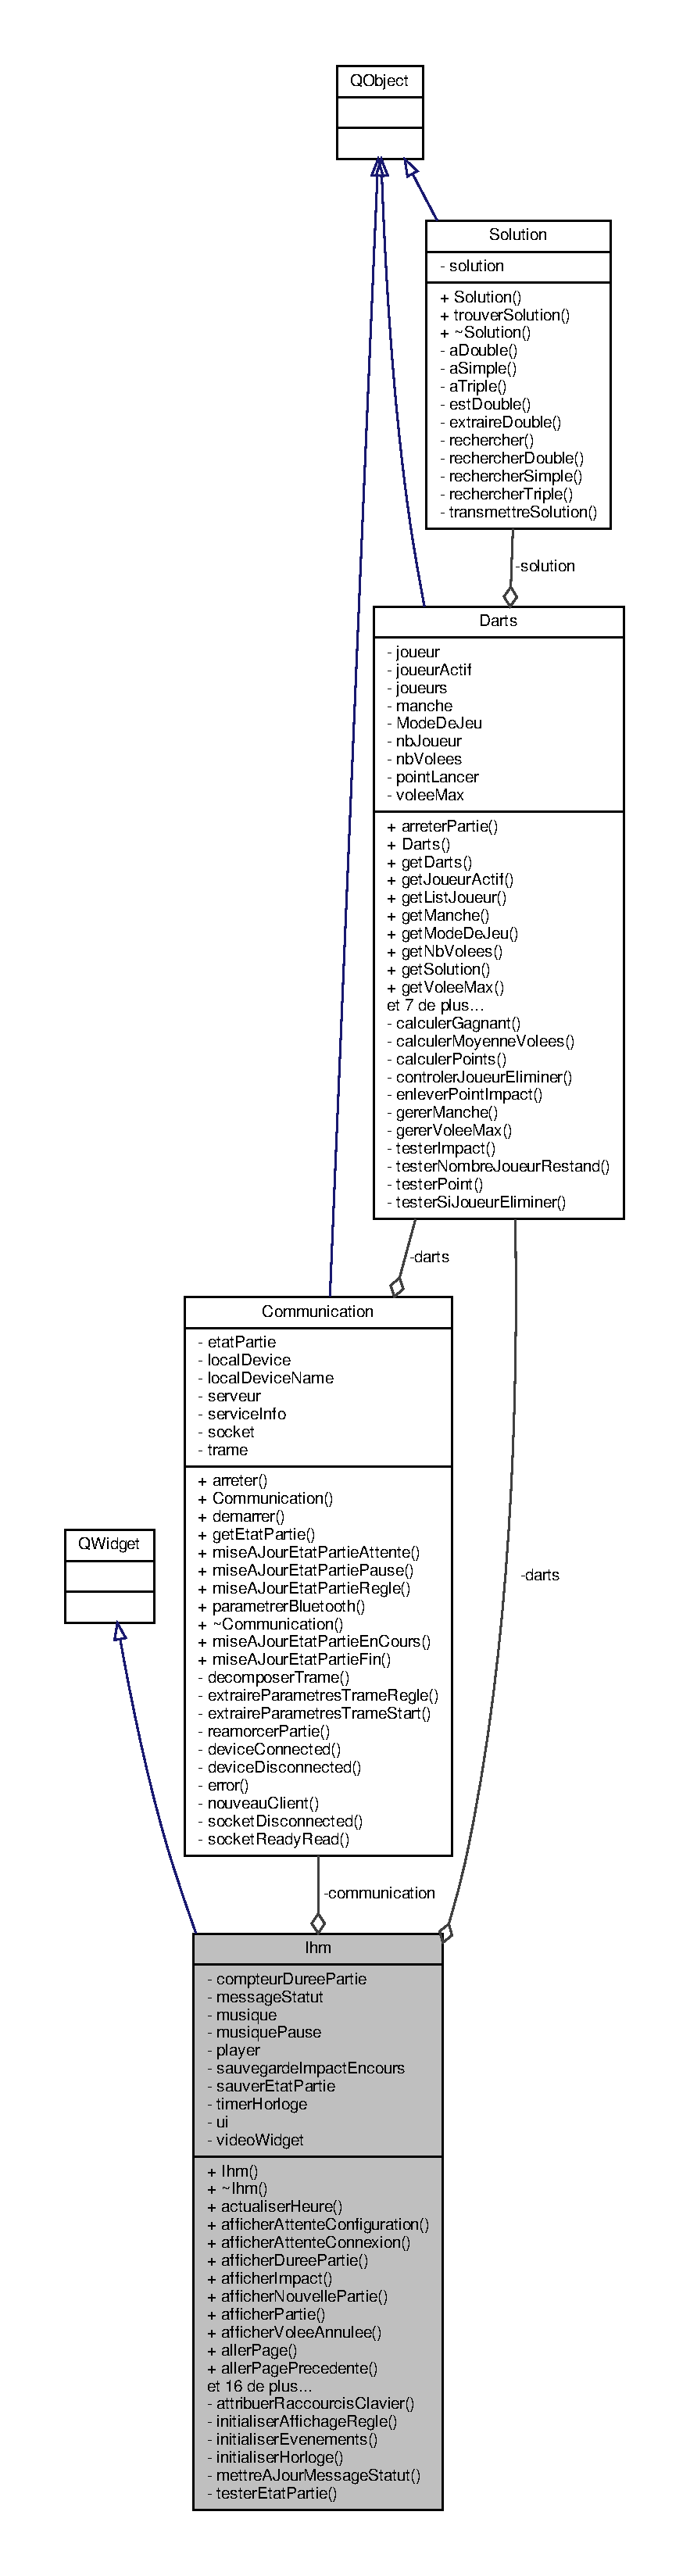
\includegraphics[height=550pt]{class_ihm__coll__graph}
\end{center}
\end{figure}
\subsubsection*{Connecteurs publics}
\begin{DoxyCompactItemize}
\item 
void \hyperlink{class_ihm_ad8b3b13e638ebbfbe8159d00d99ff88f}{actualiser\+Heure} ()
\begin{DoxyCompactList}\small\item\em Méthode qui met a jour l\textquotesingle{}heure sur l\textquotesingle{}application. \end{DoxyCompactList}\item 
void \hyperlink{class_ihm_a3d1f9b366774b538acfcf66195c3c81a}{afficher\+Attente\+Configuration} ()
\begin{DoxyCompactList}\small\item\em Méthode qui permet de mettre a jour le message de status \char`\"{}nouvelle appareil connecté\char`\"{}. \end{DoxyCompactList}\item 
void \hyperlink{class_ihm_a46f511e7be2c138a8fe2dec17d6bb2bf}{afficher\+Attente\+Connexion} ()
\begin{DoxyCompactList}\small\item\em Méthode qui permet de mettre a jour le message de status \char`\"{}appareil deconnecté\char`\"{}. \end{DoxyCompactList}\item 
void \hyperlink{class_ihm_a808bd550b877499a38419a492595822e}{afficher\+Duree\+Partie} ()
\begin{DoxyCompactList}\small\item\em Affiche la durée d\textquotesingle{}une Seance(slot) \end{DoxyCompactList}\item 
void \hyperlink{class_ihm_a591e686d87b027ac16e91b3b9867a58a}{afficher\+Impact} (int type\+Point, int point)
\begin{DoxyCompactList}\small\item\em Méthode qui affiche la cible correspondante à l\textquotesingle{}impact (si fichier Image Impact et disponible) et les points de cette Impact. \end{DoxyCompactList}\item 
void \hyperlink{class_ihm_a90c6b5c75d3903f50ea7c00b8093c686}{afficher\+Nouvelle\+Partie} ()
\begin{DoxyCompactList}\small\item\em Méthode qui met à jour l\textquotesingle{}affichage pour lancer une nouvelle partie. \end{DoxyCompactList}\item 
void \hyperlink{class_ihm_a3b26fb5299eba99925d005ea39eef9da}{afficher\+Partie} ()
\begin{DoxyCompactList}\small\item\em Méthode qui met a jour le mode de jeu et la page actif. \end{DoxyCompactList}\item 
void \hyperlink{class_ihm_a066192d0a1b9c241a67032b0c3c96be6}{afficher\+Volee\+Annulee} ()
\begin{DoxyCompactList}\small\item\em Méthode qui affiche le message de statut \char`\"{}volée annulée\char`\"{}. \end{DoxyCompactList}\item 
void \hyperlink{class_ihm_a52bf0bd258d00a16d3e1037a9288948b}{aller\+Page} (\hyperlink{class_ihm_a472c7a7bec7e6e0230842f78ace4833e}{Ihm\+::\+Page} page)
\begin{DoxyCompactList}\small\item\em Méthode qui permet de changer de Q\+Stacked\+Widget avec la Précédente. \end{DoxyCompactList}\item 
void \hyperlink{class_ihm_ac63f9c49fbde4482bb28e7f7e5882b25}{aller\+Page\+Precedente} ()
\begin{DoxyCompactList}\small\item\em Méthode qui permet de changer de Q\+Stacked\+Widget avec la Précédente. \end{DoxyCompactList}\item 
void \hyperlink{class_ihm_a3c53027b16e9ed5f669b9865b2057e6a}{aller\+Page\+Suivante} ()
\begin{DoxyCompactList}\small\item\em Méthode qui permet de changer de Q\+Stacked\+Widget avec la suivante. \end{DoxyCompactList}\item 
void \hyperlink{class_ihm_a28b5dd043c4d752bb944110d8d8457aa}{error} (Q\+Media\+Player\+::\+Error error)
\begin{DoxyCompactList}\small\item\em Méthode appelée quand il y a une erreur de vidéo. \end{DoxyCompactList}\item 
void \hyperlink{class_ihm_a703fa568eb3a2fb7f912decad222817e}{fermer\+Application} ()
\begin{DoxyCompactList}\small\item\em Méthode qui permet de quitter l\textquotesingle{}application. \end{DoxyCompactList}\item 
void \hyperlink{class_ihm_a0c7ee6ee6313db87c7cc34dbd57dd57d}{finir\+Partie} (Q\+String gagnant, int volee\+Max\+Joueur)
\begin{DoxyCompactList}\small\item\em Méthode qui met à jour l\textquotesingle{}affichage quand la partie est fini. \end{DoxyCompactList}\item 
void \hyperlink{class_ihm_a55f2d106f7af9ed2e84f78822e23bb97}{jouer\+Son} (Q\+String son)
\begin{DoxyCompactList}\small\item\em Méthode qui permet de jouer un son. \end{DoxyCompactList}\item 
void \hyperlink{class_ihm_a5186bc159a8bf1fa359da4f4ccd78f5a}{lancer\+Regle} (Q\+String regle)
\begin{DoxyCompactList}\small\item\em Méthode qui lance la vidéo explicative des regles suivant le type de jeu. \end{DoxyCompactList}\item 
void \hyperlink{class_ihm_a3c504c417aa2d3efd82ac5feded16895}{mettre\+A\+Jour\+Cible} ()
\begin{DoxyCompactList}\small\item\em Méthode qui reinitialise l\textquotesingle{}affichage de la cible. \end{DoxyCompactList}\item 
void \hyperlink{class_ihm_aaeeb08a39f940e58da194768763dc00b}{mettre\+A\+Jour\+Joueur} ()
\begin{DoxyCompactList}\small\item\em Méthode qui initialise l\textquotesingle{}affichage du mode et des joueurs de la partie. \end{DoxyCompactList}\item 
void \hyperlink{class_ihm_a3b41d92919b87966f903b22863dc6acb}{mettre\+A\+Jour\+Manche} ()
\begin{DoxyCompactList}\small\item\em Méthode qui met à jour le numero de la manche. \end{DoxyCompactList}\item 
void \hyperlink{class_ihm_a7837ec36fbac1ca96d049ad27263b951}{mettre\+A\+Jour\+Message\+Statut} (Q\+String)
\begin{DoxyCompactList}\small\item\em Méthode qui met à jour le message de statut. \end{DoxyCompactList}\item 
void \hyperlink{class_ihm_abafc4398a910be8ab95a75fbdf176426}{mettre\+A\+Jour\+Moyenne\+Volee} ()
\begin{DoxyCompactList}\small\item\em Méthode qui initialise l\textquotesingle{}affichage du mode et des joueurs de la partie. \end{DoxyCompactList}\item 
void \hyperlink{class_ihm_a238255f517506367fe8913b2dad50c65}{mettre\+A\+Jour\+Score} ()
\begin{DoxyCompactList}\small\item\em Méthode qui met à jour le score dans L\textquotesingle{}ihm. \end{DoxyCompactList}\item 
void \hyperlink{class_ihm_a27b24d133887431399b4696a4eae02e6}{mettre\+A\+Joursolution} (Q\+String solution)
\begin{DoxyCompactList}\small\item\em Affiche les solutions possibles pour finir la parties. \end{DoxyCompactList}\item 
void \hyperlink{class_ihm_ab8456da276715f99ba373b71313592de}{mettre\+Pause\+Partie} ()
\begin{DoxyCompactList}\small\item\em Mets en pause le chronométrage de la partiee. \end{DoxyCompactList}\item 
void \hyperlink{class_ihm_a3480957ba23548b30dddc717f6cfa577}{relancerpartie} ()
\begin{DoxyCompactList}\small\item\em relancer le chronométrage de la partie \end{DoxyCompactList}\item 
void \hyperlink{class_ihm_a3c815827527ca8f9c586e001e8e95721}{state\+Changed} (Q\+Media\+Player\+::\+State state)
\begin{DoxyCompactList}\small\item\em Méthode appelée quand l\textquotesingle{}état de la vidéo change. \end{DoxyCompactList}\end{DoxyCompactItemize}
\subsubsection*{Fonctions membres publiques}
\begin{DoxyCompactItemize}
\item 
\hyperlink{class_ihm_a50a7a15775452923868348bdbe4fa51e}{Ihm} (\hyperlink{class_q_widget}{Q\+Widget} $\ast$parent=nullptr)
\begin{DoxyCompactList}\small\item\em Constructeur de la classe \hyperlink{class_ihm}{Ihm}. \end{DoxyCompactList}\item 
\hyperlink{class_ihm_add292ea9005bacd1de44dd1ed9ede5b9}{$\sim$\+Ihm} ()
\begin{DoxyCompactList}\small\item\em Destructeur de la classe \hyperlink{class_ihm}{Ihm}. \end{DoxyCompactList}\end{DoxyCompactItemize}
\subsubsection*{Types privés}
\begin{DoxyCompactItemize}
\item 
enum \hyperlink{class_ihm_a472c7a7bec7e6e0230842f78ace4833e}{Page} \{ \newline
\hyperlink{class_ihm_a472c7a7bec7e6e0230842f78ace4833ea6c6994098bc403f5ec5f712c347ce622}{Page\+Attente} = 0, 
\hyperlink{class_ihm_a472c7a7bec7e6e0230842f78ace4833eaeb2ec486b2e880de96d76609d12c36af}{Page\+Regle}, 
\hyperlink{class_ihm_a472c7a7bec7e6e0230842f78ace4833eadc27359267c694f4d9c3afc23fe8b82f}{Page\+Jeu}, 
\hyperlink{class_ihm_a472c7a7bec7e6e0230842f78ace4833eaacc428ff827bccfb5e8bdb4634457f10}{Page\+Statistique}, 
\newline
\hyperlink{class_ihm_a472c7a7bec7e6e0230842f78ace4833ea9eb2cac6f79bce4cfd72383724004949}{Nb\+Pages}
 \}\begin{DoxyCompactList}\small\item\em Définit les différentes pages de l\textquotesingle{}I\+HM. \end{DoxyCompactList}
\end{DoxyCompactItemize}
\subsubsection*{Fonctions membres privées}
\begin{DoxyCompactItemize}
\item 
void \hyperlink{class_ihm_a2b7dbb2d087d4ca15cee9707a1796b62}{attribuer\+Raccourcis\+Clavier} ()
\begin{DoxyCompactList}\small\item\em Méthode qui initialise les raccourcis clavier. \end{DoxyCompactList}\item 
void \hyperlink{class_ihm_a97b1938c38eef2427b5cf2326feeef3d}{initialiser\+Affichage\+Regle} ()
\begin{DoxyCompactList}\small\item\em Méthode qui initialise l\textquotesingle{}affichage vidéo des règles. \end{DoxyCompactList}\item 
void \hyperlink{class_ihm_a9df8990148a898f728304a4e789be2a6}{initialiser\+Evenements} ()
\begin{DoxyCompactList}\small\item\em Méthode qui initialise les connexion signals/slots de Qt. \end{DoxyCompactList}\item 
void \hyperlink{class_ihm_aa5a3e97de39e919ea8807d30167da510}{initialiser\+Horloge} ()
\begin{DoxyCompactList}\small\item\em initialise l\textquotesingle{}horloge pour un affichage périodique \end{DoxyCompactList}\item 
void \hyperlink{class_ihm_ab80e655c95fca8e1113343bdbd3d3586}{mettre\+A\+Jour\+Message\+Statut} (int type\+Point, int point)
\begin{DoxyCompactList}\small\item\em Méthode qui met à jour le message de statut de la volée en cours. \end{DoxyCompactList}\item 
void \hyperlink{class_ihm_a8dbd08db43f7c80ca7266cc6b162f571}{tester\+Etat\+Partie} ()
\begin{DoxyCompactList}\small\item\em Méthode appelée pour remettre l\textquotesingle{}état dans lequel était la partie avant l\textquotesingle{}affichage des règles. \end{DoxyCompactList}\end{DoxyCompactItemize}
\subsubsection*{Attributs privés}
\begin{DoxyCompactItemize}
\item 
\hyperlink{class_communication}{Communication} $\ast$ \hyperlink{class_ihm_a2f3d4781795781a840786cd8c2233899}{communication}
\begin{DoxyCompactList}\small\item\em objet communication \end{DoxyCompactList}\item 
int \hyperlink{class_ihm_a61e4a83f8ca0f177971af808e51be5bb}{compteur\+Duree\+Partie}
\begin{DoxyCompactList}\small\item\em compteur de secondes pour la durée d\textquotesingle{}une séance \end{DoxyCompactList}\item 
\hyperlink{class_darts}{Darts} $\ast$ \hyperlink{class_ihm_a2a0f54d33f4d6b2531ec2190c4a2356e}{darts}
\begin{DoxyCompactList}\small\item\em objet darts \end{DoxyCompactList}\item 
Q\+String \hyperlink{class_ihm_a31a25b36e5560142cb156b8b1a25965f}{message\+Statut}
\begin{DoxyCompactList}\small\item\em contient le message de statut qui est affiché \end{DoxyCompactList}\item 
Q\+Sound \hyperlink{class_ihm_a6e2a173ec36ee846d6210117b4b85fa8}{musique}
\begin{DoxyCompactList}\small\item\em objet musique \end{DoxyCompactList}\item 
Q\+Sound \hyperlink{class_ihm_a11e7ae529b6adb7ac98f1aa512172ff2}{musique\+Pause}
\begin{DoxyCompactList}\small\item\em objet musique\+Pause \end{DoxyCompactList}\item 
Q\+Media\+Player $\ast$ \hyperlink{class_ihm_a633230fb15d587e647ad9d2d6142ebc3}{player}
\begin{DoxyCompactList}\small\item\em objet player \end{DoxyCompactList}\item 
Q\+Pixmap \hyperlink{class_ihm_a659c67bf5d1ba3104fb10f23d8b91b37}{sauvegarde\+Impact\+Encours}
\begin{DoxyCompactList}\small\item\em sauvegarde le Q\+Pixmap de l\textquotesingle{}état de la cible \end{DoxyCompactList}\item 
int \hyperlink{class_ihm_a1a9d23dd4defa0b88d1e4a56ce807e45}{sauver\+Etat\+Partie}
\begin{DoxyCompactList}\small\item\em Contient l\textquotesingle{}état de la partie avant l\textquotesingle{}affichage des règles. \end{DoxyCompactList}\item 
Q\+Timer $\ast$ \hyperlink{class_ihm_a21ea35b212966fa2805241ea6237d351}{timer\+Horloge}
\begin{DoxyCompactList}\small\item\em objet timer\+Horloge \end{DoxyCompactList}\item 
Ui\+::\+Ihm $\ast$ \hyperlink{class_ihm_a0ac5f47856566ceeeca1720109bf70ea}{ui}
\begin{DoxyCompactList}\small\item\em object de notre \hyperlink{class_ihm}{Ihm} \end{DoxyCompactList}\item 
Q\+Video\+Widget $\ast$ \hyperlink{class_ihm_a011827612654af9b19bc8c42045e3c06}{video\+Widget}
\begin{DoxyCompactList}\small\item\em objet video\+Widget \end{DoxyCompactList}\end{DoxyCompactItemize}


\subsubsection{Description détaillée}
Déclaration de la classe \hyperlink{class_ihm}{Ihm} (Module Ecran-\/\+D\+A\+R\+TS) 

Cette classe s\textquotesingle{}occupe de l\textquotesingle{}affichage sur l\textquotesingle{}écran 

Définition à la ligne \hyperlink{ihm_8h_source_l00043}{43} du fichier \hyperlink{ihm_8h_source}{ihm.\+h}.



\subsubsection{Documentation des énumérations membres}
\mbox{\Hypertarget{class_ihm_a472c7a7bec7e6e0230842f78ace4833e}\label{class_ihm_a472c7a7bec7e6e0230842f78ace4833e}} 
\index{Ihm@{Ihm}!Page@{Page}}
\index{Page@{Page}!Ihm@{Ihm}}
\paragraph{\texorpdfstring{Page}{Page}}
{\footnotesize\ttfamily enum \hyperlink{class_ihm_a472c7a7bec7e6e0230842f78ace4833e}{Ihm\+::\+Page}\hspace{0.3cm}{\ttfamily [private]}}



Définit les différentes pages de l\textquotesingle{}I\+HM. 

\begin{DoxyEnumFields}{Valeurs énumérées}
\raisebox{\heightof{T}}[0pt][0pt]{\index{Page\+Attente@{Page\+Attente}!Ihm@{Ihm}}\index{Ihm@{Ihm}!Page\+Attente@{Page\+Attente}}}\mbox{\Hypertarget{class_ihm_a472c7a7bec7e6e0230842f78ace4833ea6c6994098bc403f5ec5f712c347ce622}\label{class_ihm_a472c7a7bec7e6e0230842f78ace4833ea6c6994098bc403f5ec5f712c347ce622}} 
Page\+Attente&\\
\hline

\raisebox{\heightof{T}}[0pt][0pt]{\index{Page\+Regle@{Page\+Regle}!Ihm@{Ihm}}\index{Ihm@{Ihm}!Page\+Regle@{Page\+Regle}}}\mbox{\Hypertarget{class_ihm_a472c7a7bec7e6e0230842f78ace4833eaeb2ec486b2e880de96d76609d12c36af}\label{class_ihm_a472c7a7bec7e6e0230842f78ace4833eaeb2ec486b2e880de96d76609d12c36af}} 
Page\+Regle&\\
\hline

\raisebox{\heightof{T}}[0pt][0pt]{\index{Page\+Jeu@{Page\+Jeu}!Ihm@{Ihm}}\index{Ihm@{Ihm}!Page\+Jeu@{Page\+Jeu}}}\mbox{\Hypertarget{class_ihm_a472c7a7bec7e6e0230842f78ace4833eadc27359267c694f4d9c3afc23fe8b82f}\label{class_ihm_a472c7a7bec7e6e0230842f78ace4833eadc27359267c694f4d9c3afc23fe8b82f}} 
Page\+Jeu&\\
\hline

\raisebox{\heightof{T}}[0pt][0pt]{\index{Page\+Statistique@{Page\+Statistique}!Ihm@{Ihm}}\index{Ihm@{Ihm}!Page\+Statistique@{Page\+Statistique}}}\mbox{\Hypertarget{class_ihm_a472c7a7bec7e6e0230842f78ace4833eaacc428ff827bccfb5e8bdb4634457f10}\label{class_ihm_a472c7a7bec7e6e0230842f78ace4833eaacc428ff827bccfb5e8bdb4634457f10}} 
Page\+Statistique&\\
\hline

\raisebox{\heightof{T}}[0pt][0pt]{\index{Nb\+Pages@{Nb\+Pages}!Ihm@{Ihm}}\index{Ihm@{Ihm}!Nb\+Pages@{Nb\+Pages}}}\mbox{\Hypertarget{class_ihm_a472c7a7bec7e6e0230842f78ace4833ea9eb2cac6f79bce4cfd72383724004949}\label{class_ihm_a472c7a7bec7e6e0230842f78ace4833ea9eb2cac6f79bce4cfd72383724004949}} 
Nb\+Pages&\\
\hline

\end{DoxyEnumFields}


Définition à la ligne \hyperlink{ihm_8h_source_l00072}{72} du fichier \hyperlink{ihm_8h_source}{ihm.\+h}.


\begin{DoxyCode}
00073     \{
00074         \hyperlink{class_ihm_a472c7a7bec7e6e0230842f78ace4833ea6c6994098bc403f5ec5f712c347ce622}{PageAttente} = 0,
00075         \hyperlink{class_ihm_a472c7a7bec7e6e0230842f78ace4833eaeb2ec486b2e880de96d76609d12c36af}{PageRegle},
00076         \hyperlink{class_ihm_a472c7a7bec7e6e0230842f78ace4833eadc27359267c694f4d9c3afc23fe8b82f}{PageJeu},
00077         \hyperlink{class_ihm_a472c7a7bec7e6e0230842f78ace4833eaacc428ff827bccfb5e8bdb4634457f10}{PageStatistique},
00078         \hyperlink{class_ihm_a472c7a7bec7e6e0230842f78ace4833ea9eb2cac6f79bce4cfd72383724004949}{NbPages}
00079     \};
\end{DoxyCode}


\subsubsection{Documentation des constructeurs et destructeur}
\mbox{\Hypertarget{class_ihm_a50a7a15775452923868348bdbe4fa51e}\label{class_ihm_a50a7a15775452923868348bdbe4fa51e}} 
\index{Ihm@{Ihm}!Ihm@{Ihm}}
\index{Ihm@{Ihm}!Ihm@{Ihm}}
\paragraph{\texorpdfstring{Ihm()}{Ihm()}}
{\footnotesize\ttfamily Ihm\+::\+Ihm (\begin{DoxyParamCaption}\item[{\hyperlink{class_q_widget}{Q\+Widget} $\ast$}]{parent = {\ttfamily nullptr} }\end{DoxyParamCaption})\hspace{0.3cm}{\ttfamily [explicit]}}



Constructeur de la classe \hyperlink{class_ihm}{Ihm}. 


\begin{DoxyParams}{Paramètres}
{\em parent} & \\
\hline
\end{DoxyParams}


Définition à la ligne \hyperlink{ihm_8cpp_source_l00026}{26} du fichier \hyperlink{ihm_8cpp_source}{ihm.\+cpp}.



Références \hyperlink{ihm_8cpp_source_l00383}{afficher\+Nouvelle\+Partie()}, \hyperlink{ihm_8cpp_source_l00103}{attribuer\+Raccourcis\+Clavier()}, \hyperlink{ihm_8h_source_l00054}{communication}, \hyperlink{ihm_8h_source_l00055}{darts}, \hyperlink{communication_8cpp_source_l00101}{Communication\+::demarrer()}, \hyperlink{ihm_8cpp_source_l00605}{initialiser\+Affichage\+Regle()}, \hyperlink{ihm_8cpp_source_l00075}{initialiser\+Evenements()}, \hyperlink{ihm_8cpp_source_l00553}{initialiser\+Horloge()}, et \hyperlink{ihm_8h_source_l00052}{ui}.


\begin{DoxyCode}
00026                         :
00027     \hyperlink{class_q_widget}{QWidget}(parent),
00028     \hyperlink{class_ihm_a0ac5f47856566ceeeca1720109bf70ea}{ui}(\textcolor{keyword}{new} Ui::Ihm),
00029     \hyperlink{class_ihm_a6e2a173ec36ee846d6210117b4b85fa8}{musique}(qApp->applicationDirPath() + \hyperlink{ihm_8h_aaf7f17312e64cf24f4c93fc657e5594f}{CHEMIN\_FICHIER\_MUSIQUE} + \textcolor{stringliteral}{"music.wav"},\textcolor{keyword}{
      this}),
00030     \hyperlink{class_ihm_a11e7ae529b6adb7ac98f1aa512172ff2}{musiquePause}(qApp->applicationDirPath() + \hyperlink{ihm_8h_aaf7f17312e64cf24f4c93fc657e5594f}{CHEMIN\_FICHIER\_MUSIQUE} + \textcolor{stringliteral}{"
      pause.wav"},\textcolor{keyword}{this}),
00031     \hyperlink{class_ihm_a61e4a83f8ca0f177971af808e51be5bb}{compteurDureePartie}(0),
00032     \hyperlink{class_ihm_a31a25b36e5560142cb156b8b1a25965f}{messageStatut}(\textcolor{stringliteral}{"Volée ➤"})
00033 \{
00034     \hyperlink{class_ihm_a0ac5f47856566ceeeca1720109bf70ea}{ui}->setupUi(\textcolor{keyword}{this});
00035     qDebug() << Q\_FUNC\_INFO;
00036 
00037     \hyperlink{class_ihm_a2a0f54d33f4d6b2531ec2190c4a2356e}{darts} = \textcolor{keyword}{new} \hyperlink{class_darts}{Darts}(\textcolor{keyword}{this});
00038     \hyperlink{class_ihm_a2f3d4781795781a840786cd8c2233899}{communication} = \textcolor{keyword}{new} \hyperlink{class_communication}{Communication}(\hyperlink{class_ihm_a2a0f54d33f4d6b2531ec2190c4a2356e}{darts}, \textcolor{keyword}{this});
00039 
00040     \textcolor{comment}{// Initialiser l'horloge}
00041     \hyperlink{class_ihm_aa5a3e97de39e919ea8807d30167da510}{initialiserHorloge}();
00042 
00043     \textcolor{comment}{// Raccourcis Quitter/ChangerPage (mode debug)}
00044     \hyperlink{class_ihm_a2b7dbb2d087d4ca15cee9707a1796b62}{attribuerRaccourcisClavier}();
00045 
00046     \textcolor{comment}{// Démarrer la communication bluetooth}
00047     \hyperlink{class_ihm_a2f3d4781795781a840786cd8c2233899}{communication}->\hyperlink{class_communication_af29ea9a1c2ce29436f2331c322f6ebbf}{demarrer}();
00048 
00049     \textcolor{comment}{// Initialiser les connexions signal/slot}
00050     \hyperlink{class_ihm_a9df8990148a898f728304a4e789be2a6}{initialiserEvenements}();
00051 
00052     \textcolor{comment}{//configuration affichage des regles}
00053     \hyperlink{class_ihm_a97b1938c38eef2427b5cf2326feeef3d}{initialiserAffichageRegle}();
00054 
00055     \textcolor{comment}{//Afficher la page d'attente}
00056     \hyperlink{class_ihm_a90c6b5c75d3903f50ea7c00b8093c686}{afficherNouvellePartie}();
00057 \}
\end{DoxyCode}
\mbox{\Hypertarget{class_ihm_add292ea9005bacd1de44dd1ed9ede5b9}\label{class_ihm_add292ea9005bacd1de44dd1ed9ede5b9}} 
\index{Ihm@{Ihm}!````~Ihm@{$\sim$\+Ihm}}
\index{````~Ihm@{$\sim$\+Ihm}!Ihm@{Ihm}}
\paragraph{\texorpdfstring{$\sim$\+Ihm()}{~Ihm()}}
{\footnotesize\ttfamily Ihm\+::$\sim$\+Ihm (\begin{DoxyParamCaption}{ }\end{DoxyParamCaption})}



Destructeur de la classe \hyperlink{class_ihm}{Ihm}. 



Définition à la ligne \hyperlink{ihm_8cpp_source_l00064}{64} du fichier \hyperlink{ihm_8cpp_source}{ihm.\+cpp}.



Références \hyperlink{ihm_8h_source_l00052}{ui}.


\begin{DoxyCode}
00065 \{
00066     \textcolor{keyword}{delete} \hyperlink{class_ihm_a0ac5f47856566ceeeca1720109bf70ea}{ui};
00067     qDebug() << Q\_FUNC\_INFO;
00068 \}
\end{DoxyCode}


\subsubsection{Documentation des fonctions membres}
\mbox{\Hypertarget{class_ihm_ad8b3b13e638ebbfbe8159d00d99ff88f}\label{class_ihm_ad8b3b13e638ebbfbe8159d00d99ff88f}} 
\index{Ihm@{Ihm}!actualiser\+Heure@{actualiser\+Heure}}
\index{actualiser\+Heure@{actualiser\+Heure}!Ihm@{Ihm}}
\paragraph{\texorpdfstring{actualiser\+Heure}{actualiserHeure}}
{\footnotesize\ttfamily void Ihm\+::actualiser\+Heure (\begin{DoxyParamCaption}{ }\end{DoxyParamCaption})\hspace{0.3cm}{\ttfamily [slot]}}



Méthode qui met a jour l\textquotesingle{}heure sur l\textquotesingle{}application. 



Définition à la ligne \hyperlink{ihm_8cpp_source_l00127}{127} du fichier \hyperlink{ihm_8cpp_source}{ihm.\+cpp}.



Références \hyperlink{ihm_8h_source_l00052}{ui}.



Référencé par \hyperlink{ihm_8cpp_source_l00553}{initialiser\+Horloge()}.


\begin{DoxyCode}
00128 \{
00129     QString affichageHeure;
00130     QTime heure = QTime::currentTime();
00131     affichageHeure = \textcolor{stringliteral}{"<font color=\(\backslash\)"#6D2B6B\(\backslash\)">"} + heure.toString(\textcolor{stringliteral}{"hh : mm "}) + \textcolor{stringliteral}{"</font>"};
00132     \hyperlink{class_ihm_a0ac5f47856566ceeeca1720109bf70ea}{ui}->labelHeureAttente->setText(affichageHeure);
00133     \hyperlink{class_ihm_a0ac5f47856566ceeeca1720109bf70ea}{ui}->labelHeureStatistique->setText(affichageHeure);
00134 \}
\end{DoxyCode}
\mbox{\Hypertarget{class_ihm_a3d1f9b366774b538acfcf66195c3c81a}\label{class_ihm_a3d1f9b366774b538acfcf66195c3c81a}} 
\index{Ihm@{Ihm}!afficher\+Attente\+Configuration@{afficher\+Attente\+Configuration}}
\index{afficher\+Attente\+Configuration@{afficher\+Attente\+Configuration}!Ihm@{Ihm}}
\paragraph{\texorpdfstring{afficher\+Attente\+Configuration}{afficherAttenteConfiguration}}
{\footnotesize\ttfamily void Ihm\+::afficher\+Attente\+Configuration (\begin{DoxyParamCaption}{ }\end{DoxyParamCaption})\hspace{0.3cm}{\ttfamily [slot]}}



Méthode qui permet de mettre a jour le message de status \char`\"{}nouvelle appareil connecté\char`\"{}. 



Définition à la ligne \hyperlink{ihm_8cpp_source_l00463}{463} du fichier \hyperlink{ihm_8cpp_source}{ihm.\+cpp}.



Références \hyperlink{ihm_8h_source_l00052}{ui}.



Référencé par \hyperlink{ihm_8cpp_source_l00075}{initialiser\+Evenements()}.


\begin{DoxyCode}
00464 \{
00465     \hyperlink{class_ihm_a0ac5f47856566ceeeca1720109bf70ea}{ui}->labelStatutAttente->setText(\textcolor{stringliteral}{"Attente configuration de la partie"});
00466 \}
\end{DoxyCode}
\mbox{\Hypertarget{class_ihm_a46f511e7be2c138a8fe2dec17d6bb2bf}\label{class_ihm_a46f511e7be2c138a8fe2dec17d6bb2bf}} 
\index{Ihm@{Ihm}!afficher\+Attente\+Connexion@{afficher\+Attente\+Connexion}}
\index{afficher\+Attente\+Connexion@{afficher\+Attente\+Connexion}!Ihm@{Ihm}}
\paragraph{\texorpdfstring{afficher\+Attente\+Connexion}{afficherAttenteConnexion}}
{\footnotesize\ttfamily void Ihm\+::afficher\+Attente\+Connexion (\begin{DoxyParamCaption}{ }\end{DoxyParamCaption})\hspace{0.3cm}{\ttfamily [slot]}}



Méthode qui permet de mettre a jour le message de status \char`\"{}appareil deconnecté\char`\"{}. 



Définition à la ligne \hyperlink{ihm_8cpp_source_l00473}{473} du fichier \hyperlink{ihm_8cpp_source}{ihm.\+cpp}.



Références \hyperlink{ihm_8h_source_l00052}{ui}.



Référencé par \hyperlink{ihm_8cpp_source_l00075}{initialiser\+Evenements()}.


\begin{DoxyCode}
00474 \{
00475     \hyperlink{class_ihm_a0ac5f47856566ceeeca1720109bf70ea}{ui}->labelStatutAttente->setText(\textcolor{stringliteral}{"En attente de connexion"});
00476 \}
\end{DoxyCode}
\mbox{\Hypertarget{class_ihm_a808bd550b877499a38419a492595822e}\label{class_ihm_a808bd550b877499a38419a492595822e}} 
\index{Ihm@{Ihm}!afficher\+Duree\+Partie@{afficher\+Duree\+Partie}}
\index{afficher\+Duree\+Partie@{afficher\+Duree\+Partie}!Ihm@{Ihm}}
\paragraph{\texorpdfstring{afficher\+Duree\+Partie}{afficherDureePartie}}
{\footnotesize\ttfamily void Ihm\+::afficher\+Duree\+Partie (\begin{DoxyParamCaption}{ }\end{DoxyParamCaption})\hspace{0.3cm}{\ttfamily [slot]}}



Affiche la durée d\textquotesingle{}une Seance(slot) 



Définition à la ligne \hyperlink{ihm_8cpp_source_l00484}{484} du fichier \hyperlink{ihm_8cpp_source}{ihm.\+cpp}.



Références \hyperlink{ihm_8h_source_l00058}{compteur\+Duree\+Partie}, et \hyperlink{ihm_8h_source_l00052}{ui}.



Référencé par \hyperlink{ihm_8cpp_source_l00333}{afficher\+Partie()}, \hyperlink{ihm_8cpp_source_l00365}{finir\+Partie()}, \hyperlink{ihm_8cpp_source_l00519}{mettre\+Pause\+Partie()}, et \hyperlink{ihm_8cpp_source_l00539}{relancerpartie()}.


\begin{DoxyCode}
00485 \{
00486     QTime duree(0, 0);
00487     \hyperlink{class_ihm_a61e4a83f8ca0f177971af808e51be5bb}{compteurDureePartie}++;
00488     QTime dureeSeance = duree.addSecs(\hyperlink{class_ihm_a61e4a83f8ca0f177971af808e51be5bb}{compteurDureePartie});
00489     \textcolor{keywordflow}{if}(\hyperlink{class_ihm_a61e4a83f8ca0f177971af808e51be5bb}{compteurDureePartie} >= 3600)
00490     \{
00491         \hyperlink{class_ihm_a0ac5f47856566ceeeca1720109bf70ea}{ui}->ecranPartie->setStyleSheet(\textcolor{stringliteral}{"
      QWidget#ecranPartie\{background-image:url(:/ressources/backgroundHeure.jpg);\}"});
00492         \hyperlink{class_ihm_a0ac5f47856566ceeeca1720109bf70ea}{ui}->labelTempsPartie->setText(dureeSeance.toString(\textcolor{stringliteral}{"hh : mm : ss"}));
00493         \hyperlink{class_ihm_a0ac5f47856566ceeeca1720109bf70ea}{ui}->tempsPartie->setText(dureeSeance.toString(\textcolor{stringliteral}{"hh : mm : ss"}));
00494     \}
00495     \textcolor{keywordflow}{else}
00496     \{
00497         \hyperlink{class_ihm_a0ac5f47856566ceeeca1720109bf70ea}{ui}->labelTempsPartie->setText(dureeSeance.toString(\textcolor{stringliteral}{"mm : ss"}));
00498         \hyperlink{class_ihm_a0ac5f47856566ceeeca1720109bf70ea}{ui}->tempsPartie->setText(dureeSeance.toString(\textcolor{stringliteral}{"mm : ss"}));
00499     \}
00500 \}
\end{DoxyCode}
\mbox{\Hypertarget{class_ihm_a591e686d87b027ac16e91b3b9867a58a}\label{class_ihm_a591e686d87b027ac16e91b3b9867a58a}} 
\index{Ihm@{Ihm}!afficher\+Impact@{afficher\+Impact}}
\index{afficher\+Impact@{afficher\+Impact}!Ihm@{Ihm}}
\paragraph{\texorpdfstring{afficher\+Impact}{afficherImpact}}
{\footnotesize\ttfamily void Ihm\+::afficher\+Impact (\begin{DoxyParamCaption}\item[{int}]{type\+Point,  }\item[{int}]{point }\end{DoxyParamCaption})\hspace{0.3cm}{\ttfamily [slot]}}



Méthode qui affiche la cible correspondante à l\textquotesingle{}impact (si fichier Image Impact et disponible) et les points de cette Impact. 


\begin{DoxyParams}{Paramètres}
{\em type\+Point} & \\
\hline
{\em point} & \\
\hline
\end{DoxyParams}


Définition à la ligne \hyperlink{ihm_8cpp_source_l00191}{191} du fichier \hyperlink{ihm_8cpp_source}{ihm.\+cpp}.



Références \hyperlink{ihm_8cpp_source_l00218}{mettre\+A\+Jour\+Message\+Statut()}, et \hyperlink{ihm_8h_source_l00052}{ui}.



Référencé par \hyperlink{ihm_8cpp_source_l00075}{initialiser\+Evenements()}.


\begin{DoxyCode}
00192 \{
00193     \textcolor{keywordflow}{if}(QFileInfo(qApp->applicationDirPath() + \textcolor{stringliteral}{"/impact/IMPACT\_"} + QString::number(typePoint) + \textcolor{stringliteral}{"\_"} + 
      QString::number(point) + \textcolor{stringliteral}{".png"}).exists())       \textcolor{comment}{//test si l'image existe}
00194     \{
00195         QImage impact(qApp->applicationDirPath() + \textcolor{stringliteral}{"/impact/IMPACT\_"} + QString::number(typePoint) + \textcolor{stringliteral}{"\_"} + 
      QString::number(point) + \textcolor{stringliteral}{".png"});
00196 
00197         QPixmap cibleImpacte = \hyperlink{class_ihm_a0ac5f47856566ceeeca1720109bf70ea}{ui}->labelVisualisationimpact->pixmap()->copy(); \textcolor{comment}{// on récupère l'image
       précédente;}
00198 
00199         QPainter p(&cibleImpacte);
00200 
00201         p.drawImage(QPoint(0, 0), impact);
00202 
00203         p.end();
00204 
00205         \hyperlink{class_ihm_a0ac5f47856566ceeeca1720109bf70ea}{ui}->labelVisualisationimpact->setPixmap(cibleImpacte);
00206     \}
00207 
00208     \hyperlink{class_ihm_ab80e655c95fca8e1113343bdbd3d3586}{mettreAJourMessageStatut}(typePoint, point);
00209 \}
\end{DoxyCode}
\mbox{\Hypertarget{class_ihm_a90c6b5c75d3903f50ea7c00b8093c686}\label{class_ihm_a90c6b5c75d3903f50ea7c00b8093c686}} 
\index{Ihm@{Ihm}!afficher\+Nouvelle\+Partie@{afficher\+Nouvelle\+Partie}}
\index{afficher\+Nouvelle\+Partie@{afficher\+Nouvelle\+Partie}!Ihm@{Ihm}}
\paragraph{\texorpdfstring{afficher\+Nouvelle\+Partie}{afficherNouvellePartie}}
{\footnotesize\ttfamily void Ihm\+::afficher\+Nouvelle\+Partie (\begin{DoxyParamCaption}{ }\end{DoxyParamCaption})\hspace{0.3cm}{\ttfamily [slot]}}



Méthode qui met à jour l\textquotesingle{}affichage pour lancer une nouvelle partie. 



Définition à la ligne \hyperlink{ihm_8cpp_source_l00383}{383} du fichier \hyperlink{ihm_8cpp_source}{ihm.\+cpp}.



Références \hyperlink{ihm_8cpp_source_l00429}{aller\+Page()}, \hyperlink{ihm_8cpp_source_l00565}{mettre\+A\+Jour\+Cible()}, \hyperlink{ihm_8h_source_l00056}{musique}, \hyperlink{ihm_8h_source_l00057}{musique\+Pause}, \hyperlink{ihm_8h_source_l00074}{Page\+Attente}, \hyperlink{ihm_8h_source_l00064}{player}, et \hyperlink{ihm_8h_source_l00052}{ui}.



Référencé par \hyperlink{ihm_8cpp_source_l00026}{Ihm()}, et \hyperlink{ihm_8cpp_source_l00075}{initialiser\+Evenements()}.


\begin{DoxyCode}
00384 \{
00385      \hyperlink{class_ihm_a633230fb15d587e647ad9d2d6142ebc3}{player}->stop();
00386      \hyperlink{class_ihm_a52bf0bd258d00a16d3e1037a9288948b}{allerPage}(\hyperlink{class_ihm_a472c7a7bec7e6e0230842f78ace4833ea6c6994098bc403f5ec5f712c347ce622}{Ihm::PageAttente});
00387      \hyperlink{class_ihm_a0ac5f47856566ceeeca1720109bf70ea}{ui}->manche->setText(\textcolor{stringliteral}{"1"});
00388      \hyperlink{class_ihm_a0ac5f47856566ceeeca1720109bf70ea}{ui}->nomJoueur->setText(\textcolor{stringliteral}{""});
00389      \hyperlink{class_ihm_a0ac5f47856566ceeeca1720109bf70ea}{ui}->scoreActuel->setText(\textcolor{stringliteral}{""});
00390      \hyperlink{class_ihm_a0ac5f47856566ceeeca1720109bf70ea}{ui}->typeJeu->setText(\textcolor{stringliteral}{""});
00391      \hyperlink{class_ihm_a0ac5f47856566ceeeca1720109bf70ea}{ui}->winnerPartie->setText(\textcolor{stringliteral}{"Winner ...."});
00392      \hyperlink{class_ihm_a0ac5f47856566ceeeca1720109bf70ea}{ui}->labelStatut->setText(\textcolor{stringliteral}{""});
00393      \hyperlink{class_ihm_a0ac5f47856566ceeeca1720109bf70ea}{ui}->moyenneVolee->setText(\textcolor{stringliteral}{""});
00394      \hyperlink{class_ihm_a0ac5f47856566ceeeca1720109bf70ea}{ui}->nbVolees->setText(\textcolor{stringliteral}{""});
00395      \hyperlink{class_ihm_a0ac5f47856566ceeeca1720109bf70ea}{ui}->voleeMax->setText(\textcolor{stringliteral}{""});
00396      \hyperlink{class_ihm_a0ac5f47856566ceeeca1720109bf70ea}{ui}->moyenneVolees->setText(\textcolor{stringliteral}{""});
00397      \hyperlink{class_ihm_a0ac5f47856566ceeeca1720109bf70ea}{ui}->labelMoyenneVolees->setVisible(\textcolor{keyword}{false});
00398      \hyperlink{class_ihm_a0ac5f47856566ceeeca1720109bf70ea}{ui}->lineScoreActuel->setVisible(\textcolor{keyword}{false});
00399      \hyperlink{class_ihm_a0ac5f47856566ceeeca1720109bf70ea}{ui}->labelMoyenneVoleesStatistique->setVisible(\textcolor{keyword}{false});
00400      \hyperlink{class_ihm_a0ac5f47856566ceeeca1720109bf70ea}{ui}->ecranPartie->setStyleSheet(\textcolor{stringliteral}{"
      QWidget#ecranPartie\{background-image:url(:/ressources/background.jpg);\}"});
00401      \hyperlink{class_ihm_a3c504c417aa2d3efd82ac5feded16895}{mettreAJourCible}();
00402 
00403      \textcolor{comment}{// configurer la musique}
00404      \hyperlink{class_ihm_a6e2a173ec36ee846d6210117b4b85fa8}{musique}.setLoops(QSound::Infinite);
00405      \hyperlink{class_ihm_a11e7ae529b6adb7ac98f1aa512172ff2}{musiquePause}.setLoops(QSound::Infinite);
00406      \hyperlink{class_ihm_a11e7ae529b6adb7ac98f1aa512172ff2}{musiquePause}.stop();
00407      \textcolor{comment}{// jouer la musique}
00408      \hyperlink{class_ihm_a6e2a173ec36ee846d6210117b4b85fa8}{musique}.play();
00409 \}
\end{DoxyCode}
\mbox{\Hypertarget{class_ihm_a3b26fb5299eba99925d005ea39eef9da}\label{class_ihm_a3b26fb5299eba99925d005ea39eef9da}} 
\index{Ihm@{Ihm}!afficher\+Partie@{afficher\+Partie}}
\index{afficher\+Partie@{afficher\+Partie}!Ihm@{Ihm}}
\paragraph{\texorpdfstring{afficher\+Partie}{afficherPartie}}
{\footnotesize\ttfamily void Ihm\+::afficher\+Partie (\begin{DoxyParamCaption}{ }\end{DoxyParamCaption})\hspace{0.3cm}{\ttfamily [slot]}}



Méthode qui met a jour le mode de jeu et la page actif. 



Définition à la ligne \hyperlink{ihm_8cpp_source_l00333}{333} du fichier \hyperlink{ihm_8cpp_source}{ihm.\+cpp}.



Références \hyperlink{ihm_8cpp_source_l00484}{afficher\+Duree\+Partie()}, \hyperlink{ihm_8cpp_source_l00429}{aller\+Page()}, \hyperlink{ihm_8h_source_l00058}{compteur\+Duree\+Partie}, \hyperlink{ihm_8h_source_l00055}{darts}, \hyperlink{darts_8cpp_source_l00099}{Darts\+::get\+Mode\+De\+Jeu()}, \hyperlink{ihm_8cpp_source_l00242}{mettre\+A\+Jour\+Joueur()}, \hyperlink{ihm_8cpp_source_l00141}{mettre\+A\+Jour\+Score()}, \hyperlink{ihm_8h_source_l00056}{musique}, \hyperlink{ihm_8h_source_l00076}{Page\+Jeu}, \hyperlink{ihm_8h_source_l00053}{timer\+Horloge}, et \hyperlink{ihm_8h_source_l00052}{ui}.



Référencé par \hyperlink{ihm_8cpp_source_l00075}{initialiser\+Evenements()}.


\begin{DoxyCode}
00334 \{
00335     \hyperlink{class_ihm_a6e2a173ec36ee846d6210117b4b85fa8}{musique}.stop();
00336 
00337     \hyperlink{class_ihm_a0ac5f47856566ceeeca1720109bf70ea}{ui}->typeJeu->setText(\hyperlink{class_ihm_a2a0f54d33f4d6b2531ec2190c4a2356e}{darts}->\hyperlink{class_darts_a49ea4ca23fd03d80f5a95257c6fe8478}{getModeDeJeu}());
00338 
00339     \hyperlink{class_ihm_aaeeb08a39f940e58da194768763dc00b}{mettreAJourJoueur}();
00340     \hyperlink{class_ihm_a61e4a83f8ca0f177971af808e51be5bb}{compteurDureePartie} = 0;
00341     connect(\hyperlink{class_ihm_a21ea35b212966fa2805241ea6237d351}{timerHorloge}, SIGNAL(timeout()),\textcolor{keyword}{this},SLOT(
      \hyperlink{class_ihm_a808bd550b877499a38419a492595822e}{afficherDureePartie}())); \textcolor{comment}{// Pour le comptage et l'affichage de la durée d'une séance}
00342 
00343     \hyperlink{class_ihm_a52bf0bd258d00a16d3e1037a9288948b}{allerPage}(\hyperlink{class_ihm_a472c7a7bec7e6e0230842f78ace4833eadc27359267c694f4d9c3afc23fe8b82f}{Ihm::PageJeu});
00344 
00345     \hyperlink{class_ihm_a238255f517506367fe8913b2dad50c65}{mettreAJourScore}();
00346 \}
\end{DoxyCode}
\mbox{\Hypertarget{class_ihm_a066192d0a1b9c241a67032b0c3c96be6}\label{class_ihm_a066192d0a1b9c241a67032b0c3c96be6}} 
\index{Ihm@{Ihm}!afficher\+Volee\+Annulee@{afficher\+Volee\+Annulee}}
\index{afficher\+Volee\+Annulee@{afficher\+Volee\+Annulee}!Ihm@{Ihm}}
\paragraph{\texorpdfstring{afficher\+Volee\+Annulee}{afficherVoleeAnnulee}}
{\footnotesize\ttfamily void Ihm\+::afficher\+Volee\+Annulee (\begin{DoxyParamCaption}{ }\end{DoxyParamCaption})\hspace{0.3cm}{\ttfamily [slot]}}



Méthode qui affiche le message de statut \char`\"{}volée annulée\char`\"{}. 



Définition à la ligne \hyperlink{ihm_8cpp_source_l00353}{353} du fichier \hyperlink{ihm_8cpp_source}{ihm.\+cpp}.



Références \hyperlink{ihm_8h_source_l00052}{ui}.



Référencé par \hyperlink{ihm_8cpp_source_l00075}{initialiser\+Evenements()}.


\begin{DoxyCode}
00354 \{
00355     \hyperlink{class_ihm_a0ac5f47856566ceeeca1720109bf70ea}{ui}->labelStatut->setText(\textcolor{stringliteral}{"Volée annulée !"});
00356 \}
\end{DoxyCode}
\mbox{\Hypertarget{class_ihm_a52bf0bd258d00a16d3e1037a9288948b}\label{class_ihm_a52bf0bd258d00a16d3e1037a9288948b}} 
\index{Ihm@{Ihm}!aller\+Page@{aller\+Page}}
\index{aller\+Page@{aller\+Page}!Ihm@{Ihm}}
\paragraph{\texorpdfstring{aller\+Page}{allerPage}}
{\footnotesize\ttfamily void Ihm\+::aller\+Page (\begin{DoxyParamCaption}\item[{\hyperlink{class_ihm_a472c7a7bec7e6e0230842f78ace4833e}{Ihm\+::\+Page}}]{page }\end{DoxyParamCaption})\hspace{0.3cm}{\ttfamily [slot]}}



Méthode qui permet de changer de Q\+Stacked\+Widget avec la Précédente. 


\begin{DoxyParams}{Paramètres}
{\em page} & la page du Q\+Stacked\+Widget à afficher \\
\hline
\end{DoxyParams}


Définition à la ligne \hyperlink{ihm_8cpp_source_l00429}{429} du fichier \hyperlink{ihm_8cpp_source}{ihm.\+cpp}.



Références \hyperlink{ihm_8h_source_l00052}{ui}.



Référencé par \hyperlink{ihm_8cpp_source_l00383}{afficher\+Nouvelle\+Partie()}, \hyperlink{ihm_8cpp_source_l00333}{afficher\+Partie()}, \hyperlink{ihm_8cpp_source_l00365}{finir\+Partie()}, \hyperlink{ihm_8cpp_source_l00623}{lancer\+Regle()}, et \hyperlink{ihm_8cpp_source_l00641}{tester\+Etat\+Partie()}.


\begin{DoxyCode}
00430 \{
00431     \hyperlink{class_ihm_a0ac5f47856566ceeeca1720109bf70ea}{ui}->ecranDarts->setCurrentIndex(page);
00432 \}
\end{DoxyCode}
\mbox{\Hypertarget{class_ihm_ac63f9c49fbde4482bb28e7f7e5882b25}\label{class_ihm_ac63f9c49fbde4482bb28e7f7e5882b25}} 
\index{Ihm@{Ihm}!aller\+Page\+Precedente@{aller\+Page\+Precedente}}
\index{aller\+Page\+Precedente@{aller\+Page\+Precedente}!Ihm@{Ihm}}
\paragraph{\texorpdfstring{aller\+Page\+Precedente}{allerPagePrecedente}}
{\footnotesize\ttfamily void Ihm\+::aller\+Page\+Precedente (\begin{DoxyParamCaption}{ }\end{DoxyParamCaption})\hspace{0.3cm}{\ttfamily [slot]}}



Méthode qui permet de changer de Q\+Stacked\+Widget avec la Précédente. 



Définition à la ligne \hyperlink{ihm_8cpp_source_l00439}{439} du fichier \hyperlink{ihm_8cpp_source}{ihm.\+cpp}.



Références \hyperlink{ihm_8h_source_l00078}{Nb\+Pages}, et \hyperlink{ihm_8h_source_l00052}{ui}.



Référencé par \hyperlink{ihm_8cpp_source_l00103}{attribuer\+Raccourcis\+Clavier()}.


\begin{DoxyCode}
00440 \{
00441     \textcolor{keywordtype}{int} ecranCourant = \hyperlink{class_ihm_a0ac5f47856566ceeeca1720109bf70ea}{ui}->ecranDarts->currentIndex();
00442     \textcolor{keywordtype}{int} ecranPrecedent = (ecranCourant-1)%\textcolor{keywordtype}{int}(\hyperlink{class_ihm_a472c7a7bec7e6e0230842f78ace4833ea9eb2cac6f79bce4cfd72383724004949}{Ihm::NbPages});
00443     \textcolor{keywordflow}{if}(ecranPrecedent == -1)
00444         ecranPrecedent = \hyperlink{class_ihm_a472c7a7bec7e6e0230842f78ace4833ea9eb2cac6f79bce4cfd72383724004949}{NbPages}-1;
00445     \hyperlink{class_ihm_a0ac5f47856566ceeeca1720109bf70ea}{ui}->ecranDarts->setCurrentIndex(ecranPrecedent);
00446 \}
\end{DoxyCode}
\mbox{\Hypertarget{class_ihm_a3c53027b16e9ed5f669b9865b2057e6a}\label{class_ihm_a3c53027b16e9ed5f669b9865b2057e6a}} 
\index{Ihm@{Ihm}!aller\+Page\+Suivante@{aller\+Page\+Suivante}}
\index{aller\+Page\+Suivante@{aller\+Page\+Suivante}!Ihm@{Ihm}}
\paragraph{\texorpdfstring{aller\+Page\+Suivante}{allerPageSuivante}}
{\footnotesize\ttfamily void Ihm\+::aller\+Page\+Suivante (\begin{DoxyParamCaption}{ }\end{DoxyParamCaption})\hspace{0.3cm}{\ttfamily [slot]}}



Méthode qui permet de changer de Q\+Stacked\+Widget avec la suivante. 



Définition à la ligne \hyperlink{ihm_8cpp_source_l00416}{416} du fichier \hyperlink{ihm_8cpp_source}{ihm.\+cpp}.



Références \hyperlink{ihm_8h_source_l00078}{Nb\+Pages}, et \hyperlink{ihm_8h_source_l00052}{ui}.



Référencé par \hyperlink{ihm_8cpp_source_l00103}{attribuer\+Raccourcis\+Clavier()}.


\begin{DoxyCode}
00417 \{
00418     \textcolor{keywordtype}{int} ecranCourant = \hyperlink{class_ihm_a472c7a7bec7e6e0230842f78ace4833e}{Page}(\hyperlink{class_ihm_a0ac5f47856566ceeeca1720109bf70ea}{ui}->ecranDarts->currentIndex());
00419     \textcolor{keywordtype}{int} ecranSuivant = (ecranCourant+1)%\textcolor{keywordtype}{int}(\hyperlink{class_ihm_a472c7a7bec7e6e0230842f78ace4833ea9eb2cac6f79bce4cfd72383724004949}{Ihm::NbPages});
00420     \hyperlink{class_ihm_a0ac5f47856566ceeeca1720109bf70ea}{ui}->ecranDarts->setCurrentIndex(ecranSuivant);
00421 \}
\end{DoxyCode}
\mbox{\Hypertarget{class_ihm_a2b7dbb2d087d4ca15cee9707a1796b62}\label{class_ihm_a2b7dbb2d087d4ca15cee9707a1796b62}} 
\index{Ihm@{Ihm}!attribuer\+Raccourcis\+Clavier@{attribuer\+Raccourcis\+Clavier}}
\index{attribuer\+Raccourcis\+Clavier@{attribuer\+Raccourcis\+Clavier}!Ihm@{Ihm}}
\paragraph{\texorpdfstring{attribuer\+Raccourcis\+Clavier()}{attribuerRaccourcisClavier()}}
{\footnotesize\ttfamily void Ihm\+::attribuer\+Raccourcis\+Clavier (\begin{DoxyParamCaption}{ }\end{DoxyParamCaption})\hspace{0.3cm}{\ttfamily [private]}}



Méthode qui initialise les raccourcis clavier. 



Définition à la ligne \hyperlink{ihm_8cpp_source_l00103}{103} du fichier \hyperlink{ihm_8cpp_source}{ihm.\+cpp}.



Références \hyperlink{ihm_8cpp_source_l00439}{aller\+Page\+Precedente()}, \hyperlink{ihm_8cpp_source_l00416}{aller\+Page\+Suivante()}, et \hyperlink{ihm_8cpp_source_l00453}{fermer\+Application()}.



Référencé par \hyperlink{ihm_8cpp_source_l00026}{Ihm()}.


\begin{DoxyCode}
00104 \{
00105     QAction *quitter = \textcolor{keyword}{new} QAction(\textcolor{keyword}{this});
00106     quitter->setShortcut(QKeySequence(QKeySequence(Qt::Key\_Up)));       \textcolor{comment}{//fleche du haut pour quitter
       l'application}
00107     addAction(quitter);
00108     connect(quitter, SIGNAL(triggered()), \textcolor{keyword}{this}, SLOT(\hyperlink{class_ihm_a703fa568eb3a2fb7f912decad222817e}{fermerApplication}()));   \textcolor{comment}{// Pour
       fermer l'application}
00109 
00110 \textcolor{preprocessor}{#ifndef QT\_NO\_DEBUG\_OUTPUT}
00111     QAction *actionAllerDroite = \textcolor{keyword}{new} QAction(\textcolor{keyword}{this});
00112     actionAllerDroite->setShortcut(QKeySequence(Qt::Key\_Right));
00113     addAction(actionAllerDroite);
00114     connect(actionAllerDroite, SIGNAL(triggered()), \textcolor{keyword}{this}, SLOT(\hyperlink{class_ihm_a3c53027b16e9ed5f669b9865b2057e6a}{allerPageSuivante}()));\textcolor{comment}{//
       Pour passer à l'écran suivant}
00115     QAction *actionAllerGauche = \textcolor{keyword}{new} QAction(\textcolor{keyword}{this});
00116     actionAllerGauche->setShortcut(QKeySequence(Qt::Key\_Left));
00117     addAction(actionAllerGauche);
00118     connect(actionAllerGauche, SIGNAL(triggered()), \textcolor{keyword}{this}, SLOT(
      \hyperlink{class_ihm_ac63f9c49fbde4482bb28e7f7e5882b25}{allerPagePrecedente}()));\textcolor{comment}{// Pour revenir à l'écran précédent}
00119 \textcolor{preprocessor}{#endif}
00120 \}
\end{DoxyCode}
\mbox{\Hypertarget{class_ihm_a28b5dd043c4d752bb944110d8d8457aa}\label{class_ihm_a28b5dd043c4d752bb944110d8d8457aa}} 
\index{Ihm@{Ihm}!error@{error}}
\index{error@{error}!Ihm@{Ihm}}
\paragraph{\texorpdfstring{error}{error}}
{\footnotesize\ttfamily void Ihm\+::error (\begin{DoxyParamCaption}\item[{Q\+Media\+Player\+::\+Error}]{error }\end{DoxyParamCaption})\hspace{0.3cm}{\ttfamily [slot]}}



Méthode appelée quand il y a une erreur de vidéo. 


\begin{DoxyParams}{Paramètres}
{\em error} & \\
\hline
\end{DoxyParams}


Définition à la ligne \hyperlink{ihm_8cpp_source_l00690}{690} du fichier \hyperlink{ihm_8cpp_source}{ihm.\+cpp}.



Références \hyperlink{ihm_8h_source_l00064}{player}, et \hyperlink{ihm_8cpp_source_l00641}{tester\+Etat\+Partie()}.



Référencé par \hyperlink{ihm_8cpp_source_l00605}{initialiser\+Affichage\+Regle()}.


\begin{DoxyCode}
00691 \{
00692     qDebug() << Q\_FUNC\_INFO << \hyperlink{class_ihm_a633230fb15d587e647ad9d2d6142ebc3}{player}->errorString() << \hyperlink{class_ihm_a28b5dd043c4d752bb944110d8d8457aa}{error};
00693     \hyperlink{class_ihm_a8dbd08db43f7c80ca7266cc6b162f571}{testerEtatPartie}();
00694 \}
\end{DoxyCode}
\mbox{\Hypertarget{class_ihm_a703fa568eb3a2fb7f912decad222817e}\label{class_ihm_a703fa568eb3a2fb7f912decad222817e}} 
\index{Ihm@{Ihm}!fermer\+Application@{fermer\+Application}}
\index{fermer\+Application@{fermer\+Application}!Ihm@{Ihm}}
\paragraph{\texorpdfstring{fermer\+Application}{fermerApplication}}
{\footnotesize\ttfamily void Ihm\+::fermer\+Application (\begin{DoxyParamCaption}{ }\end{DoxyParamCaption})\hspace{0.3cm}{\ttfamily [slot]}}



Méthode qui permet de quitter l\textquotesingle{}application. 



Définition à la ligne \hyperlink{ihm_8cpp_source_l00453}{453} du fichier \hyperlink{ihm_8cpp_source}{ihm.\+cpp}.



Référencé par \hyperlink{ihm_8cpp_source_l00103}{attribuer\+Raccourcis\+Clavier()}.


\begin{DoxyCode}
00454 \{
00455     this->close();
00456 \}
\end{DoxyCode}
\mbox{\Hypertarget{class_ihm_a0c7ee6ee6313db87c7cc34dbd57dd57d}\label{class_ihm_a0c7ee6ee6313db87c7cc34dbd57dd57d}} 
\index{Ihm@{Ihm}!finir\+Partie@{finir\+Partie}}
\index{finir\+Partie@{finir\+Partie}!Ihm@{Ihm}}
\paragraph{\texorpdfstring{finir\+Partie}{finirPartie}}
{\footnotesize\ttfamily void Ihm\+::finir\+Partie (\begin{DoxyParamCaption}\item[{Q\+String}]{gagnant,  }\item[{int}]{volee\+Max\+Joueur }\end{DoxyParamCaption})\hspace{0.3cm}{\ttfamily [slot]}}



Méthode qui met à jour l\textquotesingle{}affichage quand la partie est fini. 


\begin{DoxyParams}{Paramètres}
{\em gagnant} & \\
\hline
{\em volee\+Max\+Joueur} & \\
\hline
\end{DoxyParams}


Définition à la ligne \hyperlink{ihm_8cpp_source_l00365}{365} du fichier \hyperlink{ihm_8cpp_source}{ihm.\+cpp}.



Références \hyperlink{ihm_8cpp_source_l00484}{afficher\+Duree\+Partie()}, \hyperlink{ihm_8cpp_source_l00429}{aller\+Page()}, \hyperlink{ihm_8h_source_l00054}{communication}, \hyperlink{ihm_8h_source_l00055}{darts}, \hyperlink{darts_8cpp_source_l00088}{Darts\+::get\+Nb\+Volees()}, \hyperlink{communication_8cpp_source_l00404}{Communication\+::mise\+A\+Jour\+Etat\+Partie\+Fin()}, \hyperlink{ihm_8h_source_l00056}{musique}, \hyperlink{ihm_8h_source_l00077}{Page\+Statistique}, \hyperlink{ihm_8h_source_l00064}{player}, \hyperlink{ihm_8h_source_l00053}{timer\+Horloge}, et \hyperlink{ihm_8h_source_l00052}{ui}.



Référencé par \hyperlink{ihm_8cpp_source_l00075}{initialiser\+Evenements()}.


\begin{DoxyCode}
00366 \{
00367     \hyperlink{class_ihm_a633230fb15d587e647ad9d2d6142ebc3}{player}->stop();
00368     \hyperlink{class_ihm_a6e2a173ec36ee846d6210117b4b85fa8}{musique}.play();
00369 
00370     disconnect(\hyperlink{class_ihm_a21ea35b212966fa2805241ea6237d351}{timerHorloge}, SIGNAL(timeout()), \textcolor{keyword}{this}, SLOT(
      \hyperlink{class_ihm_a808bd550b877499a38419a492595822e}{afficherDureePartie}())); \textcolor{comment}{// Pour le comptage et l'affichage de la durée d'une séance}
00371     \hyperlink{class_ihm_a0ac5f47856566ceeeca1720109bf70ea}{ui}->winnerPartie->setText(gagnant);
00372     \hyperlink{class_ihm_a0ac5f47856566ceeeca1720109bf70ea}{ui}->voleeMax->setText(QString::number(voleeMaxJoueur) + \textcolor{stringliteral}{" points"});
00373     \hyperlink{class_ihm_a0ac5f47856566ceeeca1720109bf70ea}{ui}->nbVolees->setText(QString::number(\hyperlink{class_ihm_a2a0f54d33f4d6b2531ec2190c4a2356e}{darts}->\hyperlink{class_darts_a4b93d786fbd25b9512ad08b67bca0a69}{getNbVolees}()));
00374     \hyperlink{class_ihm_a2f3d4781795781a840786cd8c2233899}{communication}->\hyperlink{class_communication_af6b9f4bf3b1df197ce20dccd9b78663f}{miseAJourEtatPartieFin}();
00375     \hyperlink{class_ihm_a52bf0bd258d00a16d3e1037a9288948b}{allerPage}(\hyperlink{class_ihm_a472c7a7bec7e6e0230842f78ace4833eaacc428ff827bccfb5e8bdb4634457f10}{Ihm::PageStatistique});
00376 \}
\end{DoxyCode}
\mbox{\Hypertarget{class_ihm_a97b1938c38eef2427b5cf2326feeef3d}\label{class_ihm_a97b1938c38eef2427b5cf2326feeef3d}} 
\index{Ihm@{Ihm}!initialiser\+Affichage\+Regle@{initialiser\+Affichage\+Regle}}
\index{initialiser\+Affichage\+Regle@{initialiser\+Affichage\+Regle}!Ihm@{Ihm}}
\paragraph{\texorpdfstring{initialiser\+Affichage\+Regle()}{initialiserAffichageRegle()}}
{\footnotesize\ttfamily void Ihm\+::initialiser\+Affichage\+Regle (\begin{DoxyParamCaption}{ }\end{DoxyParamCaption})\hspace{0.3cm}{\ttfamily [private]}}



Méthode qui initialise l\textquotesingle{}affichage vidéo des règles. 



Définition à la ligne \hyperlink{ihm_8cpp_source_l00605}{605} du fichier \hyperlink{ihm_8cpp_source}{ihm.\+cpp}.



Références \hyperlink{ihm_8cpp_source_l00690}{error()}, \hyperlink{ihm_8h_source_l00064}{player}, \hyperlink{ihm_8cpp_source_l00675}{state\+Changed()}, \hyperlink{ihm_8h_source_l00052}{ui}, et \hyperlink{ihm_8h_source_l00065}{video\+Widget}.



Référencé par \hyperlink{ihm_8cpp_source_l00026}{Ihm()}.


\begin{DoxyCode}
00606 \{
00607     \hyperlink{class_ihm_a633230fb15d587e647ad9d2d6142ebc3}{player} = \textcolor{keyword}{new} QMediaPlayer;
00608 
00609     \hyperlink{class_ihm_a011827612654af9b19bc8c42045e3c06}{videoWidget} = \textcolor{keyword}{new} QVideoWidget(\textcolor{keyword}{this});
00610     \hyperlink{class_ihm_a0ac5f47856566ceeeca1720109bf70ea}{ui}->verticalLayoutRegle->addWidget(\hyperlink{class_ihm_a011827612654af9b19bc8c42045e3c06}{videoWidget});
00611     \hyperlink{class_ihm_a633230fb15d587e647ad9d2d6142ebc3}{player}->setVideoOutput(\hyperlink{class_ihm_a011827612654af9b19bc8c42045e3c06}{videoWidget});
00612 
00613     connect(\hyperlink{class_ihm_a633230fb15d587e647ad9d2d6142ebc3}{player}, SIGNAL(\hyperlink{class_ihm_a3c815827527ca8f9c586e001e8e95721}{stateChanged}(QMediaPlayer::State)), \textcolor{keyword}{this}, SLOT(
      \hyperlink{class_ihm_a3c815827527ca8f9c586e001e8e95721}{stateChanged}(QMediaPlayer::State)));
00614     connect(\hyperlink{class_ihm_a633230fb15d587e647ad9d2d6142ebc3}{player}, SIGNAL(\hyperlink{class_ihm_a28b5dd043c4d752bb944110d8d8457aa}{error}(QMediaPlayer::Error)), \textcolor{keyword}{this}, SLOT(
      \hyperlink{class_ihm_a28b5dd043c4d752bb944110d8d8457aa}{error}(QMediaPlayer::Error)));
00615 \}
\end{DoxyCode}
\mbox{\Hypertarget{class_ihm_a9df8990148a898f728304a4e789be2a6}\label{class_ihm_a9df8990148a898f728304a4e789be2a6}} 
\index{Ihm@{Ihm}!initialiser\+Evenements@{initialiser\+Evenements}}
\index{initialiser\+Evenements@{initialiser\+Evenements}!Ihm@{Ihm}}
\paragraph{\texorpdfstring{initialiser\+Evenements()}{initialiserEvenements()}}
{\footnotesize\ttfamily void Ihm\+::initialiser\+Evenements (\begin{DoxyParamCaption}{ }\end{DoxyParamCaption})\hspace{0.3cm}{\ttfamily [private]}}



Méthode qui initialise les connexion signals/slots de Qt. 



Définition à la ligne \hyperlink{ihm_8cpp_source_l00075}{75} du fichier \hyperlink{ihm_8cpp_source}{ihm.\+cpp}.



Références \hyperlink{ihm_8cpp_source_l00463}{afficher\+Attente\+Configuration()}, \hyperlink{ihm_8cpp_source_l00473}{afficher\+Attente\+Connexion()}, \hyperlink{ihm_8cpp_source_l00191}{afficher\+Impact()}, \hyperlink{ihm_8cpp_source_l00383}{afficher\+Nouvelle\+Partie()}, \hyperlink{ihm_8cpp_source_l00333}{afficher\+Partie()}, \hyperlink{ihm_8cpp_source_l00353}{afficher\+Volee\+Annulee()}, \hyperlink{ihm_8h_source_l00054}{communication}, \hyperlink{ihm_8h_source_l00055}{darts}, \hyperlink{ihm_8cpp_source_l00365}{finir\+Partie()}, \hyperlink{darts_8cpp_source_l00110}{Darts\+::get\+Solution()}, \hyperlink{ihm_8cpp_source_l00590}{jouer\+Son()}, \hyperlink{ihm_8cpp_source_l00623}{lancer\+Regle()}, \hyperlink{ihm_8cpp_source_l00565}{mettre\+A\+Jour\+Cible()}, \hyperlink{ihm_8cpp_source_l00242}{mettre\+A\+Jour\+Joueur()}, \hyperlink{ihm_8cpp_source_l00179}{mettre\+A\+Jour\+Manche()}, \hyperlink{ihm_8cpp_source_l00218}{mettre\+A\+Jour\+Message\+Statut()}, \hyperlink{ihm_8cpp_source_l00289}{mettre\+A\+Jour\+Moyenne\+Volee()}, \hyperlink{ihm_8cpp_source_l00141}{mettre\+A\+Jour\+Score()}, \hyperlink{ihm_8cpp_source_l00508}{mettre\+A\+Joursolution()}, \hyperlink{ihm_8cpp_source_l00519}{mettre\+Pause\+Partie()}, et \hyperlink{ihm_8cpp_source_l00539}{relancerpartie()}.



Référencé par \hyperlink{ihm_8cpp_source_l00026}{Ihm()}.


\begin{DoxyCode}
00076 \{
00077     connect(\hyperlink{class_ihm_a2f3d4781795781a840786cd8c2233899}{communication}, SIGNAL(appareilConnecter()) , \textcolor{keyword}{this}, SLOT(
      \hyperlink{class_ihm_a3d1f9b366774b538acfcf66195c3c81a}{afficherAttenteConfiguration}()));
00078     connect(\hyperlink{class_ihm_a2f3d4781795781a840786cd8c2233899}{communication}, SIGNAL(\hyperlink{class_ihm_a46f511e7be2c138a8fe2dec17d6bb2bf}{afficherAttenteConnexion}()), \textcolor{keyword}{this}, 
      SLOT(\hyperlink{class_ihm_a46f511e7be2c138a8fe2dec17d6bb2bf}{afficherAttenteConnexion}()));
00079     connect(\hyperlink{class_ihm_a2a0f54d33f4d6b2531ec2190c4a2356e}{darts}, SIGNAL(\hyperlink{class_ihm_a90c6b5c75d3903f50ea7c00b8093c686}{afficherNouvellePartie}()), \textcolor{keyword}{this}, SLOT(
      \hyperlink{class_ihm_a3b26fb5299eba99925d005ea39eef9da}{afficherPartie}()));
00080     connect(\hyperlink{class_ihm_a2f3d4781795781a840786cd8c2233899}{communication}, SIGNAL(resetPartie()), \textcolor{keyword}{this}, SLOT(
      \hyperlink{class_ihm_a90c6b5c75d3903f50ea7c00b8093c686}{afficherNouvellePartie}()));
00081     connect(\hyperlink{class_ihm_a2a0f54d33f4d6b2531ec2190c4a2356e}{darts}, SIGNAL(finPartie(QString, \textcolor{keywordtype}{int})), \textcolor{keyword}{this}, SLOT(\hyperlink{class_ihm_a0c7ee6ee6313db87c7cc34dbd57dd57d}{finirPartie}(QString, \textcolor{keywordtype}{int})));
00082     connect(\hyperlink{class_ihm_a2a0f54d33f4d6b2531ec2190c4a2356e}{darts}, SIGNAL(changementJoueurActif()), \textcolor{keyword}{this}, SLOT(
      \hyperlink{class_ihm_aaeeb08a39f940e58da194768763dc00b}{mettreAJourJoueur}()));
00083     connect(\hyperlink{class_ihm_a2a0f54d33f4d6b2531ec2190c4a2356e}{darts}, SIGNAL(nouvelImpact(\textcolor{keywordtype}{int}, \textcolor{keywordtype}{int}, \textcolor{keywordtype}{int})), \textcolor{keyword}{this}, SLOT(
      \hyperlink{class_ihm_a591e686d87b027ac16e91b3b9867a58a}{afficherImpact}(\textcolor{keywordtype}{int},\textcolor{keywordtype}{int})));
00084     connect(\hyperlink{class_ihm_a2a0f54d33f4d6b2531ec2190c4a2356e}{darts}, SIGNAL(miseAJourPoint()), \textcolor{keyword}{this}, SLOT(\hyperlink{class_ihm_a238255f517506367fe8913b2dad50c65}{mettreAJourScore}()));
00085     connect(\hyperlink{class_ihm_a2a0f54d33f4d6b2531ec2190c4a2356e}{darts}, SIGNAL(nouvelleManche()), \textcolor{keyword}{this}, SLOT(\hyperlink{class_ihm_a3b41d92919b87966f903b22863dc6acb}{mettreAJourManche}()));
00086     connect(\hyperlink{class_ihm_a2a0f54d33f4d6b2531ec2190c4a2356e}{darts}, SIGNAL(voleeAnnulee()), \textcolor{keyword}{this}, SLOT(\hyperlink{class_ihm_a066192d0a1b9c241a67032b0c3c96be6}{afficherVoleeAnnulee}()));
00087     connect(\hyperlink{class_ihm_a2a0f54d33f4d6b2531ec2190c4a2356e}{darts}, SIGNAL(miseAJourMoyenneVolee()), \textcolor{keyword}{this}, SLOT(
      \hyperlink{class_ihm_abafc4398a910be8ab95a75fbdf176426}{mettreAJourMoyenneVolee}()));
00088     connect(\hyperlink{class_ihm_a2a0f54d33f4d6b2531ec2190c4a2356e}{darts}->\hyperlink{class_darts_a2e41c247a12dfd3065c77c2484fc5532}{getSolution}(), SIGNAL(solutionTrouver(QString)), \textcolor{keyword}{this}, SLOT(
      \hyperlink{class_ihm_a27b24d133887431399b4696a4eae02e6}{mettreAJoursolution}(QString)));
00089     connect(\hyperlink{class_ihm_a2a0f54d33f4d6b2531ec2190c4a2356e}{darts}, SIGNAL(actualiserCible()), \textcolor{keyword}{this}, SLOT(\hyperlink{class_ihm_a3c504c417aa2d3efd82ac5feded16895}{mettreAJourCible}()));
00090     connect(\hyperlink{class_ihm_a2f3d4781795781a840786cd8c2233899}{communication}, SIGNAL(pause()), \textcolor{keyword}{this}, SLOT(
      \hyperlink{class_ihm_ab8456da276715f99ba373b71313592de}{mettrePausePartie}()));
00091     connect(\hyperlink{class_ihm_a2f3d4781795781a840786cd8c2233899}{communication}, SIGNAL(play()), \textcolor{keyword}{this}, SLOT(
      \hyperlink{class_ihm_a3480957ba23548b30dddc717f6cfa577}{relancerpartie}()));
00092     connect(\hyperlink{class_ihm_a2f3d4781795781a840786cd8c2233899}{communication}, SIGNAL(erreurBluetooth(QString)), \textcolor{keyword}{this}, SLOT(
      \hyperlink{class_ihm_ab80e655c95fca8e1113343bdbd3d3586}{mettreAJourMessageStatut}(QString)));
00093     connect(\hyperlink{class_ihm_a2a0f54d33f4d6b2531ec2190c4a2356e}{darts}, SIGNAL(\hyperlink{class_ihm_a55f2d106f7af9ed2e84f78822e23bb97}{jouerSon}(QString)), \textcolor{keyword}{this}, SLOT(\hyperlink{class_ihm_a55f2d106f7af9ed2e84f78822e23bb97}{jouerSon}(QString)));
00094     connect(\hyperlink{class_ihm_a2f3d4781795781a840786cd8c2233899}{communication}, SIGNAL(afficherRegle(QString)), \textcolor{keyword}{this}, SLOT(
      \hyperlink{class_ihm_a5186bc159a8bf1fa359da4f4ccd78f5a}{lancerRegle}(QString)));
00095 
00096 \}
\end{DoxyCode}
\mbox{\Hypertarget{class_ihm_aa5a3e97de39e919ea8807d30167da510}\label{class_ihm_aa5a3e97de39e919ea8807d30167da510}} 
\index{Ihm@{Ihm}!initialiser\+Horloge@{initialiser\+Horloge}}
\index{initialiser\+Horloge@{initialiser\+Horloge}!Ihm@{Ihm}}
\paragraph{\texorpdfstring{initialiser\+Horloge()}{initialiserHorloge()}}
{\footnotesize\ttfamily void Ihm\+::initialiser\+Horloge (\begin{DoxyParamCaption}{ }\end{DoxyParamCaption})\hspace{0.3cm}{\ttfamily [private]}}



initialise l\textquotesingle{}horloge pour un affichage périodique 



Définition à la ligne \hyperlink{ihm_8cpp_source_l00553}{553} du fichier \hyperlink{ihm_8cpp_source}{ihm.\+cpp}.



Références \hyperlink{ihm_8cpp_source_l00127}{actualiser\+Heure()}, \hyperlink{ihm_8h_source_l00026}{P\+E\+R\+I\+O\+D\+E\+\_\+\+H\+O\+R\+L\+O\+GE}, et \hyperlink{ihm_8h_source_l00053}{timer\+Horloge}.



Référencé par \hyperlink{ihm_8cpp_source_l00026}{Ihm()}.


\begin{DoxyCode}
00554 \{
00555     \hyperlink{class_ihm_a21ea35b212966fa2805241ea6237d351}{timerHorloge} = \textcolor{keyword}{new} QTimer(\textcolor{keyword}{this}); \textcolor{comment}{// Instancie dynamiquement le temporisateur du
       rafraichissement de l'heure}
00556     connect(\hyperlink{class_ihm_a21ea35b212966fa2805241ea6237d351}{timerHorloge}, SIGNAL(timeout()),\textcolor{keyword}{this},SLOT(
      \hyperlink{class_ihm_ad8b3b13e638ebbfbe8159d00d99ff88f}{actualiserHeure}())); \textcolor{comment}{// Pour le déclenchement périodique de l'affichage de l'heure}
00557     \hyperlink{class_ihm_a21ea35b212966fa2805241ea6237d351}{timerHorloge}->start(\hyperlink{ihm_8h_abe1de80d8a7149cf82da305f032d7b1e}{PERIODE\_HORLOGE});  \textcolor{comment}{// Toutes les secondes (1000 ms)}
00558 \}
\end{DoxyCode}
\mbox{\Hypertarget{class_ihm_a55f2d106f7af9ed2e84f78822e23bb97}\label{class_ihm_a55f2d106f7af9ed2e84f78822e23bb97}} 
\index{Ihm@{Ihm}!jouer\+Son@{jouer\+Son}}
\index{jouer\+Son@{jouer\+Son}!Ihm@{Ihm}}
\paragraph{\texorpdfstring{jouer\+Son}{jouerSon}}
{\footnotesize\ttfamily void Ihm\+::jouer\+Son (\begin{DoxyParamCaption}\item[{Q\+String}]{son }\end{DoxyParamCaption})\hspace{0.3cm}{\ttfamily [slot]}}



Méthode qui permet de jouer un son. 


\begin{DoxyParams}{Paramètres}
{\em son} & \\
\hline
\end{DoxyParams}


Définition à la ligne \hyperlink{ihm_8cpp_source_l00590}{590} du fichier \hyperlink{ihm_8cpp_source}{ihm.\+cpp}.



Références \hyperlink{ihm_8h_source_l00032}{C\+H\+E\+M\+I\+N\+\_\+\+F\+I\+C\+H\+I\+E\+R\+\_\+\+M\+U\+S\+I\+Q\+UE}.



Référencé par \hyperlink{ihm_8cpp_source_l00075}{initialiser\+Evenements()}.


\begin{DoxyCode}
00591 \{
00592     QSound::play(qApp->applicationDirPath() + \hyperlink{ihm_8h_aaf7f17312e64cf24f4c93fc657e5594f}{CHEMIN\_FICHIER\_MUSIQUE} + son);
00593     \textcolor{keywordflow}{if}(!QFileInfo(qApp->applicationDirPath() + \hyperlink{ihm_8h_aaf7f17312e64cf24f4c93fc657e5594f}{CHEMIN\_FICHIER\_MUSIQUE} + son).exists()
      )
00594     \{
00595         qDebug() << Q\_FUNC\_INFO << \textcolor{stringliteral}{"Pour avoir les sons, ajouter le pack disponible à cette adresse dans le
       build de votre application:"}<<endl;
00596         qDebug() << Q\_FUNC\_INFO << \textcolor{stringliteral}{"
      https://drive.google.com/file/d/1vH0tLe8lsu2VQLISDL94nJBA2arfLcbG/view?usp=sharing"}<<endl;
00597     \}
00598 \}
\end{DoxyCode}
\mbox{\Hypertarget{class_ihm_a5186bc159a8bf1fa359da4f4ccd78f5a}\label{class_ihm_a5186bc159a8bf1fa359da4f4ccd78f5a}} 
\index{Ihm@{Ihm}!lancer\+Regle@{lancer\+Regle}}
\index{lancer\+Regle@{lancer\+Regle}!Ihm@{Ihm}}
\paragraph{\texorpdfstring{lancer\+Regle}{lancerRegle}}
{\footnotesize\ttfamily void Ihm\+::lancer\+Regle (\begin{DoxyParamCaption}\item[{Q\+String}]{regle }\end{DoxyParamCaption})\hspace{0.3cm}{\ttfamily [slot]}}



Méthode qui lance la vidéo explicative des regles suivant le type de jeu. 


\begin{DoxyParams}{Paramètres}
{\em regle} & \\
\hline
\end{DoxyParams}


Définition à la ligne \hyperlink{ihm_8cpp_source_l00623}{623} du fichier \hyperlink{ihm_8cpp_source}{ihm.\+cpp}.



Références \hyperlink{ihm_8cpp_source_l00429}{aller\+Page()}, \hyperlink{ihm_8h_source_l00054}{communication}, \hyperlink{communication_8cpp_source_l00049}{Communication\+::get\+Etat\+Partie()}, \hyperlink{communication_8cpp_source_l00426}{Communication\+::mise\+A\+Jour\+Etat\+Partie\+Regle()}, \hyperlink{ihm_8h_source_l00056}{musique}, \hyperlink{ihm_8h_source_l00057}{musique\+Pause}, \hyperlink{ihm_8h_source_l00075}{Page\+Regle}, \hyperlink{ihm_8h_source_l00064}{player}, et \hyperlink{ihm_8h_source_l00059}{sauver\+Etat\+Partie}.



Référencé par \hyperlink{ihm_8cpp_source_l00075}{initialiser\+Evenements()}.


\begin{DoxyCode}
00624 \{
00625     \hyperlink{class_ihm_a1a9d23dd4defa0b88d1e4a56ce807e45}{sauverEtatPartie} = \hyperlink{class_ihm_a2f3d4781795781a840786cd8c2233899}{communication}->\hyperlink{class_communication_a977495ad03ddf275aae49184c9a0dd1a}{getEtatPartie}();
00626     \hyperlink{class_ihm_a2f3d4781795781a840786cd8c2233899}{communication}->\hyperlink{class_communication_a01a86890468a8ecfb900bf15dcab92f2}{miseAJourEtatPartieRegle}();
00627 
00628     \hyperlink{class_ihm_a633230fb15d587e647ad9d2d6142ebc3}{player}->setMedia(QUrl::fromLocalFile(QCoreApplication::applicationDirPath() + QString(\textcolor{stringliteral}{"/"} + regle
       + \textcolor{stringliteral}{".mp4"})));
00629 
00630     \hyperlink{class_ihm_a11e7ae529b6adb7ac98f1aa512172ff2}{musiquePause}.stop();
00631     \hyperlink{class_ihm_a6e2a173ec36ee846d6210117b4b85fa8}{musique}.stop();
00632     \hyperlink{class_ihm_a52bf0bd258d00a16d3e1037a9288948b}{allerPage}(\hyperlink{class_ihm_a472c7a7bec7e6e0230842f78ace4833eaeb2ec486b2e880de96d76609d12c36af}{Ihm::PageRegle});
00633     \hyperlink{class_ihm_a633230fb15d587e647ad9d2d6142ebc3}{player}->play();
00634 \}
\end{DoxyCode}
\mbox{\Hypertarget{class_ihm_a3c504c417aa2d3efd82ac5feded16895}\label{class_ihm_a3c504c417aa2d3efd82ac5feded16895}} 
\index{Ihm@{Ihm}!mettre\+A\+Jour\+Cible@{mettre\+A\+Jour\+Cible}}
\index{mettre\+A\+Jour\+Cible@{mettre\+A\+Jour\+Cible}!Ihm@{Ihm}}
\paragraph{\texorpdfstring{mettre\+A\+Jour\+Cible}{mettreAJourCible}}
{\footnotesize\ttfamily void Ihm\+::mettre\+A\+Jour\+Cible (\begin{DoxyParamCaption}{ }\end{DoxyParamCaption})\hspace{0.3cm}{\ttfamily [slot]}}



Méthode qui reinitialise l\textquotesingle{}affichage de la cible. 



Définition à la ligne \hyperlink{ihm_8cpp_source_l00565}{565} du fichier \hyperlink{ihm_8cpp_source}{ihm.\+cpp}.



Références \hyperlink{ihm_8h_source_l00061}{message\+Statut}, \hyperlink{ihm_8h_source_l00060}{sauvegarde\+Impact\+Encours}, et \hyperlink{ihm_8h_source_l00052}{ui}.



Référencé par \hyperlink{ihm_8cpp_source_l00383}{afficher\+Nouvelle\+Partie()}, et \hyperlink{ihm_8cpp_source_l00075}{initialiser\+Evenements()}.


\begin{DoxyCode}
00566 \{
00567     \hyperlink{class_ihm_a0ac5f47856566ceeeca1720109bf70ea}{ui}->labelVisualisationimpact->setPixmap(QPixmap(\textcolor{stringliteral}{":/ressources/cible.png"}));
00568     \hyperlink{class_ihm_a659c67bf5d1ba3104fb10f23d8b91b37}{sauvegardeImpactEncours} = \hyperlink{class_ihm_a0ac5f47856566ceeeca1720109bf70ea}{ui}->labelVisualisationimpact->pixmap()->copy();
00569     \hyperlink{class_ihm_a31a25b36e5560142cb156b8b1a25965f}{messageStatut} = \textcolor{stringliteral}{"Volée ➤"};
00570 \}
\end{DoxyCode}
\mbox{\Hypertarget{class_ihm_aaeeb08a39f940e58da194768763dc00b}\label{class_ihm_aaeeb08a39f940e58da194768763dc00b}} 
\index{Ihm@{Ihm}!mettre\+A\+Jour\+Joueur@{mettre\+A\+Jour\+Joueur}}
\index{mettre\+A\+Jour\+Joueur@{mettre\+A\+Jour\+Joueur}!Ihm@{Ihm}}
\paragraph{\texorpdfstring{mettre\+A\+Jour\+Joueur}{mettreAJourJoueur}}
{\footnotesize\ttfamily void Ihm\+::mettre\+A\+Jour\+Joueur (\begin{DoxyParamCaption}{ }\end{DoxyParamCaption})\hspace{0.3cm}{\ttfamily [slot]}}



Méthode qui initialise l\textquotesingle{}affichage du mode et des joueurs de la partie. 



Définition à la ligne \hyperlink{ihm_8cpp_source_l00242}{242} du fichier \hyperlink{ihm_8cpp_source}{ihm.\+cpp}.



Références \hyperlink{ihm_8h_source_l00055}{darts}, \hyperlink{darts_8cpp_source_l00077}{Darts\+::get\+Joueur\+Actif()}, \hyperlink{darts_8cpp_source_l00055}{Darts\+::get\+List\+Joueur()}, et \hyperlink{ihm_8h_source_l00052}{ui}.



Référencé par \hyperlink{ihm_8cpp_source_l00333}{afficher\+Partie()}, et \hyperlink{ihm_8cpp_source_l00075}{initialiser\+Evenements()}.


\begin{DoxyCode}
00243 \{
00244     QString nomjoueur;
00245 
00246     \textcolor{keywordtype}{int} premierJoueurAfficher = 0;
00247     \textcolor{keywordtype}{int} dernierJoueurAfficher = \hyperlink{class_ihm_a2a0f54d33f4d6b2531ec2190c4a2356e}{darts}->\hyperlink{class_darts_a0525b09703d3461bf5570197354743c3}{getListJoueur}().size();
00248 
00249     \textcolor{keywordflow}{if}(\hyperlink{class_ihm_a2a0f54d33f4d6b2531ec2190c4a2356e}{darts}->\hyperlink{class_darts_a0525b09703d3461bf5570197354743c3}{getListJoueur}().size() > 7)
00250     \{
00251         premierJoueurAfficher = \hyperlink{class_ihm_a2a0f54d33f4d6b2531ec2190c4a2356e}{darts}->\hyperlink{class_darts_a20ddfd28c8355c06a90cc23abff3de11}{getJoueurActif}();
00252         dernierJoueurAfficher = \hyperlink{class_ihm_a2a0f54d33f4d6b2531ec2190c4a2356e}{darts}->\hyperlink{class_darts_a20ddfd28c8355c06a90cc23abff3de11}{getJoueurActif}() + 6;
00253 
00254         \textcolor{keywordflow}{while}(dernierJoueurAfficher > \hyperlink{class_ihm_a2a0f54d33f4d6b2531ec2190c4a2356e}{darts}->\hyperlink{class_darts_a0525b09703d3461bf5570197354743c3}{getListJoueur}().size() || 
      premierJoueurAfficher < 0)
00255         \{
00256             \textcolor{keywordflow}{if}(premierJoueurAfficher < 0)
00257             \{
00258                 premierJoueurAfficher++;
00259                 dernierJoueurAfficher++;
00260             \}
00261 
00262             \textcolor{keywordflow}{if}(dernierJoueurAfficher > \hyperlink{class_ihm_a2a0f54d33f4d6b2531ec2190c4a2356e}{darts}->\hyperlink{class_darts_a0525b09703d3461bf5570197354743c3}{getListJoueur}().size())
00263             \{
00264                 premierJoueurAfficher--;
00265                 dernierJoueurAfficher--;
00266             \}
00267         \}
00268     \}
00269 
00270     \textcolor{keywordflow}{for}(\textcolor{keywordtype}{int} i = premierJoueurAfficher; i < dernierJoueurAfficher; i++)
00271     \{
00272         \textcolor{keywordflow}{if}(i == \hyperlink{class_ihm_a2a0f54d33f4d6b2531ec2190c4a2356e}{darts}->\hyperlink{class_darts_a20ddfd28c8355c06a90cc23abff3de11}{getJoueurActif}())    \textcolor{comment}{// test si le joueur est le joueur qui doit
       jouer}
00273         \{
00274             nomjoueur += \textcolor{stringliteral}{"   ⟼ "} + \hyperlink{class_ihm_a2a0f54d33f4d6b2531ec2190c4a2356e}{darts}->\hyperlink{class_darts_a0525b09703d3461bf5570197354743c3}{getListJoueur}()[i].getNom() + \textcolor{stringliteral}{"\(\backslash\)n"};  \textcolor{comment}{//joueur
       joue}
00275         \}
00276         \textcolor{keywordflow}{else}
00277         \{
00278             nomjoueur += \textcolor{stringliteral}{"            "} + \hyperlink{class_ihm_a2a0f54d33f4d6b2531ec2190c4a2356e}{darts}->\hyperlink{class_darts_a0525b09703d3461bf5570197354743c3}{getListJoueur}()[i].getNom() + \textcolor{stringliteral}{"\(\backslash\)n"};     
        \textcolor{comment}{//joueur en attente de son tour //}
00279         \}
00280     \}
00281     \hyperlink{class_ihm_a0ac5f47856566ceeeca1720109bf70ea}{ui}->nomJoueur->setText(nomjoueur);
00282 \}
\end{DoxyCode}
\mbox{\Hypertarget{class_ihm_a3b41d92919b87966f903b22863dc6acb}\label{class_ihm_a3b41d92919b87966f903b22863dc6acb}} 
\index{Ihm@{Ihm}!mettre\+A\+Jour\+Manche@{mettre\+A\+Jour\+Manche}}
\index{mettre\+A\+Jour\+Manche@{mettre\+A\+Jour\+Manche}!Ihm@{Ihm}}
\paragraph{\texorpdfstring{mettre\+A\+Jour\+Manche}{mettreAJourManche}}
{\footnotesize\ttfamily void Ihm\+::mettre\+A\+Jour\+Manche (\begin{DoxyParamCaption}{ }\end{DoxyParamCaption})\hspace{0.3cm}{\ttfamily [slot]}}



Méthode qui met à jour le numero de la manche. 



Définition à la ligne \hyperlink{ihm_8cpp_source_l00179}{179} du fichier \hyperlink{ihm_8cpp_source}{ihm.\+cpp}.



Références \hyperlink{ihm_8h_source_l00055}{darts}, \hyperlink{darts_8cpp_source_l00044}{Darts\+::get\+Manche()}, et \hyperlink{ihm_8h_source_l00052}{ui}.



Référencé par \hyperlink{ihm_8cpp_source_l00075}{initialiser\+Evenements()}.


\begin{DoxyCode}
00180 \{
00181     \hyperlink{class_ihm_a0ac5f47856566ceeeca1720109bf70ea}{ui}->manche->setText(QString::number(\hyperlink{class_ihm_a2a0f54d33f4d6b2531ec2190c4a2356e}{darts}->\hyperlink{class_darts_a2ce03c887d90f3a997648981d342b50c}{getManche}()));
00182 \}
\end{DoxyCode}
\mbox{\Hypertarget{class_ihm_ab80e655c95fca8e1113343bdbd3d3586}\label{class_ihm_ab80e655c95fca8e1113343bdbd3d3586}} 
\index{Ihm@{Ihm}!mettre\+A\+Jour\+Message\+Statut@{mettre\+A\+Jour\+Message\+Statut}}
\index{mettre\+A\+Jour\+Message\+Statut@{mettre\+A\+Jour\+Message\+Statut}!Ihm@{Ihm}}
\paragraph{\texorpdfstring{mettre\+A\+Jour\+Message\+Statut()}{mettreAJourMessageStatut()}\hspace{0.1cm}{\footnotesize\ttfamily [1/2]}}
{\footnotesize\ttfamily void Ihm\+::mettre\+A\+Jour\+Message\+Statut (\begin{DoxyParamCaption}\item[{int}]{type\+Point,  }\item[{int}]{point }\end{DoxyParamCaption})\hspace{0.3cm}{\ttfamily [private]}}



Méthode qui met à jour le message de statut de la volée en cours. 


\begin{DoxyParams}{Paramètres}
{\em type\+Point} & \\
\hline
{\em point} & \\
\hline
\end{DoxyParams}


Définition à la ligne \hyperlink{ihm_8cpp_source_l00218}{218} du fichier \hyperlink{ihm_8cpp_source}{ihm.\+cpp}.



Références \hyperlink{darts_8h_source_l00019}{D\+O\+U\+B\+L\+E\+\_\+\+P\+O\+I\+NT}, \hyperlink{ihm_8h_source_l00061}{message\+Statut}, \hyperlink{darts_8h_source_l00018}{T\+R\+I\+P\+L\+E\+\_\+\+P\+O\+I\+NT}, et \hyperlink{ihm_8h_source_l00052}{ui}.



Référencé par \hyperlink{ihm_8cpp_source_l00191}{afficher\+Impact()}, et \hyperlink{ihm_8cpp_source_l00075}{initialiser\+Evenements()}.


\begin{DoxyCode}
00219 \{
00220 
00221     \textcolor{keywordflow}{switch}(typePoint)\{
00222         \textcolor{keywordflow}{case} \hyperlink{darts_8h_a1bd6caead3e7edd423f064b3af34e486}{TRIPLE\_POINT}:
00223             \hyperlink{class_ihm_a31a25b36e5560142cb156b8b1a25965f}{messageStatut} += \textcolor{stringliteral}{" T"} + QString::number(point);
00224         \textcolor{keywordflow}{break};
00225         \textcolor{keywordflow}{case} \hyperlink{darts_8h_af67ad443603f4dddf225d062757614ca}{DOUBLE\_POINT}:
00226             \hyperlink{class_ihm_a31a25b36e5560142cb156b8b1a25965f}{messageStatut} += \textcolor{stringliteral}{" D"} + QString::number(point);
00227         \textcolor{keywordflow}{break};
00228         \textcolor{keywordflow}{default}:
00229             \hyperlink{class_ihm_a31a25b36e5560142cb156b8b1a25965f}{messageStatut} += \textcolor{stringliteral}{" "} + QString::number(point);
00230         \textcolor{keywordflow}{break};
00231     \}
00232     \hyperlink{class_ihm_a0ac5f47856566ceeeca1720109bf70ea}{ui}->labelStatut->setStyleSheet(\textcolor{stringliteral}{"color: rgb(109, 43,107);"});
00233     \hyperlink{class_ihm_a0ac5f47856566ceeeca1720109bf70ea}{ui}->labelStatut->setText(\hyperlink{class_ihm_a31a25b36e5560142cb156b8b1a25965f}{messageStatut});
00234 \}
\end{DoxyCode}
\mbox{\Hypertarget{class_ihm_a7837ec36fbac1ca96d049ad27263b951}\label{class_ihm_a7837ec36fbac1ca96d049ad27263b951}} 
\index{Ihm@{Ihm}!mettre\+A\+Jour\+Message\+Statut@{mettre\+A\+Jour\+Message\+Statut}}
\index{mettre\+A\+Jour\+Message\+Statut@{mettre\+A\+Jour\+Message\+Statut}!Ihm@{Ihm}}
\paragraph{\texorpdfstring{mettre\+A\+Jour\+Message\+Statut}{mettreAJourMessageStatut}\hspace{0.1cm}{\footnotesize\ttfamily [2/2]}}
{\footnotesize\ttfamily void Ihm\+::mettre\+A\+Jour\+Message\+Statut (\begin{DoxyParamCaption}\item[{Q\+String}]{statut }\end{DoxyParamCaption})\hspace{0.3cm}{\ttfamily [slot]}}



Méthode qui met à jour le message de statut. 


\begin{DoxyParams}{Paramètres}
{\em statut} & \\
\hline
\end{DoxyParams}


Définition à la ligne \hyperlink{ihm_8cpp_source_l00578}{578} du fichier \hyperlink{ihm_8cpp_source}{ihm.\+cpp}.



Références \hyperlink{ihm_8h_source_l00052}{ui}.


\begin{DoxyCode}
00579 \{
00580     \hyperlink{class_ihm_a0ac5f47856566ceeeca1720109bf70ea}{ui}->labelStatutAttente->setText(statut);
00581 \}
\end{DoxyCode}
\mbox{\Hypertarget{class_ihm_abafc4398a910be8ab95a75fbdf176426}\label{class_ihm_abafc4398a910be8ab95a75fbdf176426}} 
\index{Ihm@{Ihm}!mettre\+A\+Jour\+Moyenne\+Volee@{mettre\+A\+Jour\+Moyenne\+Volee}}
\index{mettre\+A\+Jour\+Moyenne\+Volee@{mettre\+A\+Jour\+Moyenne\+Volee}!Ihm@{Ihm}}
\paragraph{\texorpdfstring{mettre\+A\+Jour\+Moyenne\+Volee}{mettreAJourMoyenneVolee}}
{\footnotesize\ttfamily void Ihm\+::mettre\+A\+Jour\+Moyenne\+Volee (\begin{DoxyParamCaption}{ }\end{DoxyParamCaption})\hspace{0.3cm}{\ttfamily [slot]}}



Méthode qui initialise l\textquotesingle{}affichage du mode et des joueurs de la partie. 

\begin{DoxyRefDesc}{A faire}
\item[\hyperlink{todo__todo000001}{A faire}]chercher solution pour l\textquotesingle{}affichage de la moyenne lorsque superieur à 7 \end{DoxyRefDesc}


Définition à la ligne \hyperlink{ihm_8cpp_source_l00289}{289} du fichier \hyperlink{ihm_8cpp_source}{ihm.\+cpp}.



Références \hyperlink{ihm_8h_source_l00055}{darts}, \hyperlink{darts_8cpp_source_l00055}{Darts\+::get\+List\+Joueur()}, et \hyperlink{ihm_8h_source_l00052}{ui}.



Référencé par \hyperlink{ihm_8cpp_source_l00075}{initialiser\+Evenements()}.


\begin{DoxyCode}
00290 \{
00291     QString moyenneVoleeJoueur;
00292 
00293     \textcolor{keywordtype}{int} premierJoueurAfficher = 0;
00294     \textcolor{keywordtype}{int} dernierJoueurAfficher = \hyperlink{class_ihm_a2a0f54d33f4d6b2531ec2190c4a2356e}{darts}->\hyperlink{class_darts_a0525b09703d3461bf5570197354743c3}{getListJoueur}().size();
00295 
00297     \textcolor{comment}{/*if(darts->getListJoueur().size() > 7)}
00298 \textcolor{comment}{    \{}
00299 \textcolor{comment}{        premierJoueurAfficher = darts->getJoueurActif();}
00300 \textcolor{comment}{        dernierJoueurAfficher = darts->getJoueurActif() + 6;}
00301 \textcolor{comment}{}
00302 \textcolor{comment}{        while(dernierJoueurAfficher > darts->getListJoueur().size() || premierJoueurAfficher < 0)}
00303 \textcolor{comment}{        \{}
00304 \textcolor{comment}{            if(premierJoueurAfficher < 0)}
00305 \textcolor{comment}{            \{}
00306 \textcolor{comment}{                premierJoueurAfficher++;}
00307 \textcolor{comment}{                dernierJoueurAfficher++;}
00308 \textcolor{comment}{            \}}
00309 \textcolor{comment}{}
00310 \textcolor{comment}{            if(dernierJoueurAfficher > darts->getListJoueur().size())}
00311 \textcolor{comment}{            \{}
00312 \textcolor{comment}{                premierJoueurAfficher--;}
00313 \textcolor{comment}{                dernierJoueurAfficher--;}
00314 \textcolor{comment}{            \}}
00315 \textcolor{comment}{        \}}
00316 \textcolor{comment}{    \}*/}
00317     \textcolor{keywordflow}{for}(\textcolor{keywordtype}{int} i = premierJoueurAfficher; i < dernierJoueurAfficher; i++)
00318     \{
00319         moyenneVoleeJoueur += \hyperlink{class_ihm_a2a0f54d33f4d6b2531ec2190c4a2356e}{darts}->\hyperlink{class_darts_a0525b09703d3461bf5570197354743c3}{getListJoueur}()[i].getNom() + \textcolor{stringliteral}{" : "} + 
      QString::number(\hyperlink{class_ihm_a2a0f54d33f4d6b2531ec2190c4a2356e}{darts}->\hyperlink{class_darts_a0525b09703d3461bf5570197354743c3}{getListJoueur}()[i].getMoyenneVolee()) +\textcolor{stringliteral}{" \(\backslash\)n"}; \textcolor{comment}{//"         " +}
00320     \}
00321     \hyperlink{class_ihm_a0ac5f47856566ceeeca1720109bf70ea}{ui}->labelMoyenneVolees->setVisible(\textcolor{keyword}{true});
00322     \hyperlink{class_ihm_a0ac5f47856566ceeeca1720109bf70ea}{ui}->lineScoreActuel->setVisible(\textcolor{keyword}{true});
00323     \hyperlink{class_ihm_a0ac5f47856566ceeeca1720109bf70ea}{ui}->moyenneVolee->setText(moyenneVoleeJoueur);
00324     \hyperlink{class_ihm_a0ac5f47856566ceeeca1720109bf70ea}{ui}->labelMoyenneVoleesStatistique->setVisible(\textcolor{keyword}{true});
00325     \hyperlink{class_ihm_a0ac5f47856566ceeeca1720109bf70ea}{ui}->moyenneVolees->setText(moyenneVoleeJoueur);
00326 \}
\end{DoxyCode}
\mbox{\Hypertarget{class_ihm_a238255f517506367fe8913b2dad50c65}\label{class_ihm_a238255f517506367fe8913b2dad50c65}} 
\index{Ihm@{Ihm}!mettre\+A\+Jour\+Score@{mettre\+A\+Jour\+Score}}
\index{mettre\+A\+Jour\+Score@{mettre\+A\+Jour\+Score}!Ihm@{Ihm}}
\paragraph{\texorpdfstring{mettre\+A\+Jour\+Score}{mettreAJourScore}}
{\footnotesize\ttfamily void Ihm\+::mettre\+A\+Jour\+Score (\begin{DoxyParamCaption}{ }\end{DoxyParamCaption})\hspace{0.3cm}{\ttfamily [slot]}}



Méthode qui met à jour le score dans L\textquotesingle{}ihm. 



Définition à la ligne \hyperlink{ihm_8cpp_source_l00141}{141} du fichier \hyperlink{ihm_8cpp_source}{ihm.\+cpp}.



Références \hyperlink{ihm_8h_source_l00055}{darts}, \hyperlink{darts_8cpp_source_l00077}{Darts\+::get\+Joueur\+Actif()}, \hyperlink{darts_8cpp_source_l00055}{Darts\+::get\+List\+Joueur()}, et \hyperlink{ihm_8h_source_l00052}{ui}.



Référencé par \hyperlink{ihm_8cpp_source_l00333}{afficher\+Partie()}, et \hyperlink{ihm_8cpp_source_l00075}{initialiser\+Evenements()}.


\begin{DoxyCode}
00142 \{
00143     QString score;
00144     \textcolor{keywordtype}{int} premierJoueurAfficher = 0;
00145     \textcolor{keywordtype}{int} dernierJoueurAfficher = \hyperlink{class_ihm_a2a0f54d33f4d6b2531ec2190c4a2356e}{darts}->\hyperlink{class_darts_a0525b09703d3461bf5570197354743c3}{getListJoueur}().size();
00146 
00147     \textcolor{keywordflow}{if}(\hyperlink{class_ihm_a2a0f54d33f4d6b2531ec2190c4a2356e}{darts}->\hyperlink{class_darts_a0525b09703d3461bf5570197354743c3}{getListJoueur}().size() > 7)
00148     \{
00149         premierJoueurAfficher = \hyperlink{class_ihm_a2a0f54d33f4d6b2531ec2190c4a2356e}{darts}->\hyperlink{class_darts_a20ddfd28c8355c06a90cc23abff3de11}{getJoueurActif}();
00150         dernierJoueurAfficher = \hyperlink{class_ihm_a2a0f54d33f4d6b2531ec2190c4a2356e}{darts}->\hyperlink{class_darts_a20ddfd28c8355c06a90cc23abff3de11}{getJoueurActif}() + 6;
00151 
00152         \textcolor{keywordflow}{while}(dernierJoueurAfficher > \hyperlink{class_ihm_a2a0f54d33f4d6b2531ec2190c4a2356e}{darts}->\hyperlink{class_darts_a0525b09703d3461bf5570197354743c3}{getListJoueur}().size() || 
      premierJoueurAfficher < 0)
00153         \{
00154             \textcolor{keywordflow}{if}(premierJoueurAfficher < 0)
00155             \{
00156                 premierJoueurAfficher++;
00157                 dernierJoueurAfficher++;
00158             \}
00159 
00160             \textcolor{keywordflow}{if}(dernierJoueurAfficher > \hyperlink{class_ihm_a2a0f54d33f4d6b2531ec2190c4a2356e}{darts}->\hyperlink{class_darts_a0525b09703d3461bf5570197354743c3}{getListJoueur}().size())
00161             \{
00162                 premierJoueurAfficher--;
00163                 dernierJoueurAfficher--;
00164             \}
00165         \}
00166     \}
00167     \textcolor{keywordflow}{for}(\textcolor{keywordtype}{int} i = premierJoueurAfficher; i < dernierJoueurAfficher; i++)
00168     \{
00169         score += \hyperlink{class_ihm_a2a0f54d33f4d6b2531ec2190c4a2356e}{darts}->\hyperlink{class_darts_a0525b09703d3461bf5570197354743c3}{getListJoueur}()[i].getNom() + \textcolor{stringliteral}{" : "} + QString::number(
      \hyperlink{class_ihm_a2a0f54d33f4d6b2531ec2190c4a2356e}{darts}->\hyperlink{class_darts_a0525b09703d3461bf5570197354743c3}{getListJoueur}()[i].getScore()) + \textcolor{stringliteral}{"\(\backslash\)n"}; \textcolor{comment}{// "         " +}
00170     \}
00171     \hyperlink{class_ihm_a0ac5f47856566ceeeca1720109bf70ea}{ui}->scoreActuel->setText(score);
00172 \}
\end{DoxyCode}
\mbox{\Hypertarget{class_ihm_a27b24d133887431399b4696a4eae02e6}\label{class_ihm_a27b24d133887431399b4696a4eae02e6}} 
\index{Ihm@{Ihm}!mettre\+A\+Joursolution@{mettre\+A\+Joursolution}}
\index{mettre\+A\+Joursolution@{mettre\+A\+Joursolution}!Ihm@{Ihm}}
\paragraph{\texorpdfstring{mettre\+A\+Joursolution}{mettreAJoursolution}}
{\footnotesize\ttfamily void Ihm\+::mettre\+A\+Joursolution (\begin{DoxyParamCaption}\item[{Q\+String}]{solution }\end{DoxyParamCaption})\hspace{0.3cm}{\ttfamily [slot]}}



Affiche les solutions possibles pour finir la parties. 


\begin{DoxyParams}{Paramètres}
{\em solution} & \\
\hline
\end{DoxyParams}


Définition à la ligne \hyperlink{ihm_8cpp_source_l00508}{508} du fichier \hyperlink{ihm_8cpp_source}{ihm.\+cpp}.



Références \hyperlink{ihm_8h_source_l00052}{ui}.



Référencé par \hyperlink{ihm_8cpp_source_l00075}{initialiser\+Evenements()}.


\begin{DoxyCode}
00509 \{
00510     \hyperlink{class_ihm_a0ac5f47856566ceeeca1720109bf70ea}{ui}->labelStatut->setStyleSheet(\textcolor{stringliteral}{"color: rgb(179, 0,5);"});
00511     \hyperlink{class_ihm_a0ac5f47856566ceeeca1720109bf70ea}{ui}->labelStatut->setText(solution);
00512 \}
\end{DoxyCode}
\mbox{\Hypertarget{class_ihm_ab8456da276715f99ba373b71313592de}\label{class_ihm_ab8456da276715f99ba373b71313592de}} 
\index{Ihm@{Ihm}!mettre\+Pause\+Partie@{mettre\+Pause\+Partie}}
\index{mettre\+Pause\+Partie@{mettre\+Pause\+Partie}!Ihm@{Ihm}}
\paragraph{\texorpdfstring{mettre\+Pause\+Partie}{mettrePausePartie}}
{\footnotesize\ttfamily void Ihm\+::mettre\+Pause\+Partie (\begin{DoxyParamCaption}{ }\end{DoxyParamCaption})\hspace{0.3cm}{\ttfamily [slot]}}



Mets en pause le chronométrage de la partiee. 



Définition à la ligne \hyperlink{ihm_8cpp_source_l00519}{519} du fichier \hyperlink{ihm_8cpp_source}{ihm.\+cpp}.



Références \hyperlink{ihm_8cpp_source_l00484}{afficher\+Duree\+Partie()}, \hyperlink{ihm_8h_source_l00057}{musique\+Pause}, \hyperlink{ihm_8h_source_l00060}{sauvegarde\+Impact\+Encours}, \hyperlink{ihm_8h_source_l00053}{timer\+Horloge}, et \hyperlink{ihm_8h_source_l00052}{ui}.



Référencé par \hyperlink{ihm_8cpp_source_l00075}{initialiser\+Evenements()}.


\begin{DoxyCode}
00520 \{
00521     disconnect(\hyperlink{class_ihm_a21ea35b212966fa2805241ea6237d351}{timerHorloge}, SIGNAL(timeout()),\textcolor{keyword}{this},SLOT(
      \hyperlink{class_ihm_a808bd550b877499a38419a492595822e}{afficherDureePartie}())); \textcolor{comment}{// mettre en pause le chronometrage de la partie}
00522     \hyperlink{class_ihm_a659c67bf5d1ba3104fb10f23d8b91b37}{sauvegardeImpactEncours} = \hyperlink{class_ihm_a0ac5f47856566ceeeca1720109bf70ea}{ui}->labelVisualisationimpact->pixmap()->copy();
00523     QImage pause(\textcolor{stringliteral}{":pause.png"});
00524     QPixmap cibleImpacte = \hyperlink{class_ihm_a0ac5f47856566ceeeca1720109bf70ea}{ui}->labelVisualisationimpact->pixmap()->copy(); \textcolor{comment}{// on récupère l'image
       précédente;}
00525     QPainter p(&cibleImpacte);
00526     p.drawImage(QPoint(0, 0), pause);
00527     p.end();
00528     \hyperlink{class_ihm_a0ac5f47856566ceeeca1720109bf70ea}{ui}->labelVisualisationimpact->setPixmap(cibleImpacte);
00529     \hyperlink{class_ihm_a0ac5f47856566ceeeca1720109bf70ea}{ui}->labelTempsPartie->setStyleSheet(\textcolor{stringliteral}{"color: rgb(179, 0,5);"});
00530 
00531     \hyperlink{class_ihm_a11e7ae529b6adb7ac98f1aa512172ff2}{musiquePause}.play();
00532 \}
\end{DoxyCode}
\mbox{\Hypertarget{class_ihm_a3480957ba23548b30dddc717f6cfa577}\label{class_ihm_a3480957ba23548b30dddc717f6cfa577}} 
\index{Ihm@{Ihm}!relancerpartie@{relancerpartie}}
\index{relancerpartie@{relancerpartie}!Ihm@{Ihm}}
\paragraph{\texorpdfstring{relancerpartie}{relancerpartie}}
{\footnotesize\ttfamily void Ihm\+::relancerpartie (\begin{DoxyParamCaption}{ }\end{DoxyParamCaption})\hspace{0.3cm}{\ttfamily [slot]}}



relancer le chronométrage de la partie 



Définition à la ligne \hyperlink{ihm_8cpp_source_l00539}{539} du fichier \hyperlink{ihm_8cpp_source}{ihm.\+cpp}.



Références \hyperlink{ihm_8cpp_source_l00484}{afficher\+Duree\+Partie()}, \hyperlink{ihm_8h_source_l00057}{musique\+Pause}, \hyperlink{ihm_8h_source_l00060}{sauvegarde\+Impact\+Encours}, \hyperlink{ihm_8h_source_l00053}{timer\+Horloge}, et \hyperlink{ihm_8h_source_l00052}{ui}.



Référencé par \hyperlink{ihm_8cpp_source_l00075}{initialiser\+Evenements()}, et \hyperlink{ihm_8cpp_source_l00641}{tester\+Etat\+Partie()}.


\begin{DoxyCode}
00540 \{
00541     \hyperlink{class_ihm_a0ac5f47856566ceeeca1720109bf70ea}{ui}->labelVisualisationimpact->setPixmap(\hyperlink{class_ihm_a659c67bf5d1ba3104fb10f23d8b91b37}{sauvegardeImpactEncours});
00542     \hyperlink{class_ihm_a0ac5f47856566ceeeca1720109bf70ea}{ui}->labelTempsPartie->setStyleSheet(\textcolor{stringliteral}{"color: rgb(109, 43,107);"});
00543     connect(\hyperlink{class_ihm_a21ea35b212966fa2805241ea6237d351}{timerHorloge}, SIGNAL(timeout()),\textcolor{keyword}{this},SLOT(
      \hyperlink{class_ihm_a808bd550b877499a38419a492595822e}{afficherDureePartie}())); \textcolor{comment}{// relancer le chronometrage de la partie}
00544     qDebug() << Q\_FUNC\_INFO << endl;
00545     \hyperlink{class_ihm_a11e7ae529b6adb7ac98f1aa512172ff2}{musiquePause}.stop();
00546 \}
\end{DoxyCode}
\mbox{\Hypertarget{class_ihm_a3c815827527ca8f9c586e001e8e95721}\label{class_ihm_a3c815827527ca8f9c586e001e8e95721}} 
\index{Ihm@{Ihm}!state\+Changed@{state\+Changed}}
\index{state\+Changed@{state\+Changed}!Ihm@{Ihm}}
\paragraph{\texorpdfstring{state\+Changed}{stateChanged}}
{\footnotesize\ttfamily void Ihm\+::state\+Changed (\begin{DoxyParamCaption}\item[{Q\+Media\+Player\+::\+State}]{state }\end{DoxyParamCaption})\hspace{0.3cm}{\ttfamily [slot]}}



Méthode appelée quand l\textquotesingle{}état de la vidéo change. 


\begin{DoxyParams}{Paramètres}
{\em state} & \\
\hline
\end{DoxyParams}


Définition à la ligne \hyperlink{ihm_8cpp_source_l00675}{675} du fichier \hyperlink{ihm_8cpp_source}{ihm.\+cpp}.



Références \hyperlink{ihm_8cpp_source_l00641}{tester\+Etat\+Partie()}.



Référencé par \hyperlink{ihm_8cpp_source_l00605}{initialiser\+Affichage\+Regle()}.


\begin{DoxyCode}
00676 \{
00677     qDebug() << Q\_FUNC\_INFO << state;
00678     \textcolor{keywordflow}{if}(state == QMediaPlayer::StoppedState)
00679     \{
00680         \hyperlink{class_ihm_a8dbd08db43f7c80ca7266cc6b162f571}{testerEtatPartie}();
00681     \}
00682 \}
\end{DoxyCode}
\mbox{\Hypertarget{class_ihm_a8dbd08db43f7c80ca7266cc6b162f571}\label{class_ihm_a8dbd08db43f7c80ca7266cc6b162f571}} 
\index{Ihm@{Ihm}!tester\+Etat\+Partie@{tester\+Etat\+Partie}}
\index{tester\+Etat\+Partie@{tester\+Etat\+Partie}!Ihm@{Ihm}}
\paragraph{\texorpdfstring{tester\+Etat\+Partie()}{testerEtatPartie()}}
{\footnotesize\ttfamily void Ihm\+::tester\+Etat\+Partie (\begin{DoxyParamCaption}{ }\end{DoxyParamCaption})\hspace{0.3cm}{\ttfamily [private]}}



Méthode appelée pour remettre l\textquotesingle{}état dans lequel était la partie avant l\textquotesingle{}affichage des règles. 



Définition à la ligne \hyperlink{ihm_8cpp_source_l00641}{641} du fichier \hyperlink{ihm_8cpp_source}{ihm.\+cpp}.



Références \hyperlink{ihm_8cpp_source_l00429}{aller\+Page()}, \hyperlink{ihm_8h_source_l00054}{communication}, \hyperlink{communication_8cpp_source_l00382}{Communication\+::mise\+A\+Jour\+Etat\+Partie\+Attente()}, \hyperlink{communication_8cpp_source_l00415}{Communication\+::mise\+A\+Jour\+Etat\+Partie\+En\+Cours()}, \hyperlink{communication_8cpp_source_l00404}{Communication\+::mise\+A\+Jour\+Etat\+Partie\+Fin()}, \hyperlink{communication_8cpp_source_l00393}{Communication\+::mise\+A\+Jour\+Etat\+Partie\+Pause()}, \hyperlink{ihm_8h_source_l00056}{musique}, \hyperlink{ihm_8h_source_l00057}{musique\+Pause}, \hyperlink{ihm_8h_source_l00074}{Page\+Attente}, \hyperlink{ihm_8h_source_l00076}{Page\+Jeu}, \hyperlink{ihm_8h_source_l00077}{Page\+Statistique}, \hyperlink{ihm_8cpp_source_l00539}{relancerpartie()}, et \hyperlink{ihm_8h_source_l00059}{sauver\+Etat\+Partie}.



Référencé par \hyperlink{ihm_8cpp_source_l00690}{error()}, et \hyperlink{ihm_8cpp_source_l00675}{state\+Changed()}.


\begin{DoxyCode}
00642 \{
00643     \textcolor{keywordflow}{if}(\hyperlink{class_ihm_a1a9d23dd4defa0b88d1e4a56ce807e45}{sauverEtatPartie} == 0)
00644     \{
00645         \hyperlink{class_ihm_a2f3d4781795781a840786cd8c2233899}{communication}->\hyperlink{class_communication_a72557be8ab858096e03f08e78e036aeb}{miseAJourEtatPartieAttente}();
00646         \hyperlink{class_ihm_a6e2a173ec36ee846d6210117b4b85fa8}{musique}.play();
00647         \hyperlink{class_ihm_a52bf0bd258d00a16d3e1037a9288948b}{allerPage}(\hyperlink{class_ihm_a472c7a7bec7e6e0230842f78ace4833ea6c6994098bc403f5ec5f712c347ce622}{Ihm::PageAttente});
00648     \}
00649     \textcolor{keywordflow}{else} \textcolor{keywordflow}{if}(\hyperlink{class_ihm_a1a9d23dd4defa0b88d1e4a56ce807e45}{sauverEtatPartie} == 1)
00650     \{
00651         \hyperlink{class_ihm_a2f3d4781795781a840786cd8c2233899}{communication}->\hyperlink{class_communication_a1f90de1ff5f98de887b9c77664e105c7}{miseAJourEtatPartieEnCours}();
00652         \hyperlink{class_ihm_a52bf0bd258d00a16d3e1037a9288948b}{allerPage}(\hyperlink{class_ihm_a472c7a7bec7e6e0230842f78ace4833eadc27359267c694f4d9c3afc23fe8b82f}{Ihm::PageJeu});
00653         \hyperlink{class_ihm_a3480957ba23548b30dddc717f6cfa577}{relancerpartie}();
00654     \}
00655     \textcolor{keywordflow}{else} \textcolor{keywordflow}{if}(\hyperlink{class_ihm_a1a9d23dd4defa0b88d1e4a56ce807e45}{sauverEtatPartie} == 2)
00656     \{
00657         \hyperlink{class_ihm_a2f3d4781795781a840786cd8c2233899}{communication}->\hyperlink{class_communication_af6b9f4bf3b1df197ce20dccd9b78663f}{miseAJourEtatPartieFin}();
00658         \hyperlink{class_ihm_a6e2a173ec36ee846d6210117b4b85fa8}{musique}.play();
00659         \hyperlink{class_ihm_a52bf0bd258d00a16d3e1037a9288948b}{allerPage}(\hyperlink{class_ihm_a472c7a7bec7e6e0230842f78ace4833eaacc428ff827bccfb5e8bdb4634457f10}{Ihm::PageStatistique});
00660     \}
00661     \textcolor{keywordflow}{else} \textcolor{keywordflow}{if}(\hyperlink{class_ihm_a1a9d23dd4defa0b88d1e4a56ce807e45}{sauverEtatPartie} == 3)
00662     \{
00663         \hyperlink{class_ihm_a2f3d4781795781a840786cd8c2233899}{communication}->\hyperlink{class_communication_aaf8fbed545d460414fda14f23d5dca5d}{miseAJourEtatPartiePause}();
00664         \hyperlink{class_ihm_a11e7ae529b6adb7ac98f1aa512172ff2}{musiquePause}.play();
00665         \hyperlink{class_ihm_a52bf0bd258d00a16d3e1037a9288948b}{allerPage}(\hyperlink{class_ihm_a472c7a7bec7e6e0230842f78ace4833eadc27359267c694f4d9c3afc23fe8b82f}{Ihm::PageJeu});
00666     \}
00667 \}
\end{DoxyCode}


\subsubsection{Documentation des données membres}
\mbox{\Hypertarget{class_ihm_a2f3d4781795781a840786cd8c2233899}\label{class_ihm_a2f3d4781795781a840786cd8c2233899}} 
\index{Ihm@{Ihm}!communication@{communication}}
\index{communication@{communication}!Ihm@{Ihm}}
\paragraph{\texorpdfstring{communication}{communication}}
{\footnotesize\ttfamily \hyperlink{class_communication}{Communication}$\ast$ Ihm\+::communication\hspace{0.3cm}{\ttfamily [private]}}



objet communication 



Définition à la ligne \hyperlink{ihm_8h_source_l00054}{54} du fichier \hyperlink{ihm_8h_source}{ihm.\+h}.



Référencé par \hyperlink{ihm_8cpp_source_l00365}{finir\+Partie()}, \hyperlink{ihm_8cpp_source_l00026}{Ihm()}, \hyperlink{ihm_8cpp_source_l00075}{initialiser\+Evenements()}, \hyperlink{ihm_8cpp_source_l00623}{lancer\+Regle()}, et \hyperlink{ihm_8cpp_source_l00641}{tester\+Etat\+Partie()}.

\mbox{\Hypertarget{class_ihm_a61e4a83f8ca0f177971af808e51be5bb}\label{class_ihm_a61e4a83f8ca0f177971af808e51be5bb}} 
\index{Ihm@{Ihm}!compteur\+Duree\+Partie@{compteur\+Duree\+Partie}}
\index{compteur\+Duree\+Partie@{compteur\+Duree\+Partie}!Ihm@{Ihm}}
\paragraph{\texorpdfstring{compteur\+Duree\+Partie}{compteurDureePartie}}
{\footnotesize\ttfamily int Ihm\+::compteur\+Duree\+Partie\hspace{0.3cm}{\ttfamily [private]}}



compteur de secondes pour la durée d\textquotesingle{}une séance 



Définition à la ligne \hyperlink{ihm_8h_source_l00058}{58} du fichier \hyperlink{ihm_8h_source}{ihm.\+h}.



Référencé par \hyperlink{ihm_8cpp_source_l00484}{afficher\+Duree\+Partie()}, et \hyperlink{ihm_8cpp_source_l00333}{afficher\+Partie()}.

\mbox{\Hypertarget{class_ihm_a2a0f54d33f4d6b2531ec2190c4a2356e}\label{class_ihm_a2a0f54d33f4d6b2531ec2190c4a2356e}} 
\index{Ihm@{Ihm}!darts@{darts}}
\index{darts@{darts}!Ihm@{Ihm}}
\paragraph{\texorpdfstring{darts}{darts}}
{\footnotesize\ttfamily \hyperlink{class_darts}{Darts}$\ast$ Ihm\+::darts\hspace{0.3cm}{\ttfamily [private]}}



objet darts 



Définition à la ligne \hyperlink{ihm_8h_source_l00055}{55} du fichier \hyperlink{ihm_8h_source}{ihm.\+h}.



Référencé par \hyperlink{ihm_8cpp_source_l00333}{afficher\+Partie()}, \hyperlink{ihm_8cpp_source_l00365}{finir\+Partie()}, \hyperlink{ihm_8cpp_source_l00026}{Ihm()}, \hyperlink{ihm_8cpp_source_l00075}{initialiser\+Evenements()}, \hyperlink{ihm_8cpp_source_l00242}{mettre\+A\+Jour\+Joueur()}, \hyperlink{ihm_8cpp_source_l00179}{mettre\+A\+Jour\+Manche()}, \hyperlink{ihm_8cpp_source_l00289}{mettre\+A\+Jour\+Moyenne\+Volee()}, et \hyperlink{ihm_8cpp_source_l00141}{mettre\+A\+Jour\+Score()}.

\mbox{\Hypertarget{class_ihm_a31a25b36e5560142cb156b8b1a25965f}\label{class_ihm_a31a25b36e5560142cb156b8b1a25965f}} 
\index{Ihm@{Ihm}!message\+Statut@{message\+Statut}}
\index{message\+Statut@{message\+Statut}!Ihm@{Ihm}}
\paragraph{\texorpdfstring{message\+Statut}{messageStatut}}
{\footnotesize\ttfamily Q\+String Ihm\+::message\+Statut\hspace{0.3cm}{\ttfamily [private]}}



contient le message de statut qui est affiché 



Définition à la ligne \hyperlink{ihm_8h_source_l00061}{61} du fichier \hyperlink{ihm_8h_source}{ihm.\+h}.



Référencé par \hyperlink{ihm_8cpp_source_l00565}{mettre\+A\+Jour\+Cible()}, et \hyperlink{ihm_8cpp_source_l00218}{mettre\+A\+Jour\+Message\+Statut()}.

\mbox{\Hypertarget{class_ihm_a6e2a173ec36ee846d6210117b4b85fa8}\label{class_ihm_a6e2a173ec36ee846d6210117b4b85fa8}} 
\index{Ihm@{Ihm}!musique@{musique}}
\index{musique@{musique}!Ihm@{Ihm}}
\paragraph{\texorpdfstring{musique}{musique}}
{\footnotesize\ttfamily Q\+Sound Ihm\+::musique\hspace{0.3cm}{\ttfamily [private]}}



objet musique 



Définition à la ligne \hyperlink{ihm_8h_source_l00056}{56} du fichier \hyperlink{ihm_8h_source}{ihm.\+h}.



Référencé par \hyperlink{ihm_8cpp_source_l00383}{afficher\+Nouvelle\+Partie()}, \hyperlink{ihm_8cpp_source_l00333}{afficher\+Partie()}, \hyperlink{ihm_8cpp_source_l00365}{finir\+Partie()}, \hyperlink{ihm_8cpp_source_l00623}{lancer\+Regle()}, et \hyperlink{ihm_8cpp_source_l00641}{tester\+Etat\+Partie()}.

\mbox{\Hypertarget{class_ihm_a11e7ae529b6adb7ac98f1aa512172ff2}\label{class_ihm_a11e7ae529b6adb7ac98f1aa512172ff2}} 
\index{Ihm@{Ihm}!musique\+Pause@{musique\+Pause}}
\index{musique\+Pause@{musique\+Pause}!Ihm@{Ihm}}
\paragraph{\texorpdfstring{musique\+Pause}{musiquePause}}
{\footnotesize\ttfamily Q\+Sound Ihm\+::musique\+Pause\hspace{0.3cm}{\ttfamily [private]}}



objet musique\+Pause 



Définition à la ligne \hyperlink{ihm_8h_source_l00057}{57} du fichier \hyperlink{ihm_8h_source}{ihm.\+h}.



Référencé par \hyperlink{ihm_8cpp_source_l00383}{afficher\+Nouvelle\+Partie()}, \hyperlink{ihm_8cpp_source_l00623}{lancer\+Regle()}, \hyperlink{ihm_8cpp_source_l00519}{mettre\+Pause\+Partie()}, \hyperlink{ihm_8cpp_source_l00539}{relancerpartie()}, et \hyperlink{ihm_8cpp_source_l00641}{tester\+Etat\+Partie()}.

\mbox{\Hypertarget{class_ihm_a633230fb15d587e647ad9d2d6142ebc3}\label{class_ihm_a633230fb15d587e647ad9d2d6142ebc3}} 
\index{Ihm@{Ihm}!player@{player}}
\index{player@{player}!Ihm@{Ihm}}
\paragraph{\texorpdfstring{player}{player}}
{\footnotesize\ttfamily Q\+Media\+Player$\ast$ Ihm\+::player\hspace{0.3cm}{\ttfamily [private]}}



objet player 



Définition à la ligne \hyperlink{ihm_8h_source_l00064}{64} du fichier \hyperlink{ihm_8h_source}{ihm.\+h}.



Référencé par \hyperlink{ihm_8cpp_source_l00383}{afficher\+Nouvelle\+Partie()}, \hyperlink{ihm_8cpp_source_l00690}{error()}, \hyperlink{ihm_8cpp_source_l00365}{finir\+Partie()}, \hyperlink{ihm_8cpp_source_l00605}{initialiser\+Affichage\+Regle()}, et \hyperlink{ihm_8cpp_source_l00623}{lancer\+Regle()}.

\mbox{\Hypertarget{class_ihm_a659c67bf5d1ba3104fb10f23d8b91b37}\label{class_ihm_a659c67bf5d1ba3104fb10f23d8b91b37}} 
\index{Ihm@{Ihm}!sauvegarde\+Impact\+Encours@{sauvegarde\+Impact\+Encours}}
\index{sauvegarde\+Impact\+Encours@{sauvegarde\+Impact\+Encours}!Ihm@{Ihm}}
\paragraph{\texorpdfstring{sauvegarde\+Impact\+Encours}{sauvegardeImpactEncours}}
{\footnotesize\ttfamily Q\+Pixmap Ihm\+::sauvegarde\+Impact\+Encours\hspace{0.3cm}{\ttfamily [private]}}



sauvegarde le Q\+Pixmap de l\textquotesingle{}état de la cible 



Définition à la ligne \hyperlink{ihm_8h_source_l00060}{60} du fichier \hyperlink{ihm_8h_source}{ihm.\+h}.



Référencé par \hyperlink{ihm_8cpp_source_l00565}{mettre\+A\+Jour\+Cible()}, \hyperlink{ihm_8cpp_source_l00519}{mettre\+Pause\+Partie()}, et \hyperlink{ihm_8cpp_source_l00539}{relancerpartie()}.

\mbox{\Hypertarget{class_ihm_a1a9d23dd4defa0b88d1e4a56ce807e45}\label{class_ihm_a1a9d23dd4defa0b88d1e4a56ce807e45}} 
\index{Ihm@{Ihm}!sauver\+Etat\+Partie@{sauver\+Etat\+Partie}}
\index{sauver\+Etat\+Partie@{sauver\+Etat\+Partie}!Ihm@{Ihm}}
\paragraph{\texorpdfstring{sauver\+Etat\+Partie}{sauverEtatPartie}}
{\footnotesize\ttfamily int Ihm\+::sauver\+Etat\+Partie\hspace{0.3cm}{\ttfamily [private]}}



Contient l\textquotesingle{}état de la partie avant l\textquotesingle{}affichage des règles. 



Définition à la ligne \hyperlink{ihm_8h_source_l00059}{59} du fichier \hyperlink{ihm_8h_source}{ihm.\+h}.



Référencé par \hyperlink{ihm_8cpp_source_l00623}{lancer\+Regle()}, et \hyperlink{ihm_8cpp_source_l00641}{tester\+Etat\+Partie()}.

\mbox{\Hypertarget{class_ihm_a21ea35b212966fa2805241ea6237d351}\label{class_ihm_a21ea35b212966fa2805241ea6237d351}} 
\index{Ihm@{Ihm}!timer\+Horloge@{timer\+Horloge}}
\index{timer\+Horloge@{timer\+Horloge}!Ihm@{Ihm}}
\paragraph{\texorpdfstring{timer\+Horloge}{timerHorloge}}
{\footnotesize\ttfamily Q\+Timer$\ast$ Ihm\+::timer\+Horloge\hspace{0.3cm}{\ttfamily [private]}}



objet timer\+Horloge 



Définition à la ligne \hyperlink{ihm_8h_source_l00053}{53} du fichier \hyperlink{ihm_8h_source}{ihm.\+h}.



Référencé par \hyperlink{ihm_8cpp_source_l00333}{afficher\+Partie()}, \hyperlink{ihm_8cpp_source_l00365}{finir\+Partie()}, \hyperlink{ihm_8cpp_source_l00553}{initialiser\+Horloge()}, \hyperlink{ihm_8cpp_source_l00519}{mettre\+Pause\+Partie()}, et \hyperlink{ihm_8cpp_source_l00539}{relancerpartie()}.

\mbox{\Hypertarget{class_ihm_a0ac5f47856566ceeeca1720109bf70ea}\label{class_ihm_a0ac5f47856566ceeeca1720109bf70ea}} 
\index{Ihm@{Ihm}!ui@{ui}}
\index{ui@{ui}!Ihm@{Ihm}}
\paragraph{\texorpdfstring{ui}{ui}}
{\footnotesize\ttfamily Ui\+::\+Ihm$\ast$ Ihm\+::ui\hspace{0.3cm}{\ttfamily [private]}}



object de notre \hyperlink{class_ihm}{Ihm} 



Définition à la ligne \hyperlink{ihm_8h_source_l00052}{52} du fichier \hyperlink{ihm_8h_source}{ihm.\+h}.



Référencé par \hyperlink{ihm_8cpp_source_l00127}{actualiser\+Heure()}, \hyperlink{ihm_8cpp_source_l00463}{afficher\+Attente\+Configuration()}, \hyperlink{ihm_8cpp_source_l00473}{afficher\+Attente\+Connexion()}, \hyperlink{ihm_8cpp_source_l00484}{afficher\+Duree\+Partie()}, \hyperlink{ihm_8cpp_source_l00191}{afficher\+Impact()}, \hyperlink{ihm_8cpp_source_l00383}{afficher\+Nouvelle\+Partie()}, \hyperlink{ihm_8cpp_source_l00333}{afficher\+Partie()}, \hyperlink{ihm_8cpp_source_l00353}{afficher\+Volee\+Annulee()}, \hyperlink{ihm_8cpp_source_l00429}{aller\+Page()}, \hyperlink{ihm_8cpp_source_l00439}{aller\+Page\+Precedente()}, \hyperlink{ihm_8cpp_source_l00416}{aller\+Page\+Suivante()}, \hyperlink{ihm_8cpp_source_l00365}{finir\+Partie()}, \hyperlink{ihm_8cpp_source_l00026}{Ihm()}, \hyperlink{ihm_8cpp_source_l00605}{initialiser\+Affichage\+Regle()}, \hyperlink{ihm_8cpp_source_l00565}{mettre\+A\+Jour\+Cible()}, \hyperlink{ihm_8cpp_source_l00242}{mettre\+A\+Jour\+Joueur()}, \hyperlink{ihm_8cpp_source_l00179}{mettre\+A\+Jour\+Manche()}, \hyperlink{ihm_8cpp_source_l00218}{mettre\+A\+Jour\+Message\+Statut()}, \hyperlink{ihm_8cpp_source_l00289}{mettre\+A\+Jour\+Moyenne\+Volee()}, \hyperlink{ihm_8cpp_source_l00141}{mettre\+A\+Jour\+Score()}, \hyperlink{ihm_8cpp_source_l00508}{mettre\+A\+Joursolution()}, \hyperlink{ihm_8cpp_source_l00519}{mettre\+Pause\+Partie()}, \hyperlink{ihm_8cpp_source_l00539}{relancerpartie()}, et \hyperlink{ihm_8cpp_source_l00064}{$\sim$\+Ihm()}.

\mbox{\Hypertarget{class_ihm_a011827612654af9b19bc8c42045e3c06}\label{class_ihm_a011827612654af9b19bc8c42045e3c06}} 
\index{Ihm@{Ihm}!video\+Widget@{video\+Widget}}
\index{video\+Widget@{video\+Widget}!Ihm@{Ihm}}
\paragraph{\texorpdfstring{video\+Widget}{videoWidget}}
{\footnotesize\ttfamily Q\+Video\+Widget$\ast$ Ihm\+::video\+Widget\hspace{0.3cm}{\ttfamily [private]}}



objet video\+Widget 



Définition à la ligne \hyperlink{ihm_8h_source_l00065}{65} du fichier \hyperlink{ihm_8h_source}{ihm.\+h}.



Référencé par \hyperlink{ihm_8cpp_source_l00605}{initialiser\+Affichage\+Regle()}.



La documentation de cette classe a été générée à partir des fichiers suivants \+:\begin{DoxyCompactItemize}
\item 
\hyperlink{ihm_8h}{ihm.\+h}\item 
\hyperlink{ihm_8cpp}{ihm.\+cpp}\end{DoxyCompactItemize}

\hypertarget{class_joueur}{}\subsection{Référence de la classe Joueur}
\label{class_joueur}\index{Joueur@{Joueur}}


Déclaration de la classe \hyperlink{class_joueur}{Joueur} (Module Ecran-\/\+D\+A\+R\+TS)  




{\ttfamily \#include $<$joueur.\+h$>$}



Graphe de collaboration de Joueur\+:\nopagebreak
\begin{figure}[H]
\begin{center}
\leavevmode
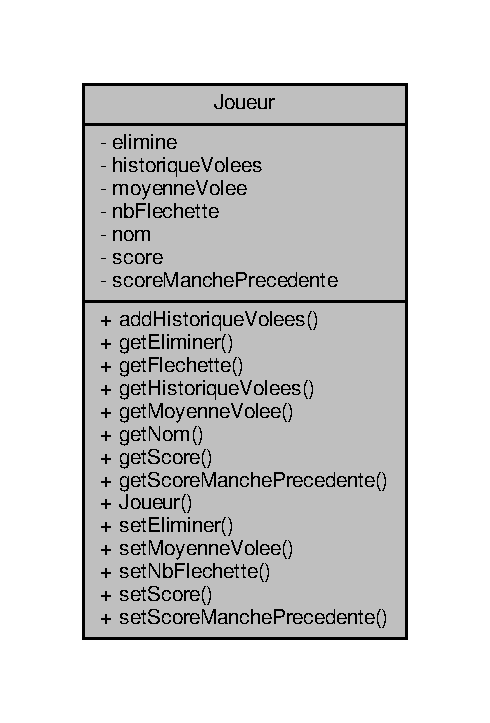
\includegraphics[width=235pt]{class_joueur__coll__graph}
\end{center}
\end{figure}
\subsubsection*{Fonctions membres publiques}
\begin{DoxyCompactItemize}
\item 
void \hyperlink{class_joueur_a219d4e16e9396f56d73485b038fc2d8f}{add\+Historique\+Volees} (float volee)
\begin{DoxyCompactList}\small\item\em Méthode qui ajoute la volée au vecteur contenant l\textquotesingle{}historique des volées. \end{DoxyCompactList}\item 
bool \hyperlink{class_joueur_abb5b33a4782973be4f5b238385c94cac}{get\+Eliminer} () const
\begin{DoxyCompactList}\small\item\em Retourne un etat true/false pour savoir si le joueur est eliminé \end{DoxyCompactList}\item 
int \hyperlink{class_joueur_a6a9730a4653b10e507c32715920bdea5}{get\+Flechette} () const
\begin{DoxyCompactList}\small\item\em Retourne le nombre de flechette du joueur. \end{DoxyCompactList}\item 
Q\+Vector$<$ float $>$ \hyperlink{class_joueur_a2f99a607d1806aae8361bbff086947f1}{get\+Historique\+Volees} () const
\begin{DoxyCompactList}\small\item\em Retourne le vector contenant tous les scores des volées precedente. \end{DoxyCompactList}\item 
int \hyperlink{class_joueur_ace9bf081d3f518eaed93b53153efcf19}{get\+Moyenne\+Volee} () const
\begin{DoxyCompactList}\small\item\em Retourne la moyenne des volees. \end{DoxyCompactList}\item 
Q\+String \hyperlink{class_joueur_a1d7082ab1f926eae1bd6834e901751a7}{get\+Nom} () const
\begin{DoxyCompactList}\small\item\em Retourne le nom du joueur. \end{DoxyCompactList}\item 
int \hyperlink{class_joueur_adf4397ffb7fcc340c2d2cc6c45edc8e2}{get\+Score} () const
\begin{DoxyCompactList}\small\item\em Retourne le score du joueur. \end{DoxyCompactList}\item 
int \hyperlink{class_joueur_ade4640f21e0f3c30390bda7d25b748fa}{get\+Score\+Manche\+Precedente} () const
\begin{DoxyCompactList}\small\item\em Retourne le score de la manche precedente. \end{DoxyCompactList}\item 
\hyperlink{class_joueur_a3832d331fb872c978f7a2d890b024b4c}{Joueur} (Q\+String \hyperlink{class_joueur_ab06d7f1e6b482299bb03919e0cd2166d}{nom}, int \hyperlink{class_joueur_a680896b9ff71c2762ae653ef6aa7c8ce}{score}, int \hyperlink{class_joueur_a330099a1952fbf97b2faea2c640b32f5}{nb\+Flechette})
\begin{DoxyCompactList}\small\item\em Constructeur de la classe \hyperlink{class_joueur}{Joueur}. \end{DoxyCompactList}\item 
void \hyperlink{class_joueur_a41dd9db4a09cd689183cc104dd1e268b}{set\+Eliminer} (bool \hyperlink{class_joueur_acac733012102f81d05b0a4c0801fcf61}{elimine})
\begin{DoxyCompactList}\small\item\em permet de modifier si le joueur est eliminer \end{DoxyCompactList}\item 
void \hyperlink{class_joueur_ab3cbde2b9f1662d47cbf4d892b11c933}{set\+Moyenne\+Volee} (int \hyperlink{class_joueur_ac5641a2a8fc1deebe5bba27bf21eb446}{moyenne\+Volee})
\begin{DoxyCompactList}\small\item\em Permets de mettre à jour la moyenne des volées. \end{DoxyCompactList}\item 
void \hyperlink{class_joueur_a3220b85c9480a2178764ef58029108aa}{set\+Nb\+Flechette} (int \hyperlink{class_joueur_a330099a1952fbf97b2faea2c640b32f5}{nb\+Flechette})
\begin{DoxyCompactList}\small\item\em Permets de mettre à jour le nombre de fléchette du joueur. \end{DoxyCompactList}\item 
void \hyperlink{class_joueur_aa7d833f3aa6058cd51a30c7e6270e696}{set\+Score} (int \hyperlink{class_joueur_a680896b9ff71c2762ae653ef6aa7c8ce}{score})
\begin{DoxyCompactList}\small\item\em Permets de mettre à jour le score du joueur. \end{DoxyCompactList}\item 
void \hyperlink{class_joueur_aaa6acb88a58bb2af33176e1468ad2107}{set\+Score\+Manche\+Precedente} (int \hyperlink{class_joueur_ac78f2e83781d2bdeb9a613dc37812736}{score\+Manche\+Precedente})
\begin{DoxyCompactList}\small\item\em Permets de mettre à jour le score de la manche précédente. \end{DoxyCompactList}\end{DoxyCompactItemize}
\subsubsection*{Attributs privés}
\begin{DoxyCompactItemize}
\item 
bool \hyperlink{class_joueur_acac733012102f81d05b0a4c0801fcf61}{elimine}
\begin{DoxyCompactList}\small\item\em contient un état true/false pour savoir si le joueur est éliminé. \end{DoxyCompactList}\item 
Q\+Vector$<$ float $>$ \hyperlink{class_joueur_aeb24d1e8125a7bf302167b91a945687e}{historique\+Volees}
\begin{DoxyCompactList}\small\item\em contient l\textquotesingle{}historique des volées du joueur \end{DoxyCompactList}\item 
int \hyperlink{class_joueur_ac5641a2a8fc1deebe5bba27bf21eb446}{moyenne\+Volee}
\begin{DoxyCompactList}\small\item\em contient la moyenne des volées du joueur \end{DoxyCompactList}\item 
int \hyperlink{class_joueur_a330099a1952fbf97b2faea2c640b32f5}{nb\+Flechette}
\begin{DoxyCompactList}\small\item\em contient le nombre de flechette restante au joueur \end{DoxyCompactList}\item 
Q\+String \hyperlink{class_joueur_ab06d7f1e6b482299bb03919e0cd2166d}{nom}
\begin{DoxyCompactList}\small\item\em contient le nom du joueur \end{DoxyCompactList}\item 
int \hyperlink{class_joueur_a680896b9ff71c2762ae653ef6aa7c8ce}{score}
\begin{DoxyCompactList}\small\item\em contient le score du joueur \end{DoxyCompactList}\item 
int \hyperlink{class_joueur_ac78f2e83781d2bdeb9a613dc37812736}{score\+Manche\+Precedente}
\begin{DoxyCompactList}\small\item\em contient le score de la manche precedente \end{DoxyCompactList}\end{DoxyCompactItemize}


\subsubsection{Description détaillée}
Déclaration de la classe \hyperlink{class_joueur}{Joueur} (Module Ecran-\/\+D\+A\+R\+TS) 

Cette classe s\textquotesingle{}occupe du stockage du nom, score et nombre de fléchettes du joueur 

Définition à la ligne \hyperlink{joueur_8h_source_l00021}{21} du fichier \hyperlink{joueur_8h_source}{joueur.\+h}.



\subsubsection{Documentation des constructeurs et destructeur}
\mbox{\Hypertarget{class_joueur_a3832d331fb872c978f7a2d890b024b4c}\label{class_joueur_a3832d331fb872c978f7a2d890b024b4c}} 
\index{Joueur@{Joueur}!Joueur@{Joueur}}
\index{Joueur@{Joueur}!Joueur@{Joueur}}
\paragraph{\texorpdfstring{Joueur()}{Joueur()}}
{\footnotesize\ttfamily Joueur\+::\+Joueur (\begin{DoxyParamCaption}\item[{Q\+String}]{nom,  }\item[{int}]{score,  }\item[{int}]{nb\+Flechette }\end{DoxyParamCaption})}



Constructeur de la classe \hyperlink{class_joueur}{Joueur}. 


\begin{DoxyParams}{Paramètres}
{\em nom} & \\
\hline
{\em score} & \\
\hline
{\em nb\+Flechette} & \\
\hline
\end{DoxyParams}


Définition à la ligne \hyperlink{joueur_8cpp_source_l00024}{24} du fichier \hyperlink{joueur_8cpp_source}{joueur.\+cpp}.



Références \hyperlink{joueur_8h_source_l00046}{nb\+Flechette}.


\begin{DoxyCode}
00024                                                       : \hyperlink{class_joueur_ab06d7f1e6b482299bb03919e0cd2166d}{nom}(\hyperlink{class_joueur_ab06d7f1e6b482299bb03919e0cd2166d}{nom}), \hyperlink{class_joueur_a680896b9ff71c2762ae653ef6aa7c8ce}{score}(
      \hyperlink{class_joueur_a680896b9ff71c2762ae653ef6aa7c8ce}{score}), \hyperlink{class_joueur_ac5641a2a8fc1deebe5bba27bf21eb446}{moyenneVolee}(0), \hyperlink{class_joueur_ac78f2e83781d2bdeb9a613dc37812736}{scoreManchePrecedente}(
      \hyperlink{class_joueur_a680896b9ff71c2762ae653ef6aa7c8ce}{score}), \hyperlink{class_joueur_a330099a1952fbf97b2faea2c640b32f5}{nbFlechette}(\hyperlink{class_joueur_a330099a1952fbf97b2faea2c640b32f5}{nbFlechette}), \hyperlink{class_joueur_acac733012102f81d05b0a4c0801fcf61}{elimine}(\textcolor{keyword}{false})
00025 \{
00026     qDebug() << Q\_FUNC\_INFO << \hyperlink{class_joueur_ab06d7f1e6b482299bb03919e0cd2166d}{nom} << \textcolor{stringliteral}{" "} << \hyperlink{class_joueur_a680896b9ff71c2762ae653ef6aa7c8ce}{score} << \textcolor{stringliteral}{" "} << \hyperlink{class_joueur_a330099a1952fbf97b2faea2c640b32f5}{nbFlechette};
00027 \}
\end{DoxyCode}


\subsubsection{Documentation des fonctions membres}
\mbox{\Hypertarget{class_joueur_a219d4e16e9396f56d73485b038fc2d8f}\label{class_joueur_a219d4e16e9396f56d73485b038fc2d8f}} 
\index{Joueur@{Joueur}!add\+Historique\+Volees@{add\+Historique\+Volees}}
\index{add\+Historique\+Volees@{add\+Historique\+Volees}!Joueur@{Joueur}}
\paragraph{\texorpdfstring{add\+Historique\+Volees()}{addHistoriqueVolees()}}
{\footnotesize\ttfamily void Joueur\+::add\+Historique\+Volees (\begin{DoxyParamCaption}\item[{float}]{volee }\end{DoxyParamCaption})}



Méthode qui ajoute la volée au vecteur contenant l\textquotesingle{}historique des volées. 


\begin{DoxyParams}{Paramètres}
{\em volee} & \\
\hline
\end{DoxyParams}


Définition à la ligne \hyperlink{joueur_8cpp_source_l00168}{168} du fichier \hyperlink{joueur_8cpp_source}{joueur.\+cpp}.



Références \hyperlink{joueur_8h_source_l00042}{historique\+Volees}.


\begin{DoxyCode}
00169 \{
00170     \hyperlink{class_joueur_aeb24d1e8125a7bf302167b91a945687e}{historiqueVolees}.push\_back(volee);
00171 \}
\end{DoxyCode}
\mbox{\Hypertarget{class_joueur_abb5b33a4782973be4f5b238385c94cac}\label{class_joueur_abb5b33a4782973be4f5b238385c94cac}} 
\index{Joueur@{Joueur}!get\+Eliminer@{get\+Eliminer}}
\index{get\+Eliminer@{get\+Eliminer}!Joueur@{Joueur}}
\paragraph{\texorpdfstring{get\+Eliminer()}{getEliminer()}}
{\footnotesize\ttfamily bool Joueur\+::get\+Eliminer (\begin{DoxyParamCaption}{ }\end{DoxyParamCaption}) const}



Retourne un etat true/false pour savoir si le joueur est eliminé 

\begin{DoxyReturn}{Renvoie}
bool 
\end{DoxyReturn}


Définition à la ligne \hyperlink{joueur_8cpp_source_l00101}{101} du fichier \hyperlink{joueur_8cpp_source}{joueur.\+cpp}.



Références \hyperlink{joueur_8h_source_l00047}{elimine}.


\begin{DoxyCode}
00102 \{
00103     \textcolor{keywordflow}{return} this->\hyperlink{class_joueur_acac733012102f81d05b0a4c0801fcf61}{elimine};
00104 \}
\end{DoxyCode}
\mbox{\Hypertarget{class_joueur_a6a9730a4653b10e507c32715920bdea5}\label{class_joueur_a6a9730a4653b10e507c32715920bdea5}} 
\index{Joueur@{Joueur}!get\+Flechette@{get\+Flechette}}
\index{get\+Flechette@{get\+Flechette}!Joueur@{Joueur}}
\paragraph{\texorpdfstring{get\+Flechette()}{getFlechette()}}
{\footnotesize\ttfamily int Joueur\+::get\+Flechette (\begin{DoxyParamCaption}{ }\end{DoxyParamCaption}) const}



Retourne le nombre de flechette du joueur. 

\begin{DoxyReturn}{Renvoie}
int 
\end{DoxyReturn}


Définition à la ligne \hyperlink{joueur_8cpp_source_l00068}{68} du fichier \hyperlink{joueur_8cpp_source}{joueur.\+cpp}.



Références \hyperlink{joueur_8h_source_l00046}{nb\+Flechette}.


\begin{DoxyCode}
00069 \{
00070     \textcolor{keywordflow}{return} this->\hyperlink{class_joueur_a330099a1952fbf97b2faea2c640b32f5}{nbFlechette};
00071 \}
\end{DoxyCode}
\mbox{\Hypertarget{class_joueur_a2f99a607d1806aae8361bbff086947f1}\label{class_joueur_a2f99a607d1806aae8361bbff086947f1}} 
\index{Joueur@{Joueur}!get\+Historique\+Volees@{get\+Historique\+Volees}}
\index{get\+Historique\+Volees@{get\+Historique\+Volees}!Joueur@{Joueur}}
\paragraph{\texorpdfstring{get\+Historique\+Volees()}{getHistoriqueVolees()}}
{\footnotesize\ttfamily Q\+Vector$<$ float $>$ Joueur\+::get\+Historique\+Volees (\begin{DoxyParamCaption}{ }\end{DoxyParamCaption}) const}



Retourne le vector contenant tous les scores des volées precedente. 

\begin{DoxyReturn}{Renvoie}
Q\+Vector$<$float$>$ 
\end{DoxyReturn}


Définition à la ligne \hyperlink{joueur_8cpp_source_l00090}{90} du fichier \hyperlink{joueur_8cpp_source}{joueur.\+cpp}.



Références \hyperlink{joueur_8h_source_l00042}{historique\+Volees}.


\begin{DoxyCode}
00091 \{
00092     \textcolor{keywordflow}{return} this->\hyperlink{class_joueur_aeb24d1e8125a7bf302167b91a945687e}{historiqueVolees};
00093 \}
\end{DoxyCode}
\mbox{\Hypertarget{class_joueur_ace9bf081d3f518eaed93b53153efcf19}\label{class_joueur_ace9bf081d3f518eaed93b53153efcf19}} 
\index{Joueur@{Joueur}!get\+Moyenne\+Volee@{get\+Moyenne\+Volee}}
\index{get\+Moyenne\+Volee@{get\+Moyenne\+Volee}!Joueur@{Joueur}}
\paragraph{\texorpdfstring{get\+Moyenne\+Volee()}{getMoyenneVolee()}}
{\footnotesize\ttfamily int Joueur\+::get\+Moyenne\+Volee (\begin{DoxyParamCaption}{ }\end{DoxyParamCaption}) const}



Retourne la moyenne des volees. 

\begin{DoxyReturn}{Renvoie}
float 
\end{DoxyReturn}


Définition à la ligne \hyperlink{joueur_8cpp_source_l00079}{79} du fichier \hyperlink{joueur_8cpp_source}{joueur.\+cpp}.



Références \hyperlink{joueur_8h_source_l00044}{moyenne\+Volee}.


\begin{DoxyCode}
00080 \{
00081     \textcolor{keywordflow}{return} this->\hyperlink{class_joueur_ac5641a2a8fc1deebe5bba27bf21eb446}{moyenneVolee};
00082 \}
\end{DoxyCode}
\mbox{\Hypertarget{class_joueur_a1d7082ab1f926eae1bd6834e901751a7}\label{class_joueur_a1d7082ab1f926eae1bd6834e901751a7}} 
\index{Joueur@{Joueur}!get\+Nom@{get\+Nom}}
\index{get\+Nom@{get\+Nom}!Joueur@{Joueur}}
\paragraph{\texorpdfstring{get\+Nom()}{getNom()}}
{\footnotesize\ttfamily Q\+String Joueur\+::get\+Nom (\begin{DoxyParamCaption}{ }\end{DoxyParamCaption}) const}



Retourne le nom du joueur. 

\begin{DoxyReturn}{Renvoie}
Q\+String 
\end{DoxyReturn}


Définition à la ligne \hyperlink{joueur_8cpp_source_l00035}{35} du fichier \hyperlink{joueur_8cpp_source}{joueur.\+cpp}.



Références \hyperlink{joueur_8h_source_l00041}{nom}.


\begin{DoxyCode}
00036 \{
00037     \textcolor{keywordflow}{return} this->\hyperlink{class_joueur_ab06d7f1e6b482299bb03919e0cd2166d}{nom};
00038 \}
\end{DoxyCode}
\mbox{\Hypertarget{class_joueur_adf4397ffb7fcc340c2d2cc6c45edc8e2}\label{class_joueur_adf4397ffb7fcc340c2d2cc6c45edc8e2}} 
\index{Joueur@{Joueur}!get\+Score@{get\+Score}}
\index{get\+Score@{get\+Score}!Joueur@{Joueur}}
\paragraph{\texorpdfstring{get\+Score()}{getScore()}}
{\footnotesize\ttfamily int Joueur\+::get\+Score (\begin{DoxyParamCaption}{ }\end{DoxyParamCaption}) const}



Retourne le score du joueur. 

\begin{DoxyReturn}{Renvoie}
int 
\end{DoxyReturn}


Définition à la ligne \hyperlink{joueur_8cpp_source_l00046}{46} du fichier \hyperlink{joueur_8cpp_source}{joueur.\+cpp}.



Références \hyperlink{joueur_8h_source_l00043}{score}.


\begin{DoxyCode}
00047 \{
00048     \textcolor{keywordflow}{return} this->\hyperlink{class_joueur_a680896b9ff71c2762ae653ef6aa7c8ce}{score};
00049 \}
\end{DoxyCode}
\mbox{\Hypertarget{class_joueur_ade4640f21e0f3c30390bda7d25b748fa}\label{class_joueur_ade4640f21e0f3c30390bda7d25b748fa}} 
\index{Joueur@{Joueur}!get\+Score\+Manche\+Precedente@{get\+Score\+Manche\+Precedente}}
\index{get\+Score\+Manche\+Precedente@{get\+Score\+Manche\+Precedente}!Joueur@{Joueur}}
\paragraph{\texorpdfstring{get\+Score\+Manche\+Precedente()}{getScoreManchePrecedente()}}
{\footnotesize\ttfamily int Joueur\+::get\+Score\+Manche\+Precedente (\begin{DoxyParamCaption}{ }\end{DoxyParamCaption}) const}



Retourne le score de la manche precedente. 

\begin{DoxyReturn}{Renvoie}
int 
\end{DoxyReturn}


Définition à la ligne \hyperlink{joueur_8cpp_source_l00057}{57} du fichier \hyperlink{joueur_8cpp_source}{joueur.\+cpp}.



Références \hyperlink{joueur_8h_source_l00045}{score\+Manche\+Precedente}.


\begin{DoxyCode}
00058 \{
00059     \textcolor{keywordflow}{return} this->\hyperlink{class_joueur_ac78f2e83781d2bdeb9a613dc37812736}{scoreManchePrecedente};
00060 \}
\end{DoxyCode}
\mbox{\Hypertarget{class_joueur_a41dd9db4a09cd689183cc104dd1e268b}\label{class_joueur_a41dd9db4a09cd689183cc104dd1e268b}} 
\index{Joueur@{Joueur}!set\+Eliminer@{set\+Eliminer}}
\index{set\+Eliminer@{set\+Eliminer}!Joueur@{Joueur}}
\paragraph{\texorpdfstring{set\+Eliminer()}{setEliminer()}}
{\footnotesize\ttfamily void Joueur\+::set\+Eliminer (\begin{DoxyParamCaption}\item[{bool}]{elimine }\end{DoxyParamCaption})}



permet de modifier si le joueur est eliminer 


\begin{DoxyParams}{Paramètres}
{\em elimine} & \\
\hline
\end{DoxyParams}


Définition à la ligne \hyperlink{joueur_8cpp_source_l00112}{112} du fichier \hyperlink{joueur_8cpp_source}{joueur.\+cpp}.



Références \hyperlink{joueur_8h_source_l00047}{elimine}.


\begin{DoxyCode}
00113 \{
00114     this->\hyperlink{class_joueur_acac733012102f81d05b0a4c0801fcf61}{elimine} = \hyperlink{class_joueur_acac733012102f81d05b0a4c0801fcf61}{elimine};
00115 \}
\end{DoxyCode}
\mbox{\Hypertarget{class_joueur_ab3cbde2b9f1662d47cbf4d892b11c933}\label{class_joueur_ab3cbde2b9f1662d47cbf4d892b11c933}} 
\index{Joueur@{Joueur}!set\+Moyenne\+Volee@{set\+Moyenne\+Volee}}
\index{set\+Moyenne\+Volee@{set\+Moyenne\+Volee}!Joueur@{Joueur}}
\paragraph{\texorpdfstring{set\+Moyenne\+Volee()}{setMoyenneVolee()}}
{\footnotesize\ttfamily void Joueur\+::set\+Moyenne\+Volee (\begin{DoxyParamCaption}\item[{int}]{moyenne\+Volee }\end{DoxyParamCaption})}



Permets de mettre à jour la moyenne des volées. 


\begin{DoxyParams}{Paramètres}
{\em moyenne\+Volee} & \\
\hline
\end{DoxyParams}


Définition à la ligne \hyperlink{joueur_8cpp_source_l00123}{123} du fichier \hyperlink{joueur_8cpp_source}{joueur.\+cpp}.



Références \hyperlink{joueur_8h_source_l00044}{moyenne\+Volee}.


\begin{DoxyCode}
00124 \{
00125     this->\hyperlink{class_joueur_ac5641a2a8fc1deebe5bba27bf21eb446}{moyenneVolee} = \hyperlink{class_joueur_ac5641a2a8fc1deebe5bba27bf21eb446}{moyenneVolee};
00126 \}
\end{DoxyCode}
\mbox{\Hypertarget{class_joueur_a3220b85c9480a2178764ef58029108aa}\label{class_joueur_a3220b85c9480a2178764ef58029108aa}} 
\index{Joueur@{Joueur}!set\+Nb\+Flechette@{set\+Nb\+Flechette}}
\index{set\+Nb\+Flechette@{set\+Nb\+Flechette}!Joueur@{Joueur}}
\paragraph{\texorpdfstring{set\+Nb\+Flechette()}{setNbFlechette()}}
{\footnotesize\ttfamily void Joueur\+::set\+Nb\+Flechette (\begin{DoxyParamCaption}\item[{int}]{nb\+Flechette }\end{DoxyParamCaption})}



Permets de mettre à jour le nombre de fléchette du joueur. 


\begin{DoxyParams}{Paramètres}
{\em nb\+Flechette} & \\
\hline
\end{DoxyParams}


Définition à la ligne \hyperlink{joueur_8cpp_source_l00157}{157} du fichier \hyperlink{joueur_8cpp_source}{joueur.\+cpp}.



Références \hyperlink{joueur_8h_source_l00046}{nb\+Flechette}.


\begin{DoxyCode}
00158 \{
00159     this->\hyperlink{class_joueur_a330099a1952fbf97b2faea2c640b32f5}{nbFlechette} = \hyperlink{class_joueur_a330099a1952fbf97b2faea2c640b32f5}{nbFlechette};
00160 \}
\end{DoxyCode}
\mbox{\Hypertarget{class_joueur_aa7d833f3aa6058cd51a30c7e6270e696}\label{class_joueur_aa7d833f3aa6058cd51a30c7e6270e696}} 
\index{Joueur@{Joueur}!set\+Score@{set\+Score}}
\index{set\+Score@{set\+Score}!Joueur@{Joueur}}
\paragraph{\texorpdfstring{set\+Score()}{setScore()}}
{\footnotesize\ttfamily void Joueur\+::set\+Score (\begin{DoxyParamCaption}\item[{int}]{score }\end{DoxyParamCaption})}



Permets de mettre à jour le score du joueur. 


\begin{DoxyParams}{Paramètres}
{\em score} & \\
\hline
\end{DoxyParams}


Définition à la ligne \hyperlink{joueur_8cpp_source_l00135}{135} du fichier \hyperlink{joueur_8cpp_source}{joueur.\+cpp}.



Références \hyperlink{joueur_8h_source_l00043}{score}.


\begin{DoxyCode}
00136 \{
00137     this->\hyperlink{class_joueur_a680896b9ff71c2762ae653ef6aa7c8ce}{score} = \hyperlink{class_joueur_a680896b9ff71c2762ae653ef6aa7c8ce}{score};
00138 \}
\end{DoxyCode}
\mbox{\Hypertarget{class_joueur_aaa6acb88a58bb2af33176e1468ad2107}\label{class_joueur_aaa6acb88a58bb2af33176e1468ad2107}} 
\index{Joueur@{Joueur}!set\+Score\+Manche\+Precedente@{set\+Score\+Manche\+Precedente}}
\index{set\+Score\+Manche\+Precedente@{set\+Score\+Manche\+Precedente}!Joueur@{Joueur}}
\paragraph{\texorpdfstring{set\+Score\+Manche\+Precedente()}{setScoreManchePrecedente()}}
{\footnotesize\ttfamily void Joueur\+::set\+Score\+Manche\+Precedente (\begin{DoxyParamCaption}\item[{int}]{score\+Manche\+Precedente }\end{DoxyParamCaption})}



Permets de mettre à jour le score de la manche précédente. 


\begin{DoxyParams}{Paramètres}
{\em score\+Manche\+Precedente} & \\
\hline
\end{DoxyParams}


Définition à la ligne \hyperlink{joueur_8cpp_source_l00146}{146} du fichier \hyperlink{joueur_8cpp_source}{joueur.\+cpp}.



Références \hyperlink{joueur_8h_source_l00045}{score\+Manche\+Precedente}.


\begin{DoxyCode}
00147 \{
00148     this->\hyperlink{class_joueur_ac78f2e83781d2bdeb9a613dc37812736}{scoreManchePrecedente} = \hyperlink{class_joueur_ac78f2e83781d2bdeb9a613dc37812736}{scoreManchePrecedente};
00149 \}
\end{DoxyCode}


\subsubsection{Documentation des données membres}
\mbox{\Hypertarget{class_joueur_acac733012102f81d05b0a4c0801fcf61}\label{class_joueur_acac733012102f81d05b0a4c0801fcf61}} 
\index{Joueur@{Joueur}!elimine@{elimine}}
\index{elimine@{elimine}!Joueur@{Joueur}}
\paragraph{\texorpdfstring{elimine}{elimine}}
{\footnotesize\ttfamily bool Joueur\+::elimine\hspace{0.3cm}{\ttfamily [private]}}



contient un état true/false pour savoir si le joueur est éliminé. 



Définition à la ligne \hyperlink{joueur_8h_source_l00047}{47} du fichier \hyperlink{joueur_8h_source}{joueur.\+h}.



Référencé par \hyperlink{joueur_8cpp_source_l00101}{get\+Eliminer()}, et \hyperlink{joueur_8cpp_source_l00112}{set\+Eliminer()}.

\mbox{\Hypertarget{class_joueur_aeb24d1e8125a7bf302167b91a945687e}\label{class_joueur_aeb24d1e8125a7bf302167b91a945687e}} 
\index{Joueur@{Joueur}!historique\+Volees@{historique\+Volees}}
\index{historique\+Volees@{historique\+Volees}!Joueur@{Joueur}}
\paragraph{\texorpdfstring{historique\+Volees}{historiqueVolees}}
{\footnotesize\ttfamily Q\+Vector$<$float$>$ Joueur\+::historique\+Volees\hspace{0.3cm}{\ttfamily [private]}}



contient l\textquotesingle{}historique des volées du joueur 



Définition à la ligne \hyperlink{joueur_8h_source_l00042}{42} du fichier \hyperlink{joueur_8h_source}{joueur.\+h}.



Référencé par \hyperlink{joueur_8cpp_source_l00168}{add\+Historique\+Volees()}, et \hyperlink{joueur_8cpp_source_l00090}{get\+Historique\+Volees()}.

\mbox{\Hypertarget{class_joueur_ac5641a2a8fc1deebe5bba27bf21eb446}\label{class_joueur_ac5641a2a8fc1deebe5bba27bf21eb446}} 
\index{Joueur@{Joueur}!moyenne\+Volee@{moyenne\+Volee}}
\index{moyenne\+Volee@{moyenne\+Volee}!Joueur@{Joueur}}
\paragraph{\texorpdfstring{moyenne\+Volee}{moyenneVolee}}
{\footnotesize\ttfamily int Joueur\+::moyenne\+Volee\hspace{0.3cm}{\ttfamily [private]}}



contient la moyenne des volées du joueur 



Définition à la ligne \hyperlink{joueur_8h_source_l00044}{44} du fichier \hyperlink{joueur_8h_source}{joueur.\+h}.



Référencé par \hyperlink{joueur_8cpp_source_l00079}{get\+Moyenne\+Volee()}, et \hyperlink{joueur_8cpp_source_l00123}{set\+Moyenne\+Volee()}.

\mbox{\Hypertarget{class_joueur_a330099a1952fbf97b2faea2c640b32f5}\label{class_joueur_a330099a1952fbf97b2faea2c640b32f5}} 
\index{Joueur@{Joueur}!nb\+Flechette@{nb\+Flechette}}
\index{nb\+Flechette@{nb\+Flechette}!Joueur@{Joueur}}
\paragraph{\texorpdfstring{nb\+Flechette}{nbFlechette}}
{\footnotesize\ttfamily int Joueur\+::nb\+Flechette\hspace{0.3cm}{\ttfamily [private]}}



contient le nombre de flechette restante au joueur 



Définition à la ligne \hyperlink{joueur_8h_source_l00046}{46} du fichier \hyperlink{joueur_8h_source}{joueur.\+h}.



Référencé par \hyperlink{joueur_8cpp_source_l00068}{get\+Flechette()}, \hyperlink{joueur_8cpp_source_l00024}{Joueur()}, et \hyperlink{joueur_8cpp_source_l00157}{set\+Nb\+Flechette()}.

\mbox{\Hypertarget{class_joueur_ab06d7f1e6b482299bb03919e0cd2166d}\label{class_joueur_ab06d7f1e6b482299bb03919e0cd2166d}} 
\index{Joueur@{Joueur}!nom@{nom}}
\index{nom@{nom}!Joueur@{Joueur}}
\paragraph{\texorpdfstring{nom}{nom}}
{\footnotesize\ttfamily Q\+String Joueur\+::nom\hspace{0.3cm}{\ttfamily [private]}}



contient le nom du joueur 



Définition à la ligne \hyperlink{joueur_8h_source_l00041}{41} du fichier \hyperlink{joueur_8h_source}{joueur.\+h}.



Référencé par \hyperlink{joueur_8cpp_source_l00035}{get\+Nom()}.

\mbox{\Hypertarget{class_joueur_a680896b9ff71c2762ae653ef6aa7c8ce}\label{class_joueur_a680896b9ff71c2762ae653ef6aa7c8ce}} 
\index{Joueur@{Joueur}!score@{score}}
\index{score@{score}!Joueur@{Joueur}}
\paragraph{\texorpdfstring{score}{score}}
{\footnotesize\ttfamily int Joueur\+::score\hspace{0.3cm}{\ttfamily [private]}}



contient le score du joueur 



Définition à la ligne \hyperlink{joueur_8h_source_l00043}{43} du fichier \hyperlink{joueur_8h_source}{joueur.\+h}.



Référencé par \hyperlink{joueur_8cpp_source_l00046}{get\+Score()}, et \hyperlink{joueur_8cpp_source_l00135}{set\+Score()}.

\mbox{\Hypertarget{class_joueur_ac78f2e83781d2bdeb9a613dc37812736}\label{class_joueur_ac78f2e83781d2bdeb9a613dc37812736}} 
\index{Joueur@{Joueur}!score\+Manche\+Precedente@{score\+Manche\+Precedente}}
\index{score\+Manche\+Precedente@{score\+Manche\+Precedente}!Joueur@{Joueur}}
\paragraph{\texorpdfstring{score\+Manche\+Precedente}{scoreManchePrecedente}}
{\footnotesize\ttfamily int Joueur\+::score\+Manche\+Precedente\hspace{0.3cm}{\ttfamily [private]}}



contient le score de la manche precedente 



Définition à la ligne \hyperlink{joueur_8h_source_l00045}{45} du fichier \hyperlink{joueur_8h_source}{joueur.\+h}.



Référencé par \hyperlink{joueur_8cpp_source_l00057}{get\+Score\+Manche\+Precedente()}, et \hyperlink{joueur_8cpp_source_l00146}{set\+Score\+Manche\+Precedente()}.



La documentation de cette classe a été générée à partir des fichiers suivants \+:\begin{DoxyCompactItemize}
\item 
\hyperlink{joueur_8h}{joueur.\+h}\item 
\hyperlink{joueur_8cpp}{joueur.\+cpp}\end{DoxyCompactItemize}

\hypertarget{class_q_object}{}\subsection{Référence de la classe Q\+Object}
\label{class_q_object}\index{Q\+Object@{Q\+Object}}


La classe \hyperlink{class_q_object}{Q\+Object} est la classe de base de tous les objets Qt. Elle permet à ces objets Qt de disposer entre autres du mécanisme de communication signal/slot.  




Graphe de collaboration de Q\+Object\+:\nopagebreak
\begin{figure}[H]
\begin{center}
\leavevmode
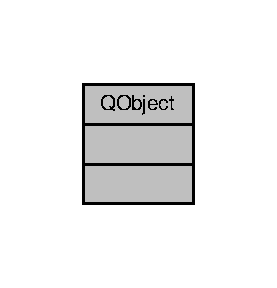
\includegraphics[width=133pt]{class_q_object__coll__graph}
\end{center}
\end{figure}


\subsubsection{Description détaillée}
La classe \hyperlink{class_q_object}{Q\+Object} est la classe de base de tous les objets Qt. Elle permet à ces objets Qt de disposer entre autres du mécanisme de communication signal/slot. 

La documentation de cette classe a été générée à partir du fichier suivant \+:\begin{DoxyCompactItemize}
\item 
\hyperlink{main_8cpp}{main.\+cpp}\end{DoxyCompactItemize}

\hypertarget{class_q_widget}{}\subsection{Référence de la classe Q\+Widget}
\label{class_q_widget}\index{Q\+Widget@{Q\+Widget}}


La classe \hyperlink{class_q_widget}{Q\+Widget} est la classe de base de tous les objets graphiques d\textquotesingle{}interface utilisateur.  




Graphe de collaboration de Q\+Widget\+:\nopagebreak
\begin{figure}[H]
\begin{center}
\leavevmode
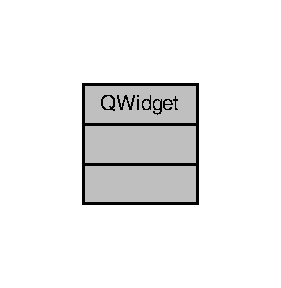
\includegraphics[width=135pt]{class_q_widget__coll__graph}
\end{center}
\end{figure}


\subsubsection{Description détaillée}
La classe \hyperlink{class_q_widget}{Q\+Widget} est la classe de base de tous les objets graphiques d\textquotesingle{}interface utilisateur. 

La documentation de cette classe a été générée à partir du fichier suivant \+:\begin{DoxyCompactItemize}
\item 
\hyperlink{main_8cpp}{main.\+cpp}\end{DoxyCompactItemize}

\hypertarget{class_solution}{}\subsection{Référence de la classe Solution}
\label{class_solution}\index{Solution@{Solution}}


Déclaration de la classe \hyperlink{class_solution}{Solution} (Module Ecran-\/\+D\+A\+R\+TS)  




{\ttfamily \#include $<$solution.\+h$>$}



Graphe de collaboration de Solution\+:
\nopagebreak
\begin{figure}[H]
\begin{center}
\leavevmode
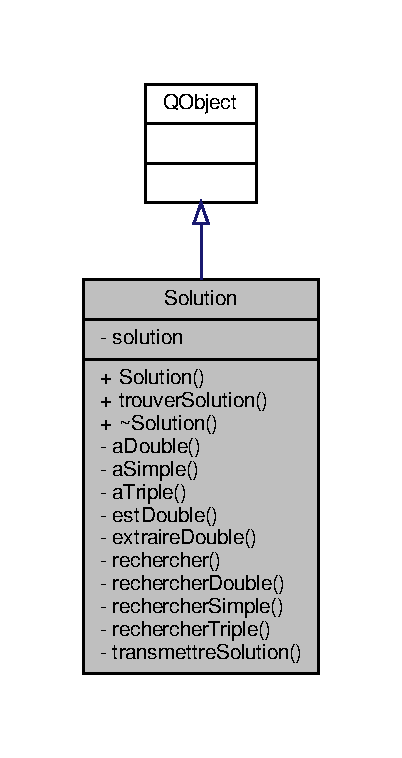
\includegraphics[width=193pt]{class_solution__coll__graph}
\end{center}
\end{figure}
\subsubsection*{Signaux}
\begin{DoxyCompactItemize}
\item 
void \hyperlink{class_solution_a052b7ba921e7b211d14f2bbbc6b63832}{solution\+Trouver} (Q\+String \hyperlink{class_solution_a03b47dedfe8a8f8244f7e633cbaa30fb}{solution})
\end{DoxyCompactItemize}
\subsubsection*{Fonctions membres publiques}
\begin{DoxyCompactItemize}
\item 
\hyperlink{class_solution_a378d4a570c95a6d4c013996fef75c6f0}{Solution} (\hyperlink{class_q_object}{Q\+Object} $\ast$parent=nullptr)
\begin{DoxyCompactList}\small\item\em Constructeur de la classe \hyperlink{class_solution}{Solution}. \end{DoxyCompactList}\item 
void \hyperlink{class_solution_a9ab0b0fd2b557f5abda8bd1a6da641e4}{trouver\+Solution} (int s, int flechettes)
\begin{DoxyCompactList}\small\item\em Méthode qui trouve la meilleure solution. \end{DoxyCompactList}\item 
\hyperlink{class_solution_a5d245f7409aacf6ace5e965b7879a580}{$\sim$\+Solution} ()
\begin{DoxyCompactList}\small\item\em Destructeur de la classe \hyperlink{class_solution}{Solution}. \end{DoxyCompactList}\end{DoxyCompactItemize}
\subsubsection*{Fonctions membres privées}
\begin{DoxyCompactItemize}
\item 
bool \hyperlink{class_solution_ad79929c887a394883a154ea2ca9c3aac}{a\+Double} (int points, const int score)
\begin{DoxyCompactList}\small\item\em Test si le double choisie et possible. \end{DoxyCompactList}\item 
bool \hyperlink{class_solution_a932ab2aea629d049202e8f8e38cc01b3}{a\+Simple} (int points, const int score)
\begin{DoxyCompactList}\small\item\em Test si le simple choisi et possible. \end{DoxyCompactList}\item 
bool \hyperlink{class_solution_af8062e8e2997f8a7451e439ce23dd544}{a\+Triple} (int points, const int score)
\begin{DoxyCompactList}\small\item\em Test si la triple choisie et possible. \end{DoxyCompactList}\item 
bool \hyperlink{class_solution_add9d51c9612fa89361df0908e10779b8}{est\+Double} (int points, const int score)
\begin{DoxyCompactList}\small\item\em Méthode qui teste si les points son double. \end{DoxyCompactList}\item 
bool \hyperlink{class_solution_a34c3bf5ce00cdf428f2e07741806499d}{extraire\+Double} (int \&score, int cible)
\begin{DoxyCompactList}\small\item\em Méthode qui cherche le double pour finir la partie. \end{DoxyCompactList}\item 
bool \hyperlink{class_solution_a857b1b362fc0d5eb08e2eb7302dce27f}{rechercher} (int score, int nb\+Flechettes, bool still=false)
\begin{DoxyCompactList}\small\item\em Méthode qui recherche la meilleure combinaison pour finir. \end{DoxyCompactList}\item 
bool \hyperlink{class_solution_aa54574bee5bde60d55a9da346a61cf48}{rechercher\+Double} (int \&score, Q\+String \&combinaison)
\begin{DoxyCompactList}\small\item\em Méthode qui recherche le meilleur double pour la solution. \end{DoxyCompactList}\item 
bool \hyperlink{class_solution_ab8223455a5a35aceb7de18970f94db48}{rechercher\+Simple} (int \&score, Q\+String \&combinaison)
\begin{DoxyCompactList}\small\item\em Méthode qui recherche le meilleur simple pour la solution. \end{DoxyCompactList}\item 
bool \hyperlink{class_solution_a7f3302e8292858a51795f08751d54ef9}{rechercher\+Triple} (int \&score, Q\+String \&combinaison, int start)
\begin{DoxyCompactList}\small\item\em Méthode qui recherche le meilleur triple pour la solution. \end{DoxyCompactList}\item 
void \hyperlink{class_solution_a334ffddf70bd379a0af7c7e93750d6b5}{transmettre\+Solution} (int score)
\begin{DoxyCompactList}\small\item\em Méthode qui émet un signal pour que l\textquotesingle{}\hyperlink{class_ihm}{Ihm} affiche la solution trouver. \end{DoxyCompactList}\end{DoxyCompactItemize}
\subsubsection*{Attributs privés}
\begin{DoxyCompactItemize}
\item 
Q\+String \hyperlink{class_solution_a03b47dedfe8a8f8244f7e633cbaa30fb}{solution}
\begin{DoxyCompactList}\small\item\em contient la solution pour finir la partie \end{DoxyCompactList}\end{DoxyCompactItemize}


\subsubsection{Description détaillée}
Déclaration de la classe \hyperlink{class_solution}{Solution} (Module Ecran-\/\+D\+A\+R\+TS) 

Cette classe s\textquotesingle{}occupe de rechercher les différentes solutions pour finir la partie 

Définition à la ligne \hyperlink{solution_8h_source_l00030}{30} du fichier \hyperlink{solution_8h_source}{solution.\+h}.



\subsubsection{Documentation des constructeurs et destructeur}
\mbox{\Hypertarget{class_solution_a378d4a570c95a6d4c013996fef75c6f0}\label{class_solution_a378d4a570c95a6d4c013996fef75c6f0}} 
\index{Solution@{Solution}!Solution@{Solution}}
\index{Solution@{Solution}!Solution@{Solution}}
\paragraph{\texorpdfstring{Solution()}{Solution()}}
{\footnotesize\ttfamily Solution\+::\+Solution (\begin{DoxyParamCaption}\item[{\hyperlink{class_q_object}{Q\+Object} $\ast$}]{parent = {\ttfamily nullptr} }\end{DoxyParamCaption})\hspace{0.3cm}{\ttfamily [explicit]}}



Constructeur de la classe \hyperlink{class_solution}{Solution}. 


\begin{DoxyParams}{Paramètres}
{\em parent} & \\
\hline
\end{DoxyParams}


Définition à la ligne \hyperlink{solution_8cpp_source_l00020}{20} du fichier \hyperlink{solution_8cpp_source}{solution.\+cpp}.


\begin{DoxyCode}
00020                                   : \hyperlink{class_q_object}{QObject}(parent), \hyperlink{class_solution_a03b47dedfe8a8f8244f7e633cbaa30fb}{solution}(\textcolor{stringliteral}{""})
00021 \{
00022    qDebug() << Q\_FUNC\_INFO;
00023 \}
\end{DoxyCode}
\mbox{\Hypertarget{class_solution_a5d245f7409aacf6ace5e965b7879a580}\label{class_solution_a5d245f7409aacf6ace5e965b7879a580}} 
\index{Solution@{Solution}!````~Solution@{$\sim$\+Solution}}
\index{````~Solution@{$\sim$\+Solution}!Solution@{Solution}}
\paragraph{\texorpdfstring{$\sim$\+Solution()}{~Solution()}}
{\footnotesize\ttfamily Solution\+::$\sim$\+Solution (\begin{DoxyParamCaption}{ }\end{DoxyParamCaption})}



Destructeur de la classe \hyperlink{class_solution}{Solution}. 



Définition à la ligne \hyperlink{solution_8cpp_source_l00030}{30} du fichier \hyperlink{solution_8cpp_source}{solution.\+cpp}.


\begin{DoxyCode}
00031 \{
00032    qDebug() << Q\_FUNC\_INFO;
00033 \}
\end{DoxyCode}


\subsubsection{Documentation des fonctions membres}
\mbox{\Hypertarget{class_solution_ad79929c887a394883a154ea2ca9c3aac}\label{class_solution_ad79929c887a394883a154ea2ca9c3aac}} 
\index{Solution@{Solution}!a\+Double@{a\+Double}}
\index{a\+Double@{a\+Double}!Solution@{Solution}}
\paragraph{\texorpdfstring{a\+Double()}{aDouble()}}
{\footnotesize\ttfamily bool Solution\+::a\+Double (\begin{DoxyParamCaption}\item[{int}]{points,  }\item[{const int}]{score }\end{DoxyParamCaption})\hspace{0.3cm}{\ttfamily [private]}}



Test si le double choisie et possible. 


\begin{DoxyParams}{Paramètres}
{\em points} & \\
\hline
{\em score} & \\
\hline
\end{DoxyParams}
\begin{DoxyReturn}{Renvoie}
bool 
\end{DoxyReturn}


Définition à la ligne \hyperlink{solution_8cpp_source_l00097}{97} du fichier \hyperlink{solution_8cpp_source}{solution.\+cpp}.



Référencé par \hyperlink{solution_8cpp_source_l00198}{extraire\+Double()}, et \hyperlink{solution_8cpp_source_l00114}{rechercher\+Double()}.


\begin{DoxyCode}
00098 \{
00099     \textcolor{keywordflow}{if}((score / (points*2)) >= 1)
00100     \{
00101         \textcolor{keywordflow}{return} \textcolor{keyword}{true};
00102     \}
00103     \textcolor{keywordflow}{return} \textcolor{keyword}{false};
00104 \}
\end{DoxyCode}
\mbox{\Hypertarget{class_solution_a932ab2aea629d049202e8f8e38cc01b3}\label{class_solution_a932ab2aea629d049202e8f8e38cc01b3}} 
\index{Solution@{Solution}!a\+Simple@{a\+Simple}}
\index{a\+Simple@{a\+Simple}!Solution@{Solution}}
\paragraph{\texorpdfstring{a\+Simple()}{aSimple()}}
{\footnotesize\ttfamily bool Solution\+::a\+Simple (\begin{DoxyParamCaption}\item[{int}]{points,  }\item[{const int}]{score }\end{DoxyParamCaption})\hspace{0.3cm}{\ttfamily [private]}}



Test si le simple choisi et possible. 


\begin{DoxyParams}{Paramètres}
{\em points} & \\
\hline
{\em score} & \\
\hline
\end{DoxyParams}
\begin{DoxyReturn}{Renvoie}
bool 
\end{DoxyReturn}


Définition à la ligne \hyperlink{solution_8cpp_source_l00141}{141} du fichier \hyperlink{solution_8cpp_source}{solution.\+cpp}.



Référencé par \hyperlink{solution_8cpp_source_l00156}{rechercher\+Simple()}.


\begin{DoxyCode}
00142 \{
00143     \textcolor{keywordflow}{if}((score / points) >= 1)
00144         \textcolor{keywordflow}{return} \textcolor{keyword}{true};
00145     \textcolor{keywordflow}{return} \textcolor{keyword}{false};
00146 \}
\end{DoxyCode}
\mbox{\Hypertarget{class_solution_af8062e8e2997f8a7451e439ce23dd544}\label{class_solution_af8062e8e2997f8a7451e439ce23dd544}} 
\index{Solution@{Solution}!a\+Triple@{a\+Triple}}
\index{a\+Triple@{a\+Triple}!Solution@{Solution}}
\paragraph{\texorpdfstring{a\+Triple()}{aTriple()}}
{\footnotesize\ttfamily bool Solution\+::a\+Triple (\begin{DoxyParamCaption}\item[{int}]{points,  }\item[{const int}]{score }\end{DoxyParamCaption})\hspace{0.3cm}{\ttfamily [private]}}



Test si la triple choisie et possible. 


\begin{DoxyParams}{Paramètres}
{\em points} & \\
\hline
{\em score} & \\
\hline
\end{DoxyParams}
\begin{DoxyReturn}{Renvoie}
bool 
\end{DoxyReturn}


Définition à la ligne \hyperlink{solution_8cpp_source_l00056}{56} du fichier \hyperlink{solution_8cpp_source}{solution.\+cpp}.



Référencé par \hyperlink{solution_8cpp_source_l00074}{rechercher\+Triple()}.


\begin{DoxyCode}
00057 \{
00058     \textcolor{keywordflow}{if}((score / (points*3)) >= 1)
00059     \{
00060         \textcolor{keywordflow}{return} \textcolor{keyword}{true};
00061     \}
00062     \textcolor{keywordflow}{return} \textcolor{keyword}{false};
00063 \}
\end{DoxyCode}
\mbox{\Hypertarget{class_solution_add9d51c9612fa89361df0908e10779b8}\label{class_solution_add9d51c9612fa89361df0908e10779b8}} 
\index{Solution@{Solution}!est\+Double@{est\+Double}}
\index{est\+Double@{est\+Double}!Solution@{Solution}}
\paragraph{\texorpdfstring{est\+Double()}{estDouble()}}
{\footnotesize\ttfamily bool Solution\+::est\+Double (\begin{DoxyParamCaption}\item[{int}]{points,  }\item[{const int}]{score }\end{DoxyParamCaption})\hspace{0.3cm}{\ttfamily [private]}}



Méthode qui teste si les points son double. 


\begin{DoxyParams}{Paramètres}
{\em points} & \\
\hline
{\em score} & \\
\hline
\end{DoxyParams}
\begin{DoxyReturn}{Renvoie}
bool 
\end{DoxyReturn}


Définition à la ligne \hyperlink{solution_8cpp_source_l00183}{183} du fichier \hyperlink{solution_8cpp_source}{solution.\+cpp}.


\begin{DoxyCode}
00184 \{
00185     \textcolor{keywordflow}{if}(score == (points*2))
00186         \textcolor{keywordflow}{return} \textcolor{keyword}{true};
00187     \textcolor{keywordflow}{return} \textcolor{keyword}{false};
00188 \}
\end{DoxyCode}
\mbox{\Hypertarget{class_solution_a34c3bf5ce00cdf428f2e07741806499d}\label{class_solution_a34c3bf5ce00cdf428f2e07741806499d}} 
\index{Solution@{Solution}!extraire\+Double@{extraire\+Double}}
\index{extraire\+Double@{extraire\+Double}!Solution@{Solution}}
\paragraph{\texorpdfstring{extraire\+Double()}{extraireDouble()}}
{\footnotesize\ttfamily bool Solution\+::extraire\+Double (\begin{DoxyParamCaption}\item[{int \&}]{score,  }\item[{int}]{cible }\end{DoxyParamCaption})\hspace{0.3cm}{\ttfamily [private]}}



Méthode qui cherche le double pour finir la partie. 


\begin{DoxyParams}{Paramètres}
{\em score} & \\
\hline
{\em cible} & \\
\hline
\end{DoxyParams}
\begin{DoxyReturn}{Renvoie}
bool 
\end{DoxyReturn}


Définition à la ligne \hyperlink{solution_8cpp_source_l00198}{198} du fichier \hyperlink{solution_8cpp_source}{solution.\+cpp}.



Références \hyperlink{solution_8cpp_source_l00097}{a\+Double()}.



Référencé par \hyperlink{solution_8cpp_source_l00296}{trouver\+Solution()}.


\begin{DoxyCode}
00199 \{
00200     \textcolor{keywordflow}{if}(\hyperlink{class_solution_ad79929c887a394883a154ea2ca9c3aac}{aDouble}(cible, score))
00201     \{
00202         score -= (cible*2);
00203         \textcolor{keywordflow}{return} \textcolor{keyword}{true};
00204     \}
00205     \textcolor{keywordflow}{return} \textcolor{keyword}{false};
00206 \}
\end{DoxyCode}
\mbox{\Hypertarget{class_solution_a857b1b362fc0d5eb08e2eb7302dce27f}\label{class_solution_a857b1b362fc0d5eb08e2eb7302dce27f}} 
\index{Solution@{Solution}!rechercher@{rechercher}}
\index{rechercher@{rechercher}!Solution@{Solution}}
\paragraph{\texorpdfstring{rechercher()}{rechercher()}}
{\footnotesize\ttfamily bool Solution\+::rechercher (\begin{DoxyParamCaption}\item[{int}]{score,  }\item[{int}]{nb\+Flechettes,  }\item[{bool}]{still = {\ttfamily false} }\end{DoxyParamCaption})\hspace{0.3cm}{\ttfamily [private]}}



Méthode qui recherche la meilleure combinaison pour finir. 


\begin{DoxyParams}{Paramètres}
{\em score} & \\
\hline
{\em nb\+Flechettes} & \\
\hline
{\em still} & \\
\hline
\end{DoxyParams}
\begin{DoxyReturn}{Renvoie}
bool 
\end{DoxyReturn}


Définition à la ligne \hyperlink{solution_8cpp_source_l00217}{217} du fichier \hyperlink{solution_8cpp_source}{solution.\+cpp}.



Références \hyperlink{solution_8h_source_l00021}{R\+E\+C\+H\+E\+R\+C\+H\+E\+\_\+\+D\+O\+U\+B\+LE}, \hyperlink{solution_8h_source_l00023}{R\+E\+C\+H\+E\+R\+C\+H\+E\+\_\+\+F\+I\+N\+IE}, \hyperlink{solution_8h_source_l00022}{R\+E\+C\+H\+E\+R\+C\+H\+E\+\_\+\+S\+I\+M\+P\+LE}, \hyperlink{solution_8h_source_l00020}{R\+E\+C\+H\+E\+R\+C\+H\+E\+\_\+\+T\+R\+I\+P\+LE}, \hyperlink{solution_8cpp_source_l00114}{rechercher\+Double()}, \hyperlink{solution_8cpp_source_l00156}{rechercher\+Simple()}, \hyperlink{solution_8cpp_source_l00074}{rechercher\+Triple()}, et \hyperlink{solution_8h_source_l00039}{solution}.



Référencé par \hyperlink{solution_8cpp_source_l00296}{trouver\+Solution()}.


\begin{DoxyCode}
00218 \{
00219     QString combinaison;
00220     \textcolor{keywordtype}{int} s = score;
00221     \textcolor{keywordtype}{int} n = \hyperlink{solution_8h_a911c709f6e0d892d5aa2c1da0d3f2d02}{RECHERCHE\_TRIPLE};
00222     \textcolor{keywordtype}{int} start = 20;
00223     \textcolor{keywordtype}{bool} trouve = \textcolor{keyword}{false};
00224 
00225     \hyperlink{class_solution_a03b47dedfe8a8f8244f7e633cbaa30fb}{solution}.clear();
00226     \textcolor{keywordflow}{for}(\textcolor{keywordtype}{int} flechettes=nbFlechettes; flechettes>0 && score>0;)
00227     \{
00228         \textcolor{keywordflow}{if}(n == \hyperlink{solution_8h_a911c709f6e0d892d5aa2c1da0d3f2d02}{RECHERCHE\_TRIPLE})
00229         \{
00230             trouve = \hyperlink{class_solution_a7f3302e8292858a51795f08751d54ef9}{rechercherTriple}(score, combinaison, start);
00231             \textcolor{keywordflow}{if}(!trouve)
00232             \{
00233                 n = \hyperlink{solution_8h_af2093607a1488c24e74beed2dc996bf4}{RECHERCHE\_DOUBLE};
00234             \}
00235         \}
00236         \textcolor{keywordflow}{else} \textcolor{keywordflow}{if}(n == \hyperlink{solution_8h_af2093607a1488c24e74beed2dc996bf4}{RECHERCHE\_DOUBLE})
00237         \{
00238             trouve = \hyperlink{class_solution_aa54574bee5bde60d55a9da346a61cf48}{rechercherDouble}(score, combinaison);
00239             \textcolor{keywordflow}{if}(!trouve)
00240             \{
00241                 n = \hyperlink{solution_8h_a472930bff329899e6d9f3096fb778325}{RECHERCHE\_SIMPLE};
00242             \}
00243         \}
00244         \textcolor{keywordflow}{else} \textcolor{keywordflow}{if}(n == \hyperlink{solution_8h_a472930bff329899e6d9f3096fb778325}{RECHERCHE\_SIMPLE})
00245         \{
00246             trouve = \hyperlink{class_solution_ab8223455a5a35aceb7de18970f94db48}{rechercherSimple}(score, combinaison);
00247         \}
00248 
00249         \textcolor{keywordflow}{if}(trouve)
00250         \{
00251             \hyperlink{class_solution_a03b47dedfe8a8f8244f7e633cbaa30fb}{solution} +=  \textcolor{stringliteral}{" "} + combinaison;
00252             flechettes--;
00253             \textcolor{keywordflow}{if}(score == 0)
00254             \{
00255                 \textcolor{keywordflow}{return} \textcolor{keyword}{true};
00256             \}
00257         \}
00258 
00259         \textcolor{comment}{// pas trouvé ?}
00260         \textcolor{keywordflow}{if}(flechettes == 0 && score != 0)
00261         \{
00262             \textcolor{keywordflow}{if}(still)
00263                 \textcolor{keywordflow}{return} \textcolor{keyword}{true};
00264             \textcolor{comment}{// on recommence}
00265             \hyperlink{class_solution_a03b47dedfe8a8f8244f7e633cbaa30fb}{solution}.clear();
00266             score = s;
00267             flechettes = nbFlechettes;
00268             n++; \textcolor{comment}{// on change de tactique}
00269         \}
00270 
00271         \textcolor{keywordflow}{if}(n == \hyperlink{solution_8h_a40ef173938ecf3bea081d59950fedce7}{RECHERCHE\_FINIE})
00272         \{
00273             start--; \textcolor{comment}{// on essaye un autre triple}
00274             \textcolor{comment}{// on recommence}
00275             \hyperlink{class_solution_a03b47dedfe8a8f8244f7e633cbaa30fb}{solution}.clear();
00276             n = \hyperlink{solution_8h_a911c709f6e0d892d5aa2c1da0d3f2d02}{RECHERCHE\_TRIPLE};
00277             score = s;
00278             flechettes = nbFlechettes;
00279         \}
00280 
00281         \textcolor{keywordflow}{if}(start == 1)
00282         \{
00283             \textcolor{keywordflow}{return} \textcolor{keyword}{false};
00284         \}
00285     \}
00286     \textcolor{keywordflow}{return} \textcolor{keyword}{false};
00287 \}
\end{DoxyCode}
\mbox{\Hypertarget{class_solution_aa54574bee5bde60d55a9da346a61cf48}\label{class_solution_aa54574bee5bde60d55a9da346a61cf48}} 
\index{Solution@{Solution}!rechercher\+Double@{rechercher\+Double}}
\index{rechercher\+Double@{rechercher\+Double}!Solution@{Solution}}
\paragraph{\texorpdfstring{rechercher\+Double()}{rechercherDouble()}}
{\footnotesize\ttfamily bool Solution\+::rechercher\+Double (\begin{DoxyParamCaption}\item[{int \&}]{score,  }\item[{Q\+String \&}]{combinaison }\end{DoxyParamCaption})\hspace{0.3cm}{\ttfamily [private]}}



Méthode qui recherche le meilleur double pour la solution. 


\begin{DoxyParams}{Paramètres}
{\em score} & \\
\hline
{\em combinaison} & \\
\hline
\end{DoxyParams}
\begin{DoxyReturn}{Renvoie}
bool 
\end{DoxyReturn}


Définition à la ligne \hyperlink{solution_8cpp_source_l00114}{114} du fichier \hyperlink{solution_8cpp_source}{solution.\+cpp}.



Références \hyperlink{solution_8cpp_source_l00097}{a\+Double()}, et \hyperlink{darts_8h_source_l00022}{B\+U\+LL}.



Référencé par \hyperlink{solution_8cpp_source_l00217}{rechercher()}.


\begin{DoxyCode}
00115 \{
00116     \textcolor{keywordtype}{bool} trouve = \textcolor{keyword}{false};
00117     \textcolor{comment}{// Remarque : le 2 est plus facile que le D1 !}
00118     \textcolor{keywordflow}{for}(\textcolor{keywordtype}{int} i=\hyperlink{darts_8h_ac26e54839269cea6c170f2699af4ead2}{BULL}; i>1 && !trouve; i--)
00119     \{
00120         \textcolor{comment}{// cibles inexistantes ?}
00121         \textcolor{keywordflow}{if}(i > 20)
00122             \textcolor{keywordflow}{continue};
00123         \textcolor{keywordflow}{if}(\hyperlink{class_solution_ad79929c887a394883a154ea2ca9c3aac}{aDouble}(i, score))
00124         \{
00125             combinaison = \textcolor{stringliteral}{"D"} + QString::number(i);
00126             score -= (i*2);
00127             trouve = \textcolor{keyword}{true};
00128         \}
00129     \}
00130     \textcolor{keywordflow}{return} trouve;
00131 \}
\end{DoxyCode}
\mbox{\Hypertarget{class_solution_ab8223455a5a35aceb7de18970f94db48}\label{class_solution_ab8223455a5a35aceb7de18970f94db48}} 
\index{Solution@{Solution}!rechercher\+Simple@{rechercher\+Simple}}
\index{rechercher\+Simple@{rechercher\+Simple}!Solution@{Solution}}
\paragraph{\texorpdfstring{rechercher\+Simple()}{rechercherSimple()}}
{\footnotesize\ttfamily bool Solution\+::rechercher\+Simple (\begin{DoxyParamCaption}\item[{int \&}]{score,  }\item[{Q\+String \&}]{combinaison }\end{DoxyParamCaption})\hspace{0.3cm}{\ttfamily [private]}}



Méthode qui recherche le meilleur simple pour la solution. 


\begin{DoxyParams}{Paramètres}
{\em score} & \\
\hline
{\em combinaison} & \\
\hline
\end{DoxyParams}
\begin{DoxyReturn}{Renvoie}
bool 
\end{DoxyReturn}


Définition à la ligne \hyperlink{solution_8cpp_source_l00156}{156} du fichier \hyperlink{solution_8cpp_source}{solution.\+cpp}.



Références \hyperlink{solution_8cpp_source_l00141}{a\+Simple()}, et \hyperlink{darts_8h_source_l00022}{B\+U\+LL}.



Référencé par \hyperlink{solution_8cpp_source_l00217}{rechercher()}.


\begin{DoxyCode}
00157 \{
00158     \textcolor{keywordtype}{bool} trouve = \textcolor{keyword}{false};
00159 
00160     \textcolor{keywordflow}{for}(\textcolor{keywordtype}{int} i=\hyperlink{darts_8h_ac26e54839269cea6c170f2699af4ead2}{BULL}; i>0 && !trouve; i--)
00161     \{
00162         \textcolor{comment}{// cibles inexistantes ?}
00163         \textcolor{keywordflow}{if}(i > 20)
00164             \textcolor{keywordflow}{continue};
00165         \textcolor{keywordflow}{if}(\hyperlink{class_solution_a932ab2aea629d049202e8f8e38cc01b3}{aSimple}(i, score))
00166         \{
00167             combinaison = QString::number(i);
00168             score -= i;
00169             trouve = \textcolor{keyword}{true};
00170         \}
00171     \}
00172     \textcolor{keywordflow}{return} trouve;
00173 \}
\end{DoxyCode}
\mbox{\Hypertarget{class_solution_a7f3302e8292858a51795f08751d54ef9}\label{class_solution_a7f3302e8292858a51795f08751d54ef9}} 
\index{Solution@{Solution}!rechercher\+Triple@{rechercher\+Triple}}
\index{rechercher\+Triple@{rechercher\+Triple}!Solution@{Solution}}
\paragraph{\texorpdfstring{rechercher\+Triple()}{rechercherTriple()}}
{\footnotesize\ttfamily bool Solution\+::rechercher\+Triple (\begin{DoxyParamCaption}\item[{int \&}]{score,  }\item[{Q\+String \&}]{combinaison,  }\item[{int}]{start = {\ttfamily 20} }\end{DoxyParamCaption})\hspace{0.3cm}{\ttfamily [private]}}



Méthode qui recherche le meilleur triple pour la solution. 


\begin{DoxyParams}{Paramètres}
{\em score} & \\
\hline
{\em combinaison} & \\
\hline
{\em start} & \\
\hline
\end{DoxyParams}
\begin{DoxyReturn}{Renvoie}
bool 
\end{DoxyReturn}


Définition à la ligne \hyperlink{solution_8cpp_source_l00074}{74} du fichier \hyperlink{solution_8cpp_source}{solution.\+cpp}.



Références \hyperlink{solution_8cpp_source_l00056}{a\+Triple()}.



Référencé par \hyperlink{solution_8cpp_source_l00217}{rechercher()}.


\begin{DoxyCode}
00075 \{
00076     \textcolor{keywordtype}{bool} trouve = \textcolor{keyword}{false};
00077     \textcolor{keywordflow}{for}(\textcolor{keywordtype}{int} i=start; i>1 && !trouve; i--)
00078     \{
00079         \textcolor{keywordflow}{if}(\hyperlink{class_solution_af8062e8e2997f8a7451e439ce23dd544}{aTriple}(i, score))
00080         \{
00081             combinaison = \textcolor{stringliteral}{"T"} + QString::number(i);
00082             score -= (i*3);
00083             trouve = \textcolor{keyword}{true};
00084         \}
00085     \}
00086     \textcolor{keywordflow}{return} trouve;
00087 \}
\end{DoxyCode}
\mbox{\Hypertarget{class_solution_a052b7ba921e7b211d14f2bbbc6b63832}\label{class_solution_a052b7ba921e7b211d14f2bbbc6b63832}} 
\index{Solution@{Solution}!solution\+Trouver@{solution\+Trouver}}
\index{solution\+Trouver@{solution\+Trouver}!Solution@{Solution}}
\paragraph{\texorpdfstring{solution\+Trouver}{solutionTrouver}}
{\footnotesize\ttfamily void Solution\+::solution\+Trouver (\begin{DoxyParamCaption}\item[{Q\+String}]{solution }\end{DoxyParamCaption})\hspace{0.3cm}{\ttfamily [signal]}}



Référencé par \hyperlink{solution_8cpp_source_l00042}{transmettre\+Solution()}.

\mbox{\Hypertarget{class_solution_a334ffddf70bd379a0af7c7e93750d6b5}\label{class_solution_a334ffddf70bd379a0af7c7e93750d6b5}} 
\index{Solution@{Solution}!transmettre\+Solution@{transmettre\+Solution}}
\index{transmettre\+Solution@{transmettre\+Solution}!Solution@{Solution}}
\paragraph{\texorpdfstring{transmettre\+Solution()}{transmettreSolution()}}
{\footnotesize\ttfamily void Solution\+::transmettre\+Solution (\begin{DoxyParamCaption}\item[{int}]{score }\end{DoxyParamCaption})\hspace{0.3cm}{\ttfamily [private]}}



Méthode qui émet un signal pour que l\textquotesingle{}\hyperlink{class_ihm}{Ihm} affiche la solution trouver. 


\begin{DoxyParams}{Paramètres}
{\em score} & \\
\hline
\end{DoxyParams}


Définition à la ligne \hyperlink{solution_8cpp_source_l00042}{42} du fichier \hyperlink{solution_8cpp_source}{solution.\+cpp}.



Références \hyperlink{solution_8h_source_l00039}{solution}, et \hyperlink{class_solution_a052b7ba921e7b211d14f2bbbc6b63832}{solution\+Trouver()}.



Référencé par \hyperlink{solution_8cpp_source_l00296}{trouver\+Solution()}.


\begin{DoxyCode}
00043 \{
00044     qDebug() << Q\_FUNC\_INFO << \textcolor{stringliteral}{"Score = "} << score << \textcolor{stringliteral}{" : "} << \hyperlink{class_solution_a03b47dedfe8a8f8244f7e633cbaa30fb}{solution};
00045     emit \hyperlink{class_solution_a052b7ba921e7b211d14f2bbbc6b63832}{solutionTrouver}(\textcolor{stringliteral}{"↣  "} + QString::number(score) + \textcolor{stringliteral}{" ➤ "} + solution + \textcolor{stringliteral}{"  ↢"});
00046 \}
\end{DoxyCode}
\mbox{\Hypertarget{class_solution_a9ab0b0fd2b557f5abda8bd1a6da641e4}\label{class_solution_a9ab0b0fd2b557f5abda8bd1a6da641e4}} 
\index{Solution@{Solution}!trouver\+Solution@{trouver\+Solution}}
\index{trouver\+Solution@{trouver\+Solution}!Solution@{Solution}}
\paragraph{\texorpdfstring{trouver\+Solution()}{trouverSolution()}}
{\footnotesize\ttfamily void Solution\+::trouver\+Solution (\begin{DoxyParamCaption}\item[{int}]{s,  }\item[{int}]{flechettes }\end{DoxyParamCaption})}



Méthode qui trouve la meilleure solution. 


\begin{DoxyParams}{Paramètres}
{\em s} & \\
\hline
{\em flechettes} & \\
\hline
\end{DoxyParams}


Définition à la ligne \hyperlink{solution_8cpp_source_l00296}{296} du fichier \hyperlink{solution_8cpp_source}{solution.\+cpp}.



Références \hyperlink{darts_8h_source_l00022}{B\+U\+LL}, \hyperlink{solution_8cpp_source_l00198}{extraire\+Double()}, \hyperlink{solution_8cpp_source_l00217}{rechercher()}, \hyperlink{solution_8h_source_l00039}{solution}, et \hyperlink{solution_8cpp_source_l00042}{transmettre\+Solution()}.



Référencé par \hyperlink{darts_8cpp_source_l00274}{Darts\+::enlever\+Point\+Impact()}, \hyperlink{darts_8cpp_source_l00303}{Darts\+::gerer\+Manche()}, et \hyperlink{darts_8cpp_source_l00144}{Darts\+::initialiser\+Partie()}.


\begin{DoxyCode}
00297 \{
00298     \textcolor{keywordtype}{int} score = 0;
00299     \textcolor{keywordtype}{bool} trouve = \textcolor{keyword}{false};
00300     \textcolor{keywordtype}{int} nbFlechettes = 0;
00301     \hyperlink{class_solution_a03b47dedfe8a8f8244f7e633cbaa30fb}{solution} = \textcolor{stringliteral}{""};
00302 
00303     trouve = \textcolor{keyword}{false};
00304     \textcolor{keywordflow}{for}(\textcolor{keywordtype}{int} i=\hyperlink{darts_8h_ac26e54839269cea6c170f2699af4ead2}{BULL}; i>0 && !trouve; i--)
00305     \{
00306         \textcolor{comment}{// cibles inexistantes ?}
00307         \textcolor{keywordflow}{if}(i > 20)
00308             \textcolor{keywordflow}{continue};
00309         score = scoreJoueur; \textcolor{comment}{// <- le score à determiner}
00310         nbFlechettes = flechettes; \textcolor{comment}{// <- le nombre de fléchettes}
00311         \textcolor{keywordflow}{if}(\hyperlink{class_solution_a34c3bf5ce00cdf428f2e07741806499d}{extraireDouble}(score, i))
00312         \{
00313             nbFlechettes--;
00314             \textcolor{keywordflow}{if}(\hyperlink{class_solution_a857b1b362fc0d5eb08e2eb7302dce27f}{rechercher}(score, nbFlechettes) || score == 0)
00315             \{
00316                 \hyperlink{class_solution_a03b47dedfe8a8f8244f7e633cbaa30fb}{solution} += \textcolor{stringliteral}{" D"} + QString::number(i) + \textcolor{stringliteral}{"*"};
00317                 \hyperlink{class_solution_a334ffddf70bd379a0af7c7e93750d6b5}{transmettreSolution}(scoreJoueur);
00318                 trouve = \textcolor{keyword}{true};
00319                 \textcolor{keywordflow}{break};
00320             \}
00321         \}
00322     \}
00323     \textcolor{keywordflow}{if}(!trouve)
00324     \{
00325         \hyperlink{class_solution_a857b1b362fc0d5eb08e2eb7302dce27f}{rechercher}(score, nbFlechettes+1, \textcolor{keyword}{true});
00326         \textcolor{comment}{//transmettreSolution(scoreJoueur);       //activer pour avoir l'aide tout le temps même quand on
       ne peut pas finir}
00327     \}
00328 \}
\end{DoxyCode}


\subsubsection{Documentation des données membres}
\mbox{\Hypertarget{class_solution_a03b47dedfe8a8f8244f7e633cbaa30fb}\label{class_solution_a03b47dedfe8a8f8244f7e633cbaa30fb}} 
\index{Solution@{Solution}!solution@{solution}}
\index{solution@{solution}!Solution@{Solution}}
\paragraph{\texorpdfstring{solution}{solution}}
{\footnotesize\ttfamily Q\+String Solution\+::solution\hspace{0.3cm}{\ttfamily [private]}}



contient la solution pour finir la partie 



Définition à la ligne \hyperlink{solution_8h_source_l00039}{39} du fichier \hyperlink{solution_8h_source}{solution.\+h}.



Référencé par \hyperlink{solution_8cpp_source_l00217}{rechercher()}, \hyperlink{solution_8cpp_source_l00042}{transmettre\+Solution()}, et \hyperlink{solution_8cpp_source_l00296}{trouver\+Solution()}.



La documentation de cette classe a été générée à partir des fichiers suivants \+:\begin{DoxyCompactItemize}
\item 
\hyperlink{solution_8h}{solution.\+h}\item 
\hyperlink{solution_8cpp}{solution.\+cpp}\end{DoxyCompactItemize}

\section{Documentation des fichiers}
\hypertarget{_changelog_8md}{}\subsection{Référence du fichier Changelog.\+md}
\label{_changelog_8md}\index{Changelog.\+md@{Changelog.\+md}}

\hypertarget{_changelog_8md_source}{}\subsection{Changelog.\+md}

\begin{DoxyCode}
00001 \(\backslash\)page page\_changelog Changelog
00002 
00003 r1 | www-data | 2020-02-01 15:03:29 +0100 (sam. 01 févr. 2020) | 1 ligne
00004 
00005 Creating initial repository structure
\end{DoxyCode}

\hypertarget{communication_8cpp}{}\subsection{Référence du fichier communication.\+cpp}
\label{communication_8cpp}\index{communication.\+cpp@{communication.\+cpp}}


Définition de la classe \hyperlink{class_communication}{Communication} (Module Ecran-\/\+D\+A\+R\+TS)  


{\ttfamily \#include \char`\"{}communication.\+h\char`\"{}}\newline
{\ttfamily \#include $<$Q\+Debug$>$}\newline


\subsubsection{Description détaillée}
Définition de la classe \hyperlink{class_communication}{Communication} (Module Ecran-\/\+D\+A\+R\+TS) 

\begin{DoxyAuthor}{Auteur}
Bounoir Fabien
\end{DoxyAuthor}
\begin{DoxyVersion}{Version}
0.\+2 
\end{DoxyVersion}


Définition dans le fichier \hyperlink{communication_8cpp_source}{communication.\+cpp}.


\hypertarget{communication_8cpp_source}{}\subsection{communication.\+cpp}

\begin{DoxyCode}
00001 \textcolor{preprocessor}{#include "\hyperlink{communication_8h}{communication.h}"}
00002 \textcolor{preprocessor}{#include <QDebug>}
00003 
\Hypertarget{communication_8cpp_source_l00022}\hyperlink{class_communication_a6dd505094f1af1ccd25c6b75c18636d6}{00022} \hyperlink{class_communication_a6dd505094f1af1ccd25c6b75c18636d6}{Communication::Communication}(\hyperlink{class_darts}{Darts} *darts, 
      \hyperlink{class_q_object}{QObject} *parent) : \hyperlink{class_q_object}{QObject}(parent), darts(darts), serveur(nullptr), socket(nullptr), 
      localDeviceName(\textcolor{stringliteral}{"Ecran-Darts"}), trame(\textcolor{stringliteral}{""})
00023 \{
00024     qDebug() << Q\_FUNC\_INFO;
00025 
00026     \hyperlink{class_communication_abe2349c8e1d9536a73c8741425ba867f}{parametrerBluetooth}();
00027 
00028     \hyperlink{class_communication_a72557be8ab858096e03f08e78e036aeb}{miseAJourEtatPartieAttente}();
00029 \}
00030 
\Hypertarget{communication_8cpp_source_l00036}\hyperlink{class_communication_a75ba08ce908d45251e28e4c1db94e6f4}{00036} \hyperlink{class_communication_a75ba08ce908d45251e28e4c1db94e6f4}{Communication::~Communication}()
00037 \{
00038     \hyperlink{class_communication_a1f4b02441803f9c8e231cb9f304d776b}{arreter}();
00039     \hyperlink{class_communication_a6281796eab7523bef6be1a766e0e906f}{localDevice}.setHostMode(QBluetoothLocalDevice::HostPoweredOff);
00040     qDebug() << Q\_FUNC\_INFO;
00041 \}
00042 
\Hypertarget{communication_8cpp_source_l00049}\hyperlink{class_communication_a977495ad03ddf275aae49184c9a0dd1a}{00049} \textcolor{keywordtype}{int} \hyperlink{class_communication_a977495ad03ddf275aae49184c9a0dd1a}{Communication::getEtatPartie}()
00050 \{
00051     \textcolor{keywordflow}{return} \hyperlink{class_communication_a2539ded2780db2c732690c585c768c96}{etatPartie};
00052 \}
00053 
\Hypertarget{communication_8cpp_source_l00059}\hyperlink{class_communication_abe2349c8e1d9536a73c8741425ba867f}{00059} \textcolor{keywordtype}{void} \hyperlink{class_communication_abe2349c8e1d9536a73c8741425ba867f}{Communication::parametrerBluetooth}()
00060 \{
00061     \textcolor{keywordflow}{if} (!\hyperlink{class_communication_a6281796eab7523bef6be1a766e0e906f}{localDevice}.isValid())
00062     \{
00063         qDebug() << Q\_FUNC\_INFO << \textcolor{stringliteral}{"Communication Bluetooth locale valide : "} << 
      \hyperlink{class_communication_a6281796eab7523bef6be1a766e0e906f}{localDevice}.isValid();
00064         emit \hyperlink{class_communication_a9cb85e46b57b6dfa9e71408010bfc0a9}{erreurBluetooth}(\textcolor{stringliteral}{"Communication Bluetooth locale valide : "} + QString::number(
      \hyperlink{class_communication_a6281796eab7523bef6be1a766e0e906f}{localDevice}.isValid()));
00065 
00066         \textcolor{keywordflow}{return};
00067     \}
00068     \textcolor{keywordflow}{else}
00069     \{
00070         \textcolor{comment}{// active le bluetooth}
00071         \hyperlink{class_communication_a6281796eab7523bef6be1a766e0e906f}{localDevice}.powerOn();
00072 
00073         \textcolor{comment}{// lire le nom de l'appareil local}
00074         \hyperlink{class_communication_aa70c6b4acb921b03ffa8b8b044e87a94}{localDeviceName} = \hyperlink{class_communication_a6281796eab7523bef6be1a766e0e906f}{localDevice}.name();
00075 
00076 
00077         \textcolor{comment}{//localDevice.setHostMode(QBluetoothLocalDevice::HostConnectable);}
00078 
00079         \textcolor{comment}{//ou}
00080 
00081         \textcolor{comment}{//les appareil qui ne sont pas jumelé peuvent decouvrir ecran-DARTS}
00082         \hyperlink{class_communication_a6281796eab7523bef6be1a766e0e906f}{localDevice}.setHostMode(QBluetoothLocalDevice::HostDiscoverable);
00083 
00084         QList<QBluetoothAddress> remotes;
00085         remotes = \hyperlink{class_communication_a6281796eab7523bef6be1a766e0e906f}{localDevice}.connectedDevices();
00086 
00087         connect(&\hyperlink{class_communication_a6281796eab7523bef6be1a766e0e906f}{localDevice}, SIGNAL(\hyperlink{class_communication_a33db5c9db5da71c20c8c544d1de4eb9a}{deviceConnected}(QBluetoothAddress)), \textcolor{keyword}{this}, 
      SLOT(\hyperlink{class_communication_a33db5c9db5da71c20c8c544d1de4eb9a}{deviceConnected}(QBluetoothAddress)));
00088         connect(&\hyperlink{class_communication_a6281796eab7523bef6be1a766e0e906f}{localDevice}, SIGNAL(\hyperlink{class_communication_a0ee021f517bb0e3f7149ed13f8faf0b1}{deviceDisconnected}(QBluetoothAddress)), \textcolor{keyword}{
      this}, SLOT(\hyperlink{class_communication_a0ee021f517bb0e3f7149ed13f8faf0b1}{deviceDisconnected}(QBluetoothAddress)));
00089         connect(&\hyperlink{class_communication_a6281796eab7523bef6be1a766e0e906f}{localDevice}, SIGNAL(\hyperlink{class_communication_af95addb3c2bc178cfd7c92c6f94680a4}{error}(QBluetoothLocalDevice::Error)), \textcolor{keyword}{this}, SLOT(
      \hyperlink{class_communication_af95addb3c2bc178cfd7c92c6f94680a4}{error}(QBluetoothLocalDevice::Error)));
00090 
00091         connect(\hyperlink{class_communication_a494d609c206472041468e362d7cfc0e5}{darts}, SIGNAL(etatPartieFini()), \textcolor{keyword}{this} , SLOT(
      \hyperlink{class_communication_af6b9f4bf3b1df197ce20dccd9b78663f}{miseAJourEtatPartieFin}()));
00092         connect(\hyperlink{class_communication_a494d609c206472041468e362d7cfc0e5}{darts}, SIGNAL(changerEtatPartie()), \textcolor{keyword}{this} , SLOT(
      \hyperlink{class_communication_a1f90de1ff5f98de887b9c77664e105c7}{miseAJourEtatPartieEnCours}()));
00093     \}
00094 \}
00095 
\Hypertarget{communication_8cpp_source_l00101}\hyperlink{class_communication_af29ea9a1c2ce29436f2331c322f6ebbf}{00101} \textcolor{keywordtype}{void} \hyperlink{class_communication_af29ea9a1c2ce29436f2331c322f6ebbf}{Communication::demarrer}()
00102 \{
00103     \textcolor{keywordflow}{if} (!\hyperlink{class_communication_a6281796eab7523bef6be1a766e0e906f}{localDevice}.isValid())
00104         \textcolor{keywordflow}{return};
00105 
00106     \textcolor{keywordflow}{if} (!\hyperlink{class_communication_a6384747297d6efa9e8fd2fc79ed0c269}{serveur})   \textcolor{comment}{//Démarre le serveur s'il n'est pas déjà démarré}
00107     \{
00108         \hyperlink{class_communication_a6384747297d6efa9e8fd2fc79ed0c269}{serveur} = \textcolor{keyword}{new} QBluetoothServer(QBluetoothServiceInfo::RfcommProtocol, \textcolor{keyword}{this});
00109         connect(\hyperlink{class_communication_a6384747297d6efa9e8fd2fc79ed0c269}{serveur}, SIGNAL(newConnection()), \textcolor{keyword}{this}, SLOT(
      \hyperlink{class_communication_ac1bc22603b6e05389f94890b745aac4f}{nouveauClient}()));
00110 
00111         QBluetoothUuid uuid = QBluetoothUuid(\hyperlink{communication_8h_a50c84e57d8bf82d8048cc731a5679b64}{serviceUuid});
00112         \hyperlink{class_communication_aa7f9ee5e5d90336a56857ebc229e4274}{serviceInfo} = \hyperlink{class_communication_a6384747297d6efa9e8fd2fc79ed0c269}{serveur}->listen(uuid, \hyperlink{communication_8h_a28fc73dd6a464ea3a1cdb210ee7a1925}{serviceNom});
00113     \}
00114 \}
00115 
\Hypertarget{communication_8cpp_source_l00121}\hyperlink{class_communication_a1f4b02441803f9c8e231cb9f304d776b}{00121} \textcolor{keywordtype}{void} \hyperlink{class_communication_a1f4b02441803f9c8e231cb9f304d776b}{Communication::arreter}()
00122 \{
00123     \textcolor{keywordflow}{if} (!\hyperlink{class_communication_a6281796eab7523bef6be1a766e0e906f}{localDevice}.isValid())
00124         \textcolor{keywordflow}{return};
00125 
00126     \textcolor{keywordflow}{if} (!\hyperlink{class_communication_a6384747297d6efa9e8fd2fc79ed0c269}{serveur})
00127         \textcolor{keywordflow}{return};
00128 
00129     \hyperlink{class_communication_aa7f9ee5e5d90336a56857ebc229e4274}{serviceInfo}.unregisterService();
00130 
00131     \textcolor{keywordflow}{if} (\hyperlink{class_communication_aa4ddc3151b305db0135d5826384645cc}{socket})
00132     \{
00133         \textcolor{keywordflow}{if} (\hyperlink{class_communication_aa4ddc3151b305db0135d5826384645cc}{socket}->isOpen())
00134         \{
00135            \hyperlink{class_communication_aa4ddc3151b305db0135d5826384645cc}{socket}->close();
00136         \}
00137         \textcolor{keyword}{delete} \hyperlink{class_communication_aa4ddc3151b305db0135d5826384645cc}{socket};
00138         \hyperlink{class_communication_aa4ddc3151b305db0135d5826384645cc}{socket} = \textcolor{keyword}{nullptr};
00139     \}
00140 
00141     \textcolor{keyword}{delete} \hyperlink{class_communication_a6384747297d6efa9e8fd2fc79ed0c269}{serveur};
00142     \hyperlink{class_communication_a6384747297d6efa9e8fd2fc79ed0c269}{serveur} = \textcolor{keyword}{nullptr};
00143 \}
00144 
\Hypertarget{communication_8cpp_source_l00150}\hyperlink{class_communication_ac1bc22603b6e05389f94890b745aac4f}{00150} \textcolor{keywordtype}{void} \hyperlink{class_communication_ac1bc22603b6e05389f94890b745aac4f}{Communication::nouveauClient}()
00151 \{
00152     \textcolor{comment}{// on récupère la socket}
00153     \hyperlink{class_communication_aa4ddc3151b305db0135d5826384645cc}{socket} = \hyperlink{class_communication_a6384747297d6efa9e8fd2fc79ed0c269}{serveur}->nextPendingConnection();
00154     \textcolor{keywordflow}{if} (!\hyperlink{class_communication_aa4ddc3151b305db0135d5826384645cc}{socket})
00155         \textcolor{keywordflow}{return};
00156 
00157     connect(\hyperlink{class_communication_aa4ddc3151b305db0135d5826384645cc}{socket}, SIGNAL(disconnected()), \textcolor{keyword}{this}, SLOT(\hyperlink{class_communication_a44f863f2c70f4be652224240447c9fe0}{socketDisconnected}()));
00158     connect(\hyperlink{class_communication_aa4ddc3151b305db0135d5826384645cc}{socket}, SIGNAL(readyRead()), \textcolor{keyword}{this}, SLOT(\hyperlink{class_communication_a0576a95d1f3c4ec49172a1040cfbeedf}{socketReadyRead}()));
00159 \}
00160 
\Hypertarget{communication_8cpp_source_l00166}\hyperlink{class_communication_a0576a95d1f3c4ec49172a1040cfbeedf}{00166} \textcolor{keywordtype}{void} \hyperlink{class_communication_a0576a95d1f3c4ec49172a1040cfbeedf}{Communication::socketReadyRead}()
00167 \{
00168     QByteArray donnees;
00169 
00170     \textcolor{keywordflow}{while} (\hyperlink{class_communication_aa4ddc3151b305db0135d5826384645cc}{socket}->bytesAvailable())
00171     \{
00172         donnees += \hyperlink{class_communication_aa4ddc3151b305db0135d5826384645cc}{socket}->readAll();
00173         usleep(150000); \textcolor{comment}{// cf. timeout}
00174     \}
00175 
00176     \hyperlink{class_communication_ac8f5004bfaaf7f538ba5ae93255f772b}{trame} = QString(donnees);
00177 
00178     qDebug() << Q\_FUNC\_INFO << QString::fromUtf8(\textcolor{stringliteral}{"Trame reçues : "}) << QString(donnees);
00179 
00180     \hyperlink{class_communication_aaf5333662717e69837d2d39164e5a303}{decomposerTrame}();
00181 \}
00182 
\Hypertarget{communication_8cpp_source_l00188}\hyperlink{class_communication_aaf5333662717e69837d2d39164e5a303}{00188} \textcolor{keywordtype}{void} \hyperlink{class_communication_aaf5333662717e69837d2d39164e5a303}{Communication::decomposerTrame}()
00189 \{
00190     \textcolor{keywordflow}{if}(\hyperlink{class_communication_ac8f5004bfaaf7f538ba5ae93255f772b}{trame}.startsWith(\hyperlink{communication_8h_a8da23fa25560c54c52884746a5d1cc69}{TYPE\_TRAME}) && \hyperlink{class_communication_ac8f5004bfaaf7f538ba5ae93255f772b}{trame}.endsWith(
      \hyperlink{communication_8h_aafcc0c7b4996f7783c9f4e766a233487}{DELIMITEUR\_FIN})) \textcolor{comment}{//test si la trame est valide}
00191     \{
00192         \hyperlink{class_communication_ac8f5004bfaaf7f538ba5ae93255f772b}{trame}.remove(\hyperlink{communication_8h_aafcc0c7b4996f7783c9f4e766a233487}{DELIMITEUR\_FIN});
00193         \textcolor{keywordflow}{if}(\hyperlink{class_communication_ac8f5004bfaaf7f538ba5ae93255f772b}{trame}.contains(\textcolor{stringliteral}{"START"}) && (\hyperlink{class_communication_a2539ded2780db2c732690c585c768c96}{etatPartie} == EtatPartie::Attente || 
      \hyperlink{class_communication_a2539ded2780db2c732690c585c768c96}{etatPartie} == EtatPartie::Fin))      
00194         \{
00195             emit \hyperlink{class_communication_af79d126304cca4281db4624b1b457ade}{resetPartie}();
00196             \hyperlink{class_communication_a494d609c206472041468e362d7cfc0e5}{darts}->\hyperlink{class_darts_a70c68ed8bd56b63df203c25e6ed14f3b}{reinitialiserPartie}();
00197 
00198             QString modeJeu;
00199             QStringList joueurs;
00200 
00201             \hyperlink{class_communication_a31f998e3410e7a1d9e65a05a5d51a9b9}{extraireParametresTrameStart}(joueurs, modeJeu);
00202         \}
00203         \textcolor{keywordflow}{else} \textcolor{keywordflow}{if}(\hyperlink{class_communication_ac8f5004bfaaf7f538ba5ae93255f772b}{trame}.contains(\textcolor{stringliteral}{"GAME"}) && \hyperlink{class_communication_a2539ded2780db2c732690c585c768c96}{etatPartie} == EtatPartie::EnCours)      
00204         \{
00205             \hyperlink{class_communication_a494d609c206472041468e362d7cfc0e5}{darts}->\hyperlink{class_darts_a196bc4307c631310f641606012ab9e05}{receptionnerImpact}(\hyperlink{class_communication_ac8f5004bfaaf7f538ba5ae93255f772b}{trame}.section(\textcolor{stringliteral}{";"},2,2).toInt(), 
      \hyperlink{class_communication_ac8f5004bfaaf7f538ba5ae93255f772b}{trame}.section(\textcolor{stringliteral}{";"},3,3).toInt());
00206         \}
00207         \textcolor{keywordflow}{else} \textcolor{keywordflow}{if}(\hyperlink{class_communication_ac8f5004bfaaf7f538ba5ae93255f772b}{trame}.contains(\textcolor{stringliteral}{"REGLE"})&& \hyperlink{class_communication_a2539ded2780db2c732690c585c768c96}{etatPartie} != EtatPartie::Regle)   
00208         \{
00209             \hyperlink{class_communication_aa7fd74ea88ca7b28cb00e6b74b902394}{extraireParametresTrameRegle}();
00210         \}
00211         \textcolor{keywordflow}{else} \textcolor{keywordflow}{if}(\hyperlink{class_communication_ac8f5004bfaaf7f538ba5ae93255f772b}{trame}.contains(\textcolor{stringliteral}{"PAUSE"}) && \hyperlink{class_communication_a2539ded2780db2c732690c585c768c96}{etatPartie} == EtatPartie::EnCours)     
00212         \{
00213             emit \hyperlink{class_communication_a369c7aeadc5c5926eb701bdebe53972c}{pause}();
00214             \hyperlink{class_communication_aaf8fbed545d460414fda14f23d5dca5d}{miseAJourEtatPartiePause}();
00215         \}
00216         \textcolor{keywordflow}{else} \textcolor{keywordflow}{if}(\hyperlink{class_communication_ac8f5004bfaaf7f538ba5ae93255f772b}{trame}.contains(\textcolor{stringliteral}{"PLAY"}) && \hyperlink{class_communication_a2539ded2780db2c732690c585c768c96}{etatPartie} == EtatPartie::Pause)       
00217         \{
00218             emit \hyperlink{class_communication_a2645730b88adec069200debe05d212c3}{play}();
00219             \hyperlink{class_communication_a1f90de1ff5f98de887b9c77664e105c7}{miseAJourEtatPartieEnCours}();
00220         \}
00221         \textcolor{keywordflow}{else} \textcolor{keywordflow}{if}(\hyperlink{class_communication_ac8f5004bfaaf7f538ba5ae93255f772b}{trame}.contains(\textcolor{stringliteral}{"RESET"})) \textcolor{comment}{// quelque soit l'état de la partie    /** $DART;RESET */}
00222         \{
00223             \hyperlink{class_communication_a56ed5d11756b1f9efcca609b9f8a59c9}{reamorcerPartie}();
00224         \}
00225         \textcolor{keywordflow}{else} \textcolor{keywordflow}{if}(\hyperlink{class_communication_ac8f5004bfaaf7f538ba5ae93255f772b}{trame}.contains(\textcolor{stringliteral}{"STOP"}) && (\hyperlink{class_communication_a2539ded2780db2c732690c585c768c96}{etatPartie} == EtatPartie::EnCours || 
      \hyperlink{class_communication_a2539ded2780db2c732690c585c768c96}{etatPartie} == EtatPartie::Pause))  
00226         \{
00227             \hyperlink{class_communication_a494d609c206472041468e362d7cfc0e5}{darts}->\hyperlink{class_darts_aa9685f754172d995cdd04d39d9651227}{arreterPartie}();
00228         \}
00229         \textcolor{keywordflow}{else}
00230         \{
00231             qDebug() << Q\_FUNC\_INFO << \textcolor{stringliteral}{"Trame erreur: "} << \hyperlink{class_communication_ac8f5004bfaaf7f538ba5ae93255f772b}{trame};
00232         \}
00233     \}
00234 \}
00235 
\Hypertarget{communication_8cpp_source_l00243}\hyperlink{class_communication_a31f998e3410e7a1d9e65a05a5d51a9b9}{00243} \textcolor{keywordtype}{void} \hyperlink{class_communication_a31f998e3410e7a1d9e65a05a5d51a9b9}{Communication::extraireParametresTrameStart}(QStringList &
      joueurs, QString &modeJeu)
00244 \{
00245     modeJeu = \hyperlink{class_communication_ac8f5004bfaaf7f538ba5ae93255f772b}{trame}.section(\textcolor{stringliteral}{";"},2,2);
00246 
00247     \textcolor{keywordflow}{if}(\hyperlink{class_communication_ac8f5004bfaaf7f538ba5ae93255f772b}{trame}.section(\textcolor{stringliteral}{";"},4,4).toInt() == 0) \textcolor{comment}{//test effectuer pour verifier que la trame n'est pas une
       trame de la version du protocol DARTS 0.2}
00248         \textcolor{keywordflow}{return};
00249 
00250     \textcolor{keywordflow}{for}(\textcolor{keywordtype}{int} i = 0;i <= \hyperlink{class_communication_ac8f5004bfaaf7f538ba5ae93255f772b}{trame}.section(\textcolor{stringliteral}{";"},4,4).toInt();i++)  \textcolor{comment}{//boucle qui recuperer les noms des
       differents joueurs}
00251     \{
00252         \textcolor{keywordflow}{if}(\hyperlink{class_communication_ac8f5004bfaaf7f538ba5ae93255f772b}{trame}.section(\textcolor{stringliteral}{";"},4+i,4+i) == \textcolor{stringliteral}{""})    \textcolor{comment}{//test si le joueur a un nom}
00253         \{
00254             joueurs.push\_back(\textcolor{stringliteral}{"Joueur["} + QString::number(i) + \textcolor{stringliteral}{"]"});
00255         \}
00256         \textcolor{keywordflow}{else}
00257         \{
00258             joueurs.push\_back(\hyperlink{class_communication_ac8f5004bfaaf7f538ba5ae93255f772b}{trame}.section(\textcolor{stringliteral}{";"},4+i,4+i));
00259         \}
00260     \}
00261 
00262     \hyperlink{class_communication_a494d609c206472041468e362d7cfc0e5}{darts}->\hyperlink{class_darts_ac7000897b8d394c3be39804813a39dc8}{initialiserPartie}(joueurs, modeJeu);
00263 
00264     \textcolor{keywordflow}{if}(\hyperlink{class_communication_ac8f5004bfaaf7f538ba5ae93255f772b}{trame}.section(\textcolor{stringliteral}{";"},3,3) == \textcolor{stringliteral}{"1"})
00265     \{
00266         \textcolor{keywordflow}{if}(\hyperlink{class_communication_a2539ded2780db2c732690c585c768c96}{etatPartie} != EtatPartie::Pause)
00267             emit \hyperlink{class_communication_a369c7aeadc5c5926eb701bdebe53972c}{pause}();
00268 
00269         emit \hyperlink{class_communication_a4ee52f9b4a1a97967ab2c48a33e0e392}{afficherRegle}(\hyperlink{class_communication_a494d609c206472041468e362d7cfc0e5}{darts}->\hyperlink{class_darts_ad6535ce917119069ec099cea0e744971}{testerModeDeJeu}());
00270     \}
00271 
00272 \}
00273 
\Hypertarget{communication_8cpp_source_l00279}\hyperlink{class_communication_aa7fd74ea88ca7b28cb00e6b74b902394}{00279} \textcolor{keywordtype}{void} \hyperlink{class_communication_aa7fd74ea88ca7b28cb00e6b74b902394}{Communication::extraireParametresTrameRegle}()
00280 \{
00281     QString regle =\textcolor{stringliteral}{""};
00282 
00283     \textcolor{keywordflow}{if}(\hyperlink{class_communication_a2539ded2780db2c732690c585c768c96}{etatPartie} != EtatPartie::Pause)
00284         emit \hyperlink{class_communication_a369c7aeadc5c5926eb701bdebe53972c}{pause}();
00285 
00286     \textcolor{keywordflow}{if}(\hyperlink{class_communication_ac8f5004bfaaf7f538ba5ae93255f772b}{trame}.section(\textcolor{stringliteral}{";"},2,2).contains(\textcolor{stringliteral}{"DOUBLE\_OUT"}))
00287     \{
00288         emit \hyperlink{class_communication_a4ee52f9b4a1a97967ab2c48a33e0e392}{afficherRegle}(\textcolor{stringliteral}{"DOUBLE\_OUT"});
00289     \}
00290     \textcolor{keywordflow}{else} \textcolor{keywordflow}{if}(\hyperlink{class_communication_ac8f5004bfaaf7f538ba5ae93255f772b}{trame}.section(\textcolor{stringliteral}{";"},2,2) == \textcolor{stringliteral}{""} && (\hyperlink{class_communication_a2539ded2780db2c732690c585c768c96}{etatPartie} == EtatPartie::EnCours || 
      \hyperlink{class_communication_a2539ded2780db2c732690c585c768c96}{etatPartie} == EtatPartie::Pause))
00291     \{
00292         emit \hyperlink{class_communication_a4ee52f9b4a1a97967ab2c48a33e0e392}{afficherRegle}(\hyperlink{class_communication_a494d609c206472041468e362d7cfc0e5}{darts}->\hyperlink{class_darts_ad6535ce917119069ec099cea0e744971}{testerModeDeJeu}());
00293     \}
00294     \textcolor{keywordflow}{else}
00295     \{
00296         emit \hyperlink{class_communication_a4ee52f9b4a1a97967ab2c48a33e0e392}{afficherRegle}(\textcolor{stringliteral}{"SANS\_DOUBLE\_OUT"});
00297     \}
00298 \}
00299 
\Hypertarget{communication_8cpp_source_l00305}\hyperlink{class_communication_a56ed5d11756b1f9efcca609b9f8a59c9}{00305} \textcolor{keywordtype}{void} \hyperlink{class_communication_a56ed5d11756b1f9efcca609b9f8a59c9}{Communication::reamorcerPartie}()
00306 \{
00307     emit \hyperlink{class_communication_af79d126304cca4281db4624b1b457ade}{resetPartie}();
00308     \hyperlink{class_communication_a494d609c206472041468e362d7cfc0e5}{darts}->\hyperlink{class_darts_a70c68ed8bd56b63df203c25e6ed14f3b}{reinitialiserPartie}();
00309     \hyperlink{class_communication_a72557be8ab858096e03f08e78e036aeb}{miseAJourEtatPartieAttente}();
00310 \}
00311 
\Hypertarget{communication_8cpp_source_l00317}\hyperlink{class_communication_a44f863f2c70f4be652224240447c9fe0}{00317} \textcolor{keywordtype}{void} \hyperlink{class_communication_a44f863f2c70f4be652224240447c9fe0}{Communication::socketDisconnected}()
00318 \{
00319     QString message = QString::fromUtf8(\textcolor{stringliteral}{"Périphérique déconnecté "});
00320     qDebug() << Q\_FUNC\_INFO << message;
00321 \}
00322 
\Hypertarget{communication_8cpp_source_l00329}\hyperlink{class_communication_a33db5c9db5da71c20c8c544d1de4eb9a}{00329} \textcolor{keywordtype}{void} \hyperlink{class_communication_a33db5c9db5da71c20c8c544d1de4eb9a}{Communication::deviceConnected}(\textcolor{keyword}{const} QBluetoothAddress &adresse)
00330 \{
00331     qDebug() << Q\_FUNC\_INFO << adresse << \hyperlink{class_communication_a6281796eab7523bef6be1a766e0e906f}{localDevice}.pairingStatus(adresse);
00332     QString message = QString::fromUtf8(\textcolor{stringliteral}{"Demande connexion du client "}) + adresse.toString();
00333     emit \hyperlink{class_communication_ae05ddbb1481cfb64f493940b6db8ed29}{appareilConnecter}();
00334     \textcolor{keywordflow}{if} (\hyperlink{class_communication_a6281796eab7523bef6be1a766e0e906f}{localDevice}.pairingStatus(adresse) == QBluetoothLocalDevice::Paired || 
      \hyperlink{class_communication_a6281796eab7523bef6be1a766e0e906f}{localDevice}.pairingStatus(adresse) == QBluetoothLocalDevice::AuthorizedPaired)
00335         message += \textcolor{stringliteral}{" ["} + QString::fromUtf8(\textcolor{stringliteral}{"appairé"}) + \textcolor{stringliteral}{"]"};
00336     \textcolor{keywordflow}{else}
00337         message += \textcolor{stringliteral}{" ["} + QString::fromUtf8(\textcolor{stringliteral}{"non appairé"}) + \textcolor{stringliteral}{"]"} ;
00338     qDebug() << message << endl;
00339 
00340     \textcolor{keywordflow}{if}(\hyperlink{class_communication_a2539ded2780db2c732690c585c768c96}{etatPartie} == EtatPartie::Pause) \textcolor{comment}{// si l'appareil est reconnecte, la partie reprend}
00341     \{
00342         emit \hyperlink{class_communication_a2645730b88adec069200debe05d212c3}{play}();
00343         \hyperlink{class_communication_a1f90de1ff5f98de887b9c77664e105c7}{miseAJourEtatPartieEnCours}();
00344     \}
00345 \}
00346 
\Hypertarget{communication_8cpp_source_l00353}\hyperlink{class_communication_a0ee021f517bb0e3f7149ed13f8faf0b1}{00353} \textcolor{keywordtype}{void} \hyperlink{class_communication_a0ee021f517bb0e3f7149ed13f8faf0b1}{Communication::deviceDisconnected}(\textcolor{keyword}{const} QBluetoothAddress &adresse)
00354 \{
00355     qDebug() << Q\_FUNC\_INFO << adresse;
00356     emit \hyperlink{class_communication_aff862483641966b73aa713b419b819a9}{afficherAttenteConnexion}();
00357 
00358     \textcolor{keywordflow}{if}(\hyperlink{class_communication_a2539ded2780db2c732690c585c768c96}{etatPartie} == EtatPartie::EnCours) \textcolor{comment}{// si l'appareil se deconnecte pendant la partie, il la
       met donc en pause}
00359     \{
00360         emit \hyperlink{class_communication_a369c7aeadc5c5926eb701bdebe53972c}{pause}();
00361 
00362         \hyperlink{class_communication_aaf8fbed545d460414fda14f23d5dca5d}{miseAJourEtatPartiePause}();
00363     \}
00364 \}
00365 
\Hypertarget{communication_8cpp_source_l00372}\hyperlink{class_communication_af95addb3c2bc178cfd7c92c6f94680a4}{00372} \textcolor{keywordtype}{void} \hyperlink{class_communication_af95addb3c2bc178cfd7c92c6f94680a4}{Communication::error}(QBluetoothLocalDevice::Error erreur)
00373 \{
00374     qDebug() << Q\_FUNC\_INFO << erreur;
00375 \}
00376 
\Hypertarget{communication_8cpp_source_l00382}\hyperlink{class_communication_a72557be8ab858096e03f08e78e036aeb}{00382} \textcolor{keywordtype}{void} \hyperlink{class_communication_a72557be8ab858096e03f08e78e036aeb}{Communication::miseAJourEtatPartieAttente}()
00383 \{
00384     qDebug() << Q\_FUNC\_INFO << \textcolor{stringliteral}{"EtatPartie::Attente"};
00385     \hyperlink{class_communication_a2539ded2780db2c732690c585c768c96}{etatPartie} = EtatPartie::Attente;
00386 \}
00387 
\Hypertarget{communication_8cpp_source_l00393}\hyperlink{class_communication_aaf8fbed545d460414fda14f23d5dca5d}{00393} \textcolor{keywordtype}{void} \hyperlink{class_communication_aaf8fbed545d460414fda14f23d5dca5d}{Communication::miseAJourEtatPartiePause}()
00394 \{
00395     qDebug() << Q\_FUNC\_INFO << \textcolor{stringliteral}{"EtatPartie::Pause"};
00396     \hyperlink{class_communication_a2539ded2780db2c732690c585c768c96}{etatPartie} = EtatPartie::Pause;
00397 \}
00398 
\Hypertarget{communication_8cpp_source_l00404}\hyperlink{class_communication_af6b9f4bf3b1df197ce20dccd9b78663f}{00404} \textcolor{keywordtype}{void} \hyperlink{class_communication_af6b9f4bf3b1df197ce20dccd9b78663f}{Communication::miseAJourEtatPartieFin}()
00405 \{
00406     qDebug() << Q\_FUNC\_INFO << \textcolor{stringliteral}{"EtatPartie::Fin"};
00407     \hyperlink{class_communication_a2539ded2780db2c732690c585c768c96}{etatPartie} = EtatPartie::Fin;
00408 \}
00409 
\Hypertarget{communication_8cpp_source_l00415}\hyperlink{class_communication_a1f90de1ff5f98de887b9c77664e105c7}{00415} \textcolor{keywordtype}{void} \hyperlink{class_communication_a1f90de1ff5f98de887b9c77664e105c7}{Communication::miseAJourEtatPartieEnCours}()
00416 \{
00417     qDebug() << Q\_FUNC\_INFO << \textcolor{stringliteral}{"EtatPartie::EnCours"};
00418     \hyperlink{class_communication_a2539ded2780db2c732690c585c768c96}{etatPartie} = EtatPartie::EnCours;
00419 \}
00420 
\Hypertarget{communication_8cpp_source_l00426}\hyperlink{class_communication_a01a86890468a8ecfb900bf15dcab92f2}{00426} \textcolor{keywordtype}{void} \hyperlink{class_communication_a01a86890468a8ecfb900bf15dcab92f2}{Communication::miseAJourEtatPartieRegle}()
00427 \{
00428     qDebug() << Q\_FUNC\_INFO << \textcolor{stringliteral}{"EtatPartie::Regle"};
00429     \hyperlink{class_communication_a2539ded2780db2c732690c585c768c96}{etatPartie} = EtatPartie::Regle;
00430 \}
\end{DoxyCode}

\hypertarget{communication_8h}{}\subsection{Référence du fichier communication.\+h}
\label{communication_8h}\index{communication.\+h@{communication.\+h}}


Déclaration de la classe \hyperlink{class_communication}{Communication} (Module Ecran-\/\+D\+A\+R\+TS)  


{\ttfamily \#include \char`\"{}darts.\+h\char`\"{}}\newline
{\ttfamily \#include $<$Q\+Object$>$}\newline
{\ttfamily \#include $<$Q\+String$>$}\newline
{\ttfamily \#include $<$Q\+Bluetooth\+Local\+Device$>$}\newline
{\ttfamily \#include $<$Q\+Bluetooth\+Server$>$}\newline
{\ttfamily \#include $<$unistd.\+h$>$}\newline
\subsubsection*{Classes}
\begin{DoxyCompactItemize}
\item 
class \hyperlink{class_communication}{Communication}
\begin{DoxyCompactList}\small\item\em Déclaration de la classe \hyperlink{class_communication}{Communication} via la liaison Bluetooth (Module Ecran-\/\+D\+A\+R\+TS) \end{DoxyCompactList}\end{DoxyCompactItemize}
\subsubsection*{Macros}
\begin{DoxyCompactItemize}
\item 
\#define \hyperlink{communication_8h_aafcc0c7b4996f7783c9f4e766a233487}{D\+E\+L\+I\+M\+I\+T\+E\+U\+R\+\_\+\+F\+IN}~\char`\"{}\textbackslash{}r\textbackslash{}n\char`\"{}
\begin{DoxyCompactList}\small\item\em Définit le délimiteur de fin de trame du protocole D\+A\+R\+TS. \end{DoxyCompactList}\item 
\#define \hyperlink{communication_8h_a8da23fa25560c54c52884746a5d1cc69}{T\+Y\+P\+E\+\_\+\+T\+R\+A\+ME}~\char`\"{}\$D\+A\+RT\char`\"{}
\begin{DoxyCompactList}\small\item\em Définit le type de trame du protocole D\+A\+R\+TS. \end{DoxyCompactList}\end{DoxyCompactItemize}
\subsubsection*{Fonctions}
\begin{DoxyCompactItemize}
\item 
static const Q\+String \hyperlink{communication_8h_a28fc73dd6a464ea3a1cdb210ee7a1925}{service\+Nom} (Q\+String\+Literal(\char`\"{}Ecran-\/\hyperlink{class_darts}{Darts}\char`\"{}))
\item 
static const Q\+String \hyperlink{communication_8h_a50c84e57d8bf82d8048cc731a5679b64}{service\+Uuid} (Q\+String\+Literal(\char`\"{}0000110a-\/0000-\/1000-\/8000-\/00805f9b34fb\char`\"{}))
\end{DoxyCompactItemize}


\subsubsection{Description détaillée}
Déclaration de la classe \hyperlink{class_communication}{Communication} (Module Ecran-\/\+D\+A\+R\+TS) 

\begin{DoxyVersion}{Version}
0.\+2
\end{DoxyVersion}
\begin{DoxyAuthor}{Auteur}
Bounoir Fabien 
\end{DoxyAuthor}


Définition dans le fichier \hyperlink{communication_8h_source}{communication.\+h}.



\subsubsection{Documentation des macros}
\mbox{\Hypertarget{communication_8h_aafcc0c7b4996f7783c9f4e766a233487}\label{communication_8h_aafcc0c7b4996f7783c9f4e766a233487}} 
\index{communication.\+h@{communication.\+h}!D\+E\+L\+I\+M\+I\+T\+E\+U\+R\+\_\+\+F\+IN@{D\+E\+L\+I\+M\+I\+T\+E\+U\+R\+\_\+\+F\+IN}}
\index{D\+E\+L\+I\+M\+I\+T\+E\+U\+R\+\_\+\+F\+IN@{D\+E\+L\+I\+M\+I\+T\+E\+U\+R\+\_\+\+F\+IN}!communication.\+h@{communication.\+h}}
\paragraph{\texorpdfstring{D\+E\+L\+I\+M\+I\+T\+E\+U\+R\+\_\+\+F\+IN}{DELIMITEUR\_FIN}}
{\footnotesize\ttfamily \#define D\+E\+L\+I\+M\+I\+T\+E\+U\+R\+\_\+\+F\+IN~\char`\"{}\textbackslash{}r\textbackslash{}n\char`\"{}}



Définit le délimiteur de fin de trame du protocole D\+A\+R\+TS. 



Définition à la ligne \hyperlink{communication_8h_source_l00030}{30} du fichier \hyperlink{communication_8h_source}{communication.\+h}.



Référencé par \hyperlink{communication_8cpp_source_l00188}{Communication\+::decomposer\+Trame()}.

\mbox{\Hypertarget{communication_8h_a8da23fa25560c54c52884746a5d1cc69}\label{communication_8h_a8da23fa25560c54c52884746a5d1cc69}} 
\index{communication.\+h@{communication.\+h}!T\+Y\+P\+E\+\_\+\+T\+R\+A\+ME@{T\+Y\+P\+E\+\_\+\+T\+R\+A\+ME}}
\index{T\+Y\+P\+E\+\_\+\+T\+R\+A\+ME@{T\+Y\+P\+E\+\_\+\+T\+R\+A\+ME}!communication.\+h@{communication.\+h}}
\paragraph{\texorpdfstring{T\+Y\+P\+E\+\_\+\+T\+R\+A\+ME}{TYPE\_TRAME}}
{\footnotesize\ttfamily \#define T\+Y\+P\+E\+\_\+\+T\+R\+A\+ME~\char`\"{}\$D\+A\+RT\char`\"{}}



Définit le type de trame du protocole D\+A\+R\+TS. 



Définition à la ligne \hyperlink{communication_8h_source_l00024}{24} du fichier \hyperlink{communication_8h_source}{communication.\+h}.



Référencé par \hyperlink{communication_8cpp_source_l00188}{Communication\+::decomposer\+Trame()}.



\subsubsection{Documentation des fonctions}
\mbox{\Hypertarget{communication_8h_a28fc73dd6a464ea3a1cdb210ee7a1925}\label{communication_8h_a28fc73dd6a464ea3a1cdb210ee7a1925}} 
\index{communication.\+h@{communication.\+h}!service\+Nom@{service\+Nom}}
\index{service\+Nom@{service\+Nom}!communication.\+h@{communication.\+h}}
\paragraph{\texorpdfstring{service\+Nom()}{serviceNom()}}
{\footnotesize\ttfamily static const Q\+String service\+Nom (\begin{DoxyParamCaption}\item[{Q\+String\+Literal(\char`\"{}Ecran-\/\hyperlink{class_darts}{Darts}\char`\"{})}]{ }\end{DoxyParamCaption})\hspace{0.3cm}{\ttfamily [static]}}



Référencé par \hyperlink{communication_8cpp_source_l00101}{Communication\+::demarrer()}.

\mbox{\Hypertarget{communication_8h_a50c84e57d8bf82d8048cc731a5679b64}\label{communication_8h_a50c84e57d8bf82d8048cc731a5679b64}} 
\index{communication.\+h@{communication.\+h}!service\+Uuid@{service\+Uuid}}
\index{service\+Uuid@{service\+Uuid}!communication.\+h@{communication.\+h}}
\paragraph{\texorpdfstring{service\+Uuid()}{serviceUuid()}}
{\footnotesize\ttfamily static const Q\+String service\+Uuid (\begin{DoxyParamCaption}\item[{Q\+String\+Literal(\char`\"{}0000110a-\/0000-\/1000-\/8000-\/00805f9b34fb\char`\"{})}]{ }\end{DoxyParamCaption})\hspace{0.3cm}{\ttfamily [static]}}



Référencé par \hyperlink{communication_8cpp_source_l00101}{Communication\+::demarrer()}.


\hypertarget{communication_8h_source}{}\subsection{communication.\+h}

\begin{DoxyCode}
00001 \textcolor{preprocessor}{#ifndef COMMUNICATION\_H}
00002 \textcolor{preprocessor}{#define COMMUNICATION\_H}
00003 
00013 \textcolor{preprocessor}{#include "\hyperlink{darts_8h}{darts.h}"}
00014 \textcolor{preprocessor}{#include <QObject>}
00015 \textcolor{preprocessor}{#include <QString>}
00016 \textcolor{preprocessor}{#include <QBluetoothLocalDevice>}
00017 \textcolor{preprocessor}{#include <QBluetoothServer>}
00018 \textcolor{preprocessor}{#include <unistd.h>}
00019 
\Hypertarget{communication_8h_source_l00024}\hyperlink{communication_8h_a8da23fa25560c54c52884746a5d1cc69}{00024} \textcolor{preprocessor}{#define TYPE\_TRAME "$DART"}
00025 
\Hypertarget{communication_8h_source_l00030}\hyperlink{communication_8h_aafcc0c7b4996f7783c9f4e766a233487}{00030} \textcolor{preprocessor}{#define DELIMITEUR\_FIN "\(\backslash\)r\(\backslash\)n"}
00031 
00032 \textcolor{keyword}{static} \textcolor{keyword}{const} QString \hyperlink{communication_8h_a50c84e57d8bf82d8048cc731a5679b64}{serviceUuid}(QStringLiteral(\textcolor{stringliteral}{"0000110a-0000-1000-8000-00805f9b34fb"}));
00033 \textcolor{keyword}{static} \textcolor{keyword}{const} QString \hyperlink{communication_8h_a28fc73dd6a464ea3a1cdb210ee7a1925}{serviceNom}(QStringLiteral(\textcolor{stringliteral}{"Ecran-Darts"}));
00034 
\Hypertarget{communication_8h_source_l00041}\hyperlink{class_communication}{00041} \textcolor{keyword}{class }\hyperlink{class_communication}{Communication} : \textcolor{keyword}{public} \hyperlink{class_q_object}{QObject}
00042 \{
00043     Q\_OBJECT
00044 \textcolor{keyword}{public}:
00045     \textcolor{keyword}{explicit} \hyperlink{class_communication_a6dd505094f1af1ccd25c6b75c18636d6}{Communication}(\hyperlink{class_darts}{Darts} *\hyperlink{class_communication_a494d609c206472041468e362d7cfc0e5}{darts}, \hyperlink{class_q_object}{QObject} *parent = \textcolor{keyword}{nullptr});  
00046     \hyperlink{class_communication_a75ba08ce908d45251e28e4c1db94e6f4}{~Communication}();                                                 
00047 
00048     \textcolor{keywordtype}{void} \hyperlink{class_communication_abe2349c8e1d9536a73c8741425ba867f}{parametrerBluetooth}();     
00049     \textcolor{keywordtype}{void} \hyperlink{class_communication_af29ea9a1c2ce29436f2331c322f6ebbf}{demarrer}();                
00050     \textcolor{keywordtype}{void} \hyperlink{class_communication_a1f4b02441803f9c8e231cb9f304d776b}{arreter}();                 
00051     \textcolor{keywordtype}{int} \hyperlink{class_communication_a977495ad03ddf275aae49184c9a0dd1a}{getEtatPartie}();
00052 
00053     \textcolor{keywordtype}{void} \hyperlink{class_communication_a01a86890468a8ecfb900bf15dcab92f2}{miseAJourEtatPartieRegle}();
00054     \textcolor{keywordtype}{void} \hyperlink{class_communication_a72557be8ab858096e03f08e78e036aeb}{miseAJourEtatPartieAttente}();                              
00055     \textcolor{keywordtype}{void} \hyperlink{class_communication_aaf8fbed545d460414fda14f23d5dca5d}{miseAJourEtatPartiePause}();                                
00056 
\Hypertarget{communication_8h_source_l00061}\hyperlink{class_communication_aaa8ce2e87a389c88f4f9a2f07b66ebdd}{00061}     \textcolor{keyword}{enum} \hyperlink{class_communication_aaa8ce2e87a389c88f4f9a2f07b66ebdd}{EtatPartie}
00062     \{
\Hypertarget{communication_8h_source_l00063}\hyperlink{class_communication_aaa8ce2e87a389c88f4f9a2f07b66ebdda1c2ad067e6861802f9f48fe30001f4dc}{00063}         \hyperlink{class_communication_aaa8ce2e87a389c88f4f9a2f07b66ebdda1c2ad067e6861802f9f48fe30001f4dc}{Attente} = 0,
\Hypertarget{communication_8h_source_l00064}\hyperlink{class_communication_aaa8ce2e87a389c88f4f9a2f07b66ebdda46965d82c1659dbd82d6b69aad687e54}{00064}         \hyperlink{class_communication_aaa8ce2e87a389c88f4f9a2f07b66ebdda46965d82c1659dbd82d6b69aad687e54}{EnCours} = 1,
\Hypertarget{communication_8h_source_l00065}\hyperlink{class_communication_aaa8ce2e87a389c88f4f9a2f07b66ebddafa4e2a4dbf887d1384efe5432e17d57f}{00065}         \hyperlink{class_communication_aaa8ce2e87a389c88f4f9a2f07b66ebddafa4e2a4dbf887d1384efe5432e17d57f}{Fin} = 2,
\Hypertarget{communication_8h_source_l00066}\hyperlink{class_communication_aaa8ce2e87a389c88f4f9a2f07b66ebddae5ff9fbf58fec2640ed18150aa660bd1}{00066}         \hyperlink{class_communication_aaa8ce2e87a389c88f4f9a2f07b66ebddae5ff9fbf58fec2640ed18150aa660bd1}{Pause} = 3,
\Hypertarget{communication_8h_source_l00067}\hyperlink{class_communication_aaa8ce2e87a389c88f4f9a2f07b66ebdda340ac4e51b04541499e50164be9d4d9f}{00067}         \hyperlink{class_communication_aaa8ce2e87a389c88f4f9a2f07b66ebdda340ac4e51b04541499e50164be9d4d9f}{Regle}       \textcolor{comment}{//État attente pendant la lecture des règles, seule une trame reset peut être reçu
       pour arrêter la lecture.}
00068     \};
00069 
00070 signals:
00071     \textcolor{keywordtype}{void} \hyperlink{class_communication_ae05ddbb1481cfb64f493940b6db8ed29}{appareilConnecter}();           
00072     \textcolor{keywordtype}{void} \hyperlink{class_communication_aff862483641966b73aa713b419b819a9}{afficherAttenteConnexion}();    
00073     \textcolor{keywordtype}{void} \hyperlink{class_communication_af79d126304cca4281db4624b1b457ade}{resetPartie}();                 
00074     \textcolor{keywordtype}{void} \hyperlink{class_communication_a369c7aeadc5c5926eb701bdebe53972c}{pause}();                       
00075     \textcolor{keywordtype}{void} \hyperlink{class_communication_a2645730b88adec069200debe05d212c3}{play}();                        
00076     \textcolor{keywordtype}{void} \hyperlink{class_communication_a9cb85e46b57b6dfa9e71408010bfc0a9}{erreurBluetooth}(QString erreur);             
00077     \textcolor{keywordtype}{void} \hyperlink{class_communication_a4ee52f9b4a1a97967ab2c48a33e0e392}{afficherRegle}(QString regle);
00078 
00079 \textcolor{keyword}{public} slots:
00080     \textcolor{keywordtype}{void} \hyperlink{class_communication_af6b9f4bf3b1df197ce20dccd9b78663f}{miseAJourEtatPartieFin}();                                  
00081     \textcolor{keywordtype}{void} \hyperlink{class_communication_a1f90de1ff5f98de887b9c77664e105c7}{miseAJourEtatPartieEnCours}();                              
00082 
00083 \textcolor{keyword}{private} slots:
00084     \textcolor{keywordtype}{void} \hyperlink{class_communication_a33db5c9db5da71c20c8c544d1de4eb9a}{deviceConnected}(\textcolor{keyword}{const} QBluetoothAddress &adresse);         
00085     \textcolor{keywordtype}{void} \hyperlink{class_communication_a0ee021f517bb0e3f7149ed13f8faf0b1}{deviceDisconnected}(\textcolor{keyword}{const} QBluetoothAddress &adresse);      
00086     \textcolor{keywordtype}{void} \hyperlink{class_communication_af95addb3c2bc178cfd7c92c6f94680a4}{error}(QBluetoothLocalDevice::Error erreur);                
00087     \textcolor{keywordtype}{void} \hyperlink{class_communication_ac1bc22603b6e05389f94890b745aac4f}{nouveauClient}();                                           
00088     \textcolor{keywordtype}{void} \hyperlink{class_communication_a0576a95d1f3c4ec49172a1040cfbeedf}{socketReadyRead}();                                         
00089     \textcolor{keywordtype}{void} \hyperlink{class_communication_a44f863f2c70f4be652224240447c9fe0}{socketDisconnected}();                                      
00090 
00091 
00092 \textcolor{keyword}{private}:
\Hypertarget{communication_8h_source_l00093}\hyperlink{class_communication_a494d609c206472041468e362d7cfc0e5}{00093}     \hyperlink{class_darts}{Darts} *\hyperlink{class_communication_a494d609c206472041468e362d7cfc0e5}{darts};                               
\Hypertarget{communication_8h_source_l00094}\hyperlink{class_communication_a6384747297d6efa9e8fd2fc79ed0c269}{00094}     QBluetoothServer *\hyperlink{class_communication_a6384747297d6efa9e8fd2fc79ed0c269}{serveur};                  
\Hypertarget{communication_8h_source_l00095}\hyperlink{class_communication_aa4ddc3151b305db0135d5826384645cc}{00095}     QBluetoothSocket *\hyperlink{class_communication_aa4ddc3151b305db0135d5826384645cc}{socket};                   
\Hypertarget{communication_8h_source_l00096}\hyperlink{class_communication_a6281796eab7523bef6be1a766e0e906f}{00096}     QBluetoothLocalDevice \hyperlink{class_communication_a6281796eab7523bef6be1a766e0e906f}{localDevice};          
\Hypertarget{communication_8h_source_l00097}\hyperlink{class_communication_aa7f9ee5e5d90336a56857ebc229e4274}{00097}     QBluetoothServiceInfo \hyperlink{class_communication_aa7f9ee5e5d90336a56857ebc229e4274}{serviceInfo};          
\Hypertarget{communication_8h_source_l00098}\hyperlink{class_communication_aa70c6b4acb921b03ffa8b8b044e87a94}{00098}     QString \hyperlink{class_communication_aa70c6b4acb921b03ffa8b8b044e87a94}{localDeviceName};                    
\Hypertarget{communication_8h_source_l00099}\hyperlink{class_communication_ac8f5004bfaaf7f538ba5ae93255f772b}{00099}     QString \hyperlink{class_communication_ac8f5004bfaaf7f538ba5ae93255f772b}{trame};                              
\Hypertarget{communication_8h_source_l00100}\hyperlink{class_communication_a2539ded2780db2c732690c585c768c96}{00100}     \hyperlink{class_communication_aaa8ce2e87a389c88f4f9a2f07b66ebdd}{EtatPartie} \hyperlink{class_communication_a2539ded2780db2c732690c585c768c96}{etatPartie};                      
00101 
00102     \textcolor{keywordtype}{void} \hyperlink{class_communication_aaf5333662717e69837d2d39164e5a303}{decomposerTrame}();                     
00103     \textcolor{keywordtype}{void} \hyperlink{class_communication_a31f998e3410e7a1d9e65a05a5d51a9b9}{extraireParametresTrameStart}(QStringList &joueurs, QString &modeJeu); 
          
00104     \textcolor{keywordtype}{void} \hyperlink{class_communication_aa7fd74ea88ca7b28cb00e6b74b902394}{extraireParametresTrameRegle}();
00105     \textcolor{keywordtype}{void} \hyperlink{class_communication_a56ed5d11756b1f9efcca609b9f8a59c9}{reamorcerPartie}();
00106 \};
00107 
00108 \textcolor{preprocessor}{#endif // COMMUNICATION\_H}
\end{DoxyCode}

\hypertarget{darts_8cpp}{}\subsection{Référence du fichier darts.\+cpp}
\label{darts_8cpp}\index{darts.\+cpp@{darts.\+cpp}}


Définition de la classe \hyperlink{class_darts}{Darts} (Module Ecran-\/\+D\+A\+R\+TS)  


{\ttfamily \#include \char`\"{}darts.\+h\char`\"{}}\newline
{\ttfamily \#include $<$Q\+Debug$>$}\newline


\subsubsection{Description détaillée}
Définition de la classe \hyperlink{class_darts}{Darts} (Module Ecran-\/\+D\+A\+R\+TS) 

\begin{DoxyAuthor}{Auteur}
Bounoir Fabien
\end{DoxyAuthor}
\begin{DoxyVersion}{Version}
0.\+2 
\end{DoxyVersion}


Définition dans le fichier \hyperlink{darts_8cpp_source}{darts.\+cpp}.


\hypertarget{darts_8cpp_source}{}\subsection{darts.\+cpp}

\begin{DoxyCode}
00001 \textcolor{preprocessor}{ #include "\hyperlink{darts_8h}{darts.h}"}
00002 
00003 \textcolor{preprocessor}{#include <QDebug>}
00004 
\Hypertarget{darts_8cpp_source_l00022}\hyperlink{class_darts_aaa3365c94f97e58a61a05082d0d324d7}{00022} \hyperlink{class_darts_aaa3365c94f97e58a61a05082d0d324d7}{Darts::Darts}(\hyperlink{class_q_object}{QObject} *parent) : \hyperlink{class_q_object}{QObject}(parent), joueur(nullptr), nbJoueur(0), 
      joueurActif(0), manche(1), pointLancer(0), voleeMax(0), nbVolees(0), ModeDeJeu(\textcolor{stringliteral}{""})
00023 \{
00024     qDebug() << Q\_FUNC\_INFO;
00025     \hyperlink{class_darts_a40733010dc6ae4ce93140804b4d191ea}{solution} = \textcolor{keyword}{new} \hyperlink{class_solution}{Solution}(\textcolor{keyword}{this});
00026 \}
00027 
\Hypertarget{darts_8cpp_source_l00033}\hyperlink{class_darts_a335882c9fccd527d5c33a509269e0997}{00033} \hyperlink{class_darts_a335882c9fccd527d5c33a509269e0997}{Darts::~Darts}()
00034 \{
00035     qDebug() << Q\_FUNC\_INFO;
00036 \}
00037 
\Hypertarget{darts_8cpp_source_l00044}\hyperlink{class_darts_a2ce03c887d90f3a997648981d342b50c}{00044} \textcolor{keywordtype}{int} \hyperlink{class_darts_a2ce03c887d90f3a997648981d342b50c}{Darts::getManche}()\textcolor{keyword}{ const}
00045 \textcolor{keyword}{}\{
00046     \textcolor{keywordflow}{return} \hyperlink{class_darts_ac7b7bd23e64b4fab3895f02f085ea85f}{manche};
00047 \}
00048 
\Hypertarget{darts_8cpp_source_l00055}\hyperlink{class_darts_a0525b09703d3461bf5570197354743c3}{00055} QList<Joueur> \hyperlink{class_darts_a0525b09703d3461bf5570197354743c3}{Darts::getListJoueur}()\textcolor{keyword}{ const}
00056 \textcolor{keyword}{}\{
00057     \textcolor{keywordflow}{return} \hyperlink{class_darts_a81bc116f3ae70cea1f492f87f01901c7}{joueurs};
00058 \}
00059 
\Hypertarget{darts_8cpp_source_l00066}\hyperlink{class_darts_af2ca14bafbcdabe87fc306cc2e1d390e}{00066} \textcolor{keywordtype}{int} \hyperlink{class_darts_af2ca14bafbcdabe87fc306cc2e1d390e}{Darts::getVoleeMax}()
00067 \{
00068     \textcolor{keywordflow}{return} \hyperlink{class_darts_aed9c6aa8f34fb2dcbc57a5ea24aa6c2a}{voleeMax};
00069 \}
00070 
\Hypertarget{darts_8cpp_source_l00077}\hyperlink{class_darts_a20ddfd28c8355c06a90cc23abff3de11}{00077} \textcolor{keywordtype}{int} \hyperlink{class_darts_a20ddfd28c8355c06a90cc23abff3de11}{Darts::getJoueurActif}()
00078 \{
00079     \textcolor{keywordflow}{return} \hyperlink{class_darts_a68fb01b9aad6502e4429dfbf2a72d50b}{joueurActif};
00080 \}
00081 
\Hypertarget{darts_8cpp_source_l00088}\hyperlink{class_darts_a4b93d786fbd25b9512ad08b67bca0a69}{00088} \textcolor{keywordtype}{int} \hyperlink{class_darts_a4b93d786fbd25b9512ad08b67bca0a69}{Darts::getNbVolees}()
00089 \{
00090     \textcolor{keywordflow}{return} \hyperlink{class_darts_ae73a0b876ca354c7abd0d39db15c94fa}{nbVolees};
00091 \}
00092 
\Hypertarget{darts_8cpp_source_l00099}\hyperlink{class_darts_a49ea4ca23fd03d80f5a95257c6fe8478}{00099} QString \hyperlink{class_darts_a49ea4ca23fd03d80f5a95257c6fe8478}{Darts::getModeDeJeu}()
00100 \{
00101     \textcolor{keywordflow}{return} \hyperlink{class_darts_a281fd6201343dfb65ab81c93fd60f786}{ModeDeJeu};
00102 \}
00103 
\Hypertarget{darts_8cpp_source_l00110}\hyperlink{class_darts_a2e41c247a12dfd3065c77c2484fc5532}{00110} \hyperlink{class_solution}{Solution} *\hyperlink{class_darts_a2e41c247a12dfd3065c77c2484fc5532}{Darts::getSolution}()\textcolor{keyword}{ const}
00111 \textcolor{keyword}{}\{
00112     \textcolor{keywordflow}{return} \hyperlink{class_darts_a40733010dc6ae4ce93140804b4d191ea}{solution};
00113 \}
00114 
\Hypertarget{darts_8cpp_source_l00121}\hyperlink{class_darts_a982dda6ea65e4ada297cc562617fc3ba}{00121} \textcolor{keywordtype}{void} \hyperlink{class_darts_a982dda6ea65e4ada297cc562617fc3ba}{Darts::setVoleeMax}(\textcolor{keywordtype}{int} \hyperlink{class_darts_aed9c6aa8f34fb2dcbc57a5ea24aa6c2a}{voleeMax})
00122 \{
00123     this->voleeMax = \hyperlink{class_darts_aed9c6aa8f34fb2dcbc57a5ea24aa6c2a}{voleeMax};
00124 \}
00125 
\Hypertarget{darts_8cpp_source_l00132}\hyperlink{class_darts_ab038eac80e5fc5e8abbab5682e87f8f2}{00132} \textcolor{keywordtype}{void} \hyperlink{class_darts_ab038eac80e5fc5e8abbab5682e87f8f2}{Darts::setManche}(\textcolor{keywordtype}{int} \hyperlink{class_darts_ac7b7bd23e64b4fab3895f02f085ea85f}{manche})
00133 \{
00134     this->manche = \hyperlink{class_darts_ac7b7bd23e64b4fab3895f02f085ea85f}{manche};
00135 \}
00136 
\Hypertarget{darts_8cpp_source_l00144}\hyperlink{class_darts_ac7000897b8d394c3be39804813a39dc8}{00144} \textcolor{keywordtype}{void} \hyperlink{class_darts_ac7000897b8d394c3be39804813a39dc8}{Darts::initialiserPartie}(QStringList joueurList, QString modeJeu)
00145 \{
00146     \hyperlink{class_darts_ac5ae0e3546d00f59adba76c4ece71725}{nbJoueur} = joueurList.size() - 1;
00147     \hyperlink{class_darts_a281fd6201343dfb65ab81c93fd60f786}{ModeDeJeu} = modeJeu;
00148     qDebug() << Q\_FUNC\_INFO << \textcolor{stringliteral}{"nbJoueur "} << \hyperlink{class_darts_ac5ae0e3546d00f59adba76c4ece71725}{nbJoueur} << \textcolor{stringliteral}{" | Mode De Jeu "} << 
      \hyperlink{class_darts_a281fd6201343dfb65ab81c93fd60f786}{ModeDeJeu};
00149 
00150     \textcolor{keywordflow}{if}(ModeDeJeu.toInt() >= 101 && ModeDeJeu.toInt() <= 1001)
00151     \{
00152         \textcolor{keywordflow}{for}(\textcolor{keywordtype}{int} i = 1; i < joueurList.size() ; i++)
00153         \{
00154             \hyperlink{class_joueur}{Joueur} player(joueurList.at(i), ModeDeJeu.toInt(), 3);
00155             \hyperlink{class_darts_a81bc116f3ae70cea1f492f87f01901c7}{joueurs}.push\_back(player);
00156         \}
00157         emit \hyperlink{class_darts_a650d6efdef25756bfbbacb0bb3549c43}{afficherNouvellePartie}();
00158         emit \hyperlink{class_darts_a25cf64530c84d7aa261a4806e88dcd6e}{changerEtatPartie}();
00159     \}
00160     \textcolor{keywordflow}{else} \textcolor{keywordflow}{if}(ModeDeJeu.contains(\textcolor{stringliteral}{"\_DOUBLE\_OUT"}) && (ModeDeJeu.section(\textcolor{stringliteral}{"\_"},0,0).toInt() >= 101 && ModeDeJeu.
      section(\textcolor{stringliteral}{"\_"},0,0).toInt() <= 1001))
00161     \{
00162         \textcolor{keywordflow}{for}(\textcolor{keywordtype}{int} i = 1; i < joueurList.size() ; i++)
00163         \{
00164             \hyperlink{class_joueur}{Joueur} player(joueurList.at(i), ModeDeJeu.section(\textcolor{stringliteral}{"\_"},0,0).toInt(), 3);
00165             \hyperlink{class_darts_a81bc116f3ae70cea1f492f87f01901c7}{joueurs}.push\_back(player);
00166         \}
00167         emit \hyperlink{class_darts_a650d6efdef25756bfbbacb0bb3549c43}{afficherNouvellePartie}();
00168         emit \hyperlink{class_darts_a25cf64530c84d7aa261a4806e88dcd6e}{changerEtatPartie}();
00169     \}
00170     \textcolor{keywordflow}{else}
00171     \{
00172         qDebug() << Q\_FUNC\_INFO << \textcolor{stringliteral}{"Erreur Mode De Jeu : "} << \hyperlink{class_darts_a281fd6201343dfb65ab81c93fd60f786}{ModeDeJeu};
00173         \hyperlink{class_darts_a70c68ed8bd56b63df203c25e6ed14f3b}{reinitialiserPartie}();
00174         \textcolor{keywordflow}{return};
00175     \}
00176     \hyperlink{class_darts_a40733010dc6ae4ce93140804b4d191ea}{solution}->\hyperlink{class_solution_a9ab0b0fd2b557f5abda8bd1a6da641e4}{trouverSolution}(\hyperlink{class_darts_a81bc116f3ae70cea1f492f87f01901c7}{joueurs}[\hyperlink{class_darts_a68fb01b9aad6502e4429dfbf2a72d50b}{joueurActif}].getScore(),
      \hyperlink{class_darts_a81bc116f3ae70cea1f492f87f01901c7}{joueurs}[\hyperlink{class_darts_a68fb01b9aad6502e4429dfbf2a72d50b}{joueurActif}].getFlechette());
00177 \}
00178 
\Hypertarget{darts_8cpp_source_l00184}\hyperlink{class_darts_a70c68ed8bd56b63df203c25e6ed14f3b}{00184} \textcolor{keywordtype}{void} \hyperlink{class_darts_a70c68ed8bd56b63df203c25e6ed14f3b}{Darts::reinitialiserPartie}()
00185 \{
00186     \hyperlink{class_darts_a81bc116f3ae70cea1f492f87f01901c7}{joueurs}.clear();
00187     \hyperlink{class_darts_a97cc62d823c3d41604bb4a2d329ddfea}{joueur}.clear();
00188     \hyperlink{class_darts_a281fd6201343dfb65ab81c93fd60f786}{ModeDeJeu} = \textcolor{stringliteral}{""};
00189     \hyperlink{class_darts_ac5ae0e3546d00f59adba76c4ece71725}{nbJoueur} = 0;
00190     \hyperlink{class_darts_a68fb01b9aad6502e4429dfbf2a72d50b}{joueurActif} = 0;
00191     \hyperlink{class_darts_ac7b7bd23e64b4fab3895f02f085ea85f}{manche} = 1;
00192     \hyperlink{class_darts_a7ed0e6c9c07930603f85c2bac5b9d78b}{pointLancer} = 0;
00193     \hyperlink{class_darts_ae73a0b876ca354c7abd0d39db15c94fa}{nbVolees} = 0;
00194     \hyperlink{class_darts_aed9c6aa8f34fb2dcbc57a5ea24aa6c2a}{voleeMax} = 0;
00195 \}
00196 
\Hypertarget{darts_8cpp_source_l00204}\hyperlink{class_darts_a7244911a7b1fe50023987a1c802a5103}{00204} \textcolor{keywordtype}{void} \hyperlink{class_darts_a7244911a7b1fe50023987a1c802a5103}{Darts::testerPoint}(\textcolor{keywordtype}{int} typePoint, \textcolor{keywordtype}{int} point)
00205 \{
00206     \textcolor{keywordflow}{if}(typePoint == \hyperlink{darts_8h_af67ad443603f4dddf225d062757614ca}{DOUBLE\_POINT} && point == \hyperlink{darts_8h_ac26e54839269cea6c170f2699af4ead2}{BULL})
00207     \{
00208         \hyperlink{class_darts_a87995841c66fc321b63c28fa8a786347}{jouerSon}(\textcolor{stringliteral}{"D25.wav"});
00209     \}
00210     \textcolor{keywordflow}{else} \textcolor{keywordflow}{if}(typePoint == \hyperlink{darts_8h_a02bea0ce22b1e13c5065f434182317fb}{ZERO\_POINT} && point == 0)
00211     \{
00212         \hyperlink{class_darts_a87995841c66fc321b63c28fa8a786347}{jouerSon}(\textcolor{stringliteral}{"out.wav"});
00213     \}
00214 \}
00215 
\Hypertarget{darts_8cpp_source_l00223}\hyperlink{class_darts_a196bc4307c631310f641606012ab9e05}{00223} \textcolor{keywordtype}{void} \hyperlink{class_darts_a196bc4307c631310f641606012ab9e05}{Darts::receptionnerImpact}(\textcolor{keywordtype}{int} typePoint, \textcolor{keywordtype}{int} point)
00224 \{
00225     \hyperlink{class_darts_a6a6c58dee559e851709d76fef9a8c6da}{calculerPoints}(point, typePoint);
00226 
00227     \hyperlink{class_darts_a7244911a7b1fe50023987a1c802a5103}{testerPoint}(typePoint, point);
00228 
00229     \textcolor{keywordflow}{if}(\hyperlink{class_darts_a81bc116f3ae70cea1f492f87f01901c7}{joueurs}[\hyperlink{class_darts_a68fb01b9aad6502e4429dfbf2a72d50b}{joueurActif}].getFlechette() == 3)
00230         emit \hyperlink{class_darts_afcf6c21d8489e9cf1734458a23b518eb}{actualiserCible}();
00231 
00232     qDebug() << Q\_FUNC\_INFO << \hyperlink{class_darts_a81bc116f3ae70cea1f492f87f01901c7}{joueurs}[\hyperlink{class_darts_a68fb01b9aad6502e4429dfbf2a72d50b}{joueurActif}].getNom() << \textcolor{stringliteral}{" SCORE : "} <<
      \hyperlink{class_darts_a81bc116f3ae70cea1f492f87f01901c7}{joueurs}[\hyperlink{class_darts_a68fb01b9aad6502e4429dfbf2a72d50b}{joueurActif}].getScore() - \hyperlink{class_darts_a7ed0e6c9c07930603f85c2bac5b9d78b}{pointLancer} << endl;
00233 
00234     emit \hyperlink{class_darts_aae5288e0c0f09a9837bcb7a517ede5af}{nouvelImpact}(typePoint, point, \hyperlink{class_darts_a7ed0e6c9c07930603f85c2bac5b9d78b}{pointLancer});
00235     \hyperlink{class_darts_a81bc116f3ae70cea1f492f87f01901c7}{joueurs}[\hyperlink{class_darts_a68fb01b9aad6502e4429dfbf2a72d50b}{joueurActif}].setScore(\hyperlink{class_darts_a81bc116f3ae70cea1f492f87f01901c7}{joueurs}[\hyperlink{class_darts_a68fb01b9aad6502e4429dfbf2a72d50b}{joueurActif}].getScore() - 
      \hyperlink{class_darts_a7ed0e6c9c07930603f85c2bac5b9d78b}{pointLancer});
00236     \hyperlink{class_darts_af34338eccf367fb9ed939ff95768a221}{testerImpact}(typePoint);
00237     emit \hyperlink{class_darts_a455fa1efac223393aff2afbd33352569}{miseAJourPoint}();
00238 \}
00239 
\Hypertarget{darts_8cpp_source_l00246}\hyperlink{class_darts_af34338eccf367fb9ed939ff95768a221}{00246} \textcolor{keywordtype}{void} \hyperlink{class_darts_af34338eccf367fb9ed939ff95768a221}{Darts::testerImpact}(\textcolor{keywordtype}{int} typePoint)
00247 \{
00248     \textcolor{keywordflow}{if}(\hyperlink{class_darts_a81bc116f3ae70cea1f492f87f01901c7}{joueurs}[\hyperlink{class_darts_a68fb01b9aad6502e4429dfbf2a72d50b}{joueurActif}].getScore()  == 0 && (typePoint == 
      \hyperlink{darts_8h_af67ad443603f4dddf225d062757614ca}{DOUBLE\_POINT}) && (\hyperlink{class_darts_a281fd6201343dfb65ab81c93fd60f786}{ModeDeJeu}.contains(\textcolor{stringliteral}{"\_DOUBLE\_OUT"}))) \textcolor{comment}{//fin avec double}
00249     \{
00250         \hyperlink{class_darts_a1bd32af08207f7465f2973821a25dbae}{gererVoleeMax}();
00251         \hyperlink{class_darts_ae73a0b876ca354c7abd0d39db15c94fa}{nbVolees}++;
00252         emit \hyperlink{class_darts_a751870924fe01a94fbf49ce45451a218}{finPartie}(\textcolor{stringliteral}{"↢  Winner "} + \hyperlink{class_darts_a81bc116f3ae70cea1f492f87f01901c7}{joueurs}[\hyperlink{class_darts_a68fb01b9aad6502e4429dfbf2a72d50b}{joueurActif}].getNom() + \textcolor{stringliteral}{"  ↣"}, 
      \hyperlink{class_darts_af2ca14bafbcdabe87fc306cc2e1d390e}{getVoleeMax}());
00253         emit \hyperlink{class_darts_a04a60e25e4c6a608a15c6abce35c9dfa}{etatPartieFini}();
00254     \}
00255     \textcolor{keywordflow}{else} \textcolor{keywordflow}{if}(\hyperlink{class_darts_a81bc116f3ae70cea1f492f87f01901c7}{joueurs}[\hyperlink{class_darts_a68fb01b9aad6502e4429dfbf2a72d50b}{joueurActif}].getScore()  == 0 && !
      \hyperlink{class_darts_a281fd6201343dfb65ab81c93fd60f786}{ModeDeJeu}.contains(\textcolor{stringliteral}{"\_DOUBLE\_OUT"}))    \textcolor{comment}{//fin sans double}
00256     \{
00257         \hyperlink{class_darts_a1bd32af08207f7465f2973821a25dbae}{gererVoleeMax}();
00258         \hyperlink{class_darts_ae73a0b876ca354c7abd0d39db15c94fa}{nbVolees}++;
00259         emit \hyperlink{class_darts_a751870924fe01a94fbf49ce45451a218}{finPartie}(\textcolor{stringliteral}{"↢  Winner "} + \hyperlink{class_darts_a81bc116f3ae70cea1f492f87f01901c7}{joueurs}[\hyperlink{class_darts_a68fb01b9aad6502e4429dfbf2a72d50b}{joueurActif}].getNom() + \textcolor{stringliteral}{"  ↣"} , 
      \hyperlink{class_darts_af2ca14bafbcdabe87fc306cc2e1d390e}{getVoleeMax}());
00260         emit \hyperlink{class_darts_a04a60e25e4c6a608a15c6abce35c9dfa}{etatPartieFini}();
00261     \}
00262     \textcolor{keywordflow}{else}
00263     \{
00264         \hyperlink{class_darts_ac96311be89ac838f4a37b91bd5655171}{enleverPointImpact}();
00265         \hyperlink{class_darts_a76db114bd2191b410bab26cfe5cb76fb}{gererManche}();
00266     \}
00267 \}
00268 
\Hypertarget{darts_8cpp_source_l00274}\hyperlink{class_darts_ac96311be89ac838f4a37b91bd5655171}{00274} \textcolor{keywordtype}{void} \hyperlink{class_darts_ac96311be89ac838f4a37b91bd5655171}{Darts::enleverPointImpact}()
00275 \{
00276     \textcolor{keywordflow}{if}(\hyperlink{class_darts_a81bc116f3ae70cea1f492f87f01901c7}{joueurs}[\hyperlink{class_darts_a68fb01b9aad6502e4429dfbf2a72d50b}{joueurActif}].getScore() <= 0) \textcolor{comment}{//score Volée inferieure au score = Volée
       annulée}
00277     \{
00278         \hyperlink{class_darts_a81bc116f3ae70cea1f492f87f01901c7}{joueurs}[\hyperlink{class_darts_a68fb01b9aad6502e4429dfbf2a72d50b}{joueurActif}].setScore(\hyperlink{class_darts_a81bc116f3ae70cea1f492f87f01901c7}{joueurs}[
      \hyperlink{class_darts_a68fb01b9aad6502e4429dfbf2a72d50b}{joueurActif}].getScoreManchePrecedente());
00279         emit \hyperlink{class_darts_a78f609ea9e8867459804bad777ce39f3}{voleeAnnulee}();
00280 
00281         \hyperlink{class_darts_a81bc116f3ae70cea1f492f87f01901c7}{joueurs}[\hyperlink{class_darts_a68fb01b9aad6502e4429dfbf2a72d50b}{joueurActif}].setNbFlechette(0);
00282     \}
00283     \textcolor{keywordflow}{else} \textcolor{keywordflow}{if}(\hyperlink{class_darts_a81bc116f3ae70cea1f492f87f01901c7}{joueurs}[\hyperlink{class_darts_a68fb01b9aad6502e4429dfbf2a72d50b}{joueurActif}].getScore() == 1 && \hyperlink{class_darts_a81bc116f3ae70cea1f492f87f01901c7}{joueurs}.size() == 1)    \textcolor{comment}{//
       test si le joueur est seul à jouer et s'il est a 1 point == joueur éliminer donc fin de partie}
00284     \{
00285         \hyperlink{class_darts_a1bd32af08207f7465f2973821a25dbae}{gererVoleeMax}();
00286         emit \hyperlink{class_darts_a87995841c66fc321b63c28fa8a786347}{jouerSon}(\textcolor{stringliteral}{"perdu.wav"});
00287         emit \hyperlink{class_darts_a751870924fe01a94fbf49ce45451a218}{finPartie}(\textcolor{stringliteral}{"↢  "} + \hyperlink{class_darts_a81bc116f3ae70cea1f492f87f01901c7}{joueurs}[\hyperlink{class_darts_a68fb01b9aad6502e4429dfbf2a72d50b}{joueurActif}].getNom() + \textcolor{stringliteral}{" a perdu  ↣"}, 
      \hyperlink{class_darts_af2ca14bafbcdabe87fc306cc2e1d390e}{getVoleeMax}());
00288         emit \hyperlink{class_darts_a04a60e25e4c6a608a15c6abce35c9dfa}{etatPartieFini}();
00289     \}
00290     \textcolor{keywordflow}{else}
00291     \{
00292         \hyperlink{class_darts_ae73a0b876ca354c7abd0d39db15c94fa}{nbVolees}++;
00293         \hyperlink{class_darts_a81bc116f3ae70cea1f492f87f01901c7}{joueurs}[\hyperlink{class_darts_a68fb01b9aad6502e4429dfbf2a72d50b}{joueurActif}].setNbFlechette(\hyperlink{class_darts_a81bc116f3ae70cea1f492f87f01901c7}{joueurs}[
      \hyperlink{class_darts_a68fb01b9aad6502e4429dfbf2a72d50b}{joueurActif}].getFlechette() - 1);
00294         \hyperlink{class_darts_a40733010dc6ae4ce93140804b4d191ea}{solution}->\hyperlink{class_solution_a9ab0b0fd2b557f5abda8bd1a6da641e4}{trouverSolution}(\hyperlink{class_darts_a81bc116f3ae70cea1f492f87f01901c7}{joueurs}[
      \hyperlink{class_darts_a68fb01b9aad6502e4429dfbf2a72d50b}{joueurActif}].getScore(),\hyperlink{class_darts_a81bc116f3ae70cea1f492f87f01901c7}{joueurs}[\hyperlink{class_darts_a68fb01b9aad6502e4429dfbf2a72d50b}{joueurActif}].getFlechette());
00295     \}
00296 \}
00297 
\Hypertarget{darts_8cpp_source_l00303}\hyperlink{class_darts_a76db114bd2191b410bab26cfe5cb76fb}{00303} \textcolor{keywordtype}{void} \hyperlink{class_darts_a76db114bd2191b410bab26cfe5cb76fb}{Darts::gererManche}()
00304 \{
00305     \textcolor{keywordflow}{if}(\hyperlink{class_darts_a81bc116f3ae70cea1f492f87f01901c7}{joueurs}[\hyperlink{class_darts_a68fb01b9aad6502e4429dfbf2a72d50b}{joueurActif}].getFlechette() == 0) \textcolor{comment}{//fin de la volées du joueur}
00306     \{
00307         \hyperlink{class_darts_a81bc116f3ae70cea1f492f87f01901c7}{joueurs}[\hyperlink{class_darts_a68fb01b9aad6502e4429dfbf2a72d50b}{joueurActif}].setNbFlechette(3);
00308 
00309         \hyperlink{class_darts_a1bd32af08207f7465f2973821a25dbae}{gererVoleeMax}();
00310         \hyperlink{class_darts_a0b01c46befe8ee6c1c61b79b0fd817f8}{testerSiJoueurEliminer}();
00311         \hyperlink{class_darts_a0fbfcd2202600e886177e2202a44b3bd}{testerNombreJoueurRestand}();
00312 
00313         \hyperlink{class_darts_a81bc116f3ae70cea1f492f87f01901c7}{joueurs}[\hyperlink{class_darts_a68fb01b9aad6502e4429dfbf2a72d50b}{joueurActif}].addHistoriqueVolees((\hyperlink{class_darts_a81bc116f3ae70cea1f492f87f01901c7}{joueurs}[
      \hyperlink{class_darts_a68fb01b9aad6502e4429dfbf2a72d50b}{joueurActif}].getScoreManchePrecedente() - \hyperlink{class_darts_a81bc116f3ae70cea1f492f87f01901c7}{joueurs}[\hyperlink{class_darts_a68fb01b9aad6502e4429dfbf2a72d50b}{joueurActif}].getScore()));
00314 
00315         \textcolor{keywordflow}{if}((\hyperlink{class_darts_a81bc116f3ae70cea1f492f87f01901c7}{joueurs}[\hyperlink{class_darts_a68fb01b9aad6502e4429dfbf2a72d50b}{joueurActif}].getScoreManchePrecedente() - 
      \hyperlink{class_darts_a81bc116f3ae70cea1f492f87f01901c7}{joueurs}[\hyperlink{class_darts_a68fb01b9aad6502e4429dfbf2a72d50b}{joueurActif}].getScore()) == 180)
00316             emit \hyperlink{class_darts_a87995841c66fc321b63c28fa8a786347}{jouerSon}(\textcolor{stringliteral}{"180.wav"});
00317 
00318         \hyperlink{class_darts_a81bc116f3ae70cea1f492f87f01901c7}{joueurs}[\hyperlink{class_darts_a68fb01b9aad6502e4429dfbf2a72d50b}{joueurActif}].setScoreManchePrecedente(\hyperlink{class_darts_a81bc116f3ae70cea1f492f87f01901c7}{joueurs}[
      \hyperlink{class_darts_a68fb01b9aad6502e4429dfbf2a72d50b}{joueurActif}].getScore());
00319 
00320         \textcolor{keywordflow}{if}(\hyperlink{class_darts_a68fb01b9aad6502e4429dfbf2a72d50b}{joueurActif} == \hyperlink{class_darts_ac5ae0e3546d00f59adba76c4ece71725}{nbJoueur} - 1)  \textcolor{comment}{//equivalent a la fin de manche}
00321         \{
00322             \hyperlink{class_darts_a68fb01b9aad6502e4429dfbf2a72d50b}{joueurActif} = 0;
00323 
00324             \hyperlink{class_darts_a4ddf889c9c3933e061b182aeb5680c20}{controlerJoueurEliminer}();
00325 
00326             \hyperlink{class_darts_ab038eac80e5fc5e8abbab5682e87f8f2}{setManche}(\hyperlink{class_darts_a2ce03c887d90f3a997648981d342b50c}{getManche}() + 1);
00327             emit \hyperlink{class_darts_afeba952f29a901b4ebac86cfc7a4733f}{changementJoueurActif}();
00328             \hyperlink{class_darts_af87b6a1cd30838b99379aa4061fc43cc}{calculerMoyenneVolees}();
00329             emit \hyperlink{class_darts_ace3f99f5381399b0b86e5b8192d6fd71}{nouvelleManche}();
00330             \hyperlink{class_darts_a40733010dc6ae4ce93140804b4d191ea}{solution}->\hyperlink{class_solution_a9ab0b0fd2b557f5abda8bd1a6da641e4}{trouverSolution}(\hyperlink{class_darts_a81bc116f3ae70cea1f492f87f01901c7}{joueurs}[
      \hyperlink{class_darts_a68fb01b9aad6502e4429dfbf2a72d50b}{joueurActif}].getScore(),\hyperlink{class_darts_a81bc116f3ae70cea1f492f87f01901c7}{joueurs}[\hyperlink{class_darts_a68fb01b9aad6502e4429dfbf2a72d50b}{joueurActif}].getFlechette());
00331         \}
00332         \textcolor{keywordflow}{else}
00333         \{
00334             \hyperlink{class_darts_a68fb01b9aad6502e4429dfbf2a72d50b}{joueurActif}++;
00335 
00336             \hyperlink{class_darts_a4ddf889c9c3933e061b182aeb5680c20}{controlerJoueurEliminer}();
00337 
00338             emit \hyperlink{class_darts_afeba952f29a901b4ebac86cfc7a4733f}{changementJoueurActif}();
00339             \hyperlink{class_darts_a40733010dc6ae4ce93140804b4d191ea}{solution}->\hyperlink{class_solution_a9ab0b0fd2b557f5abda8bd1a6da641e4}{trouverSolution}(\hyperlink{class_darts_a81bc116f3ae70cea1f492f87f01901c7}{joueurs}[
      \hyperlink{class_darts_a68fb01b9aad6502e4429dfbf2a72d50b}{joueurActif}].getScore(),\hyperlink{class_darts_a81bc116f3ae70cea1f492f87f01901c7}{joueurs}[\hyperlink{class_darts_a68fb01b9aad6502e4429dfbf2a72d50b}{joueurActif}].getFlechette());
00340         \}
00341     \}
00342 \}
00343 
\Hypertarget{darts_8cpp_source_l00349}\hyperlink{class_darts_a4ddf889c9c3933e061b182aeb5680c20}{00349} \textcolor{keywordtype}{void} \hyperlink{class_darts_a4ddf889c9c3933e061b182aeb5680c20}{Darts::controlerJoueurEliminer}()
00350 \{
00351     \textcolor{keywordflow}{while}(\hyperlink{class_darts_a81bc116f3ae70cea1f492f87f01901c7}{joueurs}[\hyperlink{class_darts_a68fb01b9aad6502e4429dfbf2a72d50b}{joueurActif}].getEliminer()) \textcolor{comment}{//tant que le joueur est eliminer on passe
       donc au joueur suivant}
00352     \{
00353         \textcolor{keywordflow}{if}(\hyperlink{class_darts_a68fb01b9aad6502e4429dfbf2a72d50b}{joueurActif} == \hyperlink{class_darts_ac5ae0e3546d00f59adba76c4ece71725}{nbJoueur} - 1)  \textcolor{comment}{//si le joueur est le dernier de la manche à
       jouer}
00354         \{
00355             \hyperlink{class_darts_a68fb01b9aad6502e4429dfbf2a72d50b}{joueurActif} = 0;
00356             \hyperlink{class_darts_ab038eac80e5fc5e8abbab5682e87f8f2}{setManche}(\hyperlink{class_darts_a2ce03c887d90f3a997648981d342b50c}{getManche}() + 1);
00357             \hyperlink{class_darts_af87b6a1cd30838b99379aa4061fc43cc}{calculerMoyenneVolees}();
00358             emit \hyperlink{class_darts_ace3f99f5381399b0b86e5b8192d6fd71}{nouvelleManche}();
00359         \}
00360         \textcolor{keywordflow}{else}                            \textcolor{comment}{//si le joueur n'est pas le dernier de la manche}
00361         \{
00362             \hyperlink{class_darts_a68fb01b9aad6502e4429dfbf2a72d50b}{joueurActif}++;
00363         \}
00364     \}
00365 \}
00366 
\Hypertarget{darts_8cpp_source_l00372}\hyperlink{class_darts_a0b01c46befe8ee6c1c61b79b0fd817f8}{00372} \textcolor{keywordtype}{void} \hyperlink{class_darts_a0b01c46befe8ee6c1c61b79b0fd817f8}{Darts::testerSiJoueurEliminer}()
00373 \{
00374     \textcolor{keywordflow}{if}(\hyperlink{class_darts_a81bc116f3ae70cea1f492f87f01901c7}{joueurs}[\hyperlink{class_darts_a68fb01b9aad6502e4429dfbf2a72d50b}{joueurActif}].getScore() == 1)    \textcolor{comment}{//joueur eliminé si tomber à 1 point}
00375     \{
00376         \hyperlink{class_darts_a81bc116f3ae70cea1f492f87f01901c7}{joueurs}[\hyperlink{class_darts_a68fb01b9aad6502e4429dfbf2a72d50b}{joueurActif}].setEliminer(\textcolor{keyword}{true});
00377     \}
00378 
00379 
00380 \}
00381 
\Hypertarget{darts_8cpp_source_l00387}\hyperlink{class_darts_af87b6a1cd30838b99379aa4061fc43cc}{00387} \textcolor{keywordtype}{void} \hyperlink{class_darts_af87b6a1cd30838b99379aa4061fc43cc}{Darts::calculerMoyenneVolees}()
00388 \{
00389     \textcolor{keywordflow}{for}(\textcolor{keywordtype}{int} i = 0; i <= \hyperlink{class_darts_a81bc116f3ae70cea1f492f87f01901c7}{joueurs}.size() - 1; i++)
00390     \{
00391         \textcolor{keywordtype}{int} moyenneVolee = 0;
00392 
00393         \textcolor{keywordflow}{for}(\textcolor{keywordtype}{int} j = 0; j < \hyperlink{class_darts_a81bc116f3ae70cea1f492f87f01901c7}{joueurs}[i].getHistoriqueVolees().size(); j++)
00394         \{
00395             moyenneVolee += \hyperlink{class_darts_a81bc116f3ae70cea1f492f87f01901c7}{joueurs}[i].getHistoriqueVolees()[j];
00396         \}
00397 
00398         moyenneVolee = moyenneVolee / \hyperlink{class_darts_a81bc116f3ae70cea1f492f87f01901c7}{joueurs}[i].getHistoriqueVolees().size();
00399         \hyperlink{class_darts_a81bc116f3ae70cea1f492f87f01901c7}{joueurs}[i].setMoyenneVolee(moyenneVolee);
00400     \}
00401     emit \hyperlink{class_darts_a70c1ccef5cb7e47bff1384041ad9a596}{miseAJourMoyenneVolee}();
00402 \}
00403 
\Hypertarget{darts_8cpp_source_l00409}\hyperlink{class_darts_a1bd32af08207f7465f2973821a25dbae}{00409} \textcolor{keywordtype}{void} \hyperlink{class_darts_a1bd32af08207f7465f2973821a25dbae}{Darts::gererVoleeMax}()
00410 \{
00411     \textcolor{keywordflow}{if}((\hyperlink{class_darts_a81bc116f3ae70cea1f492f87f01901c7}{joueurs}[\hyperlink{class_darts_a68fb01b9aad6502e4429dfbf2a72d50b}{joueurActif}].getScoreManchePrecedente() - 
      \hyperlink{class_darts_a81bc116f3ae70cea1f492f87f01901c7}{joueurs}[\hyperlink{class_darts_a68fb01b9aad6502e4429dfbf2a72d50b}{joueurActif}].getScore()) > \hyperlink{class_darts_af2ca14bafbcdabe87fc306cc2e1d390e}{getVoleeMax}())
00412     \{
00413         \hyperlink{class_darts_a982dda6ea65e4ada297cc562617fc3ba}{setVoleeMax}(\hyperlink{class_darts_a81bc116f3ae70cea1f492f87f01901c7}{joueurs}[\hyperlink{class_darts_a68fb01b9aad6502e4429dfbf2a72d50b}{joueurActif}].getScoreManchePrecedente() - 
      \hyperlink{class_darts_a81bc116f3ae70cea1f492f87f01901c7}{joueurs}[\hyperlink{class_darts_a68fb01b9aad6502e4429dfbf2a72d50b}{joueurActif}].getScore());
00414     \}
00415 \}
00416 
\Hypertarget{darts_8cpp_source_l00422}\hyperlink{class_darts_aa9685f754172d995cdd04d39d9651227}{00422} \textcolor{keywordtype}{void} \hyperlink{class_darts_aa9685f754172d995cdd04d39d9651227}{Darts::arreterPartie}()
00423 \{
00424     emit \hyperlink{class_darts_a751870924fe01a94fbf49ce45451a218}{finPartie}(\hyperlink{class_darts_a4d7196c95f584cdce4a33d52f934121f}{calculerGagnant}(), \hyperlink{class_darts_af2ca14bafbcdabe87fc306cc2e1d390e}{getVoleeMax}());
00425 \}
00426 
\Hypertarget{darts_8cpp_source_l00433}\hyperlink{class_darts_a4d7196c95f584cdce4a33d52f934121f}{00433} QString \hyperlink{class_darts_a4d7196c95f584cdce4a33d52f934121f}{Darts::calculerGagnant}()
00434 \{
00435     QString gagnant;
00436     \textcolor{keywordtype}{int} scoreGagnant = 99999;
00437     \textcolor{keywordflow}{for}(\textcolor{keywordtype}{int} i = 0; i <= \hyperlink{class_darts_a81bc116f3ae70cea1f492f87f01901c7}{joueurs}.size() - 1; i++)
00438     \{
00439         \textcolor{keywordflow}{if}(scoreGagnant > \hyperlink{class_darts_a81bc116f3ae70cea1f492f87f01901c7}{joueurs}[i].getScore() && !\hyperlink{class_darts_a81bc116f3ae70cea1f492f87f01901c7}{joueurs}[i].getEliminer()) \textcolor{comment}{// test le
       personne aillant le score le plus bas score mais aussi qu'il ne soit pas eliminer}
00440         \{
00441             scoreGagnant = \hyperlink{class_darts_a81bc116f3ae70cea1f492f87f01901c7}{joueurs}[i].getScore();
00442             gagnant = \hyperlink{class_darts_a81bc116f3ae70cea1f492f87f01901c7}{joueurs}[i].getNom();
00443         \}
00444     \}
00445     \textcolor{keywordflow}{return} \textcolor{stringliteral}{"↢  Winner "} + gagnant + \textcolor{stringliteral}{"  ↣"};
00446 \}
00447 
\Hypertarget{darts_8cpp_source_l00453}\hyperlink{class_darts_a0fbfcd2202600e886177e2202a44b3bd}{00453} \textcolor{keywordtype}{void} \hyperlink{class_darts_a0fbfcd2202600e886177e2202a44b3bd}{Darts::testerNombreJoueurRestand}()
00454 \{
00455     \textcolor{keywordtype}{int} eliminer = 0;
00456 
00457     \textcolor{keywordflow}{for}(\textcolor{keywordtype}{int} i = 0; i <= \hyperlink{class_darts_a81bc116f3ae70cea1f492f87f01901c7}{joueurs}.size() - 1; i++)
00458     \{
00459         \textcolor{keywordflow}{if}(\hyperlink{class_darts_a81bc116f3ae70cea1f492f87f01901c7}{joueurs}[i].getEliminer())
00460         \{
00461             eliminer++;
00462         \}
00463     \}
00464 
00465     \textcolor{keywordflow}{if}(eliminer == \hyperlink{class_darts_a81bc116f3ae70cea1f492f87f01901c7}{joueurs}.size() - 1)
00466     \{
00467         \hyperlink{class_darts_aa9685f754172d995cdd04d39d9651227}{arreterPartie}();
00468     \}
00469 \}
00470 
\Hypertarget{darts_8cpp_source_l00478}\hyperlink{class_darts_a6a6c58dee559e851709d76fef9a8c6da}{00478} \textcolor{keywordtype}{void} \hyperlink{class_darts_a6a6c58dee559e851709d76fef9a8c6da}{Darts::calculerPoints}(\textcolor{keywordtype}{int} point, \textcolor{keywordtype}{int} typePoint)
00479 \{
00480     \textcolor{keywordflow}{switch}(typePoint)
00481     \{
00482         \textcolor{keywordflow}{case} \hyperlink{darts_8h_a1bd6caead3e7edd423f064b3af34e486}{TRIPLE\_POINT}:
00483             \hyperlink{class_darts_a7ed0e6c9c07930603f85c2bac5b9d78b}{pointLancer} = point * \hyperlink{darts_8h_a1bd6caead3e7edd423f064b3af34e486}{TRIPLE\_POINT};
00484         \textcolor{keywordflow}{break};
00485         \textcolor{keywordflow}{case} \hyperlink{darts_8h_af67ad443603f4dddf225d062757614ca}{DOUBLE\_POINT}:
00486             \hyperlink{class_darts_a7ed0e6c9c07930603f85c2bac5b9d78b}{pointLancer} = point * \hyperlink{darts_8h_af67ad443603f4dddf225d062757614ca}{DOUBLE\_POINT};
00487         \textcolor{keywordflow}{break};
00488         \textcolor{keywordflow}{case} \hyperlink{darts_8h_a180cfdf433b8c9594f209d3c71c7c992}{SIMPLE\_POINT}:
00489             \hyperlink{class_darts_a7ed0e6c9c07930603f85c2bac5b9d78b}{pointLancer} = point;
00490         \textcolor{keywordflow}{break};
00491         \textcolor{keywordflow}{case}  \hyperlink{darts_8h_a02bea0ce22b1e13c5065f434182317fb}{ZERO\_POINT}:
00492             \hyperlink{class_darts_a7ed0e6c9c07930603f85c2bac5b9d78b}{pointLancer} = point * \hyperlink{darts_8h_a02bea0ce22b1e13c5065f434182317fb}{ZERO\_POINT};
00493         \textcolor{keywordflow}{break};
00494         \textcolor{keywordflow}{default}:
00495             qDebug() << Q\_FUNC\_INFO << \textcolor{stringliteral}{"type de point non valide:"} << typePoint;
00496         \textcolor{keywordflow}{break};
00497     \}
00498 \}
00499 
\Hypertarget{darts_8cpp_source_l00506}\hyperlink{class_darts_ad6535ce917119069ec099cea0e744971}{00506} QString \hyperlink{class_darts_ad6535ce917119069ec099cea0e744971}{Darts::testerModeDeJeu}()
00507 \{
00508     QString regle =\textcolor{stringliteral}{""};
00509 
00510     \textcolor{keywordflow}{if}(\hyperlink{class_darts_a49ea4ca23fd03d80f5a95257c6fe8478}{getModeDeJeu}().contains(\textcolor{stringliteral}{"DOUBLE\_OUT"}))
00511     \{
00512         regle = \textcolor{stringliteral}{"DOUBLE\_OUT"};
00513     \}
00514     \textcolor{keywordflow}{else}
00515     \{
00516         regle = \textcolor{stringliteral}{"SANS\_DOUBLE\_OUT"};
00517     \}
00518     \textcolor{keywordflow}{return} regle;
00519 \}
\end{DoxyCode}

\hypertarget{darts_8h}{}\subsection{Référence du fichier darts.\+h}
\label{darts_8h}\index{darts.\+h@{darts.\+h}}


Déclaration de la classe \hyperlink{class_darts}{Darts} (Module Ecran-\/\+D\+A\+R\+TS)  


{\ttfamily \#include \char`\"{}joueur.\+h\char`\"{}}\newline
{\ttfamily \#include \char`\"{}solution.\+h\char`\"{}}\newline
{\ttfamily \#include $<$Q\+Object$>$}\newline
{\ttfamily \#include $<$Q\+Vector$>$}\newline
\subsubsection*{Classes}
\begin{DoxyCompactItemize}
\item 
class \hyperlink{class_darts}{Darts}
\begin{DoxyCompactList}\small\item\em Déclaration de la classe \hyperlink{class_darts}{Darts} (Module Ecran-\/\+D\+A\+R\+TS) \end{DoxyCompactList}\end{DoxyCompactItemize}
\subsubsection*{Macros}
\begin{DoxyCompactItemize}
\item 
\#define \hyperlink{darts_8h_ac26e54839269cea6c170f2699af4ead2}{B\+U\+LL}~25
\item 
\#define \hyperlink{darts_8h_af67ad443603f4dddf225d062757614ca}{D\+O\+U\+B\+L\+E\+\_\+\+P\+O\+I\+NT}~2
\item 
\#define \hyperlink{darts_8h_a180cfdf433b8c9594f209d3c71c7c992}{S\+I\+M\+P\+L\+E\+\_\+\+P\+O\+I\+NT}~1
\item 
\#define \hyperlink{darts_8h_a1bd6caead3e7edd423f064b3af34e486}{T\+R\+I\+P\+L\+E\+\_\+\+P\+O\+I\+NT}~3
\item 
\#define \hyperlink{darts_8h_a02bea0ce22b1e13c5065f434182317fb}{Z\+E\+R\+O\+\_\+\+P\+O\+I\+NT}~0
\end{DoxyCompactItemize}


\subsubsection{Description détaillée}
Déclaration de la classe \hyperlink{class_darts}{Darts} (Module Ecran-\/\+D\+A\+R\+TS) 

\begin{DoxyVersion}{Version}
0.\+2
\end{DoxyVersion}
\begin{DoxyAuthor}{Auteur}
Bounoir Fabien 
\end{DoxyAuthor}


Définition dans le fichier \hyperlink{darts_8h_source}{darts.\+h}.



\subsubsection{Documentation des macros}
\mbox{\Hypertarget{darts_8h_ac26e54839269cea6c170f2699af4ead2}\label{darts_8h_ac26e54839269cea6c170f2699af4ead2}} 
\index{darts.\+h@{darts.\+h}!B\+U\+LL@{B\+U\+LL}}
\index{B\+U\+LL@{B\+U\+LL}!darts.\+h@{darts.\+h}}
\paragraph{\texorpdfstring{B\+U\+LL}{BULL}}
{\footnotesize\ttfamily \#define B\+U\+LL~25}



Définition à la ligne \hyperlink{darts_8h_source_l00022}{22} du fichier \hyperlink{darts_8h_source}{darts.\+h}.



Référencé par \hyperlink{solution_8cpp_source_l00114}{Solution\+::rechercher\+Double()}, \hyperlink{solution_8cpp_source_l00156}{Solution\+::rechercher\+Simple()}, \hyperlink{darts_8cpp_source_l00204}{Darts\+::tester\+Point()}, et \hyperlink{solution_8cpp_source_l00296}{Solution\+::trouver\+Solution()}.

\mbox{\Hypertarget{darts_8h_af67ad443603f4dddf225d062757614ca}\label{darts_8h_af67ad443603f4dddf225d062757614ca}} 
\index{darts.\+h@{darts.\+h}!D\+O\+U\+B\+L\+E\+\_\+\+P\+O\+I\+NT@{D\+O\+U\+B\+L\+E\+\_\+\+P\+O\+I\+NT}}
\index{D\+O\+U\+B\+L\+E\+\_\+\+P\+O\+I\+NT@{D\+O\+U\+B\+L\+E\+\_\+\+P\+O\+I\+NT}!darts.\+h@{darts.\+h}}
\paragraph{\texorpdfstring{D\+O\+U\+B\+L\+E\+\_\+\+P\+O\+I\+NT}{DOUBLE\_POINT}}
{\footnotesize\ttfamily \#define D\+O\+U\+B\+L\+E\+\_\+\+P\+O\+I\+NT~2}



Définition à la ligne \hyperlink{darts_8h_source_l00019}{19} du fichier \hyperlink{darts_8h_source}{darts.\+h}.



Référencé par \hyperlink{darts_8cpp_source_l00478}{Darts\+::calculer\+Points()}, \hyperlink{ihm_8cpp_source_l00218}{Ihm\+::mettre\+A\+Jour\+Message\+Statut()}, \hyperlink{darts_8cpp_source_l00246}{Darts\+::tester\+Impact()}, et \hyperlink{darts_8cpp_source_l00204}{Darts\+::tester\+Point()}.

\mbox{\Hypertarget{darts_8h_a180cfdf433b8c9594f209d3c71c7c992}\label{darts_8h_a180cfdf433b8c9594f209d3c71c7c992}} 
\index{darts.\+h@{darts.\+h}!S\+I\+M\+P\+L\+E\+\_\+\+P\+O\+I\+NT@{S\+I\+M\+P\+L\+E\+\_\+\+P\+O\+I\+NT}}
\index{S\+I\+M\+P\+L\+E\+\_\+\+P\+O\+I\+NT@{S\+I\+M\+P\+L\+E\+\_\+\+P\+O\+I\+NT}!darts.\+h@{darts.\+h}}
\paragraph{\texorpdfstring{S\+I\+M\+P\+L\+E\+\_\+\+P\+O\+I\+NT}{SIMPLE\_POINT}}
{\footnotesize\ttfamily \#define S\+I\+M\+P\+L\+E\+\_\+\+P\+O\+I\+NT~1}



Définition à la ligne \hyperlink{darts_8h_source_l00020}{20} du fichier \hyperlink{darts_8h_source}{darts.\+h}.



Référencé par \hyperlink{darts_8cpp_source_l00478}{Darts\+::calculer\+Points()}.

\mbox{\Hypertarget{darts_8h_a1bd6caead3e7edd423f064b3af34e486}\label{darts_8h_a1bd6caead3e7edd423f064b3af34e486}} 
\index{darts.\+h@{darts.\+h}!T\+R\+I\+P\+L\+E\+\_\+\+P\+O\+I\+NT@{T\+R\+I\+P\+L\+E\+\_\+\+P\+O\+I\+NT}}
\index{T\+R\+I\+P\+L\+E\+\_\+\+P\+O\+I\+NT@{T\+R\+I\+P\+L\+E\+\_\+\+P\+O\+I\+NT}!darts.\+h@{darts.\+h}}
\paragraph{\texorpdfstring{T\+R\+I\+P\+L\+E\+\_\+\+P\+O\+I\+NT}{TRIPLE\_POINT}}
{\footnotesize\ttfamily \#define T\+R\+I\+P\+L\+E\+\_\+\+P\+O\+I\+NT~3}



Définition à la ligne \hyperlink{darts_8h_source_l00018}{18} du fichier \hyperlink{darts_8h_source}{darts.\+h}.



Référencé par \hyperlink{darts_8cpp_source_l00478}{Darts\+::calculer\+Points()}, et \hyperlink{ihm_8cpp_source_l00218}{Ihm\+::mettre\+A\+Jour\+Message\+Statut()}.

\mbox{\Hypertarget{darts_8h_a02bea0ce22b1e13c5065f434182317fb}\label{darts_8h_a02bea0ce22b1e13c5065f434182317fb}} 
\index{darts.\+h@{darts.\+h}!Z\+E\+R\+O\+\_\+\+P\+O\+I\+NT@{Z\+E\+R\+O\+\_\+\+P\+O\+I\+NT}}
\index{Z\+E\+R\+O\+\_\+\+P\+O\+I\+NT@{Z\+E\+R\+O\+\_\+\+P\+O\+I\+NT}!darts.\+h@{darts.\+h}}
\paragraph{\texorpdfstring{Z\+E\+R\+O\+\_\+\+P\+O\+I\+NT}{ZERO\_POINT}}
{\footnotesize\ttfamily \#define Z\+E\+R\+O\+\_\+\+P\+O\+I\+NT~0}



Définition à la ligne \hyperlink{darts_8h_source_l00021}{21} du fichier \hyperlink{darts_8h_source}{darts.\+h}.



Référencé par \hyperlink{darts_8cpp_source_l00478}{Darts\+::calculer\+Points()}, et \hyperlink{darts_8cpp_source_l00204}{Darts\+::tester\+Point()}.


\hypertarget{darts_8h_source}{}\subsection{darts.\+h}

\begin{DoxyCode}
00001 \textcolor{preprocessor}{#ifndef DARTS\_H}
00002 \textcolor{preprocessor}{#define DARTS\_H}
00003 
00013 \textcolor{preprocessor}{#include "\hyperlink{joueur_8h}{joueur.h}"}
00014 \textcolor{preprocessor}{#include "\hyperlink{solution_8h}{solution.h}"}
00015 \textcolor{preprocessor}{#include <QObject>}
00016 \textcolor{preprocessor}{#include <QVector>}
00017 
\Hypertarget{darts_8h_source_l00018}\hyperlink{darts_8h_a1bd6caead3e7edd423f064b3af34e486}{00018} \textcolor{preprocessor}{#define TRIPLE\_POINT        3}
\Hypertarget{darts_8h_source_l00019}\hyperlink{darts_8h_af67ad443603f4dddf225d062757614ca}{00019} \textcolor{preprocessor}{#define DOUBLE\_POINT        2}
\Hypertarget{darts_8h_source_l00020}\hyperlink{darts_8h_a180cfdf433b8c9594f209d3c71c7c992}{00020} \textcolor{preprocessor}{#define SIMPLE\_POINT        1}
\Hypertarget{darts_8h_source_l00021}\hyperlink{darts_8h_a02bea0ce22b1e13c5065f434182317fb}{00021} \textcolor{preprocessor}{#define ZERO\_POINT          0}
\Hypertarget{darts_8h_source_l00022}\hyperlink{darts_8h_ac26e54839269cea6c170f2699af4ead2}{00022} \textcolor{preprocessor}{#define BULL                25}
00023 
00024 \textcolor{keyword}{class }\hyperlink{class_joueur}{Joueur};
00025 \textcolor{keyword}{class }\hyperlink{class_solution}{Solution};
00026 
\Hypertarget{darts_8h_source_l00032}\hyperlink{class_darts}{00032} \textcolor{keyword}{class }\hyperlink{class_darts}{Darts} : \textcolor{keyword}{public} \hyperlink{class_q_object}{QObject}
00033 \{
00034     Q\_OBJECT
00035 \textcolor{keyword}{public}:
00036     \textcolor{keyword}{explicit} \hyperlink{class_darts_aaa3365c94f97e58a61a05082d0d324d7}{Darts}(\hyperlink{class_q_object}{QObject} *parent = \textcolor{keyword}{nullptr});
00037     \hyperlink{class_darts_a335882c9fccd527d5c33a509269e0997}{~Darts}();
00038 
00039     QList<Joueur> \hyperlink{class_darts_a0525b09703d3461bf5570197354743c3}{getListJoueur}() \textcolor{keyword}{const};
00040     \textcolor{keywordtype}{int} \hyperlink{class_darts_a2ce03c887d90f3a997648981d342b50c}{getManche}() \textcolor{keyword}{const};
00041     \hyperlink{class_darts}{Darts} *\hyperlink{class_darts_a6548d12f81017792cf46b25f68fc5df8}{getDarts}();
00042     \textcolor{keywordtype}{int} \hyperlink{class_darts_af2ca14bafbcdabe87fc306cc2e1d390e}{getVoleeMax}();
00043     \textcolor{keywordtype}{int} \hyperlink{class_darts_a20ddfd28c8355c06a90cc23abff3de11}{getJoueurActif}();
00044     \textcolor{keywordtype}{int} \hyperlink{class_darts_a4b93d786fbd25b9512ad08b67bca0a69}{getNbVolees}();
00045     QString \hyperlink{class_darts_a49ea4ca23fd03d80f5a95257c6fe8478}{getModeDeJeu}();
00046     \hyperlink{class_solution}{Solution} *\hyperlink{class_darts_a2e41c247a12dfd3065c77c2484fc5532}{getSolution}() \textcolor{keyword}{const};
00047     \textcolor{keywordtype}{void} \hyperlink{class_darts_a982dda6ea65e4ada297cc562617fc3ba}{setVoleeMax}(\textcolor{keywordtype}{int} \hyperlink{class_darts_aed9c6aa8f34fb2dcbc57a5ea24aa6c2a}{voleeMax});
00048     \textcolor{keywordtype}{void} \hyperlink{class_darts_ab038eac80e5fc5e8abbab5682e87f8f2}{setManche}(\textcolor{keywordtype}{int} \hyperlink{class_darts_ac7b7bd23e64b4fab3895f02f085ea85f}{manche});
00049     \textcolor{keywordtype}{void} \hyperlink{class_darts_a196bc4307c631310f641606012ab9e05}{receptionnerImpact}(\textcolor{keywordtype}{int} typePoint, \textcolor{keywordtype}{int} point);
00050     \textcolor{keywordtype}{void} \hyperlink{class_darts_ac7000897b8d394c3be39804813a39dc8}{initialiserPartie}(QStringList joueurList, QString modeJeu);
00051     \textcolor{keywordtype}{void} \hyperlink{class_darts_a70c68ed8bd56b63df203c25e6ed14f3b}{reinitialiserPartie}();
00052     \textcolor{keywordtype}{void} \hyperlink{class_darts_aa9685f754172d995cdd04d39d9651227}{arreterPartie}();
00053     QString \hyperlink{class_darts_ad6535ce917119069ec099cea0e744971}{testerModeDeJeu}();
00054 
00055 signals:
00056     \textcolor{keywordtype}{void} \hyperlink{class_darts_a455fa1efac223393aff2afbd33352569}{miseAJourPoint}();              
00057     \textcolor{keywordtype}{void} \hyperlink{class_darts_ace3f99f5381399b0b86e5b8192d6fd71}{nouvelleManche}();              
00058     \textcolor{keywordtype}{void} \hyperlink{class_darts_aae5288e0c0f09a9837bcb7a517ede5af}{nouvelImpact}(\textcolor{keywordtype}{int},\textcolor{keywordtype}{int},\textcolor{keywordtype}{int});     
00059     \textcolor{keywordtype}{void} \hyperlink{class_darts_a78f609ea9e8867459804bad777ce39f3}{voleeAnnulee}();                
00060     \textcolor{keywordtype}{void} \hyperlink{class_darts_a751870924fe01a94fbf49ce45451a218}{finPartie}(QString, \textcolor{keywordtype}{int});       
00061     \textcolor{keywordtype}{void} \hyperlink{class_darts_a04a60e25e4c6a608a15c6abce35c9dfa}{etatPartieFini}();              
00062     \textcolor{keywordtype}{void} \hyperlink{class_darts_afeba952f29a901b4ebac86cfc7a4733f}{changementJoueurActif}();       
00063     \textcolor{keywordtype}{void} \hyperlink{class_darts_a70c1ccef5cb7e47bff1384041ad9a596}{miseAJourMoyenneVolee}();       
00064     \textcolor{keywordtype}{void} \hyperlink{class_darts_a650d6efdef25756bfbbacb0bb3549c43}{afficherNouvellePartie}();      
00065     \textcolor{keywordtype}{void} \hyperlink{class_darts_a25cf64530c84d7aa261a4806e88dcd6e}{changerEtatPartie}();           
00066     \textcolor{keywordtype}{void} \hyperlink{class_darts_afcf6c21d8489e9cf1734458a23b518eb}{actualiserCible}();             
00067     \textcolor{keywordtype}{void} \hyperlink{class_darts_a87995841c66fc321b63c28fa8a786347}{jouerSon}(QString son);         
00068 
00069 \textcolor{keyword}{public} slots:
00070 
00071 \textcolor{keyword}{private}:
\Hypertarget{darts_8h_source_l00072}\hyperlink{class_darts_a40733010dc6ae4ce93140804b4d191ea}{00072}     \hyperlink{class_solution}{Solution} *\hyperlink{class_darts_a40733010dc6ae4ce93140804b4d191ea}{solution};         
\Hypertarget{darts_8h_source_l00073}\hyperlink{class_darts_a81bc116f3ae70cea1f492f87f01901c7}{00073}     QList<Joueur> \hyperlink{class_darts_a81bc116f3ae70cea1f492f87f01901c7}{joueurs};      
\Hypertarget{darts_8h_source_l00074}\hyperlink{class_darts_a97cc62d823c3d41604bb4a2d329ddfea}{00074}     QStringList \hyperlink{class_darts_a97cc62d823c3d41604bb4a2d329ddfea}{joueur};         
\Hypertarget{darts_8h_source_l00075}\hyperlink{class_darts_ac5ae0e3546d00f59adba76c4ece71725}{00075}     \textcolor{keywordtype}{int} \hyperlink{class_darts_ac5ae0e3546d00f59adba76c4ece71725}{nbJoueur};               
\Hypertarget{darts_8h_source_l00076}\hyperlink{class_darts_a68fb01b9aad6502e4429dfbf2a72d50b}{00076}     \textcolor{keywordtype}{int} \hyperlink{class_darts_a68fb01b9aad6502e4429dfbf2a72d50b}{joueurActif};            
\Hypertarget{darts_8h_source_l00077}\hyperlink{class_darts_ac7b7bd23e64b4fab3895f02f085ea85f}{00077}     \textcolor{keywordtype}{int} \hyperlink{class_darts_ac7b7bd23e64b4fab3895f02f085ea85f}{manche};                 
\Hypertarget{darts_8h_source_l00078}\hyperlink{class_darts_a7ed0e6c9c07930603f85c2bac5b9d78b}{00078}     \textcolor{keywordtype}{int} \hyperlink{class_darts_a7ed0e6c9c07930603f85c2bac5b9d78b}{pointLancer};            
\Hypertarget{darts_8h_source_l00079}\hyperlink{class_darts_aed9c6aa8f34fb2dcbc57a5ea24aa6c2a}{00079}     \textcolor{keywordtype}{int} \hyperlink{class_darts_aed9c6aa8f34fb2dcbc57a5ea24aa6c2a}{voleeMax};               
\Hypertarget{darts_8h_source_l00080}\hyperlink{class_darts_ae73a0b876ca354c7abd0d39db15c94fa}{00080}     \textcolor{keywordtype}{int} \hyperlink{class_darts_ae73a0b876ca354c7abd0d39db15c94fa}{nbVolees};               
\Hypertarget{darts_8h_source_l00081}\hyperlink{class_darts_a281fd6201343dfb65ab81c93fd60f786}{00081}     QString \hyperlink{class_darts_a281fd6201343dfb65ab81c93fd60f786}{ModeDeJeu};          
00082 
00083     \textcolor{keywordtype}{void} \hyperlink{class_darts_ac96311be89ac838f4a37b91bd5655171}{enleverPointImpact}();
00084     \textcolor{keywordtype}{void} \hyperlink{class_darts_a76db114bd2191b410bab26cfe5cb76fb}{gererManche}();
00085     \textcolor{keywordtype}{void} \hyperlink{class_darts_a1bd32af08207f7465f2973821a25dbae}{gererVoleeMax}();
00086     QString \hyperlink{class_darts_a4d7196c95f584cdce4a33d52f934121f}{calculerGagnant}();
00087     \textcolor{keywordtype}{void} \hyperlink{class_darts_af34338eccf367fb9ed939ff95768a221}{testerImpact}(\textcolor{keywordtype}{int} typePoint);
00088     \textcolor{keywordtype}{void} \hyperlink{class_darts_a0b01c46befe8ee6c1c61b79b0fd817f8}{testerSiJoueurEliminer}();
00089     \textcolor{keywordtype}{void} \hyperlink{class_darts_a4ddf889c9c3933e061b182aeb5680c20}{controlerJoueurEliminer}();
00090     \textcolor{keywordtype}{void} \hyperlink{class_darts_af87b6a1cd30838b99379aa4061fc43cc}{calculerMoyenneVolees}();
00091     \textcolor{keywordtype}{void} \hyperlink{class_darts_a0fbfcd2202600e886177e2202a44b3bd}{testerNombreJoueurRestand}();
00092     \textcolor{keywordtype}{void} \hyperlink{class_darts_a7244911a7b1fe50023987a1c802a5103}{testerPoint}(\textcolor{keywordtype}{int} typePoint, \textcolor{keywordtype}{int} point);
00093     \textcolor{keywordtype}{void} \hyperlink{class_darts_a6a6c58dee559e851709d76fef9a8c6da}{calculerPoints}(\textcolor{keywordtype}{int} point, \textcolor{keywordtype}{int} typePoint);
00094 \};
00095 
00096 \textcolor{preprocessor}{#endif // DARTS\_H}
\end{DoxyCode}

\hypertarget{ihm_8cpp}{}\subsection{Référence du fichier ihm.\+cpp}
\label{ihm_8cpp}\index{ihm.\+cpp@{ihm.\+cpp}}


Définition de la classe \hyperlink{class_ihm}{Ihm} (Module Ecran-\/\+D\+A\+R\+TS)  


{\ttfamily \#include \char`\"{}ihm.\+h\char`\"{}}\newline
{\ttfamily \#include \char`\"{}ui\+\_\+ihm.\+h\char`\"{}}\newline
{\ttfamily \#include $<$Q\+Time$>$}\newline
{\ttfamily \#include $<$Q\+Action$>$}\newline
{\ttfamily \#include $<$Q\+File\+Info$>$}\newline
{\ttfamily \#include $<$Q\+Painter$>$}\newline


\subsubsection{Description détaillée}
Définition de la classe \hyperlink{class_ihm}{Ihm} (Module Ecran-\/\+D\+A\+R\+TS) 

\begin{DoxyAuthor}{Auteur}
Bounoir Fabien
\end{DoxyAuthor}
\begin{DoxyVersion}{Version}
0.\+2 
\end{DoxyVersion}


Définition dans le fichier \hyperlink{ihm_8cpp_source}{ihm.\+cpp}.


\hypertarget{ihm_8cpp_source}{}\subsection{ihm.\+cpp}

\begin{DoxyCode}
00001 \textcolor{preprocessor}{#include "\hyperlink{ihm_8h}{ihm.h}"}
00002 \textcolor{preprocessor}{#include "ui\_ihm.h"}
00003 
00004 \textcolor{preprocessor}{#include <QTime>}
00005 \textcolor{preprocessor}{#include <QAction>}
00006 \textcolor{preprocessor}{#include <QFileInfo>}
00007 \textcolor{preprocessor}{#include <QPainter>}
00008 
\Hypertarget{ihm_8cpp_source_l00026}\hyperlink{class_ihm_a50a7a15775452923868348bdbe4fa51e}{00026} \hyperlink{class_ihm_a50a7a15775452923868348bdbe4fa51e}{Ihm::Ihm}(\hyperlink{class_q_widget}{QWidget} *parent) :
00027     \hyperlink{class_q_widget}{QWidget}(parent),
00028     ui(new \hyperlink{namespace_ui}{Ui}::\hyperlink{class_ihm}{Ihm}),
00029     musique(qApp->applicationDirPath() + \hyperlink{ihm_8h_aaf7f17312e64cf24f4c93fc657e5594f}{CHEMIN\_FICHIER\_MUSIQUE} + \textcolor{stringliteral}{"music.wav"},this),
00030     musiquePause(qApp->applicationDirPath() + \hyperlink{ihm_8h_aaf7f17312e64cf24f4c93fc657e5594f}{CHEMIN\_FICHIER\_MUSIQUE} + \textcolor{stringliteral}{"pause.wav"},
      this),
00031     compteurDureePartie(0),
00032     messageStatut(\textcolor{stringliteral}{"Volée ➤"})
00033 \{
00034     \hyperlink{class_ihm_a0ac5f47856566ceeeca1720109bf70ea}{ui}->setupUi(\textcolor{keyword}{this});
00035     qDebug() << Q\_FUNC\_INFO;
00036 
00037     \hyperlink{class_ihm_a2a0f54d33f4d6b2531ec2190c4a2356e}{darts} = \textcolor{keyword}{new} \hyperlink{class_darts}{Darts}(\textcolor{keyword}{this});
00038     \hyperlink{class_ihm_a2f3d4781795781a840786cd8c2233899}{communication} = \textcolor{keyword}{new} \hyperlink{class_communication}{Communication}(\hyperlink{class_ihm_a2a0f54d33f4d6b2531ec2190c4a2356e}{darts}, \textcolor{keyword}{this});
00039 
00040     \textcolor{comment}{// Initialiser l'horloge}
00041     \hyperlink{class_ihm_aa5a3e97de39e919ea8807d30167da510}{initialiserHorloge}();
00042 
00043     \textcolor{comment}{// Raccourcis Quitter/ChangerPage (mode debug)}
00044     \hyperlink{class_ihm_a2b7dbb2d087d4ca15cee9707a1796b62}{attribuerRaccourcisClavier}();
00045 
00046     \textcolor{comment}{// Démarrer la communication bluetooth}
00047     \hyperlink{class_ihm_a2f3d4781795781a840786cd8c2233899}{communication}->\hyperlink{class_communication_af29ea9a1c2ce29436f2331c322f6ebbf}{demarrer}();
00048 
00049     \textcolor{comment}{// Initialiser les connexions signal/slot}
00050     \hyperlink{class_ihm_a9df8990148a898f728304a4e789be2a6}{initialiserEvenements}();
00051 
00052     \textcolor{comment}{//configuration affichage des regles}
00053     \hyperlink{class_ihm_a97b1938c38eef2427b5cf2326feeef3d}{initialiserAffichageRegle}();
00054 
00055     \textcolor{comment}{//Afficher la page d'attente}
00056     \hyperlink{class_ihm_a90c6b5c75d3903f50ea7c00b8093c686}{afficherNouvellePartie}();
00057 \}
00058 
\Hypertarget{ihm_8cpp_source_l00064}\hyperlink{class_ihm_add292ea9005bacd1de44dd1ed9ede5b9}{00064} \hyperlink{class_ihm_add292ea9005bacd1de44dd1ed9ede5b9}{Ihm::~Ihm}()
00065 \{
00066     \textcolor{keyword}{delete} \hyperlink{class_ihm_a0ac5f47856566ceeeca1720109bf70ea}{ui};
00067     qDebug() << Q\_FUNC\_INFO;
00068 \}
00069 
\Hypertarget{ihm_8cpp_source_l00075}\hyperlink{class_ihm_a9df8990148a898f728304a4e789be2a6}{00075} \textcolor{keywordtype}{void} \hyperlink{class_ihm_a9df8990148a898f728304a4e789be2a6}{Ihm::initialiserEvenements}()
00076 \{
00077     connect(\hyperlink{class_ihm_a2f3d4781795781a840786cd8c2233899}{communication}, SIGNAL(appareilConnecter()) , \textcolor{keyword}{this}, SLOT(
      \hyperlink{class_ihm_a3d1f9b366774b538acfcf66195c3c81a}{afficherAttenteConfiguration}()));
00078     connect(\hyperlink{class_ihm_a2f3d4781795781a840786cd8c2233899}{communication}, SIGNAL(\hyperlink{class_ihm_a46f511e7be2c138a8fe2dec17d6bb2bf}{afficherAttenteConnexion}()), \textcolor{keyword}{this}, 
      SLOT(\hyperlink{class_ihm_a46f511e7be2c138a8fe2dec17d6bb2bf}{afficherAttenteConnexion}()));
00079     connect(\hyperlink{class_ihm_a2a0f54d33f4d6b2531ec2190c4a2356e}{darts}, SIGNAL(\hyperlink{class_ihm_a90c6b5c75d3903f50ea7c00b8093c686}{afficherNouvellePartie}()), \textcolor{keyword}{this}, SLOT(
      \hyperlink{class_ihm_a3b26fb5299eba99925d005ea39eef9da}{afficherPartie}()));
00080     connect(\hyperlink{class_ihm_a2f3d4781795781a840786cd8c2233899}{communication}, SIGNAL(resetPartie()), \textcolor{keyword}{this}, SLOT(
      \hyperlink{class_ihm_a90c6b5c75d3903f50ea7c00b8093c686}{afficherNouvellePartie}()));
00081     connect(\hyperlink{class_ihm_a2a0f54d33f4d6b2531ec2190c4a2356e}{darts}, SIGNAL(finPartie(QString, \textcolor{keywordtype}{int})), \textcolor{keyword}{this}, SLOT(\hyperlink{class_ihm_a0c7ee6ee6313db87c7cc34dbd57dd57d}{finirPartie}(QString, \textcolor{keywordtype}{int})));
00082     connect(\hyperlink{class_ihm_a2a0f54d33f4d6b2531ec2190c4a2356e}{darts}, SIGNAL(changementJoueurActif()), \textcolor{keyword}{this}, SLOT(
      \hyperlink{class_ihm_aaeeb08a39f940e58da194768763dc00b}{mettreAJourJoueur}()));
00083     connect(\hyperlink{class_ihm_a2a0f54d33f4d6b2531ec2190c4a2356e}{darts}, SIGNAL(nouvelImpact(\textcolor{keywordtype}{int}, \textcolor{keywordtype}{int}, \textcolor{keywordtype}{int})), \textcolor{keyword}{this}, SLOT(
      \hyperlink{class_ihm_a591e686d87b027ac16e91b3b9867a58a}{afficherImpact}(\textcolor{keywordtype}{int},\textcolor{keywordtype}{int})));
00084     connect(\hyperlink{class_ihm_a2a0f54d33f4d6b2531ec2190c4a2356e}{darts}, SIGNAL(miseAJourPoint()), \textcolor{keyword}{this}, SLOT(\hyperlink{class_ihm_a238255f517506367fe8913b2dad50c65}{mettreAJourScore}()));
00085     connect(\hyperlink{class_ihm_a2a0f54d33f4d6b2531ec2190c4a2356e}{darts}, SIGNAL(nouvelleManche()), \textcolor{keyword}{this}, SLOT(\hyperlink{class_ihm_a3b41d92919b87966f903b22863dc6acb}{mettreAJourManche}()));
00086     connect(\hyperlink{class_ihm_a2a0f54d33f4d6b2531ec2190c4a2356e}{darts}, SIGNAL(voleeAnnulee()), \textcolor{keyword}{this}, SLOT(\hyperlink{class_ihm_a066192d0a1b9c241a67032b0c3c96be6}{afficherVoleeAnnulee}()));
00087     connect(\hyperlink{class_ihm_a2a0f54d33f4d6b2531ec2190c4a2356e}{darts}, SIGNAL(miseAJourMoyenneVolee()), \textcolor{keyword}{this}, SLOT(
      \hyperlink{class_ihm_abafc4398a910be8ab95a75fbdf176426}{mettreAJourMoyenneVolee}()));
00088     connect(\hyperlink{class_ihm_a2a0f54d33f4d6b2531ec2190c4a2356e}{darts}->\hyperlink{class_darts_a2e41c247a12dfd3065c77c2484fc5532}{getSolution}(), SIGNAL(solutionTrouver(QString)), \textcolor{keyword}{this}, SLOT(
      \hyperlink{class_ihm_a27b24d133887431399b4696a4eae02e6}{mettreAJoursolution}(QString)));
00089     connect(\hyperlink{class_ihm_a2a0f54d33f4d6b2531ec2190c4a2356e}{darts}, SIGNAL(actualiserCible()), \textcolor{keyword}{this}, SLOT(\hyperlink{class_ihm_a3c504c417aa2d3efd82ac5feded16895}{mettreAJourCible}()));
00090     connect(\hyperlink{class_ihm_a2f3d4781795781a840786cd8c2233899}{communication}, SIGNAL(pause()), \textcolor{keyword}{this}, SLOT(
      \hyperlink{class_ihm_ab8456da276715f99ba373b71313592de}{mettrePausePartie}()));
00091     connect(\hyperlink{class_ihm_a2f3d4781795781a840786cd8c2233899}{communication}, SIGNAL(play()), \textcolor{keyword}{this}, SLOT(
      \hyperlink{class_ihm_a3480957ba23548b30dddc717f6cfa577}{relancerpartie}()));
00092     connect(\hyperlink{class_ihm_a2f3d4781795781a840786cd8c2233899}{communication}, SIGNAL(erreurBluetooth(QString)), \textcolor{keyword}{this}, SLOT(
      \hyperlink{class_ihm_ab80e655c95fca8e1113343bdbd3d3586}{mettreAJourMessageStatut}(QString)));
00093     connect(\hyperlink{class_ihm_a2a0f54d33f4d6b2531ec2190c4a2356e}{darts}, SIGNAL(\hyperlink{class_ihm_a55f2d106f7af9ed2e84f78822e23bb97}{jouerSon}(QString)), \textcolor{keyword}{this}, SLOT(\hyperlink{class_ihm_a55f2d106f7af9ed2e84f78822e23bb97}{jouerSon}(QString)));
00094     connect(\hyperlink{class_ihm_a2f3d4781795781a840786cd8c2233899}{communication}, SIGNAL(afficherRegle(QString)), \textcolor{keyword}{this}, SLOT(
      \hyperlink{class_ihm_a5186bc159a8bf1fa359da4f4ccd78f5a}{lancerRegle}(QString)));
00095 
00096 \}
00097 
\Hypertarget{ihm_8cpp_source_l00103}\hyperlink{class_ihm_a2b7dbb2d087d4ca15cee9707a1796b62}{00103} \textcolor{keywordtype}{void} \hyperlink{class_ihm_a2b7dbb2d087d4ca15cee9707a1796b62}{Ihm::attribuerRaccourcisClavier}()
00104 \{
00105     QAction *quitter = \textcolor{keyword}{new} QAction(\textcolor{keyword}{this});
00106     quitter->setShortcut(QKeySequence(QKeySequence(Qt::Key\_Up)));       \textcolor{comment}{//fleche du haut pour quitter
       l'application}
00107     addAction(quitter);
00108     connect(quitter, SIGNAL(triggered()), \textcolor{keyword}{this}, SLOT(\hyperlink{class_ihm_a703fa568eb3a2fb7f912decad222817e}{fermerApplication}()));   \textcolor{comment}{// Pour
       fermer l'application}
00109 
00110 \textcolor{preprocessor}{#ifndef QT\_NO\_DEBUG\_OUTPUT}
00111     QAction *actionAllerDroite = \textcolor{keyword}{new} QAction(\textcolor{keyword}{this});
00112     actionAllerDroite->setShortcut(QKeySequence(Qt::Key\_Right));
00113     addAction(actionAllerDroite);
00114     connect(actionAllerDroite, SIGNAL(triggered()), \textcolor{keyword}{this}, SLOT(\hyperlink{class_ihm_a3c53027b16e9ed5f669b9865b2057e6a}{allerPageSuivante}()));\textcolor{comment}{//
       Pour passer à l'écran suivant}
00115     QAction *actionAllerGauche = \textcolor{keyword}{new} QAction(\textcolor{keyword}{this});
00116     actionAllerGauche->setShortcut(QKeySequence(Qt::Key\_Left));
00117     addAction(actionAllerGauche);
00118     connect(actionAllerGauche, SIGNAL(triggered()), \textcolor{keyword}{this}, SLOT(
      \hyperlink{class_ihm_ac63f9c49fbde4482bb28e7f7e5882b25}{allerPagePrecedente}()));\textcolor{comment}{// Pour revenir à l'écran précédent}
00119 \textcolor{preprocessor}{#endif}
00120 \}
00121 
\Hypertarget{ihm_8cpp_source_l00127}\hyperlink{class_ihm_ad8b3b13e638ebbfbe8159d00d99ff88f}{00127} \textcolor{keywordtype}{void} \hyperlink{class_ihm_ad8b3b13e638ebbfbe8159d00d99ff88f}{Ihm::actualiserHeure}()
00128 \{
00129     QString affichageHeure;
00130     QTime heure = QTime::currentTime();
00131     affichageHeure = \textcolor{stringliteral}{"<font color=\(\backslash\)"#6D2B6B\(\backslash\)">"} + heure.toString(\textcolor{stringliteral}{"hh : mm "}) + \textcolor{stringliteral}{"</font>"};
00132     \hyperlink{class_ihm_a0ac5f47856566ceeeca1720109bf70ea}{ui}->labelHeureAttente->setText(affichageHeure);
00133     \hyperlink{class_ihm_a0ac5f47856566ceeeca1720109bf70ea}{ui}->labelHeureStatistique->setText(affichageHeure);
00134 \}
00135 
\Hypertarget{ihm_8cpp_source_l00141}\hyperlink{class_ihm_a238255f517506367fe8913b2dad50c65}{00141} \textcolor{keywordtype}{void} \hyperlink{class_ihm_a238255f517506367fe8913b2dad50c65}{Ihm::mettreAJourScore}()
00142 \{
00143     QString score;
00144     \textcolor{keywordtype}{int} premierJoueurAfficher = 0;
00145     \textcolor{keywordtype}{int} dernierJoueurAfficher = \hyperlink{class_ihm_a2a0f54d33f4d6b2531ec2190c4a2356e}{darts}->\hyperlink{class_darts_a0525b09703d3461bf5570197354743c3}{getListJoueur}().size();
00146 
00147     \textcolor{keywordflow}{if}(\hyperlink{class_ihm_a2a0f54d33f4d6b2531ec2190c4a2356e}{darts}->\hyperlink{class_darts_a0525b09703d3461bf5570197354743c3}{getListJoueur}().size() > 7)
00148     \{
00149         premierJoueurAfficher = \hyperlink{class_ihm_a2a0f54d33f4d6b2531ec2190c4a2356e}{darts}->\hyperlink{class_darts_a20ddfd28c8355c06a90cc23abff3de11}{getJoueurActif}();
00150         dernierJoueurAfficher = \hyperlink{class_ihm_a2a0f54d33f4d6b2531ec2190c4a2356e}{darts}->\hyperlink{class_darts_a20ddfd28c8355c06a90cc23abff3de11}{getJoueurActif}() + 6;
00151 
00152         \textcolor{keywordflow}{while}(dernierJoueurAfficher > \hyperlink{class_ihm_a2a0f54d33f4d6b2531ec2190c4a2356e}{darts}->\hyperlink{class_darts_a0525b09703d3461bf5570197354743c3}{getListJoueur}().size() || 
      premierJoueurAfficher < 0)
00153         \{
00154             \textcolor{keywordflow}{if}(premierJoueurAfficher < 0)
00155             \{
00156                 premierJoueurAfficher++;
00157                 dernierJoueurAfficher++;
00158             \}
00159 
00160             \textcolor{keywordflow}{if}(dernierJoueurAfficher > \hyperlink{class_ihm_a2a0f54d33f4d6b2531ec2190c4a2356e}{darts}->\hyperlink{class_darts_a0525b09703d3461bf5570197354743c3}{getListJoueur}().size())
00161             \{
00162                 premierJoueurAfficher--;
00163                 dernierJoueurAfficher--;
00164             \}
00165         \}
00166     \}
00167     \textcolor{keywordflow}{for}(\textcolor{keywordtype}{int} i = premierJoueurAfficher; i < dernierJoueurAfficher; i++)
00168     \{
00169         score += \hyperlink{class_ihm_a2a0f54d33f4d6b2531ec2190c4a2356e}{darts}->\hyperlink{class_darts_a0525b09703d3461bf5570197354743c3}{getListJoueur}()[i].getNom() + \textcolor{stringliteral}{" : "} + QString::number(
      \hyperlink{class_ihm_a2a0f54d33f4d6b2531ec2190c4a2356e}{darts}->\hyperlink{class_darts_a0525b09703d3461bf5570197354743c3}{getListJoueur}()[i].getScore()) + \textcolor{stringliteral}{"\(\backslash\)n"}; \textcolor{comment}{// "         " +}
00170     \}
00171     \hyperlink{class_ihm_a0ac5f47856566ceeeca1720109bf70ea}{ui}->scoreActuel->setText(score);
00172 \}
00173 
\Hypertarget{ihm_8cpp_source_l00179}\hyperlink{class_ihm_a3b41d92919b87966f903b22863dc6acb}{00179} \textcolor{keywordtype}{void} \hyperlink{class_ihm_a3b41d92919b87966f903b22863dc6acb}{Ihm::mettreAJourManche}()
00180 \{
00181     \hyperlink{class_ihm_a0ac5f47856566ceeeca1720109bf70ea}{ui}->manche->setText(QString::number(\hyperlink{class_ihm_a2a0f54d33f4d6b2531ec2190c4a2356e}{darts}->\hyperlink{class_darts_a2ce03c887d90f3a997648981d342b50c}{getManche}()));
00182 \}
00183 
\Hypertarget{ihm_8cpp_source_l00191}\hyperlink{class_ihm_a591e686d87b027ac16e91b3b9867a58a}{00191} \textcolor{keywordtype}{void} \hyperlink{class_ihm_a591e686d87b027ac16e91b3b9867a58a}{Ihm::afficherImpact}(\textcolor{keywordtype}{int} typePoint, \textcolor{keywordtype}{int} point)
00192 \{
00193     \textcolor{keywordflow}{if}(QFileInfo(qApp->applicationDirPath() + \textcolor{stringliteral}{"/impact/IMPACT\_"} + QString::number(typePoint) + \textcolor{stringliteral}{"\_"} + 
      QString::number(point) + \textcolor{stringliteral}{".png"}).exists())       \textcolor{comment}{//test si l'image existe}
00194     \{
00195         QImage impact(qApp->applicationDirPath() + \textcolor{stringliteral}{"/impact/IMPACT\_"} + QString::number(typePoint) + \textcolor{stringliteral}{"\_"} + 
      QString::number(point) + \textcolor{stringliteral}{".png"});
00196 
00197         QPixmap cibleImpacte = \hyperlink{class_ihm_a0ac5f47856566ceeeca1720109bf70ea}{ui}->labelVisualisationimpact->pixmap()->copy(); \textcolor{comment}{// on récupère l'image
       précédente;}
00198 
00199         QPainter p(&cibleImpacte);
00200 
00201         p.drawImage(QPoint(0, 0), impact);
00202 
00203         p.end();
00204 
00205         \hyperlink{class_ihm_a0ac5f47856566ceeeca1720109bf70ea}{ui}->labelVisualisationimpact->setPixmap(cibleImpacte);
00206     \}
00207 
00208     \hyperlink{class_ihm_ab80e655c95fca8e1113343bdbd3d3586}{mettreAJourMessageStatut}(typePoint, point);
00209 \}
00210 
\Hypertarget{ihm_8cpp_source_l00218}\hyperlink{class_ihm_ab80e655c95fca8e1113343bdbd3d3586}{00218} \textcolor{keywordtype}{void} \hyperlink{class_ihm_ab80e655c95fca8e1113343bdbd3d3586}{Ihm::mettreAJourMessageStatut}(\textcolor{keywordtype}{int} typePoint, \textcolor{keywordtype}{int} point)
00219 \{
00220 
00221     \textcolor{keywordflow}{switch}(typePoint)\{
00222         \textcolor{keywordflow}{case} \hyperlink{darts_8h_a1bd6caead3e7edd423f064b3af34e486}{TRIPLE\_POINT}:
00223             \hyperlink{class_ihm_a31a25b36e5560142cb156b8b1a25965f}{messageStatut} += \textcolor{stringliteral}{" T"} + QString::number(point);
00224         \textcolor{keywordflow}{break};
00225         \textcolor{keywordflow}{case} \hyperlink{darts_8h_af67ad443603f4dddf225d062757614ca}{DOUBLE\_POINT}:
00226             \hyperlink{class_ihm_a31a25b36e5560142cb156b8b1a25965f}{messageStatut} += \textcolor{stringliteral}{" D"} + QString::number(point);
00227         \textcolor{keywordflow}{break};
00228         \textcolor{keywordflow}{default}:
00229             \hyperlink{class_ihm_a31a25b36e5560142cb156b8b1a25965f}{messageStatut} += \textcolor{stringliteral}{" "} + QString::number(point);
00230         \textcolor{keywordflow}{break};
00231     \}
00232     \hyperlink{class_ihm_a0ac5f47856566ceeeca1720109bf70ea}{ui}->labelStatut->setStyleSheet(\textcolor{stringliteral}{"color: rgb(109, 43,107);"});
00233     \hyperlink{class_ihm_a0ac5f47856566ceeeca1720109bf70ea}{ui}->labelStatut->setText(\hyperlink{class_ihm_a31a25b36e5560142cb156b8b1a25965f}{messageStatut});
00234 \}
00235 
00236 
\Hypertarget{ihm_8cpp_source_l00242}\hyperlink{class_ihm_aaeeb08a39f940e58da194768763dc00b}{00242} \textcolor{keywordtype}{void} \hyperlink{class_ihm_aaeeb08a39f940e58da194768763dc00b}{Ihm::mettreAJourJoueur}()
00243 \{
00244     QString nomjoueur;
00245 
00246     \textcolor{keywordtype}{int} premierJoueurAfficher = 0;
00247     \textcolor{keywordtype}{int} dernierJoueurAfficher = \hyperlink{class_ihm_a2a0f54d33f4d6b2531ec2190c4a2356e}{darts}->\hyperlink{class_darts_a0525b09703d3461bf5570197354743c3}{getListJoueur}().size();
00248 
00249     \textcolor{keywordflow}{if}(\hyperlink{class_ihm_a2a0f54d33f4d6b2531ec2190c4a2356e}{darts}->\hyperlink{class_darts_a0525b09703d3461bf5570197354743c3}{getListJoueur}().size() > 7)
00250     \{
00251         premierJoueurAfficher = \hyperlink{class_ihm_a2a0f54d33f4d6b2531ec2190c4a2356e}{darts}->\hyperlink{class_darts_a20ddfd28c8355c06a90cc23abff3de11}{getJoueurActif}();
00252         dernierJoueurAfficher = \hyperlink{class_ihm_a2a0f54d33f4d6b2531ec2190c4a2356e}{darts}->\hyperlink{class_darts_a20ddfd28c8355c06a90cc23abff3de11}{getJoueurActif}() + 6;
00253 
00254         \textcolor{keywordflow}{while}(dernierJoueurAfficher > \hyperlink{class_ihm_a2a0f54d33f4d6b2531ec2190c4a2356e}{darts}->\hyperlink{class_darts_a0525b09703d3461bf5570197354743c3}{getListJoueur}().size() || 
      premierJoueurAfficher < 0)
00255         \{
00256             \textcolor{keywordflow}{if}(premierJoueurAfficher < 0)
00257             \{
00258                 premierJoueurAfficher++;
00259                 dernierJoueurAfficher++;
00260             \}
00261 
00262             \textcolor{keywordflow}{if}(dernierJoueurAfficher > \hyperlink{class_ihm_a2a0f54d33f4d6b2531ec2190c4a2356e}{darts}->\hyperlink{class_darts_a0525b09703d3461bf5570197354743c3}{getListJoueur}().size())
00263             \{
00264                 premierJoueurAfficher--;
00265                 dernierJoueurAfficher--;
00266             \}
00267         \}
00268     \}
00269 
00270     \textcolor{keywordflow}{for}(\textcolor{keywordtype}{int} i = premierJoueurAfficher; i < dernierJoueurAfficher; i++)
00271     \{
00272         \textcolor{keywordflow}{if}(i == \hyperlink{class_ihm_a2a0f54d33f4d6b2531ec2190c4a2356e}{darts}->\hyperlink{class_darts_a20ddfd28c8355c06a90cc23abff3de11}{getJoueurActif}())    \textcolor{comment}{// test si le joueur est le joueur qui doit
       jouer}
00273         \{
00274             nomjoueur += \textcolor{stringliteral}{"   ⟼ "} + \hyperlink{class_ihm_a2a0f54d33f4d6b2531ec2190c4a2356e}{darts}->\hyperlink{class_darts_a0525b09703d3461bf5570197354743c3}{getListJoueur}()[i].getNom() + \textcolor{stringliteral}{"\(\backslash\)n"};  \textcolor{comment}{//joueur
       joue}
00275         \}
00276         \textcolor{keywordflow}{else}
00277         \{
00278             nomjoueur += \textcolor{stringliteral}{"            "} + \hyperlink{class_ihm_a2a0f54d33f4d6b2531ec2190c4a2356e}{darts}->\hyperlink{class_darts_a0525b09703d3461bf5570197354743c3}{getListJoueur}()[i].getNom() + \textcolor{stringliteral}{"\(\backslash\)n"};     
        \textcolor{comment}{//joueur en attente de son tour //}
00279         \}
00280     \}
00281     \hyperlink{class_ihm_a0ac5f47856566ceeeca1720109bf70ea}{ui}->nomJoueur->setText(nomjoueur);
00282 \}
00283 
\Hypertarget{ihm_8cpp_source_l00289}\hyperlink{class_ihm_abafc4398a910be8ab95a75fbdf176426}{00289} \textcolor{keywordtype}{void} \hyperlink{class_ihm_abafc4398a910be8ab95a75fbdf176426}{Ihm::mettreAJourMoyenneVolee}()
00290 \{
00291     QString moyenneVoleeJoueur;
00292 
00293     \textcolor{keywordtype}{int} premierJoueurAfficher = 0;
00294     \textcolor{keywordtype}{int} dernierJoueurAfficher = \hyperlink{class_ihm_a2a0f54d33f4d6b2531ec2190c4a2356e}{darts}->\hyperlink{class_darts_a0525b09703d3461bf5570197354743c3}{getListJoueur}().size();
00295 
00297     \textcolor{comment}{/*if(darts->getListJoueur().size() > 7)}
00298 \textcolor{comment}{    \{}
00299 \textcolor{comment}{        premierJoueurAfficher = darts->getJoueurActif();}
00300 \textcolor{comment}{        dernierJoueurAfficher = darts->getJoueurActif() + 6;}
00301 \textcolor{comment}{}
00302 \textcolor{comment}{        while(dernierJoueurAfficher > darts->getListJoueur().size() || premierJoueurAfficher < 0)}
00303 \textcolor{comment}{        \{}
00304 \textcolor{comment}{            if(premierJoueurAfficher < 0)}
00305 \textcolor{comment}{            \{}
00306 \textcolor{comment}{                premierJoueurAfficher++;}
00307 \textcolor{comment}{                dernierJoueurAfficher++;}
00308 \textcolor{comment}{            \}}
00309 \textcolor{comment}{}
00310 \textcolor{comment}{            if(dernierJoueurAfficher > darts->getListJoueur().size())}
00311 \textcolor{comment}{            \{}
00312 \textcolor{comment}{                premierJoueurAfficher--;}
00313 \textcolor{comment}{                dernierJoueurAfficher--;}
00314 \textcolor{comment}{            \}}
00315 \textcolor{comment}{        \}}
00316 \textcolor{comment}{    \}*/}
00317     \textcolor{keywordflow}{for}(\textcolor{keywordtype}{int} i = premierJoueurAfficher; i < dernierJoueurAfficher; i++)
00318     \{
00319         moyenneVoleeJoueur += \hyperlink{class_ihm_a2a0f54d33f4d6b2531ec2190c4a2356e}{darts}->\hyperlink{class_darts_a0525b09703d3461bf5570197354743c3}{getListJoueur}()[i].getNom() + \textcolor{stringliteral}{" : "} + 
      QString::number(\hyperlink{class_ihm_a2a0f54d33f4d6b2531ec2190c4a2356e}{darts}->\hyperlink{class_darts_a0525b09703d3461bf5570197354743c3}{getListJoueur}()[i].getMoyenneVolee()) +\textcolor{stringliteral}{" \(\backslash\)n"}; \textcolor{comment}{//"         " +}
00320     \}
00321     \hyperlink{class_ihm_a0ac5f47856566ceeeca1720109bf70ea}{ui}->labelMoyenneVolees->setVisible(\textcolor{keyword}{true});
00322     \hyperlink{class_ihm_a0ac5f47856566ceeeca1720109bf70ea}{ui}->lineScoreActuel->setVisible(\textcolor{keyword}{true});
00323     \hyperlink{class_ihm_a0ac5f47856566ceeeca1720109bf70ea}{ui}->moyenneVolee->setText(moyenneVoleeJoueur);
00324     \hyperlink{class_ihm_a0ac5f47856566ceeeca1720109bf70ea}{ui}->labelMoyenneVoleesStatistique->setVisible(\textcolor{keyword}{true});
00325     \hyperlink{class_ihm_a0ac5f47856566ceeeca1720109bf70ea}{ui}->moyenneVolees->setText(moyenneVoleeJoueur);
00326 \}
00327 
\Hypertarget{ihm_8cpp_source_l00333}\hyperlink{class_ihm_a3b26fb5299eba99925d005ea39eef9da}{00333} \textcolor{keywordtype}{void} \hyperlink{class_ihm_a3b26fb5299eba99925d005ea39eef9da}{Ihm::afficherPartie}()
00334 \{
00335     \hyperlink{class_ihm_a6e2a173ec36ee846d6210117b4b85fa8}{musique}.stop();
00336 
00337     \hyperlink{class_ihm_a0ac5f47856566ceeeca1720109bf70ea}{ui}->typeJeu->setText(\hyperlink{class_ihm_a2a0f54d33f4d6b2531ec2190c4a2356e}{darts}->\hyperlink{class_darts_a49ea4ca23fd03d80f5a95257c6fe8478}{getModeDeJeu}());
00338 
00339     \hyperlink{class_ihm_aaeeb08a39f940e58da194768763dc00b}{mettreAJourJoueur}();
00340     \hyperlink{class_ihm_a61e4a83f8ca0f177971af808e51be5bb}{compteurDureePartie} = 0;
00341     connect(\hyperlink{class_ihm_a21ea35b212966fa2805241ea6237d351}{timerHorloge}, SIGNAL(timeout()),\textcolor{keyword}{this},SLOT(
      \hyperlink{class_ihm_a808bd550b877499a38419a492595822e}{afficherDureePartie}())); \textcolor{comment}{// Pour le comptage et l'affichage de la durée d'une séance}
00342 
00343     \hyperlink{class_ihm_a52bf0bd258d00a16d3e1037a9288948b}{allerPage}(\hyperlink{class_ihm_a472c7a7bec7e6e0230842f78ace4833eadc27359267c694f4d9c3afc23fe8b82f}{Ihm::PageJeu});
00344 
00345     \hyperlink{class_ihm_a238255f517506367fe8913b2dad50c65}{mettreAJourScore}();
00346 \}
00347 
\Hypertarget{ihm_8cpp_source_l00353}\hyperlink{class_ihm_a066192d0a1b9c241a67032b0c3c96be6}{00353} \textcolor{keywordtype}{void} \hyperlink{class_ihm_a066192d0a1b9c241a67032b0c3c96be6}{Ihm::afficherVoleeAnnulee}()
00354 \{
00355     \hyperlink{class_ihm_a0ac5f47856566ceeeca1720109bf70ea}{ui}->labelStatut->setText(\textcolor{stringliteral}{"Volée annulée !"});
00356 \}
00357 
\Hypertarget{ihm_8cpp_source_l00365}\hyperlink{class_ihm_a0c7ee6ee6313db87c7cc34dbd57dd57d}{00365} \textcolor{keywordtype}{void} \hyperlink{class_ihm_a0c7ee6ee6313db87c7cc34dbd57dd57d}{Ihm::finirPartie}(QString gagnant, \textcolor{keywordtype}{int} voleeMaxJoueur)
00366 \{
00367     \hyperlink{class_ihm_a633230fb15d587e647ad9d2d6142ebc3}{player}->stop();
00368     \hyperlink{class_ihm_a6e2a173ec36ee846d6210117b4b85fa8}{musique}.play();
00369 
00370     disconnect(\hyperlink{class_ihm_a21ea35b212966fa2805241ea6237d351}{timerHorloge}, SIGNAL(timeout()), \textcolor{keyword}{this}, SLOT(
      \hyperlink{class_ihm_a808bd550b877499a38419a492595822e}{afficherDureePartie}())); \textcolor{comment}{// Pour le comptage et l'affichage de la durée d'une séance}
00371     \hyperlink{class_ihm_a0ac5f47856566ceeeca1720109bf70ea}{ui}->winnerPartie->setText(gagnant);
00372     \hyperlink{class_ihm_a0ac5f47856566ceeeca1720109bf70ea}{ui}->voleeMax->setText(QString::number(voleeMaxJoueur) + \textcolor{stringliteral}{" points"});
00373     \hyperlink{class_ihm_a0ac5f47856566ceeeca1720109bf70ea}{ui}->nbVolees->setText(QString::number(\hyperlink{class_ihm_a2a0f54d33f4d6b2531ec2190c4a2356e}{darts}->\hyperlink{class_darts_a4b93d786fbd25b9512ad08b67bca0a69}{getNbVolees}()));
00374     \hyperlink{class_ihm_a2f3d4781795781a840786cd8c2233899}{communication}->\hyperlink{class_communication_af6b9f4bf3b1df197ce20dccd9b78663f}{miseAJourEtatPartieFin}();
00375     \hyperlink{class_ihm_a52bf0bd258d00a16d3e1037a9288948b}{allerPage}(\hyperlink{class_ihm_a472c7a7bec7e6e0230842f78ace4833eaacc428ff827bccfb5e8bdb4634457f10}{Ihm::PageStatistique});
00376 \}
00377 
\Hypertarget{ihm_8cpp_source_l00383}\hyperlink{class_ihm_a90c6b5c75d3903f50ea7c00b8093c686}{00383} \textcolor{keywordtype}{void} \hyperlink{class_ihm_a90c6b5c75d3903f50ea7c00b8093c686}{Ihm::afficherNouvellePartie}()
00384 \{
00385      \hyperlink{class_ihm_a633230fb15d587e647ad9d2d6142ebc3}{player}->stop();
00386      \hyperlink{class_ihm_a52bf0bd258d00a16d3e1037a9288948b}{allerPage}(\hyperlink{class_ihm_a472c7a7bec7e6e0230842f78ace4833ea6c6994098bc403f5ec5f712c347ce622}{Ihm::PageAttente});
00387      \hyperlink{class_ihm_a0ac5f47856566ceeeca1720109bf70ea}{ui}->manche->setText(\textcolor{stringliteral}{"1"});
00388      \hyperlink{class_ihm_a0ac5f47856566ceeeca1720109bf70ea}{ui}->nomJoueur->setText(\textcolor{stringliteral}{""});
00389      \hyperlink{class_ihm_a0ac5f47856566ceeeca1720109bf70ea}{ui}->scoreActuel->setText(\textcolor{stringliteral}{""});
00390      \hyperlink{class_ihm_a0ac5f47856566ceeeca1720109bf70ea}{ui}->typeJeu->setText(\textcolor{stringliteral}{""});
00391      \hyperlink{class_ihm_a0ac5f47856566ceeeca1720109bf70ea}{ui}->winnerPartie->setText(\textcolor{stringliteral}{"Winner ...."});
00392      \hyperlink{class_ihm_a0ac5f47856566ceeeca1720109bf70ea}{ui}->labelStatut->setText(\textcolor{stringliteral}{""});
00393      \hyperlink{class_ihm_a0ac5f47856566ceeeca1720109bf70ea}{ui}->moyenneVolee->setText(\textcolor{stringliteral}{""});
00394      \hyperlink{class_ihm_a0ac5f47856566ceeeca1720109bf70ea}{ui}->nbVolees->setText(\textcolor{stringliteral}{""});
00395      \hyperlink{class_ihm_a0ac5f47856566ceeeca1720109bf70ea}{ui}->voleeMax->setText(\textcolor{stringliteral}{""});
00396      \hyperlink{class_ihm_a0ac5f47856566ceeeca1720109bf70ea}{ui}->moyenneVolees->setText(\textcolor{stringliteral}{""});
00397      \hyperlink{class_ihm_a0ac5f47856566ceeeca1720109bf70ea}{ui}->labelMoyenneVolees->setVisible(\textcolor{keyword}{false});
00398      \hyperlink{class_ihm_a0ac5f47856566ceeeca1720109bf70ea}{ui}->lineScoreActuel->setVisible(\textcolor{keyword}{false});
00399      \hyperlink{class_ihm_a0ac5f47856566ceeeca1720109bf70ea}{ui}->labelMoyenneVoleesStatistique->setVisible(\textcolor{keyword}{false});
00400      \hyperlink{class_ihm_a0ac5f47856566ceeeca1720109bf70ea}{ui}->ecranPartie->setStyleSheet(\textcolor{stringliteral}{"
      QWidget#ecranPartie\{background-image:url(:/ressources/background.jpg);\}"});
00401      \hyperlink{class_ihm_a3c504c417aa2d3efd82ac5feded16895}{mettreAJourCible}();
00402 
00403      \textcolor{comment}{// configurer la musique}
00404      \hyperlink{class_ihm_a6e2a173ec36ee846d6210117b4b85fa8}{musique}.setLoops(QSound::Infinite);
00405      \hyperlink{class_ihm_a11e7ae529b6adb7ac98f1aa512172ff2}{musiquePause}.setLoops(QSound::Infinite);
00406      \hyperlink{class_ihm_a11e7ae529b6adb7ac98f1aa512172ff2}{musiquePause}.stop();
00407      \textcolor{comment}{// jouer la musique}
00408      \hyperlink{class_ihm_a6e2a173ec36ee846d6210117b4b85fa8}{musique}.play();
00409 \}
00410 
\Hypertarget{ihm_8cpp_source_l00416}\hyperlink{class_ihm_a3c53027b16e9ed5f669b9865b2057e6a}{00416} \textcolor{keywordtype}{void} \hyperlink{class_ihm_a3c53027b16e9ed5f669b9865b2057e6a}{Ihm::allerPageSuivante}()
00417 \{
00418     \textcolor{keywordtype}{int} ecranCourant = \hyperlink{class_ihm_a472c7a7bec7e6e0230842f78ace4833e}{Page}(\hyperlink{class_ihm_a0ac5f47856566ceeeca1720109bf70ea}{ui}->ecranDarts->currentIndex());
00419     \textcolor{keywordtype}{int} ecranSuivant = (ecranCourant+1)%\textcolor{keywordtype}{int}(\hyperlink{class_ihm_a472c7a7bec7e6e0230842f78ace4833ea9eb2cac6f79bce4cfd72383724004949}{Ihm::NbPages});
00420     \hyperlink{class_ihm_a0ac5f47856566ceeeca1720109bf70ea}{ui}->ecranDarts->setCurrentIndex(ecranSuivant);
00421 \}
00422 
\Hypertarget{ihm_8cpp_source_l00429}\hyperlink{class_ihm_a52bf0bd258d00a16d3e1037a9288948b}{00429} \textcolor{keywordtype}{void} \hyperlink{class_ihm_a52bf0bd258d00a16d3e1037a9288948b}{Ihm::allerPage}(\hyperlink{class_ihm_a472c7a7bec7e6e0230842f78ace4833e}{Ihm::Page} page)
00430 \{
00431     \hyperlink{class_ihm_a0ac5f47856566ceeeca1720109bf70ea}{ui}->ecranDarts->setCurrentIndex(page);
00432 \}
00433 
\Hypertarget{ihm_8cpp_source_l00439}\hyperlink{class_ihm_ac63f9c49fbde4482bb28e7f7e5882b25}{00439} \textcolor{keywordtype}{void} \hyperlink{class_ihm_ac63f9c49fbde4482bb28e7f7e5882b25}{Ihm::allerPagePrecedente}()
00440 \{
00441     \textcolor{keywordtype}{int} ecranCourant = \hyperlink{class_ihm_a0ac5f47856566ceeeca1720109bf70ea}{ui}->ecranDarts->currentIndex();
00442     \textcolor{keywordtype}{int} ecranPrecedent = (ecranCourant-1)%\textcolor{keywordtype}{int}(\hyperlink{class_ihm_a472c7a7bec7e6e0230842f78ace4833ea9eb2cac6f79bce4cfd72383724004949}{Ihm::NbPages});
00443     \textcolor{keywordflow}{if}(ecranPrecedent == -1)
00444         ecranPrecedent = \hyperlink{class_ihm_a472c7a7bec7e6e0230842f78ace4833ea9eb2cac6f79bce4cfd72383724004949}{NbPages}-1;
00445     \hyperlink{class_ihm_a0ac5f47856566ceeeca1720109bf70ea}{ui}->ecranDarts->setCurrentIndex(ecranPrecedent);
00446 \}
00447 
\Hypertarget{ihm_8cpp_source_l00453}\hyperlink{class_ihm_a703fa568eb3a2fb7f912decad222817e}{00453} \textcolor{keywordtype}{void} \hyperlink{class_ihm_a703fa568eb3a2fb7f912decad222817e}{Ihm::fermerApplication}()
00454 \{
00455     this->close();
00456 \}
00457 
\Hypertarget{ihm_8cpp_source_l00463}\hyperlink{class_ihm_a3d1f9b366774b538acfcf66195c3c81a}{00463} \textcolor{keywordtype}{void} \hyperlink{class_ihm_a3d1f9b366774b538acfcf66195c3c81a}{Ihm::afficherAttenteConfiguration}()
00464 \{
00465     \hyperlink{class_ihm_a0ac5f47856566ceeeca1720109bf70ea}{ui}->labelStatutAttente->setText(\textcolor{stringliteral}{"Attente configuration de la partie"});
00466 \}
00467 
\Hypertarget{ihm_8cpp_source_l00473}\hyperlink{class_ihm_a46f511e7be2c138a8fe2dec17d6bb2bf}{00473} \textcolor{keywordtype}{void} \hyperlink{class_ihm_a46f511e7be2c138a8fe2dec17d6bb2bf}{Ihm::afficherAttenteConnexion}()
00474 \{
00475     \hyperlink{class_ihm_a0ac5f47856566ceeeca1720109bf70ea}{ui}->labelStatutAttente->setText(\textcolor{stringliteral}{"En attente de connexion"});
00476 \}
00477 
\Hypertarget{ihm_8cpp_source_l00484}\hyperlink{class_ihm_a808bd550b877499a38419a492595822e}{00484} \textcolor{keywordtype}{void} \hyperlink{class_ihm_a808bd550b877499a38419a492595822e}{Ihm::afficherDureePartie}()
00485 \{
00486     QTime duree(0, 0);
00487     \hyperlink{class_ihm_a61e4a83f8ca0f177971af808e51be5bb}{compteurDureePartie}++;
00488     QTime dureeSeance = duree.addSecs(\hyperlink{class_ihm_a61e4a83f8ca0f177971af808e51be5bb}{compteurDureePartie});
00489     \textcolor{keywordflow}{if}(\hyperlink{class_ihm_a61e4a83f8ca0f177971af808e51be5bb}{compteurDureePartie} >= 3600)
00490     \{
00491         \hyperlink{class_ihm_a0ac5f47856566ceeeca1720109bf70ea}{ui}->ecranPartie->setStyleSheet(\textcolor{stringliteral}{"
      QWidget#ecranPartie\{background-image:url(:/ressources/backgroundHeure.jpg);\}"});
00492         \hyperlink{class_ihm_a0ac5f47856566ceeeca1720109bf70ea}{ui}->labelTempsPartie->setText(dureeSeance.toString(\textcolor{stringliteral}{"hh : mm : ss"}));
00493         \hyperlink{class_ihm_a0ac5f47856566ceeeca1720109bf70ea}{ui}->tempsPartie->setText(dureeSeance.toString(\textcolor{stringliteral}{"hh : mm : ss"}));
00494     \}
00495     \textcolor{keywordflow}{else}
00496     \{
00497         \hyperlink{class_ihm_a0ac5f47856566ceeeca1720109bf70ea}{ui}->labelTempsPartie->setText(dureeSeance.toString(\textcolor{stringliteral}{"mm : ss"}));
00498         \hyperlink{class_ihm_a0ac5f47856566ceeeca1720109bf70ea}{ui}->tempsPartie->setText(dureeSeance.toString(\textcolor{stringliteral}{"mm : ss"}));
00499     \}
00500 \}
00501 
\Hypertarget{ihm_8cpp_source_l00508}\hyperlink{class_ihm_a27b24d133887431399b4696a4eae02e6}{00508} \textcolor{keywordtype}{void} \hyperlink{class_ihm_a27b24d133887431399b4696a4eae02e6}{Ihm::mettreAJoursolution}(QString solution)
00509 \{
00510     \hyperlink{class_ihm_a0ac5f47856566ceeeca1720109bf70ea}{ui}->labelStatut->setStyleSheet(\textcolor{stringliteral}{"color: rgb(179, 0,5);"});
00511     \hyperlink{class_ihm_a0ac5f47856566ceeeca1720109bf70ea}{ui}->labelStatut->setText(solution);
00512 \}
00513 
\Hypertarget{ihm_8cpp_source_l00519}\hyperlink{class_ihm_ab8456da276715f99ba373b71313592de}{00519} \textcolor{keywordtype}{void} \hyperlink{class_ihm_ab8456da276715f99ba373b71313592de}{Ihm::mettrePausePartie}()
00520 \{
00521     disconnect(\hyperlink{class_ihm_a21ea35b212966fa2805241ea6237d351}{timerHorloge}, SIGNAL(timeout()),\textcolor{keyword}{this},SLOT(
      \hyperlink{class_ihm_a808bd550b877499a38419a492595822e}{afficherDureePartie}())); \textcolor{comment}{// mettre en pause le chronometrage de la partie}
00522     \hyperlink{class_ihm_a659c67bf5d1ba3104fb10f23d8b91b37}{sauvegardeImpactEncours} = \hyperlink{class_ihm_a0ac5f47856566ceeeca1720109bf70ea}{ui}->labelVisualisationimpact->pixmap()->copy();
00523     QImage pause(\textcolor{stringliteral}{":pause.png"});
00524     QPixmap cibleImpacte = \hyperlink{class_ihm_a0ac5f47856566ceeeca1720109bf70ea}{ui}->labelVisualisationimpact->pixmap()->copy(); \textcolor{comment}{// on récupère l'image
       précédente;}
00525     QPainter p(&cibleImpacte);
00526     p.drawImage(QPoint(0, 0), pause);
00527     p.end();
00528     \hyperlink{class_ihm_a0ac5f47856566ceeeca1720109bf70ea}{ui}->labelVisualisationimpact->setPixmap(cibleImpacte);
00529     \hyperlink{class_ihm_a0ac5f47856566ceeeca1720109bf70ea}{ui}->labelTempsPartie->setStyleSheet(\textcolor{stringliteral}{"color: rgb(179, 0,5);"});
00530 
00531     \hyperlink{class_ihm_a11e7ae529b6adb7ac98f1aa512172ff2}{musiquePause}.play();
00532 \}
00533 
\Hypertarget{ihm_8cpp_source_l00539}\hyperlink{class_ihm_a3480957ba23548b30dddc717f6cfa577}{00539} \textcolor{keywordtype}{void} \hyperlink{class_ihm_a3480957ba23548b30dddc717f6cfa577}{Ihm::relancerpartie}()
00540 \{
00541     \hyperlink{class_ihm_a0ac5f47856566ceeeca1720109bf70ea}{ui}->labelVisualisationimpact->setPixmap(\hyperlink{class_ihm_a659c67bf5d1ba3104fb10f23d8b91b37}{sauvegardeImpactEncours});
00542     \hyperlink{class_ihm_a0ac5f47856566ceeeca1720109bf70ea}{ui}->labelTempsPartie->setStyleSheet(\textcolor{stringliteral}{"color: rgb(109, 43,107);"});
00543     connect(\hyperlink{class_ihm_a21ea35b212966fa2805241ea6237d351}{timerHorloge}, SIGNAL(timeout()),\textcolor{keyword}{this},SLOT(
      \hyperlink{class_ihm_a808bd550b877499a38419a492595822e}{afficherDureePartie}())); \textcolor{comment}{// relancer le chronometrage de la partie}
00544     qDebug() << Q\_FUNC\_INFO << endl;
00545     \hyperlink{class_ihm_a11e7ae529b6adb7ac98f1aa512172ff2}{musiquePause}.stop();
00546 \}
00547 
\Hypertarget{ihm_8cpp_source_l00553}\hyperlink{class_ihm_aa5a3e97de39e919ea8807d30167da510}{00553} \textcolor{keywordtype}{void} \hyperlink{class_ihm_aa5a3e97de39e919ea8807d30167da510}{Ihm::initialiserHorloge}()
00554 \{
00555     \hyperlink{class_ihm_a21ea35b212966fa2805241ea6237d351}{timerHorloge} = \textcolor{keyword}{new} QTimer(\textcolor{keyword}{this}); \textcolor{comment}{// Instancie dynamiquement le temporisateur du
       rafraichissement de l'heure}
00556     connect(\hyperlink{class_ihm_a21ea35b212966fa2805241ea6237d351}{timerHorloge}, SIGNAL(timeout()),\textcolor{keyword}{this},SLOT(
      \hyperlink{class_ihm_ad8b3b13e638ebbfbe8159d00d99ff88f}{actualiserHeure}())); \textcolor{comment}{// Pour le déclenchement périodique de l'affichage de l'heure}
00557     \hyperlink{class_ihm_a21ea35b212966fa2805241ea6237d351}{timerHorloge}->start(\hyperlink{ihm_8h_abe1de80d8a7149cf82da305f032d7b1e}{PERIODE\_HORLOGE});  \textcolor{comment}{// Toutes les secondes (1000 ms)}
00558 \}
00559 
\Hypertarget{ihm_8cpp_source_l00565}\hyperlink{class_ihm_a3c504c417aa2d3efd82ac5feded16895}{00565} \textcolor{keywordtype}{void} \hyperlink{class_ihm_a3c504c417aa2d3efd82ac5feded16895}{Ihm::mettreAJourCible}()
00566 \{
00567     \hyperlink{class_ihm_a0ac5f47856566ceeeca1720109bf70ea}{ui}->labelVisualisationimpact->setPixmap(QPixmap(\textcolor{stringliteral}{":/ressources/cible.png"}));
00568     \hyperlink{class_ihm_a659c67bf5d1ba3104fb10f23d8b91b37}{sauvegardeImpactEncours} = \hyperlink{class_ihm_a0ac5f47856566ceeeca1720109bf70ea}{ui}->labelVisualisationimpact->pixmap()->copy();
00569     \hyperlink{class_ihm_a31a25b36e5560142cb156b8b1a25965f}{messageStatut} = \textcolor{stringliteral}{"Volée ➤"};
00570 \}
00571 
\Hypertarget{ihm_8cpp_source_l00578}\hyperlink{class_ihm_a7837ec36fbac1ca96d049ad27263b951}{00578} \textcolor{keywordtype}{void} \hyperlink{class_ihm_ab80e655c95fca8e1113343bdbd3d3586}{Ihm::mettreAJourMessageStatut}(QString statut)
00579 \{
00580     \hyperlink{class_ihm_a0ac5f47856566ceeeca1720109bf70ea}{ui}->labelStatutAttente->setText(statut);
00581 \}
00582 
00583 
\Hypertarget{ihm_8cpp_source_l00590}\hyperlink{class_ihm_a55f2d106f7af9ed2e84f78822e23bb97}{00590} \textcolor{keywordtype}{void} \hyperlink{class_ihm_a55f2d106f7af9ed2e84f78822e23bb97}{Ihm::jouerSon}(QString son)
00591 \{
00592     QSound::play(qApp->applicationDirPath() + \hyperlink{ihm_8h_aaf7f17312e64cf24f4c93fc657e5594f}{CHEMIN\_FICHIER\_MUSIQUE} + son);
00593     \textcolor{keywordflow}{if}(!QFileInfo(qApp->applicationDirPath() + \hyperlink{ihm_8h_aaf7f17312e64cf24f4c93fc657e5594f}{CHEMIN\_FICHIER\_MUSIQUE} + son).exists()
      )
00594     \{
00595         qDebug() << Q\_FUNC\_INFO << \textcolor{stringliteral}{"Pour avoir les sons, ajouter le pack disponible à cette adresse dans le
       build de votre application:"}<<endl;
00596         qDebug() << Q\_FUNC\_INFO << \textcolor{stringliteral}{"
      https://drive.google.com/file/d/1vH0tLe8lsu2VQLISDL94nJBA2arfLcbG/view?usp=sharing"}<<endl;
00597     \}
00598 \}
00599 
\Hypertarget{ihm_8cpp_source_l00605}\hyperlink{class_ihm_a97b1938c38eef2427b5cf2326feeef3d}{00605} \textcolor{keywordtype}{void} \hyperlink{class_ihm_a97b1938c38eef2427b5cf2326feeef3d}{Ihm::initialiserAffichageRegle}()
00606 \{
00607     \hyperlink{class_ihm_a633230fb15d587e647ad9d2d6142ebc3}{player} = \textcolor{keyword}{new} QMediaPlayer;
00608 
00609     \hyperlink{class_ihm_a011827612654af9b19bc8c42045e3c06}{videoWidget} = \textcolor{keyword}{new} QVideoWidget(\textcolor{keyword}{this});
00610     \hyperlink{class_ihm_a0ac5f47856566ceeeca1720109bf70ea}{ui}->verticalLayoutRegle->addWidget(\hyperlink{class_ihm_a011827612654af9b19bc8c42045e3c06}{videoWidget});
00611     \hyperlink{class_ihm_a633230fb15d587e647ad9d2d6142ebc3}{player}->setVideoOutput(\hyperlink{class_ihm_a011827612654af9b19bc8c42045e3c06}{videoWidget});
00612 
00613     connect(\hyperlink{class_ihm_a633230fb15d587e647ad9d2d6142ebc3}{player}, SIGNAL(\hyperlink{class_ihm_a3c815827527ca8f9c586e001e8e95721}{stateChanged}(QMediaPlayer::State)), \textcolor{keyword}{this}, SLOT(
      \hyperlink{class_ihm_a3c815827527ca8f9c586e001e8e95721}{stateChanged}(QMediaPlayer::State)));
00614     connect(\hyperlink{class_ihm_a633230fb15d587e647ad9d2d6142ebc3}{player}, SIGNAL(\hyperlink{class_ihm_a28b5dd043c4d752bb944110d8d8457aa}{error}(QMediaPlayer::Error)), \textcolor{keyword}{this}, SLOT(
      \hyperlink{class_ihm_a28b5dd043c4d752bb944110d8d8457aa}{error}(QMediaPlayer::Error)));
00615 \}
00616 
\Hypertarget{ihm_8cpp_source_l00623}\hyperlink{class_ihm_a5186bc159a8bf1fa359da4f4ccd78f5a}{00623} \textcolor{keywordtype}{void} \hyperlink{class_ihm_a5186bc159a8bf1fa359da4f4ccd78f5a}{Ihm::lancerRegle}(QString regle)
00624 \{
00625     \hyperlink{class_ihm_a1a9d23dd4defa0b88d1e4a56ce807e45}{sauverEtatPartie} = \hyperlink{class_ihm_a2f3d4781795781a840786cd8c2233899}{communication}->\hyperlink{class_communication_a977495ad03ddf275aae49184c9a0dd1a}{getEtatPartie}();
00626     \hyperlink{class_ihm_a2f3d4781795781a840786cd8c2233899}{communication}->\hyperlink{class_communication_a01a86890468a8ecfb900bf15dcab92f2}{miseAJourEtatPartieRegle}();
00627 
00628     \hyperlink{class_ihm_a633230fb15d587e647ad9d2d6142ebc3}{player}->setMedia(QUrl::fromLocalFile(QCoreApplication::applicationDirPath() + QString(\textcolor{stringliteral}{"/"} + regle
       + \textcolor{stringliteral}{".mp4"})));
00629 
00630     \hyperlink{class_ihm_a11e7ae529b6adb7ac98f1aa512172ff2}{musiquePause}.stop();
00631     \hyperlink{class_ihm_a6e2a173ec36ee846d6210117b4b85fa8}{musique}.stop();
00632     \hyperlink{class_ihm_a52bf0bd258d00a16d3e1037a9288948b}{allerPage}(\hyperlink{class_ihm_a472c7a7bec7e6e0230842f78ace4833eaeb2ec486b2e880de96d76609d12c36af}{Ihm::PageRegle});
00633     \hyperlink{class_ihm_a633230fb15d587e647ad9d2d6142ebc3}{player}->play();
00634 \}
00635 
\Hypertarget{ihm_8cpp_source_l00641}\hyperlink{class_ihm_a8dbd08db43f7c80ca7266cc6b162f571}{00641} \textcolor{keywordtype}{void} \hyperlink{class_ihm_a8dbd08db43f7c80ca7266cc6b162f571}{Ihm::testerEtatPartie}()
00642 \{
00643     \textcolor{keywordflow}{if}(\hyperlink{class_ihm_a1a9d23dd4defa0b88d1e4a56ce807e45}{sauverEtatPartie} == 0)
00644     \{
00645         \hyperlink{class_ihm_a2f3d4781795781a840786cd8c2233899}{communication}->\hyperlink{class_communication_a72557be8ab858096e03f08e78e036aeb}{miseAJourEtatPartieAttente}();
00646         \hyperlink{class_ihm_a6e2a173ec36ee846d6210117b4b85fa8}{musique}.play();
00647         \hyperlink{class_ihm_a52bf0bd258d00a16d3e1037a9288948b}{allerPage}(\hyperlink{class_ihm_a472c7a7bec7e6e0230842f78ace4833ea6c6994098bc403f5ec5f712c347ce622}{Ihm::PageAttente});
00648     \}
00649     \textcolor{keywordflow}{else} \textcolor{keywordflow}{if}(\hyperlink{class_ihm_a1a9d23dd4defa0b88d1e4a56ce807e45}{sauverEtatPartie} == 1)
00650     \{
00651         \hyperlink{class_ihm_a2f3d4781795781a840786cd8c2233899}{communication}->\hyperlink{class_communication_a1f90de1ff5f98de887b9c77664e105c7}{miseAJourEtatPartieEnCours}();
00652         \hyperlink{class_ihm_a52bf0bd258d00a16d3e1037a9288948b}{allerPage}(\hyperlink{class_ihm_a472c7a7bec7e6e0230842f78ace4833eadc27359267c694f4d9c3afc23fe8b82f}{Ihm::PageJeu});
00653         \hyperlink{class_ihm_a3480957ba23548b30dddc717f6cfa577}{relancerpartie}();
00654     \}
00655     \textcolor{keywordflow}{else} \textcolor{keywordflow}{if}(\hyperlink{class_ihm_a1a9d23dd4defa0b88d1e4a56ce807e45}{sauverEtatPartie} == 2)
00656     \{
00657         \hyperlink{class_ihm_a2f3d4781795781a840786cd8c2233899}{communication}->\hyperlink{class_communication_af6b9f4bf3b1df197ce20dccd9b78663f}{miseAJourEtatPartieFin}();
00658         \hyperlink{class_ihm_a6e2a173ec36ee846d6210117b4b85fa8}{musique}.play();
00659         \hyperlink{class_ihm_a52bf0bd258d00a16d3e1037a9288948b}{allerPage}(\hyperlink{class_ihm_a472c7a7bec7e6e0230842f78ace4833eaacc428ff827bccfb5e8bdb4634457f10}{Ihm::PageStatistique});
00660     \}
00661     \textcolor{keywordflow}{else} \textcolor{keywordflow}{if}(\hyperlink{class_ihm_a1a9d23dd4defa0b88d1e4a56ce807e45}{sauverEtatPartie} == 3)
00662     \{
00663         \hyperlink{class_ihm_a2f3d4781795781a840786cd8c2233899}{communication}->\hyperlink{class_communication_aaf8fbed545d460414fda14f23d5dca5d}{miseAJourEtatPartiePause}();
00664         \hyperlink{class_ihm_a11e7ae529b6adb7ac98f1aa512172ff2}{musiquePause}.play();
00665         \hyperlink{class_ihm_a52bf0bd258d00a16d3e1037a9288948b}{allerPage}(\hyperlink{class_ihm_a472c7a7bec7e6e0230842f78ace4833eadc27359267c694f4d9c3afc23fe8b82f}{Ihm::PageJeu});
00666     \}
00667 \}
00668 
\Hypertarget{ihm_8cpp_source_l00675}\hyperlink{class_ihm_a3c815827527ca8f9c586e001e8e95721}{00675} \textcolor{keywordtype}{void} \hyperlink{class_ihm_a3c815827527ca8f9c586e001e8e95721}{Ihm::stateChanged}(QMediaPlayer::State state)
00676 \{
00677     qDebug() << Q\_FUNC\_INFO << state;
00678     \textcolor{keywordflow}{if}(state == QMediaPlayer::StoppedState)
00679     \{
00680         \hyperlink{class_ihm_a8dbd08db43f7c80ca7266cc6b162f571}{testerEtatPartie}();
00681     \}
00682 \}
00683 
\Hypertarget{ihm_8cpp_source_l00690}\hyperlink{class_ihm_a28b5dd043c4d752bb944110d8d8457aa}{00690} \textcolor{keywordtype}{void} \hyperlink{class_ihm_a28b5dd043c4d752bb944110d8d8457aa}{Ihm::error}(QMediaPlayer::Error \hyperlink{class_ihm_a28b5dd043c4d752bb944110d8d8457aa}{error})
00691 \{
00692     qDebug() << Q\_FUNC\_INFO << \hyperlink{class_ihm_a633230fb15d587e647ad9d2d6142ebc3}{player}->errorString() << \hyperlink{class_ihm_a28b5dd043c4d752bb944110d8d8457aa}{error};
00693     \hyperlink{class_ihm_a8dbd08db43f7c80ca7266cc6b162f571}{testerEtatPartie}();
00694 \}
\end{DoxyCode}

\hypertarget{ihm_8h}{}\subsection{Référence du fichier ihm.\+h}
\label{ihm_8h}\index{ihm.\+h@{ihm.\+h}}


Déclaration de la classe \hyperlink{class_ihm}{Ihm} (Module Ecran-\/\+D\+A\+R\+TS)  


{\ttfamily \#include \char`\"{}communication.\+h\char`\"{}}\newline
{\ttfamily \#include \char`\"{}darts.\+h\char`\"{}}\newline
{\ttfamily \#include $<$Q\+Widget$>$}\newline
{\ttfamily \#include $<$Q\+Timer$>$}\newline
{\ttfamily \#include $<$Q\+Sound$>$}\newline
{\ttfamily \#include $<$Qt\+Multimedia$>$}\newline
{\ttfamily \#include $<$Qt\+Multimedia\+Widgets$>$}\newline
\subsubsection*{Classes}
\begin{DoxyCompactItemize}
\item 
class \hyperlink{class_ihm}{Ihm}
\begin{DoxyCompactList}\small\item\em Déclaration de la classe \hyperlink{class_ihm}{Ihm} (Module Ecran-\/\+D\+A\+R\+TS) \end{DoxyCompactList}\end{DoxyCompactItemize}
\subsubsection*{Espaces de nommage}
\begin{DoxyCompactItemize}
\item 
 \hyperlink{namespace_ui}{Ui}
\end{DoxyCompactItemize}
\subsubsection*{Macros}
\begin{DoxyCompactItemize}
\item 
\#define \hyperlink{ihm_8h_aaf7f17312e64cf24f4c93fc657e5594f}{C\+H\+E\+M\+I\+N\+\_\+\+F\+I\+C\+H\+I\+E\+R\+\_\+\+M\+U\+S\+I\+Q\+UE}~\char`\"{}/son/\char`\"{}
\begin{DoxyCompactList}\small\item\em Définit le chemin pour les sons. \end{DoxyCompactList}\item 
\#define \hyperlink{ihm_8h_abe1de80d8a7149cf82da305f032d7b1e}{P\+E\+R\+I\+O\+D\+E\+\_\+\+H\+O\+R\+L\+O\+GE}~1000
\begin{DoxyCompactList}\small\item\em Définit la périodicité de l\textquotesingle{}horloge en millisecondes. \end{DoxyCompactList}\end{DoxyCompactItemize}


\subsubsection{Description détaillée}
Déclaration de la classe \hyperlink{class_ihm}{Ihm} (Module Ecran-\/\+D\+A\+R\+TS) 

\begin{DoxyVersion}{Version}
0.\+2
\end{DoxyVersion}
\begin{DoxyAuthor}{Auteur}
Bounoir Fabien 
\end{DoxyAuthor}


Définition dans le fichier \hyperlink{ihm_8h_source}{ihm.\+h}.



\subsubsection{Documentation des macros}
\mbox{\Hypertarget{ihm_8h_aaf7f17312e64cf24f4c93fc657e5594f}\label{ihm_8h_aaf7f17312e64cf24f4c93fc657e5594f}} 
\index{ihm.\+h@{ihm.\+h}!C\+H\+E\+M\+I\+N\+\_\+\+F\+I\+C\+H\+I\+E\+R\+\_\+\+M\+U\+S\+I\+Q\+UE@{C\+H\+E\+M\+I\+N\+\_\+\+F\+I\+C\+H\+I\+E\+R\+\_\+\+M\+U\+S\+I\+Q\+UE}}
\index{C\+H\+E\+M\+I\+N\+\_\+\+F\+I\+C\+H\+I\+E\+R\+\_\+\+M\+U\+S\+I\+Q\+UE@{C\+H\+E\+M\+I\+N\+\_\+\+F\+I\+C\+H\+I\+E\+R\+\_\+\+M\+U\+S\+I\+Q\+UE}!ihm.\+h@{ihm.\+h}}
\paragraph{\texorpdfstring{C\+H\+E\+M\+I\+N\+\_\+\+F\+I\+C\+H\+I\+E\+R\+\_\+\+M\+U\+S\+I\+Q\+UE}{CHEMIN\_FICHIER\_MUSIQUE}}
{\footnotesize\ttfamily \#define C\+H\+E\+M\+I\+N\+\_\+\+F\+I\+C\+H\+I\+E\+R\+\_\+\+M\+U\+S\+I\+Q\+UE~\char`\"{}/son/\char`\"{}}



Définit le chemin pour les sons. 



Définition à la ligne \hyperlink{ihm_8h_source_l00032}{32} du fichier \hyperlink{ihm_8h_source}{ihm.\+h}.



Référencé par \hyperlink{ihm_8cpp_source_l00590}{Ihm\+::jouer\+Son()}.

\mbox{\Hypertarget{ihm_8h_abe1de80d8a7149cf82da305f032d7b1e}\label{ihm_8h_abe1de80d8a7149cf82da305f032d7b1e}} 
\index{ihm.\+h@{ihm.\+h}!P\+E\+R\+I\+O\+D\+E\+\_\+\+H\+O\+R\+L\+O\+GE@{P\+E\+R\+I\+O\+D\+E\+\_\+\+H\+O\+R\+L\+O\+GE}}
\index{P\+E\+R\+I\+O\+D\+E\+\_\+\+H\+O\+R\+L\+O\+GE@{P\+E\+R\+I\+O\+D\+E\+\_\+\+H\+O\+R\+L\+O\+GE}!ihm.\+h@{ihm.\+h}}
\paragraph{\texorpdfstring{P\+E\+R\+I\+O\+D\+E\+\_\+\+H\+O\+R\+L\+O\+GE}{PERIODE\_HORLOGE}}
{\footnotesize\ttfamily \#define P\+E\+R\+I\+O\+D\+E\+\_\+\+H\+O\+R\+L\+O\+GE~1000}



Définit la périodicité de l\textquotesingle{}horloge en millisecondes. 



Définition à la ligne \hyperlink{ihm_8h_source_l00026}{26} du fichier \hyperlink{ihm_8h_source}{ihm.\+h}.



Référencé par \hyperlink{ihm_8cpp_source_l00553}{Ihm\+::initialiser\+Horloge()}.


\hypertarget{ihm_8h_source}{}\subsection{ihm.\+h}

\begin{DoxyCode}
00001 \textcolor{preprocessor}{#ifndef IHM\_H}
00002 \textcolor{preprocessor}{#define IHM\_H}
00003 
00013 \textcolor{preprocessor}{#include "\hyperlink{communication_8h}{communication.h}"}
00014 \textcolor{preprocessor}{#include "\hyperlink{darts_8h}{darts.h}"}
00015 \textcolor{preprocessor}{#include <QWidget>}
00016 \textcolor{preprocessor}{#include <QTimer>}
00017 \textcolor{preprocessor}{#include <QSound>}
00018 
00019 \textcolor{preprocessor}{#include <QtMultimedia>}
00020 \textcolor{preprocessor}{#include <QtMultimediaWidgets>}
00021 
\Hypertarget{ihm_8h_source_l00026}\hyperlink{ihm_8h_abe1de80d8a7149cf82da305f032d7b1e}{00026} \textcolor{preprocessor}{#define PERIODE\_HORLOGE     1000}
00027 
\Hypertarget{ihm_8h_source_l00032}\hyperlink{ihm_8h_aaf7f17312e64cf24f4c93fc657e5594f}{00032} \textcolor{preprocessor}{#define CHEMIN\_FICHIER\_MUSIQUE "/son/"}
00033 
\Hypertarget{ihm_8h_source_l00034}\hyperlink{namespace_ui}{00034} \textcolor{keyword}{namespace }\hyperlink{namespace_ui}{Ui} \{
00035 \textcolor{keyword}{class }\hyperlink{class_ihm}{Ihm};
00036 \}
00037 
\Hypertarget{ihm_8h_source_l00043}\hyperlink{class_ihm}{00043} \textcolor{keyword}{class }\hyperlink{class_ihm}{Ihm} : \textcolor{keyword}{public} \hyperlink{class_q_widget}{QWidget}
00044 \{
00045     Q\_OBJECT
00046 
00047 \textcolor{keyword}{public}:
00048     \textcolor{keyword}{explicit} \hyperlink{class_ihm}{Ihm}(\hyperlink{class_q_widget}{QWidget} *parent = \textcolor{keyword}{nullptr});
00049     ~\hyperlink{class_ihm}{Ihm}();
00050 
00051 \textcolor{keyword}{private}:
\Hypertarget{ihm_8h_source_l00052}\hyperlink{class_ihm_a0ac5f47856566ceeeca1720109bf70ea}{00052}     Ui::Ihm *\hyperlink{class_ihm_a0ac5f47856566ceeeca1720109bf70ea}{ui};                        
\Hypertarget{ihm_8h_source_l00053}\hyperlink{class_ihm_a21ea35b212966fa2805241ea6237d351}{00053}     QTimer *\hyperlink{class_ihm_a21ea35b212966fa2805241ea6237d351}{timerHorloge};               
\Hypertarget{ihm_8h_source_l00054}\hyperlink{class_ihm_a2f3d4781795781a840786cd8c2233899}{00054}     \hyperlink{class_communication}{Communication} *\hyperlink{class_ihm_a2f3d4781795781a840786cd8c2233899}{communication};       
\Hypertarget{ihm_8h_source_l00055}\hyperlink{class_ihm_a2a0f54d33f4d6b2531ec2190c4a2356e}{00055}     \hyperlink{class_darts}{Darts} *\hyperlink{class_ihm_a2a0f54d33f4d6b2531ec2190c4a2356e}{darts};                       
\Hypertarget{ihm_8h_source_l00056}\hyperlink{class_ihm_a6e2a173ec36ee846d6210117b4b85fa8}{00056}     QSound \hyperlink{class_ihm_a6e2a173ec36ee846d6210117b4b85fa8}{musique};                     
\Hypertarget{ihm_8h_source_l00057}\hyperlink{class_ihm_a11e7ae529b6adb7ac98f1aa512172ff2}{00057}     QSound \hyperlink{class_ihm_a11e7ae529b6adb7ac98f1aa512172ff2}{musiquePause};                
\Hypertarget{ihm_8h_source_l00058}\hyperlink{class_ihm_a61e4a83f8ca0f177971af808e51be5bb}{00058}     \textcolor{keywordtype}{int} \hyperlink{class_ihm_a61e4a83f8ca0f177971af808e51be5bb}{compteurDureePartie};            
\Hypertarget{ihm_8h_source_l00059}\hyperlink{class_ihm_a1a9d23dd4defa0b88d1e4a56ce807e45}{00059}     \textcolor{keywordtype}{int} \hyperlink{class_ihm_a1a9d23dd4defa0b88d1e4a56ce807e45}{sauverEtatPartie};               
\Hypertarget{ihm_8h_source_l00060}\hyperlink{class_ihm_a659c67bf5d1ba3104fb10f23d8b91b37}{00060}     QPixmap \hyperlink{class_ihm_a659c67bf5d1ba3104fb10f23d8b91b37}{sauvegardeImpactEncours};    
\Hypertarget{ihm_8h_source_l00061}\hyperlink{class_ihm_a31a25b36e5560142cb156b8b1a25965f}{00061}     QString \hyperlink{class_ihm_a31a25b36e5560142cb156b8b1a25965f}{messageStatut};              
00062 
00063     \textcolor{comment}{//objet pour l'affichage video}
\Hypertarget{ihm_8h_source_l00064}\hyperlink{class_ihm_a633230fb15d587e647ad9d2d6142ebc3}{00064}     QMediaPlayer *\hyperlink{class_ihm_a633230fb15d587e647ad9d2d6142ebc3}{player};               
\Hypertarget{ihm_8h_source_l00065}\hyperlink{class_ihm_a011827612654af9b19bc8c42045e3c06}{00065}     QVideoWidget *\hyperlink{class_ihm_a011827612654af9b19bc8c42045e3c06}{videoWidget};          
00066 
\Hypertarget{ihm_8h_source_l00072}\hyperlink{class_ihm_a472c7a7bec7e6e0230842f78ace4833e}{00072}     \textcolor{keyword}{enum} \hyperlink{class_ihm_a472c7a7bec7e6e0230842f78ace4833e}{Page}
00073     \{
\Hypertarget{ihm_8h_source_l00074}\hyperlink{class_ihm_a472c7a7bec7e6e0230842f78ace4833ea6c6994098bc403f5ec5f712c347ce622}{00074}         PageAttente = 0,
\Hypertarget{ihm_8h_source_l00075}\hyperlink{class_ihm_a472c7a7bec7e6e0230842f78ace4833eaeb2ec486b2e880de96d76609d12c36af}{00075}         \hyperlink{class_ihm_a472c7a7bec7e6e0230842f78ace4833eaeb2ec486b2e880de96d76609d12c36af}{PageRegle},
\Hypertarget{ihm_8h_source_l00076}\hyperlink{class_ihm_a472c7a7bec7e6e0230842f78ace4833eadc27359267c694f4d9c3afc23fe8b82f}{00076}         \hyperlink{class_ihm_a472c7a7bec7e6e0230842f78ace4833eadc27359267c694f4d9c3afc23fe8b82f}{PageJeu},
\Hypertarget{ihm_8h_source_l00077}\hyperlink{class_ihm_a472c7a7bec7e6e0230842f78ace4833eaacc428ff827bccfb5e8bdb4634457f10}{00077}         \hyperlink{class_ihm_a472c7a7bec7e6e0230842f78ace4833eaacc428ff827bccfb5e8bdb4634457f10}{PageStatistique},
\Hypertarget{ihm_8h_source_l00078}\hyperlink{class_ihm_a472c7a7bec7e6e0230842f78ace4833ea9eb2cac6f79bce4cfd72383724004949}{00078}         NbPages
00079     \};
00080 
00081     \textcolor{keywordtype}{void} attribuerRaccourcisClavier();
00082     \textcolor{keywordtype}{void} initialiserEvenements();
00083     \textcolor{keywordtype}{void} initialiserHorloge();
00084     \textcolor{keywordtype}{void} mettreAJourMessageStatut(\textcolor{keywordtype}{int} typePoint, \textcolor{keywordtype}{int} point);
00085     \textcolor{keywordtype}{void} initialiserAffichageRegle();
00086     \textcolor{keywordtype}{void} testerEtatPartie();
00087 
00088 \textcolor{keyword}{public} slots:
00089     \textcolor{keywordtype}{void} actualiserHeure();
00090     \textcolor{keywordtype}{void} allerPage(\hyperlink{class_ihm_a472c7a7bec7e6e0230842f78ace4833e}{Ihm::Page} page);
00091     \textcolor{keywordtype}{void} allerPagePrecedente();
00092     \textcolor{keywordtype}{void} allerPageSuivante();
00093     \textcolor{keywordtype}{void} fermerApplication();
00094     \textcolor{keywordtype}{void} afficherAttenteConfiguration();
00095     \textcolor{keywordtype}{void} afficherAttenteConnexion();
00096     \textcolor{keywordtype}{void} afficherImpact(\textcolor{keywordtype}{int} typePoint, \textcolor{keywordtype}{int} point);
00097     \textcolor{keywordtype}{void} afficherPartie();
00098     \textcolor{keywordtype}{void} mettreAJourScore();
00099     \textcolor{keywordtype}{void} mettreAJourManche();
00100     \textcolor{keywordtype}{void} mettreAJourMoyenneVolee();
00101     \textcolor{keywordtype}{void} afficherVoleeAnnulee();
00102     \textcolor{keywordtype}{void} afficherNouvellePartie();
00103     \textcolor{keywordtype}{void} finirPartie(QString gagnant, \textcolor{keywordtype}{int} voleeMaxJoueur);
00104     \textcolor{keywordtype}{void} mettreAJourJoueur();
00105     \textcolor{keywordtype}{void} afficherDureePartie();
00106     \textcolor{keywordtype}{void} mettreAJoursolution(QString solution);
00107     \textcolor{keywordtype}{void} mettrePausePartie();
00108     \textcolor{keywordtype}{void} relancerpartie();
00109     \textcolor{keywordtype}{void} mettreAJourCible();
00110     \textcolor{keywordtype}{void} mettreAJourMessageStatut(QString);
00111     \textcolor{keywordtype}{void} jouerSon(QString son);
00112     \textcolor{keywordtype}{void} lancerRegle(QString regle);
00113     \textcolor{keywordtype}{void} stateChanged(QMediaPlayer::State state);
00114     \textcolor{keywordtype}{void} error(QMediaPlayer::Error error);
00115 \};
00116 
00117 \textcolor{preprocessor}{#endif // IHM\_H}
\end{DoxyCode}

\hypertarget{joueur_8cpp}{}\subsection{Référence du fichier joueur.\+cpp}
\label{joueur_8cpp}\index{joueur.\+cpp@{joueur.\+cpp}}


Définition de la classe \hyperlink{class_joueur}{Joueur} (Module Ecran-\/\+D\+A\+R\+TS)  


{\ttfamily \#include \char`\"{}joueur.\+h\char`\"{}}\newline
{\ttfamily \#include $<$Qt\+Debug$>$}\newline


\subsubsection{Description détaillée}
Définition de la classe \hyperlink{class_joueur}{Joueur} (Module Ecran-\/\+D\+A\+R\+TS) 

\begin{DoxyAuthor}{Auteur}
Bounoir Fabien
\end{DoxyAuthor}
\begin{DoxyVersion}{Version}
0.\+2 
\end{DoxyVersion}


Définition dans le fichier \hyperlink{joueur_8cpp_source}{joueur.\+cpp}.


\hypertarget{joueur_8cpp_source}{}\subsection{joueur.\+cpp}

\begin{DoxyCode}
00001 \textcolor{preprocessor}{#include "\hyperlink{joueur_8h}{joueur.h}"}
00002 
00003 \textcolor{preprocessor}{#include <QtDebug>}
00004 
\Hypertarget{joueur_8cpp_source_l00024}\hyperlink{class_joueur_a3832d331fb872c978f7a2d890b024b4c}{00024} \hyperlink{class_joueur_a3832d331fb872c978f7a2d890b024b4c}{Joueur::Joueur}(QString nom, \textcolor{keywordtype}{int} score , \textcolor{keywordtype}{int} nbFlechette): nom(nom), score(score), 
      moyenneVolee(0), scoreManchePrecedente(score), nbFlechette(nbFlechette), elimine(false)
00025 \{
00026     qDebug() << Q\_FUNC\_INFO << nom << \textcolor{stringliteral}{" "} << score << \textcolor{stringliteral}{" "} << \hyperlink{class_joueur_a330099a1952fbf97b2faea2c640b32f5}{nbFlechette};
00027 \}
00028 
\Hypertarget{joueur_8cpp_source_l00035}\hyperlink{class_joueur_a1d7082ab1f926eae1bd6834e901751a7}{00035} QString \hyperlink{class_joueur_a1d7082ab1f926eae1bd6834e901751a7}{Joueur::getNom}()\textcolor{keyword}{ const}
00036 \textcolor{keyword}{}\{
00037     \textcolor{keywordflow}{return} this->\hyperlink{class_joueur_ab06d7f1e6b482299bb03919e0cd2166d}{nom};
00038 \}
00039 
\Hypertarget{joueur_8cpp_source_l00046}\hyperlink{class_joueur_adf4397ffb7fcc340c2d2cc6c45edc8e2}{00046} \textcolor{keywordtype}{int} \hyperlink{class_joueur_adf4397ffb7fcc340c2d2cc6c45edc8e2}{Joueur::getScore}()\textcolor{keyword}{ const}
00047 \textcolor{keyword}{}\{
00048     \textcolor{keywordflow}{return} this->\hyperlink{class_joueur_a680896b9ff71c2762ae653ef6aa7c8ce}{score};
00049 \}
00050 
\Hypertarget{joueur_8cpp_source_l00057}\hyperlink{class_joueur_ade4640f21e0f3c30390bda7d25b748fa}{00057} \textcolor{keywordtype}{int} \hyperlink{class_joueur_ade4640f21e0f3c30390bda7d25b748fa}{Joueur::getScoreManchePrecedente}()\textcolor{keyword}{ const}
00058 \textcolor{keyword}{}\{
00059     \textcolor{keywordflow}{return} this->\hyperlink{class_joueur_ac78f2e83781d2bdeb9a613dc37812736}{scoreManchePrecedente};
00060 \}
00061 
\Hypertarget{joueur_8cpp_source_l00068}\hyperlink{class_joueur_a6a9730a4653b10e507c32715920bdea5}{00068} \textcolor{keywordtype}{int} \hyperlink{class_joueur_a6a9730a4653b10e507c32715920bdea5}{Joueur::getFlechette}()\textcolor{keyword}{ const}
00069 \textcolor{keyword}{}\{
00070     \textcolor{keywordflow}{return} this->\hyperlink{class_joueur_a330099a1952fbf97b2faea2c640b32f5}{nbFlechette};
00071 \}
00072 
\Hypertarget{joueur_8cpp_source_l00079}\hyperlink{class_joueur_ace9bf081d3f518eaed93b53153efcf19}{00079} \textcolor{keywordtype}{int} \hyperlink{class_joueur_ace9bf081d3f518eaed93b53153efcf19}{Joueur::getMoyenneVolee}()\textcolor{keyword}{ const}
00080 \textcolor{keyword}{}\{
00081     \textcolor{keywordflow}{return} this->\hyperlink{class_joueur_ac5641a2a8fc1deebe5bba27bf21eb446}{moyenneVolee};
00082 \}
00083 
\Hypertarget{joueur_8cpp_source_l00090}\hyperlink{class_joueur_a2f99a607d1806aae8361bbff086947f1}{00090} QVector<float> \hyperlink{class_joueur_a2f99a607d1806aae8361bbff086947f1}{Joueur::getHistoriqueVolees}()\textcolor{keyword}{ const}
00091 \textcolor{keyword}{}\{
00092     \textcolor{keywordflow}{return} this->\hyperlink{class_joueur_aeb24d1e8125a7bf302167b91a945687e}{historiqueVolees};
00093 \}
00094 
\Hypertarget{joueur_8cpp_source_l00101}\hyperlink{class_joueur_abb5b33a4782973be4f5b238385c94cac}{00101} \textcolor{keywordtype}{bool} \hyperlink{class_joueur_abb5b33a4782973be4f5b238385c94cac}{Joueur::getEliminer}()\textcolor{keyword}{ const}
00102 \textcolor{keyword}{}\{
00103     \textcolor{keywordflow}{return} this->\hyperlink{class_joueur_acac733012102f81d05b0a4c0801fcf61}{elimine};
00104 \}
00105 
\Hypertarget{joueur_8cpp_source_l00112}\hyperlink{class_joueur_a41dd9db4a09cd689183cc104dd1e268b}{00112} \textcolor{keywordtype}{void} \hyperlink{class_joueur_a41dd9db4a09cd689183cc104dd1e268b}{Joueur::setEliminer}(\textcolor{keywordtype}{bool} \hyperlink{class_joueur_acac733012102f81d05b0a4c0801fcf61}{elimine})
00113 \{
00114     this->elimine = \hyperlink{class_joueur_acac733012102f81d05b0a4c0801fcf61}{elimine};
00115 \}
00116 
\Hypertarget{joueur_8cpp_source_l00123}\hyperlink{class_joueur_ab3cbde2b9f1662d47cbf4d892b11c933}{00123} \textcolor{keywordtype}{void} \hyperlink{class_joueur_ab3cbde2b9f1662d47cbf4d892b11c933}{Joueur::setMoyenneVolee}(\textcolor{keywordtype}{int} \hyperlink{class_joueur_ac5641a2a8fc1deebe5bba27bf21eb446}{moyenneVolee})
00124 \{
00125     this->moyenneVolee = \hyperlink{class_joueur_ac5641a2a8fc1deebe5bba27bf21eb446}{moyenneVolee};
00126 \}
00127 
00128 
\Hypertarget{joueur_8cpp_source_l00135}\hyperlink{class_joueur_aa7d833f3aa6058cd51a30c7e6270e696}{00135} \textcolor{keywordtype}{void} \hyperlink{class_joueur_aa7d833f3aa6058cd51a30c7e6270e696}{Joueur::setScore}(\textcolor{keywordtype}{int} \hyperlink{class_joueur_a680896b9ff71c2762ae653ef6aa7c8ce}{score})
00136 \{
00137     this->score = \hyperlink{class_joueur_a680896b9ff71c2762ae653ef6aa7c8ce}{score};
00138 \}
00139 
\Hypertarget{joueur_8cpp_source_l00146}\hyperlink{class_joueur_aaa6acb88a58bb2af33176e1468ad2107}{00146} \textcolor{keywordtype}{void} \hyperlink{class_joueur_aaa6acb88a58bb2af33176e1468ad2107}{Joueur::setScoreManchePrecedente}(\textcolor{keywordtype}{int} 
      \hyperlink{class_joueur_ac78f2e83781d2bdeb9a613dc37812736}{scoreManchePrecedente})
00147 \{
00148     this->scoreManchePrecedente = \hyperlink{class_joueur_ac78f2e83781d2bdeb9a613dc37812736}{scoreManchePrecedente};
00149 \}
00150 
\Hypertarget{joueur_8cpp_source_l00157}\hyperlink{class_joueur_a3220b85c9480a2178764ef58029108aa}{00157} \textcolor{keywordtype}{void} \hyperlink{class_joueur_a3220b85c9480a2178764ef58029108aa}{Joueur::setNbFlechette}(\textcolor{keywordtype}{int} \hyperlink{class_joueur_a330099a1952fbf97b2faea2c640b32f5}{nbFlechette})
00158 \{
00159     this->nbFlechette = \hyperlink{class_joueur_a330099a1952fbf97b2faea2c640b32f5}{nbFlechette};
00160 \}
00161 
\Hypertarget{joueur_8cpp_source_l00168}\hyperlink{class_joueur_a219d4e16e9396f56d73485b038fc2d8f}{00168} \textcolor{keywordtype}{void} \hyperlink{class_joueur_a219d4e16e9396f56d73485b038fc2d8f}{Joueur::addHistoriqueVolees}(\textcolor{keywordtype}{float} volee)
00169 \{
00170     \hyperlink{class_joueur_aeb24d1e8125a7bf302167b91a945687e}{historiqueVolees}.push\_back(volee);
00171 \}
\end{DoxyCode}

\hypertarget{joueur_8h}{}\subsection{Référence du fichier joueur.\+h}
\label{joueur_8h}\index{joueur.\+h@{joueur.\+h}}


Déclaration de la classe \hyperlink{class_joueur}{Joueur} (Module Ecran-\/\+D\+A\+R\+TS)  


{\ttfamily \#include $<$Q\+String$>$}\newline
{\ttfamily \#include $<$Q\+Vector$>$}\newline
\subsubsection*{Classes}
\begin{DoxyCompactItemize}
\item 
class \hyperlink{class_joueur}{Joueur}
\begin{DoxyCompactList}\small\item\em Déclaration de la classe \hyperlink{class_joueur}{Joueur} (Module Ecran-\/\+D\+A\+R\+TS) \end{DoxyCompactList}\end{DoxyCompactItemize}


\subsubsection{Description détaillée}
Déclaration de la classe \hyperlink{class_joueur}{Joueur} (Module Ecran-\/\+D\+A\+R\+TS) 

\begin{DoxyVersion}{Version}
0.\+2
\end{DoxyVersion}
\begin{DoxyAuthor}{Auteur}
Bounoir Fabien 
\end{DoxyAuthor}


Définition dans le fichier \hyperlink{joueur_8h_source}{joueur.\+h}.


\hypertarget{joueur_8h_source}{}\subsection{joueur.\+h}

\begin{DoxyCode}
00001 \textcolor{preprocessor}{#ifndef JOUEUR\_H}
00002 \textcolor{preprocessor}{#define JOUEUR\_H}
00003 
00004 \textcolor{preprocessor}{#include <QString>}
00005 \textcolor{preprocessor}{#include <QVector>}
00006 
\Hypertarget{joueur_8h_source_l00021}\hyperlink{class_joueur}{00021} \textcolor{keyword}{class }\hyperlink{class_joueur}{Joueur}
00022 \{
00023 \textcolor{keyword}{public}:
00024     \hyperlink{class_joueur_a3832d331fb872c978f7a2d890b024b4c}{Joueur}(QString \hyperlink{class_joueur_ab06d7f1e6b482299bb03919e0cd2166d}{nom}, \textcolor{keywordtype}{int} \hyperlink{class_joueur_a680896b9ff71c2762ae653ef6aa7c8ce}{score} , \textcolor{keywordtype}{int} \hyperlink{class_joueur_a330099a1952fbf97b2faea2c640b32f5}{nbFlechette});
00025 
00026     QString \hyperlink{class_joueur_a1d7082ab1f926eae1bd6834e901751a7}{getNom}() \textcolor{keyword}{const};
00027     \textcolor{keywordtype}{int} \hyperlink{class_joueur_adf4397ffb7fcc340c2d2cc6c45edc8e2}{getScore}() \textcolor{keyword}{const};
00028     \textcolor{keywordtype}{int} \hyperlink{class_joueur_ade4640f21e0f3c30390bda7d25b748fa}{getScoreManchePrecedente}() \textcolor{keyword}{const};
00029     \textcolor{keywordtype}{int} \hyperlink{class_joueur_a6a9730a4653b10e507c32715920bdea5}{getFlechette}() \textcolor{keyword}{const};
00030     \textcolor{keywordtype}{int} \hyperlink{class_joueur_ace9bf081d3f518eaed93b53153efcf19}{getMoyenneVolee}() \textcolor{keyword}{const};
00031     QVector<float> \hyperlink{class_joueur_a2f99a607d1806aae8361bbff086947f1}{getHistoriqueVolees}() \textcolor{keyword}{const};
00032     \textcolor{keywordtype}{bool} \hyperlink{class_joueur_abb5b33a4782973be4f5b238385c94cac}{getEliminer}() \textcolor{keyword}{const};
00033     \textcolor{keywordtype}{void} \hyperlink{class_joueur_a41dd9db4a09cd689183cc104dd1e268b}{setEliminer}(\textcolor{keywordtype}{bool} \hyperlink{class_joueur_acac733012102f81d05b0a4c0801fcf61}{elimine});
00034     \textcolor{keywordtype}{void} \hyperlink{class_joueur_ab3cbde2b9f1662d47cbf4d892b11c933}{setMoyenneVolee}(\textcolor{keywordtype}{int} \hyperlink{class_joueur_ac5641a2a8fc1deebe5bba27bf21eb446}{moyenneVolee});
00035     \textcolor{keywordtype}{void} \hyperlink{class_joueur_aa7d833f3aa6058cd51a30c7e6270e696}{setScore}(\textcolor{keywordtype}{int} score);
00036     \textcolor{keywordtype}{void} \hyperlink{class_joueur_aaa6acb88a58bb2af33176e1468ad2107}{setScoreManchePrecedente}(\textcolor{keywordtype}{int} 
      \hyperlink{class_joueur_ac78f2e83781d2bdeb9a613dc37812736}{scoreManchePrecedente});
00037     \textcolor{keywordtype}{void} \hyperlink{class_joueur_a3220b85c9480a2178764ef58029108aa}{setNbFlechette}(\textcolor{keywordtype}{int} nbFlechette);
00038     \textcolor{keywordtype}{void} \hyperlink{class_joueur_a219d4e16e9396f56d73485b038fc2d8f}{addHistoriqueVolees}(\textcolor{keywordtype}{float} volee);
00039 
00040 \textcolor{keyword}{private}:
\Hypertarget{joueur_8h_source_l00041}\hyperlink{class_joueur_ab06d7f1e6b482299bb03919e0cd2166d}{00041}     QString \hyperlink{class_joueur_ab06d7f1e6b482299bb03919e0cd2166d}{nom}; 
\Hypertarget{joueur_8h_source_l00042}\hyperlink{class_joueur_aeb24d1e8125a7bf302167b91a945687e}{00042}     QVector<float> \hyperlink{class_joueur_aeb24d1e8125a7bf302167b91a945687e}{historiqueVolees}; 
\Hypertarget{joueur_8h_source_l00043}\hyperlink{class_joueur_a680896b9ff71c2762ae653ef6aa7c8ce}{00043}     \textcolor{keywordtype}{int} \hyperlink{class_joueur_a680896b9ff71c2762ae653ef6aa7c8ce}{score}; 
\Hypertarget{joueur_8h_source_l00044}\hyperlink{class_joueur_ac5641a2a8fc1deebe5bba27bf21eb446}{00044}     \textcolor{keywordtype}{int} \hyperlink{class_joueur_ac5641a2a8fc1deebe5bba27bf21eb446}{moyenneVolee}; 
\Hypertarget{joueur_8h_source_l00045}\hyperlink{class_joueur_ac78f2e83781d2bdeb9a613dc37812736}{00045}     \textcolor{keywordtype}{int} \hyperlink{class_joueur_ac78f2e83781d2bdeb9a613dc37812736}{scoreManchePrecedente}; 
\Hypertarget{joueur_8h_source_l00046}\hyperlink{class_joueur_a330099a1952fbf97b2faea2c640b32f5}{00046}     \textcolor{keywordtype}{int} \hyperlink{class_joueur_a330099a1952fbf97b2faea2c640b32f5}{nbFlechette}; 
\Hypertarget{joueur_8h_source_l00047}\hyperlink{class_joueur_acac733012102f81d05b0a4c0801fcf61}{00047}     \textcolor{keywordtype}{bool} \hyperlink{class_joueur_acac733012102f81d05b0a4c0801fcf61}{elimine}; 
00048 \};
00049 
00050 \textcolor{preprocessor}{#endif // JOUEUR\_H}
\end{DoxyCode}

\hypertarget{main_8cpp}{}\subsection{Référence du fichier main.\+cpp}
\label{main_8cpp}\index{main.\+cpp@{main.\+cpp}}


Programme principal ecran-\/\+D\+A\+R\+TS.  


{\ttfamily \#include \char`\"{}ihm.\+h\char`\"{}}\newline
{\ttfamily \#include $<$Q\+Application$>$}\newline
\subsubsection*{Fonctions}
\begin{DoxyCompactItemize}
\item 
int \hyperlink{main_8cpp_ae0665038b72011f5c680c660fcb59459}{main} (int argc, char $\ast$argv\mbox{[}$\,$\mbox{]})
\end{DoxyCompactItemize}


\subsubsection{Description détaillée}
Programme principal ecran-\/\+D\+A\+R\+TS. 

Crée et affiche la fenêtre principale de l\textquotesingle{}application ecran-\/\+D\+A\+R\+TS

\begin{DoxyAuthor}{Auteur}
Bounoir Fabien
\end{DoxyAuthor}
\begin{DoxyVersion}{Version}
0.\+2 
\end{DoxyVersion}


Définition dans le fichier \hyperlink{main_8cpp_source}{main.\+cpp}.



\subsubsection{Documentation des fonctions}
\mbox{\Hypertarget{main_8cpp_ae0665038b72011f5c680c660fcb59459}\label{main_8cpp_ae0665038b72011f5c680c660fcb59459}} 
\index{main.\+cpp@{main.\+cpp}!main@{main}}
\index{main@{main}!main.\+cpp@{main.\+cpp}}
\paragraph{\texorpdfstring{main()}{main()}}
{\footnotesize\ttfamily main (\begin{DoxyParamCaption}\item[{int}]{argc,  }\item[{char $\ast$}]{argv\mbox{[}$\,$\mbox{]} }\end{DoxyParamCaption})}


\begin{DoxyParams}{Paramètres}
{\em argc} & \\
\hline
{\em argv\mbox{[}$\,$\mbox{]}} & \\
\hline
\end{DoxyParams}
\begin{DoxyReturn}{Renvoie}
int 
\end{DoxyReturn}


Définition à la ligne \hyperlink{main_8cpp_source_l00021}{21} du fichier \hyperlink{main_8cpp_source}{main.\+cpp}.


\begin{DoxyCode}
00022 \{
00023     QApplication a(argc, argv);
00024     \hyperlink{class_ihm}{Ihm} w;
00025     w.showFullScreen();
00026 
00027     \textcolor{keywordflow}{return} a.exec();
00028 \}
\end{DoxyCode}

\hypertarget{main_8cpp_source}{}\subsection{main.\+cpp}

\begin{DoxyCode}
00001 \textcolor{preprocessor}{#include "\hyperlink{ihm_8h}{ihm.h}"}
00002 \textcolor{preprocessor}{#include <QApplication>}
00003 
\Hypertarget{main_8cpp_source_l00021}\hyperlink{main_8cpp_ae0665038b72011f5c680c660fcb59459}{00021} \textcolor{keywordtype}{int} \hyperlink{main_8cpp_ae0665038b72011f5c680c660fcb59459}{main}(\textcolor{keywordtype}{int} argc, \textcolor{keywordtype}{char} *argv[])
00022 \{
00023     QApplication a(argc, argv);
00024     \hyperlink{class_ihm}{Ihm} w;
00025     w.showFullScreen();
00026 
00027     \textcolor{keywordflow}{return} a.exec();
00028 \}
00029 
00030 \textcolor{comment}{// Pour la documentation Doxygen}
00031 
\end{DoxyCode}

\hypertarget{_r_e_a_d_m_e_8md}{}\subsection{Référence du fichier R\+E\+A\+D\+M\+E.\+md}
\label{_r_e_a_d_m_e_8md}\index{R\+E\+A\+D\+M\+E.\+md@{R\+E\+A\+D\+M\+E.\+md}}

\hypertarget{_r_e_a_d_m_e_8md_source}{}\subsection{R\+E\+A\+D\+M\+E.\+md}

\begin{DoxyCode}
00001 \(\backslash\)mainpage Le projet 
00002 
00003 \(\backslash\)tableofcontents
00004 
00005 Le système **DARTS** est un système numérique permettant de jouer au jeu de fléchettes électroniques.
00006 
00007 \(\backslash\)section section\_tdm Table des matières
00008 - \(\backslash\)ref page\_README
00009 - \(\backslash\)ref page\_changelog
00010 - \(\backslash\)ref page\_about
00011 - \(\backslash\)ref page\_licence
00012 
00013 \(\backslash\)section section\_infos Informations
00014 
00015 \(\backslash\)author Fabien Bounoir <bounoirfabien@gmail.com>
00016 \(\backslash\)date 2020
00017 \(\backslash\)version 0.2
00018 \(\backslash\)see https://svn.riouxsvn.com/darts-2020/
00019 
00020 
00021 \(\backslash\)page page\_README README
00022 
00023 [TOC]
00024 
00025 # Projet \{#projet\}
00026 
00027 ## Présentation \{#presentation\}
00028 
00029 Le système **DARTS** est un système numérique permettant de jouer au jeu de fléchettes électroniques.
00030 
00031 Le système DARTS est décomposé en trois modules, dont deux modules sont réalisés par des étudiants IR
       :
00032 
00033 * Module de gestion de partie​ (**Mobile-DARTS**)​ : les joueurs paramètrent et lancent la partie à
       partir d'une application sur un terminal mobile (sous Android) ;
00034 
00035 * Module de détection des impacts​ (Cible-DARTS)​ : la cible est équipée de capteurs permettant
       d'identifier la zone impactée par les fléchettes envoyées par les joueurs ;
00036 
00037 * Module de visualisation de partie​ (**Écran-DARTS**) ​ : les joueurs, les arbitres et le public
       peuvent visualiser en “temps réel” le déroulement de la partie (nombre de manche, point restant dans la manche,
       moyenne des volées, ...) sur un écran de télévision.
00038 
00039 ## Module de visualisation de partie (Écran-DARTS) \{#ecran\}
00040 
00041 Ce module correspond à la partie "affichage" du système. Il a pour objectifs de réaliser la
       récupération d'informations​ envoyées par le terminal mobile, ​le calcul et l'affichage les statistiques pour la
       partie actuelle. Il communique en Bluetooth uniquement avec le terminal mobile Android.
00042 
00043 Sur l'écran, les joueurs pourront visualiser en continu :
00044 
00045 * le nom des joueurs (si existant), la durée écoulée de la partie ;
00046 * le type de jeu en cours, le score et le nombre de manches gagnées par chaque joueur
00047 * la plus haute et la moyenne des volées de chaque joueur
00048 
00049 Les données visualisées sont donc :
00050 
00051 * Le type de jeu
00052 * Le numéro de la manche
00053 * Le score de la partie en cours
00054 * La moyenne des volées
00055 
00056 ## Informations \{#informations\}
00057 
00058 \(\backslash\)author Fabien Bounoir <bounoirfabien@gmail.com>
00059 \(\backslash\)date 2020
00060 \(\backslash\)version 0.2
00061 \(\backslash\)see https://svn.riouxsvn.com/darts-2020/
00062 
00063 
00064 \(\backslash\)page page\_about A propos
00065 
00066 \(\backslash\)author Fabien Bounoir <bounoirfabien@gmail.com>
00067 \(\backslash\)date 2020
00068 \(\backslash\)version 0.2
00069 \(\backslash\)see https://svn.riouxsvn.com/darts-2020/
00070 
00071 
00072 \(\backslash\)page page\_licence Licence GPL
00073 
00074 This program is free software; you can redistribute it and/or modify
00075 it under the terms of the GNU General Public License as published by
00076 the Free Software Foundation; either version 2 of the License, or
00077 (at your option) any later version.
00078 
00079 This program is distributed in the hope that it will be useful,
00080 but WITHOUT ANY WARRANTY; without even the implied warranty of
00081 MERCHANTABILITY or FITNESS FOR A PARTICULAR PURPOSE. See the
00082 GNU General Public License for more details.
00083 
00084 You should have received a copy of the GNU General Public License
00085 along with this program; if not, write to the Free Software
00086 Foundation, Inc., 59 Temple Place, Suite 330, Boston, MA 02111-1307 USA
\end{DoxyCode}

\hypertarget{solution_8cpp}{}\subsection{Référence du fichier solution.\+cpp}
\label{solution_8cpp}\index{solution.\+cpp@{solution.\+cpp}}


Définition de la classe \hyperlink{class_solution}{Solution} (Module Ecran-\/\+D\+A\+R\+TS)  


{\ttfamily \#include \char`\"{}solution.\+h\char`\"{}}\newline


\subsubsection{Description détaillée}
Définition de la classe \hyperlink{class_solution}{Solution} (Module Ecran-\/\+D\+A\+R\+TS) 

\begin{DoxyAuthor}{Auteur}
Bounoir Fabien
\end{DoxyAuthor}
\begin{DoxyVersion}{Version}
0.\+2 
\end{DoxyVersion}


Définition dans le fichier \hyperlink{solution_8cpp_source}{solution.\+cpp}.


\hypertarget{solution_8cpp_source}{}\subsection{solution.\+cpp}

\begin{DoxyCode}
00001 \textcolor{preprocessor}{#include "\hyperlink{solution_8h}{solution.h}"}
00002 
\Hypertarget{solution_8cpp_source_l00020}\hyperlink{class_solution_a378d4a570c95a6d4c013996fef75c6f0}{00020} \hyperlink{class_solution_a378d4a570c95a6d4c013996fef75c6f0}{Solution::Solution}(\hyperlink{class_q_object}{QObject} *parent) : \hyperlink{class_q_object}{QObject}(parent), solution(\textcolor{stringliteral}{""})
00021 \{
00022    qDebug() << Q\_FUNC\_INFO;
00023 \}
00024 
\Hypertarget{solution_8cpp_source_l00030}\hyperlink{class_solution_a5d245f7409aacf6ace5e965b7879a580}{00030} \hyperlink{class_solution_a5d245f7409aacf6ace5e965b7879a580}{Solution::~Solution}()
00031 \{
00032    qDebug() << Q\_FUNC\_INFO;
00033 \}
00034 
00035 
\Hypertarget{solution_8cpp_source_l00042}\hyperlink{class_solution_a334ffddf70bd379a0af7c7e93750d6b5}{00042} \textcolor{keywordtype}{void} \hyperlink{class_solution_a334ffddf70bd379a0af7c7e93750d6b5}{Solution::transmettreSolution}(\textcolor{keywordtype}{int} score)
00043 \{
00044     qDebug() << Q\_FUNC\_INFO << \textcolor{stringliteral}{"Score = "} << score << \textcolor{stringliteral}{" : "} << \hyperlink{class_solution_a03b47dedfe8a8f8244f7e633cbaa30fb}{solution};
00045     emit \hyperlink{class_solution_a052b7ba921e7b211d14f2bbbc6b63832}{solutionTrouver}(\textcolor{stringliteral}{"↣  "} + QString::number(score) + \textcolor{stringliteral}{" ➤ "} + solution + \textcolor{stringliteral}{"  ↢"});
00046 \}
00047 
\Hypertarget{solution_8cpp_source_l00056}\hyperlink{class_solution_af8062e8e2997f8a7451e439ce23dd544}{00056} \textcolor{keywordtype}{bool} \hyperlink{class_solution_af8062e8e2997f8a7451e439ce23dd544}{Solution::aTriple}(\textcolor{keywordtype}{int} points, \textcolor{keyword}{const} \textcolor{keywordtype}{int} score)
00057 \{
00058     \textcolor{keywordflow}{if}((score / (points*3)) >= 1)
00059     \{
00060         \textcolor{keywordflow}{return} \textcolor{keyword}{true};
00061     \}
00062     \textcolor{keywordflow}{return} \textcolor{keyword}{false};
00063 \}
00064 
\Hypertarget{solution_8cpp_source_l00074}\hyperlink{class_solution_a7f3302e8292858a51795f08751d54ef9}{00074} \textcolor{keywordtype}{bool} \hyperlink{class_solution_a7f3302e8292858a51795f08751d54ef9}{Solution::rechercherTriple}(\textcolor{keywordtype}{int} &score, QString &combinaison, \textcolor{keywordtype}{int} start=20)
00075 \{
00076     \textcolor{keywordtype}{bool} trouve = \textcolor{keyword}{false};
00077     \textcolor{keywordflow}{for}(\textcolor{keywordtype}{int} i=start; i>1 && !trouve; i--)
00078     \{
00079         \textcolor{keywordflow}{if}(\hyperlink{class_solution_af8062e8e2997f8a7451e439ce23dd544}{aTriple}(i, score))
00080         \{
00081             combinaison = \textcolor{stringliteral}{"T"} + QString::number(i);
00082             score -= (i*3);
00083             trouve = \textcolor{keyword}{true};
00084         \}
00085     \}
00086     \textcolor{keywordflow}{return} trouve;
00087 \}
00088 
\Hypertarget{solution_8cpp_source_l00097}\hyperlink{class_solution_ad79929c887a394883a154ea2ca9c3aac}{00097} \textcolor{keywordtype}{bool} \hyperlink{class_solution_ad79929c887a394883a154ea2ca9c3aac}{Solution::aDouble}(\textcolor{keywordtype}{int} points, \textcolor{keyword}{const} \textcolor{keywordtype}{int} score)
00098 \{
00099     \textcolor{keywordflow}{if}((score / (points*2)) >= 1)
00100     \{
00101         \textcolor{keywordflow}{return} \textcolor{keyword}{true};
00102     \}
00103     \textcolor{keywordflow}{return} \textcolor{keyword}{false};
00104 \}
00105 
\Hypertarget{solution_8cpp_source_l00114}\hyperlink{class_solution_aa54574bee5bde60d55a9da346a61cf48}{00114} \textcolor{keywordtype}{bool} \hyperlink{class_solution_aa54574bee5bde60d55a9da346a61cf48}{Solution::rechercherDouble}(\textcolor{keywordtype}{int} &score, QString &combinaison)
00115 \{
00116     \textcolor{keywordtype}{bool} trouve = \textcolor{keyword}{false};
00117     \textcolor{comment}{// Remarque : le 2 est plus facile que le D1 !}
00118     \textcolor{keywordflow}{for}(\textcolor{keywordtype}{int} i=\hyperlink{darts_8h_ac26e54839269cea6c170f2699af4ead2}{BULL}; i>1 && !trouve; i--)
00119     \{
00120         \textcolor{comment}{// cibles inexistantes ?}
00121         \textcolor{keywordflow}{if}(i > 20)
00122             \textcolor{keywordflow}{continue};
00123         \textcolor{keywordflow}{if}(\hyperlink{class_solution_ad79929c887a394883a154ea2ca9c3aac}{aDouble}(i, score))
00124         \{
00125             combinaison = \textcolor{stringliteral}{"D"} + QString::number(i);
00126             score -= (i*2);
00127             trouve = \textcolor{keyword}{true};
00128         \}
00129     \}
00130     \textcolor{keywordflow}{return} trouve;
00131 \}
00132 
\Hypertarget{solution_8cpp_source_l00141}\hyperlink{class_solution_a932ab2aea629d049202e8f8e38cc01b3}{00141} \textcolor{keywordtype}{bool} \hyperlink{class_solution_a932ab2aea629d049202e8f8e38cc01b3}{Solution::aSimple}(\textcolor{keywordtype}{int} points, \textcolor{keyword}{const} \textcolor{keywordtype}{int} score)
00142 \{
00143     \textcolor{keywordflow}{if}((score / points) >= 1)
00144         \textcolor{keywordflow}{return} \textcolor{keyword}{true};
00145     \textcolor{keywordflow}{return} \textcolor{keyword}{false};
00146 \}
00147 
\Hypertarget{solution_8cpp_source_l00156}\hyperlink{class_solution_ab8223455a5a35aceb7de18970f94db48}{00156} \textcolor{keywordtype}{bool} \hyperlink{class_solution_ab8223455a5a35aceb7de18970f94db48}{Solution::rechercherSimple}(\textcolor{keywordtype}{int} &score, QString &combinaison)
00157 \{
00158     \textcolor{keywordtype}{bool} trouve = \textcolor{keyword}{false};
00159 
00160     \textcolor{keywordflow}{for}(\textcolor{keywordtype}{int} i=\hyperlink{darts_8h_ac26e54839269cea6c170f2699af4ead2}{BULL}; i>0 && !trouve; i--)
00161     \{
00162         \textcolor{comment}{// cibles inexistantes ?}
00163         \textcolor{keywordflow}{if}(i > 20)
00164             \textcolor{keywordflow}{continue};
00165         \textcolor{keywordflow}{if}(\hyperlink{class_solution_a932ab2aea629d049202e8f8e38cc01b3}{aSimple}(i, score))
00166         \{
00167             combinaison = QString::number(i);
00168             score -= i;
00169             trouve = \textcolor{keyword}{true};
00170         \}
00171     \}
00172     \textcolor{keywordflow}{return} trouve;
00173 \}
00174 
\Hypertarget{solution_8cpp_source_l00183}\hyperlink{class_solution_add9d51c9612fa89361df0908e10779b8}{00183} \textcolor{keywordtype}{bool} \hyperlink{class_solution_add9d51c9612fa89361df0908e10779b8}{Solution::estDouble}(\textcolor{keywordtype}{int} points, \textcolor{keyword}{const} \textcolor{keywordtype}{int} score)
00184 \{
00185     \textcolor{keywordflow}{if}(score == (points*2))
00186         \textcolor{keywordflow}{return} \textcolor{keyword}{true};
00187     \textcolor{keywordflow}{return} \textcolor{keyword}{false};
00188 \}
00189 
\Hypertarget{solution_8cpp_source_l00198}\hyperlink{class_solution_a34c3bf5ce00cdf428f2e07741806499d}{00198} \textcolor{keywordtype}{bool} \hyperlink{class_solution_a34c3bf5ce00cdf428f2e07741806499d}{Solution::extraireDouble}(\textcolor{keywordtype}{int} &score, \textcolor{keywordtype}{int} cible)
00199 \{
00200     \textcolor{keywordflow}{if}(\hyperlink{class_solution_ad79929c887a394883a154ea2ca9c3aac}{aDouble}(cible, score))
00201     \{
00202         score -= (cible*2);
00203         \textcolor{keywordflow}{return} \textcolor{keyword}{true};
00204     \}
00205     \textcolor{keywordflow}{return} \textcolor{keyword}{false};
00206 \}
00207 
\Hypertarget{solution_8cpp_source_l00217}\hyperlink{class_solution_a857b1b362fc0d5eb08e2eb7302dce27f}{00217} \textcolor{keywordtype}{bool} \hyperlink{class_solution_a857b1b362fc0d5eb08e2eb7302dce27f}{Solution::rechercher}(\textcolor{keywordtype}{int} score, \textcolor{keywordtype}{int} nbFlechettes, \textcolor{keywordtype}{bool} still)
00218 \{
00219     QString combinaison;
00220     \textcolor{keywordtype}{int} s = score;
00221     \textcolor{keywordtype}{int} n = \hyperlink{solution_8h_a911c709f6e0d892d5aa2c1da0d3f2d02}{RECHERCHE\_TRIPLE};
00222     \textcolor{keywordtype}{int} start = 20;
00223     \textcolor{keywordtype}{bool} trouve = \textcolor{keyword}{false};
00224 
00225     \hyperlink{class_solution_a03b47dedfe8a8f8244f7e633cbaa30fb}{solution}.clear();
00226     \textcolor{keywordflow}{for}(\textcolor{keywordtype}{int} flechettes=nbFlechettes; flechettes>0 && score>0;)
00227     \{
00228         \textcolor{keywordflow}{if}(n == \hyperlink{solution_8h_a911c709f6e0d892d5aa2c1da0d3f2d02}{RECHERCHE\_TRIPLE})
00229         \{
00230             trouve = \hyperlink{class_solution_a7f3302e8292858a51795f08751d54ef9}{rechercherTriple}(score, combinaison, start);
00231             \textcolor{keywordflow}{if}(!trouve)
00232             \{
00233                 n = \hyperlink{solution_8h_af2093607a1488c24e74beed2dc996bf4}{RECHERCHE\_DOUBLE};
00234             \}
00235         \}
00236         \textcolor{keywordflow}{else} \textcolor{keywordflow}{if}(n == \hyperlink{solution_8h_af2093607a1488c24e74beed2dc996bf4}{RECHERCHE\_DOUBLE})
00237         \{
00238             trouve = \hyperlink{class_solution_aa54574bee5bde60d55a9da346a61cf48}{rechercherDouble}(score, combinaison);
00239             \textcolor{keywordflow}{if}(!trouve)
00240             \{
00241                 n = \hyperlink{solution_8h_a472930bff329899e6d9f3096fb778325}{RECHERCHE\_SIMPLE};
00242             \}
00243         \}
00244         \textcolor{keywordflow}{else} \textcolor{keywordflow}{if}(n == \hyperlink{solution_8h_a472930bff329899e6d9f3096fb778325}{RECHERCHE\_SIMPLE})
00245         \{
00246             trouve = \hyperlink{class_solution_ab8223455a5a35aceb7de18970f94db48}{rechercherSimple}(score, combinaison);
00247         \}
00248 
00249         \textcolor{keywordflow}{if}(trouve)
00250         \{
00251             \hyperlink{class_solution_a03b47dedfe8a8f8244f7e633cbaa30fb}{solution} +=  \textcolor{stringliteral}{" "} + combinaison;
00252             flechettes--;
00253             \textcolor{keywordflow}{if}(score == 0)
00254             \{
00255                 \textcolor{keywordflow}{return} \textcolor{keyword}{true};
00256             \}
00257         \}
00258 
00259         \textcolor{comment}{// pas trouvé ?}
00260         \textcolor{keywordflow}{if}(flechettes == 0 && score != 0)
00261         \{
00262             \textcolor{keywordflow}{if}(still)
00263                 \textcolor{keywordflow}{return} \textcolor{keyword}{true};
00264             \textcolor{comment}{// on recommence}
00265             \hyperlink{class_solution_a03b47dedfe8a8f8244f7e633cbaa30fb}{solution}.clear();
00266             score = s;
00267             flechettes = nbFlechettes;
00268             n++; \textcolor{comment}{// on change de tactique}
00269         \}
00270 
00271         \textcolor{keywordflow}{if}(n == \hyperlink{solution_8h_a40ef173938ecf3bea081d59950fedce7}{RECHERCHE\_FINIE})
00272         \{
00273             start--; \textcolor{comment}{// on essaye un autre triple}
00274             \textcolor{comment}{// on recommence}
00275             \hyperlink{class_solution_a03b47dedfe8a8f8244f7e633cbaa30fb}{solution}.clear();
00276             n = \hyperlink{solution_8h_a911c709f6e0d892d5aa2c1da0d3f2d02}{RECHERCHE\_TRIPLE};
00277             score = s;
00278             flechettes = nbFlechettes;
00279         \}
00280 
00281         \textcolor{keywordflow}{if}(start == 1)
00282         \{
00283             \textcolor{keywordflow}{return} \textcolor{keyword}{false};
00284         \}
00285     \}
00286     \textcolor{keywordflow}{return} \textcolor{keyword}{false};
00287 \}
00288 
\Hypertarget{solution_8cpp_source_l00296}\hyperlink{class_solution_a9ab0b0fd2b557f5abda8bd1a6da641e4}{00296} \textcolor{keywordtype}{void} \hyperlink{class_solution_a9ab0b0fd2b557f5abda8bd1a6da641e4}{Solution::trouverSolution}(\textcolor{keywordtype}{int} scoreJoueur, \textcolor{keywordtype}{int} flechettes)
00297 \{
00298     \textcolor{keywordtype}{int} score = 0;
00299     \textcolor{keywordtype}{bool} trouve = \textcolor{keyword}{false};
00300     \textcolor{keywordtype}{int} nbFlechettes = 0;
00301     \hyperlink{class_solution_a03b47dedfe8a8f8244f7e633cbaa30fb}{solution} = \textcolor{stringliteral}{""};
00302 
00303     trouve = \textcolor{keyword}{false};
00304     \textcolor{keywordflow}{for}(\textcolor{keywordtype}{int} i=\hyperlink{darts_8h_ac26e54839269cea6c170f2699af4ead2}{BULL}; i>0 && !trouve; i--)
00305     \{
00306         \textcolor{comment}{// cibles inexistantes ?}
00307         \textcolor{keywordflow}{if}(i > 20)
00308             \textcolor{keywordflow}{continue};
00309         score = scoreJoueur; \textcolor{comment}{// <- le score à determiner}
00310         nbFlechettes = flechettes; \textcolor{comment}{// <- le nombre de fléchettes}
00311         \textcolor{keywordflow}{if}(\hyperlink{class_solution_a34c3bf5ce00cdf428f2e07741806499d}{extraireDouble}(score, i))
00312         \{
00313             nbFlechettes--;
00314             \textcolor{keywordflow}{if}(\hyperlink{class_solution_a857b1b362fc0d5eb08e2eb7302dce27f}{rechercher}(score, nbFlechettes) || score == 0)
00315             \{
00316                 \hyperlink{class_solution_a03b47dedfe8a8f8244f7e633cbaa30fb}{solution} += \textcolor{stringliteral}{" D"} + QString::number(i) + \textcolor{stringliteral}{"*"};
00317                 \hyperlink{class_solution_a334ffddf70bd379a0af7c7e93750d6b5}{transmettreSolution}(scoreJoueur);
00318                 trouve = \textcolor{keyword}{true};
00319                 \textcolor{keywordflow}{break};
00320             \}
00321         \}
00322     \}
00323     \textcolor{keywordflow}{if}(!trouve)
00324     \{
00325         \hyperlink{class_solution_a857b1b362fc0d5eb08e2eb7302dce27f}{rechercher}(score, nbFlechettes+1, \textcolor{keyword}{true});
00326         \textcolor{comment}{//transmettreSolution(scoreJoueur);       //activer pour avoir l'aide tout le temps même quand on
       ne peut pas finir}
00327     \}
00328 \}
\end{DoxyCode}

\hypertarget{solution_8h}{}\subsection{Référence du fichier solution.\+h}
\label{solution_8h}\index{solution.\+h@{solution.\+h}}


Déclaration de la classe solution (Module Ecran-\/\+D\+A\+R\+TS)  


{\ttfamily \#include $<$Q\+Object$>$}\newline
{\ttfamily \#include $<$Q\+String$>$}\newline
{\ttfamily \#include $<$Q\+Debug$>$}\newline
\subsubsection*{Classes}
\begin{DoxyCompactItemize}
\item 
class \hyperlink{class_solution}{Solution}
\begin{DoxyCompactList}\small\item\em Déclaration de la classe \hyperlink{class_solution}{Solution} (Module Ecran-\/\+D\+A\+R\+TS) \end{DoxyCompactList}\end{DoxyCompactItemize}
\subsubsection*{Macros}
\begin{DoxyCompactItemize}
\item 
\#define \hyperlink{solution_8h_ac26e54839269cea6c170f2699af4ead2}{B\+U\+LL}~25
\item 
\#define \hyperlink{solution_8h_af2093607a1488c24e74beed2dc996bf4}{R\+E\+C\+H\+E\+R\+C\+H\+E\+\_\+\+D\+O\+U\+B\+LE}~2
\item 
\#define \hyperlink{solution_8h_a40ef173938ecf3bea081d59950fedce7}{R\+E\+C\+H\+E\+R\+C\+H\+E\+\_\+\+F\+I\+N\+IE}~4
\item 
\#define \hyperlink{solution_8h_a472930bff329899e6d9f3096fb778325}{R\+E\+C\+H\+E\+R\+C\+H\+E\+\_\+\+S\+I\+M\+P\+LE}~3
\item 
\#define \hyperlink{solution_8h_a911c709f6e0d892d5aa2c1da0d3f2d02}{R\+E\+C\+H\+E\+R\+C\+H\+E\+\_\+\+T\+R\+I\+P\+LE}~1
\end{DoxyCompactItemize}


\subsubsection{Description détaillée}
Déclaration de la classe solution (Module Ecran-\/\+D\+A\+R\+TS) 

\begin{DoxyVersion}{Version}
0.\+2
\end{DoxyVersion}
\begin{DoxyAuthor}{Auteur}
Bounoir Fabien 
\end{DoxyAuthor}


Définition dans le fichier \hyperlink{solution_8h_source}{solution.\+h}.



\subsubsection{Documentation des macros}
\mbox{\Hypertarget{solution_8h_ac26e54839269cea6c170f2699af4ead2}\label{solution_8h_ac26e54839269cea6c170f2699af4ead2}} 
\index{solution.\+h@{solution.\+h}!B\+U\+LL@{B\+U\+LL}}
\index{B\+U\+LL@{B\+U\+LL}!solution.\+h@{solution.\+h}}
\paragraph{\texorpdfstring{B\+U\+LL}{BULL}}
{\footnotesize\ttfamily \#define B\+U\+LL~25}



Définition à la ligne \hyperlink{solution_8h_source_l00017}{17} du fichier \hyperlink{solution_8h_source}{solution.\+h}.

\mbox{\Hypertarget{solution_8h_af2093607a1488c24e74beed2dc996bf4}\label{solution_8h_af2093607a1488c24e74beed2dc996bf4}} 
\index{solution.\+h@{solution.\+h}!R\+E\+C\+H\+E\+R\+C\+H\+E\+\_\+\+D\+O\+U\+B\+LE@{R\+E\+C\+H\+E\+R\+C\+H\+E\+\_\+\+D\+O\+U\+B\+LE}}
\index{R\+E\+C\+H\+E\+R\+C\+H\+E\+\_\+\+D\+O\+U\+B\+LE@{R\+E\+C\+H\+E\+R\+C\+H\+E\+\_\+\+D\+O\+U\+B\+LE}!solution.\+h@{solution.\+h}}
\paragraph{\texorpdfstring{R\+E\+C\+H\+E\+R\+C\+H\+E\+\_\+\+D\+O\+U\+B\+LE}{RECHERCHE\_DOUBLE}}
{\footnotesize\ttfamily \#define R\+E\+C\+H\+E\+R\+C\+H\+E\+\_\+\+D\+O\+U\+B\+LE~2}



Définition à la ligne \hyperlink{solution_8h_source_l00021}{21} du fichier \hyperlink{solution_8h_source}{solution.\+h}.



Référencé par \hyperlink{solution_8cpp_source_l00217}{Solution\+::rechercher()}.

\mbox{\Hypertarget{solution_8h_a40ef173938ecf3bea081d59950fedce7}\label{solution_8h_a40ef173938ecf3bea081d59950fedce7}} 
\index{solution.\+h@{solution.\+h}!R\+E\+C\+H\+E\+R\+C\+H\+E\+\_\+\+F\+I\+N\+IE@{R\+E\+C\+H\+E\+R\+C\+H\+E\+\_\+\+F\+I\+N\+IE}}
\index{R\+E\+C\+H\+E\+R\+C\+H\+E\+\_\+\+F\+I\+N\+IE@{R\+E\+C\+H\+E\+R\+C\+H\+E\+\_\+\+F\+I\+N\+IE}!solution.\+h@{solution.\+h}}
\paragraph{\texorpdfstring{R\+E\+C\+H\+E\+R\+C\+H\+E\+\_\+\+F\+I\+N\+IE}{RECHERCHE\_FINIE}}
{\footnotesize\ttfamily \#define R\+E\+C\+H\+E\+R\+C\+H\+E\+\_\+\+F\+I\+N\+IE~4}



Définition à la ligne \hyperlink{solution_8h_source_l00023}{23} du fichier \hyperlink{solution_8h_source}{solution.\+h}.



Référencé par \hyperlink{solution_8cpp_source_l00217}{Solution\+::rechercher()}.

\mbox{\Hypertarget{solution_8h_a472930bff329899e6d9f3096fb778325}\label{solution_8h_a472930bff329899e6d9f3096fb778325}} 
\index{solution.\+h@{solution.\+h}!R\+E\+C\+H\+E\+R\+C\+H\+E\+\_\+\+S\+I\+M\+P\+LE@{R\+E\+C\+H\+E\+R\+C\+H\+E\+\_\+\+S\+I\+M\+P\+LE}}
\index{R\+E\+C\+H\+E\+R\+C\+H\+E\+\_\+\+S\+I\+M\+P\+LE@{R\+E\+C\+H\+E\+R\+C\+H\+E\+\_\+\+S\+I\+M\+P\+LE}!solution.\+h@{solution.\+h}}
\paragraph{\texorpdfstring{R\+E\+C\+H\+E\+R\+C\+H\+E\+\_\+\+S\+I\+M\+P\+LE}{RECHERCHE\_SIMPLE}}
{\footnotesize\ttfamily \#define R\+E\+C\+H\+E\+R\+C\+H\+E\+\_\+\+S\+I\+M\+P\+LE~3}



Définition à la ligne \hyperlink{solution_8h_source_l00022}{22} du fichier \hyperlink{solution_8h_source}{solution.\+h}.



Référencé par \hyperlink{solution_8cpp_source_l00217}{Solution\+::rechercher()}.

\mbox{\Hypertarget{solution_8h_a911c709f6e0d892d5aa2c1da0d3f2d02}\label{solution_8h_a911c709f6e0d892d5aa2c1da0d3f2d02}} 
\index{solution.\+h@{solution.\+h}!R\+E\+C\+H\+E\+R\+C\+H\+E\+\_\+\+T\+R\+I\+P\+LE@{R\+E\+C\+H\+E\+R\+C\+H\+E\+\_\+\+T\+R\+I\+P\+LE}}
\index{R\+E\+C\+H\+E\+R\+C\+H\+E\+\_\+\+T\+R\+I\+P\+LE@{R\+E\+C\+H\+E\+R\+C\+H\+E\+\_\+\+T\+R\+I\+P\+LE}!solution.\+h@{solution.\+h}}
\paragraph{\texorpdfstring{R\+E\+C\+H\+E\+R\+C\+H\+E\+\_\+\+T\+R\+I\+P\+LE}{RECHERCHE\_TRIPLE}}
{\footnotesize\ttfamily \#define R\+E\+C\+H\+E\+R\+C\+H\+E\+\_\+\+T\+R\+I\+P\+LE~1}



Définition à la ligne \hyperlink{solution_8h_source_l00020}{20} du fichier \hyperlink{solution_8h_source}{solution.\+h}.



Référencé par \hyperlink{solution_8cpp_source_l00217}{Solution\+::rechercher()}.


\hypertarget{solution_8h_source}{}\subsection{solution.\+h}

\begin{DoxyCode}
00001 \textcolor{preprocessor}{#ifndef SOLUTION\_H}
00002 \textcolor{preprocessor}{#define SOLUTION\_H}
00003 
00013 \textcolor{preprocessor}{#include <QObject>}
00014 \textcolor{preprocessor}{#include <QString>}
00015 \textcolor{preprocessor}{#include <QDebug>}
00016 
\Hypertarget{solution_8h_source_l00017}\hyperlink{solution_8h_ac26e54839269cea6c170f2699af4ead2}{00017} \textcolor{preprocessor}{#define BULL                25}
00018 
00019 \textcolor{comment}{// Rechercher en premier ?}
\Hypertarget{solution_8h_source_l00020}\hyperlink{solution_8h_a911c709f6e0d892d5aa2c1da0d3f2d02}{00020} \textcolor{preprocessor}{#define RECHERCHE\_TRIPLE    1}
\Hypertarget{solution_8h_source_l00021}\hyperlink{solution_8h_af2093607a1488c24e74beed2dc996bf4}{00021} \textcolor{preprocessor}{#define RECHERCHE\_DOUBLE    2}
\Hypertarget{solution_8h_source_l00022}\hyperlink{solution_8h_a472930bff329899e6d9f3096fb778325}{00022} \textcolor{preprocessor}{#define RECHERCHE\_SIMPLE    3}
\Hypertarget{solution_8h_source_l00023}\hyperlink{solution_8h_a40ef173938ecf3bea081d59950fedce7}{00023} \textcolor{preprocessor}{#define RECHERCHE\_FINIE     4}
00024 
\Hypertarget{solution_8h_source_l00030}\hyperlink{class_solution}{00030} \textcolor{keyword}{class }\hyperlink{class_solution}{Solution} : \textcolor{keyword}{public} \hyperlink{class_q_object}{QObject}
00031 \{
00032     Q\_OBJECT
00033 \textcolor{keyword}{public}:
00034     \textcolor{keyword}{explicit} \hyperlink{class_solution_a378d4a570c95a6d4c013996fef75c6f0}{Solution}(\hyperlink{class_q_object}{QObject} *parent = \textcolor{keyword}{nullptr});
00035     \hyperlink{class_solution_a5d245f7409aacf6ace5e965b7879a580}{~Solution}();
00036     \textcolor{keywordtype}{void} \hyperlink{class_solution_a9ab0b0fd2b557f5abda8bd1a6da641e4}{trouverSolution}(\textcolor{keywordtype}{int} s, \textcolor{keywordtype}{int} flechettes);
00037 
00038 \textcolor{keyword}{private}:
\Hypertarget{solution_8h_source_l00039}\hyperlink{class_solution_a03b47dedfe8a8f8244f7e633cbaa30fb}{00039}     QString \hyperlink{class_solution_a03b47dedfe8a8f8244f7e633cbaa30fb}{solution};                       
00040 
00041     \textcolor{keywordtype}{void} \hyperlink{class_solution_a334ffddf70bd379a0af7c7e93750d6b5}{transmettreSolution}(\textcolor{keywordtype}{int} score);
00042     \textcolor{keywordtype}{bool} \hyperlink{class_solution_af8062e8e2997f8a7451e439ce23dd544}{aTriple}(\textcolor{keywordtype}{int} points, \textcolor{keyword}{const} \textcolor{keywordtype}{int} score);
00043     \textcolor{keywordtype}{bool} \hyperlink{class_solution_a7f3302e8292858a51795f08751d54ef9}{rechercherTriple}(\textcolor{keywordtype}{int} &score, QString &combinaison, \textcolor{keywordtype}{int} start);
00044     \textcolor{keywordtype}{bool} \hyperlink{class_solution_ad79929c887a394883a154ea2ca9c3aac}{aDouble}(\textcolor{keywordtype}{int} points, \textcolor{keyword}{const} \textcolor{keywordtype}{int} score);
00045     \textcolor{keywordtype}{bool} \hyperlink{class_solution_aa54574bee5bde60d55a9da346a61cf48}{rechercherDouble}(\textcolor{keywordtype}{int} &score, QString &combinaison);
00046     \textcolor{keywordtype}{bool} \hyperlink{class_solution_a932ab2aea629d049202e8f8e38cc01b3}{aSimple}(\textcolor{keywordtype}{int} points, \textcolor{keyword}{const} \textcolor{keywordtype}{int} score);
00047     \textcolor{keywordtype}{bool} \hyperlink{class_solution_ab8223455a5a35aceb7de18970f94db48}{rechercherSimple}(\textcolor{keywordtype}{int} &score, QString &combinaison);
00048     \textcolor{keywordtype}{bool} \hyperlink{class_solution_add9d51c9612fa89361df0908e10779b8}{estDouble}(\textcolor{keywordtype}{int} points, \textcolor{keyword}{const} \textcolor{keywordtype}{int} score);
00049     \textcolor{keywordtype}{bool} \hyperlink{class_solution_a34c3bf5ce00cdf428f2e07741806499d}{extraireDouble}(\textcolor{keywordtype}{int} &score, \textcolor{keywordtype}{int} cible);
00050     \textcolor{keywordtype}{bool} \hyperlink{class_solution_a857b1b362fc0d5eb08e2eb7302dce27f}{rechercher}(\textcolor{keywordtype}{int} score, \textcolor{keywordtype}{int} nbFlechettes, \textcolor{keywordtype}{bool} still=\textcolor{keyword}{false});
00051 
00052 signals:
00053     \textcolor{keywordtype}{void} \hyperlink{class_solution_a052b7ba921e7b211d14f2bbbc6b63832}{solutionTrouver}(QString solution);
00054 
00055 \textcolor{keyword}{public} slots:
00056 \};
00057 
00058 \textcolor{preprocessor}{#endif // SOLUTION\_H}
\end{DoxyCode}

%--- End generated contents ---

% Index
\newpage
\phantomsection
\clearemptydoublepage
\addcontentsline{toc}{section}{Index}
\printindex

\end{document}
